\documentclass[b5paper]{book}
% \usepackage[
%     textwidth=\textwidth,
%     textheight=\textheight,
%     paperwidth=\dimexpr\textwidth+0.1cm,
%     paperheight=\dimexpr\textheight+0.1cm
%     ]{geometry}
% \usepackage[top=1in,bottom=1in,inner=1in,outer=2in]{geometry}
\usepackage[UTF8, fontset=windows]{ctex}
\punctstyle{kaiming}
\let\fangsong\relax
\let\kaishu\relax
\newCJKfontfamily\fangsong{simfang.ttf}[BoldFont=simhei.ttf]
\newCJKfontfamily\kaishu{simkai.ttf}[BoldFont=simhei.ttf]
% \usepackage[T1]{fontenc}
% \usepackage[no-math]{fontspec}
\setmainfont{Times New Roman}
\setCJKsansfont{SourceHanSansCN-Regular.otf}[BoldFont=SourceHanSansCN-Bold.otf]

\usepackage{tikz}
\usetikzlibrary{arrows.meta}
\usepackage{siunitx}
\usepackage{makeidx}
\makeindex
\usepackage{nomencl}

% math
\usepackage{amsmath}
\usepackage{amsthm}
\usepackage{amssymb} % geqslant
\usepackage{amsfonts}
\usepackage[nofontspec]{newtxtext} % must modify the newtxtext % ref: https://bbs.pku.edu.cn/v2/post-read.php?bid=346&threadid=18179665
\usepackage{newtxmath}
\usepackage[version=4]{mhchem}
\usepackage{cases}
\usepackage{esint}
\newcommand\ii{\mathrm{i}}
\newcommand\ee{\mathrm{e}}
\newcommand\dd{\mathrm{d}}
\renewcommand\AA{\hat A}
\newcommand\BB{\hat B}
\newcommand\CC{\hat C}
\newcommand\DD{\hat D}
\newcommand\intinf{\int_{- \infty}^{+ \infty}}
\usepackage{physics} % pdv, ...
\usepackage{braket}
\usepackage{bm}
\newtheorem{theorem}{Theorem}
\usepackage{mathrsfs}
\usepackage{mathtools} % text over rightarrow
\usepackage{braket}
\numberwithin{equation}{section}
% reduce equation spaces
\makeatletter
\g@addto@macro\normalsize{%
  \setlength\abovedisplayskip{6pt}
  \setlength\belowdisplayskip{6pt}
  \setlength\abovedisplayshortskip{3pt}
  \setlength\belowdisplayshortskip{3pt}
}
\makeatother
% \allowdisplaybreaks[4]

\usepackage{booktabs}
\usepackage{array} % table for align center vertically
\usepackage{multirow}
% tikz
\usetikzlibrary{decorations.pathmorphing,patterns}

\usepackage{xcolor}
\definecolor{fudanBlue}{RGB}{14,65,156}
\definecolor{fudanRed}{RGB}{204,26,26}
\definecolor{fudanOrange}{RGB}{243,152,0}
\definecolor{fudanYellow}{RGB}{253,209,8}
\newcommand\boldtext[1]{\textcolor{fudanBlue}{\textbf{#1}}\index{#1}}

% caption
\usepackage{caption}
\DeclareCaptionFont{fang}{\fangsong}
\captionsetup{font={small,fang,stretch=1.3},labelfont={sf,color=fudanBlue},labelsep=quad}
\captionsetup[table]{skip=3pt}
\captionsetup[figure]{skip=10pt}

% section title
\usepackage{titlesec}
\titleformat{\chapter}[display]
  {\normalfont\sffamily\huge\color{fudanBlue}}
  {\chaptertitlename\ \thechapter}{20pt}{\Huge}
\titleformat{\section}
  {\normalfont\sffamily\Large\color{fudanBlue}}
  {\thesection}{1em}{}

\usepackage{wrapfig}
\usepackage{tcolorbox}
\tcbuselibrary{hooks, breakable, skins}
% do not break line after tcolorbox
\makeatletter
\tcbset{
  after app={%
    \ifx\tcb@drawcolorbox\tcb@drawcolorbox@breakable
    \else
      % add only when not breakabel
      \@endparenv
    \fi
  }
}
\appto\tcb@use@after@lastbox{\@endparenv\@doendpe}
\makeatother
\newcommand\extraInfo[2]{
\begin{tcolorbox}[colback=black!5!white,
    colframe=black!5!white,
    sharp corners, 
    breakable, 
    boxrule=0pt, 
    before upper={\parindent2em\parskip3pt},
    fonttitle={\bfseries}, 
    title={\textcolor{black}{#1}},
    top=0pt,
    toptitle=3pt,
    ]
    \kaishu\small
    #2%\normalfont\normalsize
\end{tcolorbox}
}
\newcommand\suppInfo[2]{
\begin{tcolorbox}[colback=fudanOrange!5!white,
    colframe=fudanOrange!5!white,
    sharp corners, 
    breakable, 
    boxrule=0pt, 
    before upper={\parindent2em\parskip3pt},
    fonttitle={\bfseries}, 
    title={\textcolor{black}{#1}}
    ]
    \kaishu\small
    #2%\normalfont\normalsize
\end{tcolorbox}
}
\newcommand\chat[1]{
\begin{tcolorbox}[colback=black!2!white,
    colframe=black!2!white,
    % sharp corners, 
    breakable, 
    boxrule=0pt, 
    before upper={\parindent2em\parskip3pt},
    left=3pt,
    right=3pt,
    left skip=10pt,
    right skip=10pt,
    arc=4mm,
    enhanced jigsaw,
    % fonttitle={\bfseries}, 
    % title={\textcolor{black}{#1}}
    ]%
    \setlength{\parskip}{1pt}%
    \noindent\ignorespaces%
    \fangsong\small#1
\end{tcolorbox}
}
\renewcommand\homework[1]{
\begin{tcolorbox}[colback=fudanBlue!5!white,
    colframe=fudanBlue!5!white,
    sharp corners, 
    breakable, 
    boxrule=0pt, 
    %before upper={\parindent2em\parskip3pt},
    fonttitle={\bfseries}, 
    title={\textcolor{black}{作业}},
    top=0pt,
    toptitle=3pt,
    ]
    \kaishu
    #1\normalfont\normalsize
\end{tcolorbox}
}

% time stamp
\newcommand\courseTime[1]{
    \marginpar{\small\kaishu\textcolor{gray}{\textsf{#1}}\normalfont}
}

\setlength{\parskip}{3pt}

\usepackage{enumerate}
\usepackage[shortlabels,inline]{enumitem}
\setlist{nolistsep}

\usepackage{listings}
\definecolor{dkgreen}{rgb}{0,0.6,0}
\definecolor{gray}{rgb}{0.5,0.5,0.5}
\definecolor{mauve}{rgb}{0.58,0,0.82}
\definecolor{lightgray}{rgb}{0.98,0.98,0.98}
\usepackage{fontspec}
\setmonofont{Consolas}
\lstset{
language=Mathematica,
basicstyle=\footnotesize\ttfamily,           % the size of the fonts that are used for the code
numbers=left,                   % where to put the line-numbers
numberstyle=\tiny\color{gray},  % the style that is used for the line-numbers
stepnumber=1,                   % the step between two line-numbers. If it's 1, each line 
                                % will be numbered
numbersep=5pt,                  % how far the line-numbers are from the code
backgroundcolor=\color{lightgray},      % choose the background color. You must add \usepackage{color}
showspaces=false,               % show spaces adding particular underscores
showstringspaces=false,         % underline spaces within strings
showtabs=false,                 % show tabs within strings adding particular underscores
frame=none,                   % adds a frame around the code
rulecolor=\color{black},        % if not set, the frame-color may be changed on line-breaks within not-black text (e.g. commens (green here))
tabsize=4,                      % sets default tabsize to 2 spaces
captionpos=b,                   % sets the caption-position to bottom
breaklines=true,                % sets automatic line breaking
breakatwhitespace=false,        % sets if automatic breaks should only happen at whitespace
title=\lstname,                   % show the filename of files included with \lstinputlisting;
                                % also try caption instead of title
keywordstyle=\color{blue},          % keyword style
commentstyle=\color{dkgreen},       % comment style
stringstyle=\color{mauve},         % string literal style
escapeinside={\%*}{*)},            % if you want to add LaTeX within your code
morekeywords={*,...},               % if you want to add more keywords to the set
belowskip=-1.0 \baselineskip,
xleftmargin=24pt,
xrightmargin=24pt,
% framerule=10pt,
}


\usepackage{hyperref}
\hypersetup{
    breaklinks,
    unicode,
    linktoc=all,
    bookmarksnumbered=true,
    bookmarksopen=true,
    colorlinks,
    linkcolor=fudanRed,
    citecolor=fudanRed,
    urlcolor=fudanRed,
    plainpages=false,
    pdfstartview=FitH,
    pdfborder={0 0 0},
    linktocpage
}
\usepackage{cleveref} % reference for tcolorbox

\title{\Huge \textbf{量子化学原理与应用} \\
% \footnote{This is a footnote.} \\ 
\huge 课堂内容记录 
% \footnote{This is yet another footnote.}
}
% Author
\author{
    % \textsc{First-name Last-name}\thanks{\url{www.example.com}}
主讲人:张颖  Igor Ying Zhang\\
~\\
\normalsize
GitHub: \url{https://github.com/fanwenbin95/QC2022Fall}
}


\begin{document}

\frontmatter
\maketitle

\tableofcontents
\listoffigures
% \listoftables

\mainmatter
\section{前言}
\courseTime{Sep. 6, 2022\\Week 1}
\chat{
先简单介绍一下这门课的总体情况。

2019 年,为辅助申报强基计划,化学系筹划开设一些拔高课程。2020 年第一次开课,对选课学生有要求。这门课是「高阶荣誉课程」,有一定难度。

(\emph{省略历年分数分布})

到了大学之后,每个人的价值取向、人生追求是不一样的。这门课是为了以后硕士阶段的科研准备的,并且紧扣研究生的课程。并不是说你以前成绩不好,就不推荐学习这门课。如果你对物化、物质内部的基本原理感兴趣,我也非常期待你有好成绩。
}

这门课是由徐昕老师和张颖老师主讲,徐老师比较忙,张老师会先上一部分课,请同学们多担待。我们有两位助教同学:李亚静、范文斌(\url{wbfan21@m.fudan.edu.cn})。关于课堂内容和作业,有不懂的地方,可咨询助教同学。

我们的课程基于量子力学,掰开揉碎了讲。主要有以下几本参考书:
\begin{enumerate}
    \item  Levine, Ira N. \emph{Quantum Chemistry}. Boston: Pearson, 2014. 
    \item  徐光宪,黎乐民,王德民. 量子化学:基本原理和从头计算法 第2版 [M]. 北京:科学出版社, 2021. 
    \item  Atkins P. W and R. S Friedman. \emph{Molecular Quantum Mechanics.} 4th ed. Oxford University Press 2005.
\end{enumerate}

我们的课以板书为主,辅以幻灯片讲解。徐老师上了很多年的课,全部用的板书,我们延续这个传统。如果有任何地方看不清、看不懂,请随时打断我。板书的好处是,所有公式的呈现都是易于理解的,希望能达到对所有公式都「知其然,知其所以然」的程度。

我们还会有一些上机练习,操作 Gaussian 软件。我们学过物化 A I,知道微观世界遵循量子力学原理。化学上感兴趣的绝大多数体系,用薛定谔方程可得到所有的性质。含有重原子的体系,需要求解 Dirac 方程。如果只关心基态、定态信息,定态薛定谔方程就足够了。哪怕是定态薛定谔方程,大于两个电子的体系都无法精确求解,所以要用到一些近似方法,如 Hartree--Fock、耦合簇、DFT 等。对我们来说,学习了近似方法之后,要练习如何使用它们。我们以一个水分子为例,水分子的基态能量是多少?氢氧键的键能、键长是多少?等到上机时都可以一试。

稍微有点尴尬的是,从量化的这门课本身来说,其实一学期是不够的。我们学完 18 周,只能讲一些最基础的知识,甚至连最基本近似方法都还讲不到。以至于这门课的后面的上机练习,原则上匹配的是本课程的后续内容。但依然要通过上机对理论计算有个基本的认识。

知识储备要有\boldtext{大学物理}、\boldtext{线性代数}、物理化学 A I。想要能够更深理解,要对线性代数有一些了解。

\chapter{量子力学的诞生}

\chat{
学完物化之后,对量子力学的印象是什么?

宏观世界与微观电子的运动行为完全是不同的,量子力学革了牛顿力学的命。我们不是在树下乘凉,而是站在巨人的肩膀上。

量子力学中有一些颠扑不破的真理,我们要先信它、认为它是对的,才能用它。为什么这句话的逻辑很重要。本课的本质是量子力学的应用,我们并不探讨量子力学正确与否,先假设它是完全正确的,那么它在化学中的应用是怎样的。

从完整性角度,我们稍微的浏览一遍量子力学的基础,包括量子力学的诞生,我们会从不同的角度去看这个问题。具体的公式不再推导,但是会讲它们的原理、背后的物理概念、思想上的突破、对构建量子力学的帮助。

可能有的同学还是不太相信量子力学,先来回顾一些量子力学里的基本知识。

量子力学中最大的特性是?
}

\section{波粒二象性}

一个微观粒子,不仅有宏观粒子的属性,也有波的属性。宏观世界中的粒子,可以比作刚性小球,波动性则比作声波,二者用完全不同的方法描述。

粒子用位置和动量描述。波是在整个实空间内离域的,没有局域状态,用频率和振幅描述。

经典物理里,二者是二元对立的。1900 年后的实验表明,二元对立并不能解释实验现象,说明量子力学是从光的思考中得到的。同学们之前都学过,所以这里讲几个重要事件,帮助同学们理清逻辑。

\subsection{黑体辐射}
黑体辐射是指,处于热力学平衡态的黑体发出的电磁辐射的过程。它的重要性来自工业,任何物体的温度与其辐射出的电磁波都有关系,所以可以用颜色来观测冶金过程中金属的温度。特别重要的是,没有黑体辐射的精确解,就不会有发达的武器锻造。太阳光和太阳温度的关系,宇宙微波背景辐射……黑体辐射是物理学中非常基础的现象。

维恩(Wilhelm Wien, 1864---1928)拿了诺贝尔奖(1911 年),他提出的公式在短波相符。瑞丽从统计力学出发,得到了另一个公式,该公式在长波相符较好,在短波爆炸。当时的人们并不认为这里会有新的物理。

1900 年,Planck 从数学模拟出发,讲积分变为求和,让求和的量有固定的间隔,于是得到了量子化的假设,
\begin{equation}
    \varepsilon = h \nu,
\end{equation}
其中 $h$ 是普适的常数——Planck 常量($h = \SI{6.63E-34}{\joule\second}$)。
Planck 的解释是,能量必须是一份份的。换句话说,光在吸收和发射时的能量是一份份的,这与人们早期认为的连续能量是相违背的。但这并不代表光有粒子行为。

\extraInfo{研究范式}{
能量量子化,并不是从原理推导或者是哲学思考。Planck 本人并不相信量子化。

科学有几种范式,第一种是从实验试错,第二种是从理论推导理论推导是说,先建立公理,得到一些规则并去解释实验。二者是相辅相成的,往往是实验总结得到规律,形成定理后反过来再指导实验,这在 2000 年以前是很常见的。

对于化学中的复杂体系,我们看到结果才能解释,比如是氢键或者是立体位阻等。如果我们拿到一个反应,不去做实验是得不到反应机理的,这正是给了理论化学发展的空间。

1950 年计算机发展后,计算科学迅速发展。这是一种新的范式,使用理论去定量模拟复杂体系。理论计算给实验科学赋能,成为了指导实验的重要工具和手段。

在信息爆炸的数据时代,数据就是生产力。大数据是说人们无法掌控的信息量。现在机器学习、人工智能的发展,它有能力从海量的数据中抽取特征,给出新奇的公式和物理图景。大数据可以映射出一些人工永远无法算出来的规则。
元素周期表相当于所有物质的「原子基」,得到了广泛的验证。大数据被认为是未来非常重要的一个研究方式。

物理并不是什么都能做,不同尺度的现象有不同的规则。微观世界由量子力学控制,再多一些粒子就要用统计物理描述。
}

\subsection{光电效应}

黑体辐射是说,光在吸收和发射时是一份份的能量。光电效应则证明了,能量在传播时也是一份份的。爱因斯坦解释了光电效应,获得了 1921 年诺贝尔奖。

背后的物理是,光打到金属表面,如果每一份能量都被完美吸收,只有当 $h\nu_0=A$ 时才会逸出电子。当入射光频率小于临界频率 $\nu < \nu_0$ 时,不能逸出电子,不管能量多大都不能逸出,光子能量以热量耗散掉。当 $\nu > \nu_0$ 时,动能
\begin{equation}
    \frac12mv^2 = h\nu - A = h(\nu - \nu_0). 
\end{equation}

\subsection{固体比热}

\chat{
爱因斯坦在 1907 年发现,当温度 $T \rightarrow 0\,\mathrm{K}$ 时,固体比热趋于 0。这是一个非常重要的观察。
}

1910s,很多实验都指向了一个结论,即光是量子化的。

\begin{figure}\centering
\begin{tikzpicture}
    \draw[->, thick] (-5,0) -- (5,0);
    \filldraw[black] (-4,0) circle (2pt) node[below, align=center]{17 世纪\\牛顿:微粒说};
    \filldraw[black] (0,0) circle (2pt) node[below, align=center]{19 世纪前期\\Yang 光的干涉 \\ Maxwell 电磁波};
    \filldraw[black] (4,0) circle (2pt) node[below, align=center]{20 世纪\\光量子理论\\光电效应、黑体辐射};
\end{tikzpicture}
\caption{波粒二象性的认识}
\end{figure}

\chat{
人们逐渐接受了光的波粒二象性。20 世纪,波动说占主导地位,所有的解释都是从波的表象说起。光如果是波,必然有频率和振幅。光如果是粒子,必然有质量 $m_0$ 和速度 $v$。动量和能量最大的区别是矢量和标量。如何定义光的动量?
}
Planck--Einstein 关系式
\begin{equation}
    E = h\nu. 
\end{equation}
光子以光速运动,不符合牛顿力学,其质量与速度有关,
\begin{equation}
    m = \frac{m_0}{\sqrt{1 - \left(\frac vc\right)^2}}.
\end{equation}
已知
\begin{equation}
    \left\{
        \begin{aligned}
        &E = mc^2 = \frac{m_0c^2}{\sqrt{1 - \left(\frac vc\right)^2}}, \\
        &E = (pc)^2 + (m_0c^2)^2, 
        \end{aligned}
    \right.
\end{equation}
得到
\begin{equation}
    E = pc.
\end{equation}
又因为 $c = \nu\lambda$,有 $cp = h\nu$,即
\begin{equation}
    p = \frac{h\nu}c = \frac h\lambda,
\end{equation}

\subsection{Compton 散射实验}
\chat{
前面讲的是能量的吸收和发射。粒子有个很重要的行为,即碰撞。}

1923 年,康普顿证明了碰撞中光的能量和动量是守恒的。

\chat{
我非常建议大家回去看看这些实验的介绍,因为它非常巧妙,因为要证明这个其实并不容易。他为什么要用 X 射线来设计,反映出来的什么样的实验数据、什么样的物理现象?如果大家经常做实验,我觉得这话题也是很相像的。我们任何的实验的设计,无非是想要得到我们想要证明的某一种化学规则跟物理规定。

于是我们便得到了光的「波粒二象性」结论。我们很难理解光是粒子,同时质量又为零。实际上,光子在运动时具有粒子性,因为碰撞行为跟粒子很相近,运动轨迹也是例子,同时动量也是守恒的。另一方面波动性,因为光子之间有干涉。我们不得不承认波粒二象性。
}

更具有变革的思维方式是,有质量的物体会有波动性吗?

\subsection{原子结构的确定}
\chat{
经典力学包含牛顿力学和 Maxwell 波动力学,解释不了电子绕核运动时并不会坍缩。对原子稳定性的解释,引来了经典力学的灾难。
}
为了解决原子稳定性,Bohr 提出\boldtext{量子论},将电子量子化
\begin{equation}
    E_n - E_m = h\nu. 
\end{equation}
光子的能量与能级相匹配,才可以发生跃迁,实验上看到的量子化现象是分立的光谱。证明了 (1) 原子具有能量不连续的性质,(2) 两个定态之间的量子跃迁。

到这里,光有波粒二象性、质量不为零的粒子也有能量量子化的倾向。人们思考,物质是否也有波动性?德布罗意(de Broglie)设想实物粒子也可以有粒子与波的两重性,即物质波(matter wave),
\begin{equation}
    \left\{
        \begin{aligned}
            &E = h\nu,\\
            &\lambda = \frac hp, 
        \end{aligned}
    \right.
    \rightarrow
     \nu = \frac Eh. 
\end{equation}

不管当时的历史争论,\textbf{微观粒子的运动需要一种全新的力学规则}。
\chat{如果微观粒子既有波动性,也有粒子性,那么它一定不遵循牛顿力学。波意味着全空间分散,粒子意味着局域的、有因果关系的,这两个是完全不一样的概念。从原子结构的确定、物质波的提出,意味着微观粒子需要不同的力学规则。}

1926 年,建立薛定谔方程,表示微观粒子的波动方程。

\chat{
一个理论之所以完美,是因为在它的深部潜藏着某种真实的东西。爱因斯坦对玻尔理论说的话「这是思维领域中最优美的音乐」,可能他想说,伪学说无法和谐。\footnote{〔苏〕达宁, 华燕. 概率世界 [M]. 沈阳:辽宁科学技术出版社, 1985. 118. }
}

\subsection{电子衍射}

1927 年,Davison、Gramer 发现了电子衍射现象。

至此,量子完成了所有预备,开始了飞速发展。

\begin{figure}\centering
    \begin{tikzpicture}
        \node[above] at (-2,0) {Bohr 量子论};
        \draw[->] (-2,0) -- (-2,-0.5);
        \node[below] at (-2,-0.5) {W. Heisenberg 矩阵力学};
        \node[above] at (3,0) {de Broglie 物质波};
        \draw[->] (3,0) -- (3,-0.5);
        \node[below, align=center] at (3,-0.5) {Schrodinger 波动力学\\(量子化学中常用)};
    \end{tikzpicture}
    \caption{量子力学的两种诠释}
\end{figure}

\chat{
我们回顾了量子力学的起源,所以本章取名「波粒二象性」。微观粒子最大的特性就是波粒二象性,所有的物理现象,所有的思维上的冲突、革命,都基于人们对于一个粒子能否具有波动性、一个波能否具有粒子性,这样一个冲突争论、思考、妥协,最后形成规律,所有的事情现象都是这样。物质科学的本质还是实验,不断去解释实验。人们厉害的地方就是,通过实验总结出来的规律可形成定义,定义时不可以证明的,唯一的用处是证明实验是对的。从逻辑角度来说,定义就是一个更高层级的规则,具有普适性。

物理学背后的发展哲学是「Less is beautiful.」「小就是美」。牛顿力学的本质是质点轨迹,统计物理的本质是等概率,几何光学的本质是费马原理,这些都无法证伪。从物理角度来说,所有理论都有一个核心,可以延伸出所有其它理论。一旦偏执于这种思维,当碰到某些东西可能非常困难。

在现在的机器学习时代,如果某天物理、数学可以由机器主动获取,你是觉得 dirty 还是 beautiful?这就是历史的洪流,不可阻挡。
}

\homework{
    \textbf{1.1} 重温黑体辐射的历史,论述 Wein 与 Rayleigh--Jeans 公式的内在异同。论述 Planck 如何利用「能量量子化」的概念,从 Rayleigh--Jeans 公式中得到 Planck 黑体辐射公式。
}

\chat{
希望同学们知道,物理定律从来都不是证明的。从逻辑上来说,它们是逻辑的起点,是基于实验现象的总结,是普适的、完备的。NASA 得到的宇宙微波辐射与 Planck 的公式完全符合,说明宇宙本身是讲规矩的。从温度极高的太阳,到黑洞、宇宙大爆炸后残余的微波辐射,都满足量子化的公式,这是很有趣的。

我们知道了微观粒子不遵循牛顿力学、遵循薛定谔方程,那么如何推导薛定谔方程?新的物理概念一定是从原有的物理大厦中借鉴来的,比如描述波动的薛定谔方程,一定是从 Maxwell 方程中得到了启发,进而构建了这个研究方向,并用原子的精细光谱证明了这个方向是对的。这个过程不是推导,是演绎、启发、相互佐证,有复杂的逻辑。
}

下面,从波的角度演绎波动方程跟薛定谔方程、跟 Maxwell 方程有什么异同点,怎么导出能量算符、动量算符。
\chat{
很多内容没法证明,只能说服自己它就是这个样子。
下节课,我们会从波动方程,推导出薛定谔方程,演绎出算符。本质上并不意味着这些内容可以推导,同学们要把这些定理和公式当成公理般的存在,这些公理的基础是来自实验的能量量子化结论。
}
\section{一维单色平面波}
\courseTime{Sep. 5, 2022\\Week 1}
\chat{
我们回顾了量子力学的发展的这个过程,重要的是波粒二象性的发现。当大家从无数的实验中间承认了波粒二象性之后,大家已经接受了微观跟宏观世界是不一样的,微观粒子并不遵循牛顿力学,因果率不一样。既是波又是粒子,意味着微观粒子既离域又定域。那么很多时候,宏观能够唯一决定的状态,在微观就不能够决定了,经典运动轨迹就不会有了。

现在的问题就是,我知道它是不一样的,那到底遵循什么样的一个运动方程呢?建立运动方程过程,不可能是从石头里面蹦出来,我们不可能无中生有、凭空造出来。但是,我们又知道,物理的定律是没法什么推导,也没法证伪。意味着,在物理定律的构造过程中,一定闪耀的是人类最宝贵的创造力。创造力怎么来?一定是基于我们对物质世界的一个观察、总结、升华,而且肯定有很多的借鉴、对比。最终抽提、精炼、凝结成的几条定律,并可以在实验中被反复验证。

通过跟波动方程的一个关联,去探讨是质量不为零的物质到底遵循什么样的波动方程,它跟 Maxwell 方程里面的波动方程到底有什么相同、不同?这不是证明,只是对比。
}

\subsection{推导表达式}
Maxwell 方程中的一维单色平面波满足的波动方程是
\begin{equation}
    \label{eq:mono_wave}
    \frac{\partial^2 \psi(x,t)}{\partial x^2} = \frac{1}{c^2} \frac{\partial^2 \psi(x,t)}{\partial t^2},
\end{equation}
它有两项,对位置的二阶偏导、对时间的二阶编导。

任何数学物理方程,在实际情况中的应用,一定离不开\boldtext{边界条件}的确定。没有边界条件是没有办法解数据物理方程的。对于一般的单色波,(1) 有空间的\boldtext{周期性},任意移动一个波长后相等,(2) 沿时间任意传播一定频率后相等,
\begin{align}
    &\psi(0,t) = \psi(\lambda, t), \label{eq:mono_wave_periodical}\\
    &\psi(x,0) = \psi\left(x,\tfrac\lambda{c}\right) \label{eq:mono_wave_freq}
\end{align}
接下来求解方程 \eqref{eq:mono_wave}。这个方程非常典型的特点就是,坐标的偏导放一边,时间偏导放一边,不出现坐标和时间的耦合 $\frac{\partial}{\partial x}\frac{\partial}{\partial t}$。这就意味着,坐标波函数与时间波函数可以\boldtext{分离变量}。不失一般性地,令波函数 $\psi (x,t) = \phi(x) f(t)$,代回方程 \eqref{eq:mono_wave} 有
\begin{equation}
    f(t) \frac{\partial^2 \phi(x)}{\partial x^2} = \frac{\phi(x)}{c^2} \frac{\partial^2 f(t)}{\partial t^2},
\end{equation}
两边同除 $\phi(x) f(t)$,有
\begin{equation}
    \frac1{\phi(x)} \frac{\partial^2 \phi(x)}{\partial x^2} = \frac{1}{c^2 f(t)} \frac{\partial^2 f(t)}{\partial t^2},
\end{equation}
\chat{
现在就有问题了,什么时候两边可以同除?换种说法,具备什么品质的波函数可以同除?在某些物理条件下,波函数可以为 0,并不一定是可以除的。这个在后面讲到量子力学基本假设的时候会讲到。
}

\extraInfo{精确解}{
任何可以分离变量的体系都可以精确解,面试时经常问道这个问题。数学上来讲,不能分离变量成单变量的函数不可以精确解。

一维势箱可以精确求解,三维势阱分离 $xyz$ 变量后也可以精确求解。氢原子原则上是不能精确求解的,其原子核和电子有耦合。如果在 Born--Oppenheimer 近似下,固定原子核不动,将原子核当成参数,电子的运动可以在极坐标下严格拆分成径向和角度部分,超过 2 个电子依然不能精确求解。

只要能分离变量,哪怕势函数是复杂的,就可以精确求解。氢分子 \ce{H2} 不能精确求解,两个电子之间有耦合 $\frac1{r_{12}}$。氢分子离子 \ce{H2+} 只有一个电子是可以精确求解的,这里电子受到的是椭球势,该体系在 1950s 是非常热门的话题,可以解得 $\pi, \sigma$ 等轨道。
}

分离变量后,得到
\begin{equation}
    \left\{
        \begin{aligned}
            &\frac1{\phi(x)} \frac{\partial^2\phi(x)}{\partial x^2} = K, \\
            &\frac1{c^2f(t)} \frac{\partial^2 f(t)}{\partial t^2} = K,
        \end{aligned}
    \right.
\end{equation}
将上式化为微分方程的标准型,得到坐标和时间分量的二阶微分方程,
\begin{numcases}{}
    \frac{\partial^2\phi(x)}{\partial x^2} - K \phi(x) = 0, & \label{eq:mono_wave_phi}\\
    \frac{\partial^2 f(t)}{\partial t^2} - K c^2f(t) = 0, & \label{eq:mono_wave_time}
\end{numcases}
下面分别讨论这两个单变量方程。对 \eqref{eq:mono_wave_phi},有通解
\begin{equation}
    \phi(x) = A \exp(a x),\label{eq:mono_wave_phi_general}
\end{equation}
将通解代回 \eqref{eq:mono_wave_phi} 有
\begin{equation}
    a^2 \exp(ax) = K \exp(a x),
\end{equation}
得到 $a = \pm \sqrt K$,波函数 $\phi(x) = A \exp(\pm \sqrt K x)$。为了满足周期性边界条件 \eqref{eq:mono_wave_periodical},有
\begin{equation}
    \ee^0 = \exp (\pm \sqrt K \lambda) = 1,
\end{equation}
分类讨论 $K$,
\begin{enumerate}
    \item $K > 0$,此时有平凡解 $\lambda = 0$,不考虑,
    \item $K = 0$,$\phi(x) = \text{constant}$,不考虑,
    \item $K < 0$,令 $p = -K >0$,则 $\exp (\pm \ii \sqrt p \lambda) = 1$,得到 $\sqrt p \lambda = 2\pi$,即 $p = \frac{4\pi^2}{\lambda^2}$,$K = -\frac{4\pi^2}{\lambda^2}$。
\end{enumerate}
将解代回通解 \eqref{eq:mono_wave_phi_general},有
\begin{equation}
    \phi(x) = A \exp(\pm \ii \sqrt p x) = A \exp(\pm \ii k x), \quad k = \frac{2\pi}{\lambda}. \label{eq:mono_wave_phi_sol}
\end{equation}
其中 $k$ 称为光的波矢。同理,对于时间变量的微分方程 \eqref{eq:mono_wave_time},仿照坐标分量的求解过程,
设通解
\begin{equation}
    f(t) = B \exp (b t), \label{eq:mono_wave_time_general}
\end{equation}
解得 $b = \pm c\sqrt{K}$。将频率的边条件 \eqref{eq:mono_wave_freq} 代入通解 \eqref{eq:mono_wave_time_general},有
\begin{equation}
    \ee^0 = \exp \left(\pm c \sqrt K \frac\lambda{c}\right) = 1,
\end{equation}
分类讨论可知 $ k \geqslant 0$ 应舍去,当 $k<0$ 时,设 $q = -k>0$,则 $\exp(\pm \sqrt K \lambda) = \exp(\pm \ii\sqrt q \lambda) = 0$,得到 $\sqrt q \lambda = 2\pi$,即 $b = \pm \ii c \frac{2\pi}\lambda$。将解代回通解 \eqref{eq:mono_wave_time_general} 有
\begin{equation}
    f(t) = B \exp\left(\pm\ii \,\omega t\right) = B \exp \left(\pm \ii \,c \frac{2\pi}\lambda t\right),\quad \omega = \frac{2\pi c}{\lambda} = 2\pi \nu,
\end{equation}
其中 $\omega$ 是角频率。

最终,我们求解出了单色波的波动方程,
\begin{equation}
    \psi(x,t) = \phi(x) f(t) = C \exp[-\ii(k x \pm \omega t)]. \label{eq:mono_wave_sol}
\end{equation}
注意到,其中的 $\omega$ 和 $k$ 有\boldtext{线性关系} $\omega = k c$。

% 讨论传播方向
定义约化 Planck 常量 $\hbar = \frac{h}{2\pi}$,又成为 Dirac 常量,类似角频率的定义。于是有
\begin{equation}
    E = h\nu = \hbar \, 2\pi \nu = \hbar \omega. 
\end{equation}
\subsection{传播方向}
波动方程 \eqref{eq:mono_wave_sol} 中的正负号表示什么意思?

我们知道,复空间上的指数可以用欧拉方程表示成三角函数,有
\begin{equation}
    \phi(x,t) = C_1 \cos (k x\pm \omega t)-\ii C_2 \sin (k x \pm \omega t),
\end{equation}
\begin{lstlisting}
ExpToTrig[C Exp[-I (k x + \[Omega] t)]]
>> C Cos[k x + t \[Omega]] - I C Sin[k x + t \[Omega]]
\end{lstlisting}
在实数域 $\mathbb{R}$ 上,波动方程为
\begin{equation}
    \phi(x,t)|_\mathbb{R} = C \cos(k x\pm \omega x),
\end{equation}
当 $kx\pm\omega t=2\pi n, n \in \mathbb{Z}$ 时,波动方程处于节点,观察这些节点的移动方式。

当 $t = 0$,$x = \frac{2\pi n}{k}$,当 $t = t_1$ 时,有
\begin{equation}
    x = \frac{2\pi n \mp \omega t_1}k = \frac{2\pi n}k \mp \frac{\omega t_1}k,
\end{equation}
这一点的速度即为
\begin{eqnarray}
    v = \frac{\partial x}{\partial t} = \mp\frac{\omega}k = \mp c.
\end{eqnarray}
所以结论是,正号对应左移,负号对应右移。
\begin{figure}\centering
    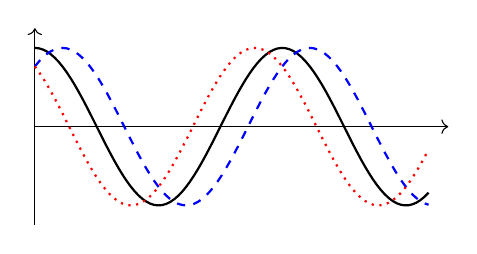
\begin{tikzpicture}[scale=0.5]
        % axis
        \draw[->] (0,0) -- (10.5, 0);
        \draw[->] (0,-2.5) -- (0, 2.5);
        % functions
        \draw[domain=0:10,black,thick,samples=100] plot (\x,{2*cos(deg(\x))});
        \draw[domain=0:10,blue,thick,samples=100,dashed] plot (\x,{2*cos(deg(\x-0.7))});
        \draw[domain=0:10,red,thick,samples=100,dotted] plot (\x,{2*cos(deg(\x+0.7))});
    \end{tikzpicture}
    \caption{实空间内波动方程的运动方向,虚线表示右移,点线表示左移}
\end{figure}
\chat{
我们从一维单色光的平面波出发,可以第一性地给出波函数 \eqref{eq:mono_wave_sol},其中 $C$ 是光强。实空间部分是完全离域的,它是一个球谐函数,可以从 $-\infty$ 到 $+\infty$ 的震荡,其中时间的部分表示传播的方向。这种离域性用来描述光的波动性没问题,但是无法描述粒子性。}
有无定域的波也满足波动方程?

\section{光波的波包}
动力学中常用\boldtext{波包}描述具有粒子行为的光波。定义
\begin{equation}
    \label{eq:wp_def} % wave packet definition
    \psi(x,t) = \int_{- \infty}^{+ \infty} A(k) \exp \big[ \ii \big( k x - \omega(k) t \big) \big] \, \mathrm{d} k,
\end{equation}
与单色光不同的是,其中放开了两个变量作为波数的函数——振幅 $A(k)$ 与频率 $\omega(k)$。
\chat{
对于单色光,给定了 $k$ 就确定了 $\omega$ 和波函数,所以一个 $k$ 就相当于一个单色光。对每一个的单色光的某种振幅分布的全空间积分,即为一种光的组合,称之为波包。为何称为「包」,后面从图像上解释。

于是 $A(k)$ 是光强振幅,描述波包的形状,$\omega(k)$ 是频率,描述波包的移动速度。
}

这个波包是否满足波动方程 \eqref{eq:mono_wave}?证明之。分别对坐标和时间求偏导,有
\begin{align*}
    \frac{\partial^2\psi(x,t)}{x^2} 
    &= \int_{-\infty}^{+\infty} A(k) \frac{\partial \ee^{\ii kx}}{\partial x^2} \exp(-\ii\,\omega(k) t) \,\dd k \\ 
    &= \int_{-\infty}^{+\infty} A(k) (-k^2) \frac{\partial \ee^{\ii kx}}{\partial x^2} \exp[\ii(kx - \omega(k)t)] \,\dd k,
\end{align*}
\begin{align*}
    \frac{\partial^2\psi(x,t)}{t^2} 
    &= \int_{-\infty}^{+\infty} A(k) \ee^{\ii kx} \frac{\partial}{\partial t^2}\exp(-\ii\,\omega(k) t) \,\dd k \\ 
    &= \int_{-\infty}^{+\infty} A(k) \left[-\omega(k)\right]^2 \ee^{\ii kx} \exp[\ii(kx - \omega(k)t)] \,\dd k, \\
\end{align*}
观察可知,当 $\omega(k) = ck$ 时,满足波动方程 \eqref{eq:mono_wave}。结论是,单色波的各种分布的组合同样满足波动方程。下面引入一种特殊的波包。

\suppInfo{波包与波动方程}{我们可以说,$\psi(x,t)$ 仍然是光波波动方程的解。这通过将上述 $\psi(x, t)$ 代入波动方程很容易验证。从物理的角度,事实上,如果表达式 $\omega(k) = c k$ 始终成立,那么被积函数 $\exp \big[ \ii \big( k x - \omega(k) t \big) \big]$ 就是波矢为 $k$ 的单色光。由于波动方程的特性,两个不同波矢 (或等价地说波长) 的单色光的线性叠加仍然是波动方程的解,而积分又可以看作是无数不同波长的光波的线性叠加,因此 $\psi(x,t)$ 仅仅就是复色光,它仍然满足单色光所满足的波动方程。

但是这种复色光有很有意思的特性,那就是我们可以通过合适地定义振幅 $A(k)$,使得 $\psi(x,t)$ 具有局域形状,并且该函数可以被归一化。我们应当注意到,单色光的表达式是不可归一化的,宏观上就是在全空间上宽度为常数的波形。}

\subsection{Gaussian 波包}

定义波包的振幅为 Gaussian 型函数,
\begin{equation}
    A(k) = \frac{\sqrt{a}}{(2 \pi)^{3/4}} \exp \left[ - \frac{a^2}{4} (k - k_0)^2 \right]. \label{eq:wp_gaussian_def}
\end{equation}

首先讨论,当 $t = 0$ 的时波包的情况,此时的波函数
\begin{equation}\label{eq:wp_t0}
\psi(x, 0) = \int_{-\infty}^{+\infty} \frac{\sqrt{a}}{(2 \pi)^{3/4}} \exp \left[ - \frac{a^2}{4} (k - k_0)^2 \right] \exp \left( i  k x  \right) \, \dd k. 
\end{equation}
为了求出这个积分,引入傅里叶变换(Fourier transform),
\begin{align}
    &F(x) = \int_{-\infty}^{+\infty} f(k) \ee^{\ii kx}\,\dd k, \\
    &f(k) = \frac1{2\pi}\int_{-\infty}^{+\infty} F(x) \ee^{\ii kx}\, \dd x, 
\end{align}
\chat{
其中 $f(x)$ 右侧的 $\frac{1}{2\pi}$ 也可拆成两个 $\frac1{\sqrt{2\pi}}$、将其中一个 $\frac1{\sqrt{2\pi}}$ 乘在 $F(x)$ 右边,这是傅里叶变换的多种等价表示方式。傅里叶变换可将时域 $f$ 变换为频域 $F$,相当于一种卷积,这里仅将它用作求积分公式。
}
Gaussian 函数的傅里叶变换为
\begin{align}
    &G(k) = \frac a{\sqrt \pi} \ee^{-a^2 k^2}, \\
    &g(x) = %\frac{1}{\sqrt{2\pi}} 
    \int_{-\infty}^{+\infty} G(k) \ee^{\ii kx} \dd k =  \frac{1}{\sqrt{2\pi}} \exp\left(-\frac{x^2}{4a^2}\right), \label{eq:ift_gaussian}
\end{align}
%{Gaussian 函数的逆变换}
\begin{lstlisting}
res = InverseFourierTransform[a/Sqrt[Pi] Exp[-a^2 k^2], k, x];
Simplify[res, Assumptions -> {a > 0}]
>> E^(-(x^2/(4 a^2)))/Sqrt[2 \[Pi]]
\end{lstlisting}
因此将 $t_0$ 时的波包,拼凑成傅里叶逆变换 \eqref{eq:ift_gaussian} 的形式,有
\begin{equation}
    \psi(x, 0) = \frac{\sqrt{a}}{(2 \pi)^{3/4}}  \ee^{i  k_0 x} \int_{-\infty}^{+\infty} \exp \left[ - \frac{a^2}{4} (k - k_0)^2 + i(k-k_0)x  \right] \dd k,
\end{equation}
设 $b = \frac a2$,$l = k-k_0$,则上式为
\begin{equation}
    \psi(x, 0) = \frac{2b}{(2 \pi)^{3/4}} \ee^{i  k_0 x} \int_{-\infty}^{+\infty} 
    \ee^{-b^2l^2} \ee^{\ii l x} \dd l, 
\end{equation}
凑出 \eqref{eq:ift_gaussian} 中的形式,在积分内乘 $\frac b{\sqrt{\pi}}$,同时令 $x = - 2\pi x'$,
\begin{align}
    \psi(x,0) &= \frac{2b}{(2 \pi)^{3/4}} \ee^{\ii k_0 x} \frac{\sqrt{\pi}}b \underbrace{\int_{-\infty}^{+\infty} \frac b{\sqrt{\pi}} \ee^{-b^2l^2} \ee^{\ii l (-2\pi x')} \dd l}_{\text{inverse Fourier transform}} \\
    &= \frac{2b}{(2 \pi)^{3/4}} \ee^{\ii k_0 x} \frac{\sqrt{\pi}}b  \exp\left(-\frac{\pi^2x'^2}{4 b^2}\right) \\
    &= \left(\frac{2}{a^2\pi}\right)^{1/4} \ee^{\ii k_0 x} \exp\left(-\frac{x^2}{a^2}\right). \label{eq:wp_photon_t0}
\end{align}
\begin{lstlisting}
Integrate[
 Sqrt[a]/(2 Pi)^(3/4)
   Exp[-a^2/4 (k - k0)^2] Exp[I k x], {k, -Infinity, Infinity}, 
 Assumptions -> {a > 0}]
>> (E^(x (I k0 - x/a^2)) (2/\[Pi])^(1/4))/Sqrt[a]
\end{lstlisting}
于是我们推导出了 0 时刻的 Gaussian 波包。%,并且该波包是归一化的,
%TODO: 并不归一吧

当 $t > 0$ 时,有
\begin{equation}
    \psi (x, t) = \left( \frac{2}{\pi a^2} \right)^{1/4} \exp \left[ - \frac{(x - ct)^2}{a^2} \right] \exp [ \ii k_0 (x - ct) ]. 
\end{equation}
\homework{
    \textbf{1.2}  利用傅里叶变换,推导 $t>0$ 的 Gaussian 波包。
}

\begin{figure}\centering
    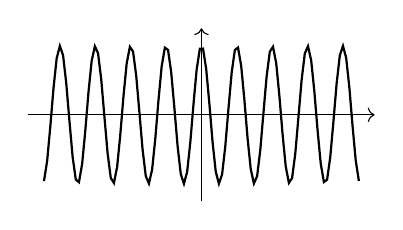
\begin{tikzpicture}[scale=0.5]
        % axis
        \draw[->] (-4.4,0) -- (4.4, 0);
        \draw[->] (0,-2.2) -- (0, 2.2);
        % functions
        \draw[domain=-4:4,black,thick,samples=100] plot (\x,{1.75*cos(deg(7*\x))});
    \end{tikzpicture}
    \begin{tikzpicture}[scale=0.5]
        % axis
        \draw[->,white] (0,-2.2) -- (0, 2.2);
        % functions
        \node[] at (0,0) {$\times$};
    \end{tikzpicture}
    \begin{tikzpicture}[scale=0.5]
        % axis
        \draw[->] (-4.4,0) -- (4.4, 0);
        \draw[->] (0,-2.2) -- (0, 2.2);
        % functions
        \draw[domain=-4:4,black,thick,samples=100] plot (\x,{1.75*exp(-0.25*\x*\x)});
    \end{tikzpicture}
    \begin{tikzpicture}[scale=0.5]
        % axis
        \draw[->,white] (0,-2.2) -- (0, 2.2);
        % functions
        \node[] at (0,0) {$=$};
    \end{tikzpicture}
    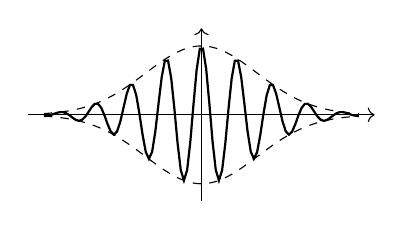
\begin{tikzpicture}[scale=0.5]
        % axis
        \draw[->] (-4.4,0) -- (4.4, 0);
        \draw[->] (0,-2.2) -- (0, 2.2);
        % functions
        \draw[domain=-4:4,black,thick,samples=100] plot (\x,{1.75*exp(-0.25*\x*\x)*cos(deg(7*\x))});
        \draw[domain=-4:4,black,samples=100,dashed] plot (\x,{1.75*exp(-0.25*\x*\x)});
        \draw[domain=-4:4,black,samples=100,dashed] plot (\x,{-1.75*exp(-0.25*\x*\x)});
    \end{tikzpicture}
    \caption{0 时刻波包的组成}
\end{figure}
\chat{
接下来探讨这个波函数有什么样的性质。一个全空间离域的单色波矢,乘上一个高斯函数,所以形成了这样一个波包。波与波包都是以光速 $c$ 向正方向传播,并且没有任何衰减、变形,最大振幅为 $\left( \frac{2}{\pi a^2} \right)^{1/4}$。
}

\section{实物粒子的 Gaussian 波包}
\chat{
德布罗意告诉我们,有静止质量的物体,既是波也是粒子。那么,实物粒子能不能用高斯波包来表示?单色光波的话有个很重要的关系 $\omega = kc$,频率和波矢有直接的关系,但是实物粒子不是这样的。现在我们要将光波波包向实物粒子过渡,以尝试从波动性的角度解释实物粒子。

但这里或许会遇到一个问题,实物粒子不会以 $c$ 的光速传播,因此 $\omega = ck$ 的表达式不成立。我们要如何定义角频率 $\omega$ 与波矢 $k$?
}

假设现在并不是狭义相对论的,或者说实物粒子以较低速度运动。在经典力学下,自由粒子 (不受外势场 $V (x)$ 影响的粒子) 的能量(即动量)为
\begin{equation}
    E = \frac{p^2}{2m}, \quad \text{for particle}
\end{equation}
考虑波粒二象性,粒子的能量必然也有物质波所对应的能量表述,
\begin{align}
    &E = h\nu = \hbar \omega, \\
    &p = \hbar k, 
\end{align}
上两式同样也适用于无质量的光子。对于实物粒子而言,联立上面的式子消去 $E,p$ 可得
\begin{equation}
    \omega = \frac{\hbar^2k^2}{2m},
\end{equation}
注意到,实物粒子的波矢与角频率是平方的关系,这是与光子最大的区别。

\chat{
同样使用波包 \eqref{eq:wp_def} 和高斯波包 \eqref{eq:wp_gaussian_def} 的原始定义,得到 $t =0$ 时刻的波函数与光波 \eqref{eq:wp_photon_t0} 是一样的,但 $t > 0$ 的波函数就完全不一样了。
}

\subsection{精确解}
尽管积分非常复杂,但这仍然是有解析解的。当 $t > 0$ 时,
\begin{equation}
    \psi(x,t) = \left(\frac{2}{\pi a^2}\right)^4 \frac1 {\sqrt{ 1 + \dfrac{2\hbar t}{ma^2}\ii}} \exp \frac {\displaystyle -\frac{x^2}{a^2}-\frac{\ii k_0^2 t \hbar }{2 m}+\ii
    k_0 x} {1 + \dfrac{2\hbar t}{ma^2}\ii},
\end{equation}
所以概率分布为
\begin{equation}
    |\psi(x, t)|^2 = \sqrt{\frac{2}{\pi a^2}} \frac{1}{\sqrt{1 + \displaystyle \frac{4 \hbar^2 t^2}{m^2 a^4}}} \exp \left[ - \frac{2}{a^2} \frac{\left( x - \displaystyle \frac{\hbar k_0}{m} t \right)^2}{1 + \displaystyle \frac{4 \hbar^2 t^2}{m^2 a^4}} \right]. 
\end{equation}

我们应当得到以下的结论:
\begin{itemize}[nosep]
  \item 指前因子可以表示波包的最大振幅。对于光波,其振幅恒定;但对于实物粒子,其振幅会依 $t$ 增长而递减,且递减的程度表现为类双曲线型;
  \item 指数项分母表示波包展宽。对于光波,其展宽恒定;但对于实物粒子,其展宽依 $t$ 增长而递增,且递增的程度表现为类双曲线型;
  \item 指数项分子表示波包的移动速度。对于光波,其移动速度为 $c$,与每个波矢 $k$ 分项的移动速度相同;而实物粒子的移动速度 (波包群速度) 为 $\hbar k_0 / m$,而波矢为 $k_0$ 的单色波对应的移动速度 (相速度) $\omega(k_0) = \hbar k_0 / 2m$,两者相差两倍。
\end{itemize}

这也就意味着,如果用 Gaussian 波包的方式描述自由粒子,即使规定 $t = 0$ 时具有较窄的波包展宽,足够长时间后也总会扩散。“足够长的时间”与物质的质量有关。假设电子的半径大约为 \SI{2.81E-15}{\metre};在一秒时间内仍然处于自由粒子状态。若使用波包解释,那么它现在的半径就在一秒钟内扩大了如下倍数:
\begin{equation}
\sqrt{1 + \frac{4 \hbar^2 t^2}{m_\mathrm{e}^2 r_\mathrm{e}^4}} 
= \sqrt{1 + \frac
{4\times(\num{1.05E-34})^2\times1}
{(\num{9.11E-31})^2(\num{2.82E-15})^4}
}
\simeq \num{2.92E25}
\end{equation}
\begin{lstlisting}
Clear[\[HBar], me, re]
\[HBar] = 1.05457182*10^-34;
me = 9.1093837*10^-31;
re = 2.8179*10^-15;
Sqrt[1 + (4 \[HBar]^2 1)/(me^2 re^4)]
>>2.91586*10^25
\end{lstlisting}
短短一秒,电子似乎会变得比太阳还要大。当然,对于宏观的物体而言,情况就不太一样了。假设一个人在宇宙大爆炸时期诞生,重 \SI{76}{\kilo\gram},想象成为 \SI{1}{\metre} 展宽的波,那么他可能在 2021 年时膨胀了 \num{7.20E-37} 倍。

\iffalse
目前为止,我们还不能说实物粒子波包的物理模型是错误的 (事实上,实物粒子波包模型确实是 Schr\"odinger 方程的解)。只有当物质质量足够大、初始时刻展宽足够宽时,波包能重现经典物理的图像。但想要通过波来刻画粒子的行为,似乎会在微观世界变得不太直观。我们会说这是朴素的波粒二象性的理解,它仍然是试图将粒子通过波的行为描述,而产生看似谬误的结论。

一种可能的理解是,所谓波性与粒性不应朴素地理解,物质的行为在长时间未观测时是不可知的;而在测量时,若使用检测波形的手段就会使得波函数坍缩到接近平面光波的形式;若使用检测粒子的手段则会使波函数接近 $\delta$ 函数的粒子形貌。这称为波包的收缩;依据一些量子力学表述,这比较接近关于波函数投影的假设。

但这不仅是 Gaussian 波包的困难。事实上,对于任意的 $A(k)$ 即任意波包,当时间足够长,波包总会弥散。这可以通过求取不确定度 $\langle x^2 \rangle - \langle x \rangle^2$ 给出;这需要使用到 Ehrenfest 定理。(Cohen-Tannoudji, LIII, Exercise 4)
\fi

\section{从自由粒子波函数到 Schr\"odinger 方程}

\subsection{非相对论 Schr\"odinger 方程}

Schr\"odinger 方程 \textbf{不可导出} ,它一般会作为量子力学的假定出现 (尽管说从 Dirac-von Neumann 公理体系能导出 Schr\"odinger 方程)。但若我们只考虑自由电子 (即不考虑外加势场),那么 Schr\"odinger 方程某种程度上可以通过波包函数导出。

我们仍然以实物粒子的波包函数出发:
\begin{gather}
  \psi(x, t) = \int_{- \infty}^{+ \infty} A(k) \exp \big[ i \big( k x - \omega(k) t \big) \big] \, \mathrm{d} k \\
  E = \hbar \omega \quad p = \hbar k \\
  E = \frac{p^2}{2 m} \quad \omega = \frac{\hbar k^2}{2 m}
\end{gather}
我们希望找到一个偏微分方程,使得 $\psi(x, t)$ 是该偏微分方程的解。但需要注意到,光波方程是不可行的,譬如 $\exp \big[ \ii \big( k x - \omega(k) t \big) \big]$ 满足下述方程
\begin{equation}
\frac{\partial^2 \psi}{\partial x^2} = \frac{k^2}{\omega^2} \frac{\partial^2 \psi}{\partial t^2} \quad \mathrm{(failed)}
\end{equation}
之所以这个方程在光波上允许,但粒子上不行,是因为对于光波,$k^2/\omega^2$ 恰好是 $1/c^2$ 为常数,但对于粒子而言则为 $(2m/\hbar k)^2$,并非是常数。上述描述波函数的方程只能用于 $k$ 是唯一值的情况,不能用于包含各种不同的 $k$ 的波包因此不应当使用该方程。

但很容易地会想到,之所以会出现 $\omega^2$ 是因为 $\psi$ 对时间 $t$ 作两次偏导时,其前面的系数 $\omega$ 也就被抽提了两次 (这对于 $k$ 也是类似的)。但如果现在只对 $t$ 作一次偏导,那么就只会抽提一次 $\omega$;并且 $k^2 / \omega$ 是常数 $2m/\hbar$,因此就解决了方程中出现的与 $k$ 有关的项。

沿着这个思路,我们就尝试对 $\psi(x, t)$ 分别作 $x$ 的二阶导、$t$ 的一阶导:
\begin{align}
  \frac{\partial^2 \psi}{\partial x^2} &= - \int_{- \infty}^{+ \infty} k^2 A(k) \exp \big[ i \big( k x - \omega(k) t \big) \big] \, \mathrm{d} k \\
  \frac{\partial \psi}{\partial t} &= - \int_{- \infty}^{+ \infty} \frac{i \hbar k^2}{2 m} A(k) \exp \big[ i \big( k x - \omega(k) t \big) \big] \, \mathrm{d} k
\end{align}
因此,
\begin{equation}
\frac{\partial \psi}{\partial t} = \frac{i \hbar}{2 m} \frac{\partial^2 \psi}{\partial x^2}
\end{equation}
即
\begin{equation}
i \hbar \frac{\partial \psi}{\partial t} = - \frac{\hbar^2}{2 m} \frac{\partial^2 \psi}{\partial x^2}
\end{equation}
这就是自由粒子所满足的 Schr\"odinger 方程。


\section{章节总结}
\courseTime{Sep. 19, 2022\\Week 3\\}

上周我们回顾了一下量子力学的诞生,这周课我们会讲算符、量子力学的公设。这这节课与物化AI的内容其实差不了太多,但是我们试图重新梳理,不是推导,演绎量子力学的发展历程,希望大家能加深理解。

如果大家做作业,包括对课程有任何的问题跟建议,都可以跟我们联系。

我们先来回顾上节课的内容,然后做一些基本的总结。因为每节课我也经常控制不好,有时想讲东西太多。事实上,有的关键点反而可能还会漏掉一些,所以我现在会来补一下。

上节课我们讲的,总结起来只有一页纸的内容,即量子力学的诞生。量子力学诞生,根本的地方其实就是在于对物质波粒二象性的理解,特别在微观世界中。波粒二象性最重要的关系就是 Planck--Einstein 关系式,
\begin{equation}
    E = h\nu = \hbar \omega
\end{equation}
这个公式,最早是由普朗克在拟合黑体辐射公式时,得到的一个新的物理概念。他发现,只有假设电磁波的辐射的话是一份一份进行的,才能拟合黑体辐射的频率(波长)跟辐射能之间的关系。

最重要的是说,光、电磁波,波的能量必须是一份一份的,所以每份能量跟波的频率直接成正比,并且这个相关的系数是一个常数,我们叫它 Planck 常量。后面经常会遇到 $\hbar$,$\hbar$对应的就是角频率角频率 $\omega$。
我们讲,一个粒子或者说一个东西,它是粒子。除了它的能量,那我们知道它的运动的话离不开动量。一个粒子,它的运动有方向、动量,并且动量也要满足动量守恒的规则。所以它必须有一个动量的表达式。动量的这个推导能证明,量子力学的诞生要基于相对论的诞生。没有相对论,我们没有办法直接给出光动量的方程式的。那么它到底是怎么来的呢?

在相对论的框架下面,有个质能关系。其中最重要的想法是,质量的变化满足
\begin{eqnarray}
    m = m_0 + \Delta m,
\end{eqnarray}
对于光而言的话,在相对论的框架下,
\begin{eqnarray}
    m = \frac{m_0}{\sqrt{1+\left(\frac vc\right)^2}}. 
\end{eqnarray}
所以当速度接近于光速的时候,$\Delta m \rightarrow \infty$。所以在相对论的框架下,光的初始质量一定是要为零,才能保证运动质量是常数。

对于任何物体或粒子,均有
\begin{equation}
    \left\{
        \begin{aligned}
            &\Delta E = \Delta m c^2,\\
            &p = mv,
        \end{aligned}
    \right.
\end{equation}
对于光子,
\begin{equation}
    \left\{
        \begin{aligned}
            &E = mc^2, \\
            &p = mc = \frac Ec = \frac{h\nu}c = \frac h\lambda, 
        \end{aligned}
    \right.
\end{equation}
可推知
\begin{equation}
    \left\{
        \begin{aligned}
            &E = h \nu = \hbar\omega , \\
            &p = \frac{h}{\lambda} = \hbar k, 
        \end{aligned}
    \right.
    \label{eq:photon_Ep}
\end{equation}
进而有
\begin{equation}
    \left\{
        \begin{aligned}
            &\omega = 2\pi\nu,
            &k = \frac{2\pi}{\lambda}, 
        \end{aligned}
    \right.
\end{equation}
于是 $\omega = ck$ 是线性关系。

到了实物波,我们通常处理的是在非相对论框架下的这个微观粒子——电子。目前不涉及重金属、过渡金属,特别是 F 区、镧系、锕系金属中的电子。我们通常处理氢元素中的电子,它的运动的速度是远低于光速的。
如何理解粒子的实物波?必须提到德布罗意的做法。他认为,实物也有波粒二象性,电子的干涉、衍射证明了波动的一面。波的性质是如何表述的呢?德布罗意认为,将普朗克-爱因斯坦的关系直接应用到实物波中。
以电子、质子为代表的微观粒子,静质量不为零 $m_0 \neq 0$,运动速度远低于光速导致 $\Delta m \simeq 0 |_{v \ll c}$,那么能量
\begin{eqnarray}
    E = \frac{p^2}{2m}.
\end{eqnarray}
这个公式是我们从牛顿力学就知道的。如果我们认为波动性跟粒子性是微观粒子的一体两面,那么它必定有波动的性质。那波动的性质所对应的物质波的角频率、物质波的波矢,跟粒子性是什么关系?德布罗意就把它们们两个强行耦合在一起。根据 \eqref{eq:photon_Ep},粒子的动量为
\begin{eqnarray}
    \hbar\omega = \frac{(\hbar k)^2}{2m},
\end{eqnarray}
因此得到 $\omega = \frac{\hbar k^2}{2m}$。
现在只是在演绎,怎么能够把非相对论框架下的薛定谔方程演绎出来。至于相对论框架的狄拉克方程,我们可以做其他方式的拓展。

为了更好地描述粒子实物波的粒子,上节课引入了 Gaussian 波包。我们先推导了自由粒子的波包,它的波动方程,
\begin{eqnarray}
    \psi(x,t) = A \exp[\ii (kx - \omega t)],
\end{eqnarray}
将不同波矢的自由粒子做一个全空间的积分或者组合,我们就可以得到一个波包,
\begin{eqnarray}
    \psi(x,t) = \int_{-\infty}^{\infty} A(k) \exp[\ii (k x - \omega(k) t)] \dd k,
\end{eqnarray}
最大的不同与,振幅 $A$、角频率都与波矢有关。

代入波动方程中,显然自由粒子的波包是满足的,
\begin{lstlisting}
\[Psi][x_, t_] := A Exp[I (k x - c k t)];
D[\[Psi][x, t], {x, 2}]/D[\[Psi][x, t], {t, 2}]
>> 1/c^2
\end{lstlisting}
但物质波的波包并不满足,
\begin{eqnarray}
    \frac{\partial^2 \psi}{\partial x^2} = \frac{4 m^2}{k^2 \hbar^2} \frac{\partial^2 \psi}{\partial t^2}. 
\end{eqnarray}
\begin{lstlisting}
\[Psi][x_, t_] := A[k] Exp[I (k x - (\[HBar] k^2)/(2 m) t)];
D[\[Psi][x, t], {x, 2}]/D[\[Psi][x, t], {t, 2}]
>> (4 m^2)/(k^2 \[HBar]^2)
\end{lstlisting}
左右两个偏导并不是线性关系。

上节课推导了物质波的波包。
注意到,如果物质波对坐标求二阶偏导、对时间求一阶偏导,二者是有线性关系的,即
\begin{eqnarray}
    \frac{\partial^2 \psi}{\partial x^2} = - \ii\frac{2m}\hbar \frac{\partial \psi}{\partial t}. 
\end{eqnarray}
稍作变化,便可发现
\begin{eqnarray}
    -\frac{\hbar^2}{2m} \frac{\partial^2 \psi}{\partial x^2} = \ii\hbar \frac{\partial\psi}{\partial t},
    \label{eq:free_partial_schrodinger}
\end{eqnarray}
这是自由粒子的薛定谔方程。这个没有严格推导,只有演绎。

\chapter{算符与量子力学公设}
对于定义,我会直接陈述。对于跟宏观世界不太一样的公设、算符,我们会展开讲。
微观世界中粒子的行为可以用什么波的状态方程来描述,如何得到体系中的可观测量物理量?
我们就需要算符作用到系统的波函数上,才能得到一些信息。首先,我们必须定义到底什么是算符,我们从一些常见的算符开始讲起。
\section{常见的算符}
对一个具体的波函数,它包含了该体系所有的信息。

那么对于任意一个算符 $\hat A$,相应的物理可观测量要怎么得到?假设算符 $\hat A$ 是时间的函数,定义有
\begin{eqnarray}
    \langle A(t) \rangle = \intinf \psi^*(x,t) \ \hat{A} \ \psi(x,t) \dd x,
\end{eqnarray}
对于位置算符,有
\begin{eqnarray}
    \langle x(t) \rangle = \intinf \psi^*(x,t) \ x\  \psi(x,t) \dd x,
\end{eqnarray}
位置算符就是位置本身,所以位置算符本身不是时间的函数。因为波函数本身包含时间,所以只对实空间积分就给出了波函数随时间演化的平均位置。也就说,在粒子散射的过程中,就可以通过这个方式给出粒子的平均运动轨迹。还是要强调,后面的推导并不是证明,只是演绎,希望能够增加理解。

\subsection{动量算符的推导}
大家知道动量算符是什么样子,它为什么是这个样子状态?跟宏观动量有何关系?为何与质量无关?

现在我们先回到牛顿力学中,有
\begin{eqnarray}
    p(t) = mv(t) = m \frac{\partial x}{\partial t},
\end{eqnarray}
无论在微观世界、宏观世界,还是在非相对论框架、相对论框架,这个是普适存在的。只不过说,在微观世界里面,如果体系的速度不是本征值的时候,那么我们要对速度求期望值,也就是速度的期望值也是动量的期望值。

在牛顿力学里,速度的描述是坐标,对时间的偏导是速度。如果我们在微观世界里,因为微观世界不确定这体系是不是坐标或动量的本征函数。那怎么办呢?我们就要对它们两个同时做期望值,两个期望一定满足
\begin{eqnarray}
    \langle p(t) \rangle = m \frac{\partial \langle x(t) \rangle}{\partial t},
\end{eqnarray}
这就是动量的公式在微观世界中的描述。

代入定义,有
\begin{eqnarray}
    \langle p(t) \rangle = m \intinf \frac{\partial}{\partial t} [\psi^*(x,t)\ x \ \psi(x,t)] \dd t,
\end{eqnarray}
利用复合函数求导的定义
\begin{eqnarray}
    \frac{\partial}{\partial x} [f(x) g(x)] = \frac{\partial f(x)}{\partial x} g(x) + f(x) \frac{\partial g(x)}{\partial x},
\end{eqnarray}
得到
\begin{eqnarray}
    \langle p(t) \rangle = m \intinf x \left(
        \frac{\partial \psi^*}{\partial t}\psi + \psi^* \frac{\partial \psi}{\partial t}
    \right)
    \dd t,
    \label{eq:pt_ave_2}
\end{eqnarray}
按照自由粒子的薛定谔方程 \eqref{eq:free_partial_schrodinger}, 上式 \eqref{eq:pt_ave_2} 有
\begin{align}
    & \frac{\partial \psi^*}{\partial t} = - \frac{\ii \hbar}{2m} \frac{\partial^2 \psi}{\partial x^2}, \\
    & \frac{\partial \psi}{\partial t} = \frac{\ii \hbar}{2m} \frac{\partial^2 \psi}{\partial x^2}, 
\end{align}
代回 \eqref{eq:pt_ave_2} 有
\begin{eqnarray}
    \langle p(t) \rangle = -\frac{\ii\hbar}{2} \intinf x \left( \psi \frac{\partial^2\psi^*}{\partial x^2} - \psi^* \frac{\partial^2\psi}{\partial x^2}\right) \dd x
    \label{eq:pt_ave_3}
\end{eqnarray}
约掉了质量 $m$。再次利用复合函数求导,设 $f(x) = \psi^*(x,t)$,$g(x) = \frac{\partial^2 \psi}{\partial x}$,则
\begin{align}
\frac{\partial}{\partial x}(f g) = \frac{\partial}{\partial x}\left(\psi^* \frac{\partial^2 \psi}{\partial x^2}\right) = \psi^* \frac{\partial^2\psi}{\partial x^2} + \frac{\partial \psi^*}{\partial x} \frac{\partial \psi}{\partial x}, 
\end{align}
于是有
\begin{align}
    &\psi^* \frac{\partial^2 \psi}{\partial x^2} = \frac{\partial}{\partial x} \left(\psi^*\frac{\partial \psi}{\partial x}\right) -\frac{\partial \psi^*}{\partial x} \frac{\partial \psi}{\partial x}, \\
    &\psi \frac{\partial^2 \psi^*}{\partial x^2} = \frac{\partial}{\partial x} \left(\psi\frac{\partial \psi^*}{\partial x}\right) - \frac{\partial \psi}{\partial x} \frac{\partial \psi^*}{\partial x},
\end{align}
代回 \eqref{eq:pt_ave_3} 有
\begin{eqnarray}
    \langle p(t) \rangle = \frac{\ii\hbar}2 \intinf x \frac{\partial}{\partial x} \left(\psi^* \frac{\partial \psi}{\partial x} - \psi \frac{\partial \psi^*}{\partial x}\right) \dd x,
    \label{eq:pt_ave_4}
\end{eqnarray}
设 $f(x) = \psi^* \frac{\partial \psi}{\partial x} - \psi \frac{\partial \psi^*}{\partial x}$,数学上显然有
\begin{eqnarray}
    \frac{\partial}{\partial x}[x f(x)] = f(x) + x \frac{\partial f(x)}{\partial x},
\end{eqnarray}
所以 \eqref{eq:pt_ave_4} 为
\begin{eqnarray}
    \langle p(t) \rangle = \frac{\ii\hbar}2 \intinf \frac{\partial}{\partial x}(x f(x)) \dd x - \frac{\ii\hbar}2 \intinf f(x) \dd x,
    \label{eq:pt_ave_5}
\end{eqnarray}
其中第一项为 $x f(x) |^{+\infty}_{-\infty}$。

\suppInfo{波函数的有限性}{
对于实际的原子分子体系,波函数必须在无穷远处趋于 0。比如坐标的平均值
\begin{eqnarray}
    \langle x(t) \rangle = \intinf \psi^*(x,t) \ x\  \psi(x,t) \dd x = \intinf x \rho(x,t) \dd x
\end{eqnarray}
是偶极,必然为有限值 $\psi^* x \psi |_{x \rightarrow \pm \infty} = 0$。同理,$\langle x^2 \rangle$为电四极,也必须为有限值。总之,波函数必须在无穷远处为 0。那么 $ \psi^*\psi|_{x=\pm\infty} \propto 1/x^s, s>2 $ ,应当比$ 1/x^n $更快衰减。}

于是 \eqref{eq:pt_ave_5} 为
\begin{eqnarray}
    \langle p(t) \rangle = - \frac{\ii\hbar}2 \intinf \left(\psi^* \frac{\partial \psi}{\partial x} - \psi \frac{\partial \psi^*}{\partial x}\right) \dd x,
\end{eqnarray}
再利用分部积分,有
\begin{align}
    \langle p(t) \rangle &= \frac{\ii\hbar}2 \intinf \left(\frac{\partial}{\partial x}(\psi\psi^*) - \frac{\partial \psi}{\partial x}\psi^* - \psi^* \frac{\partial \psi}{\partial x}\right) \dd x \\
    &= \psi\psi^* |_{-\infty}^{\infty} + \frac{\ii\hbar} 2 \intinf \left(-2\psi^* \frac{\partial \psi} {\partial x} \right)\dd x \\
    &= \intinf \psi^* \left(-\ii\hbar \frac{\partial}{\partial x}\right) \dd x,
\end{align}
那么 $\hat p = - \ii\hbar \frac{\partial}{\partial x}$。
通过动量的定义、薛定谔方程,便可演绎出动量算符。

动能算符
\begin{eqnarray}
    \hat T = \frac{\hat p^2}{2m} = -\frac{\hbar^2}{2m} \frac{\partial^2}{\partial x^2}
\end{eqnarray}
即薛定谔方程左边。

\section{含势函数的 Schr\"odinger 方程表达式}%与波函数空间-时间分离}
% credit: ZY Zhu

经过上述的演绎,可以知道非相对论自由粒子的薛定谔方程为
\begin{equation}
\ii \hbar \frac{\partial \psi}{\partial t} = \frac{\hat p^2}{2 m} \psi,
\end{equation}
其中的 $\hat p^2 / 2m$ 与经典力学中的动能项 $E = p^2 / 2m$ 非常相似。而经典力学中,哈密顿量可以写为动能项加势函数项。

类似地在上述方程中引入势函数 $V(x, t)$:
\begin{equation}
\ii \hbar \frac{\partial \psi}{\partial t} = \hat H \psi = \left( \frac{\hat p^2}{2 m} + V(x, t) \right) \psi
\end{equation}
上式就是含有势函数的、一般的 Schr\"odinger 方程,同时也定义了哈密顿算符 $\hat H$。它不只可以解释自由粒子,也可以解释受限粒子 (譬如一维势箱),但无法拓展到相对论的情形。化学中通常所使用的量子力学的最根源的表达式即上述 Schr\"odinger 方程。

特别地,讨论一种常见且特殊的情况,即势函数 $V(x, t) = V(x)$ 不随时间变化。势函数不随时间变化的例子,如自由的或外加静电场的分子电子运动过程,而势函数随时间变化的例子,如分子受光激发的过程。

当 $V(x, t) = V(x)$ 时,我们说该方程存在分离变量的 (空间-时间分离的) 波函数解。假定
\begin{equation}
\psi(x, t) = \phi(x) f(t),
\end{equation}
代入到 Schr\"odinger 方程,得到
\begin{equation}
\ii \hbar \phi(x) \frac{\partial f(t)}{\partial t} = - \frac{\hbar^2}{2 m} \frac{\partial^2 \phi(x)}{\partial x^2} f(t) + V \phi(x) f(t)
\end{equation}
两边分别除以 $\psi = \phi f$,得到
\begin{equation}
\frac{\ii \hbar}{f(t)} \frac{\partial f(t)}{\partial t} = - \frac{\hbar^2}{2 m} \phi(x) \frac{\partial^2 \phi(x)}{\partial x^2} + V 
%= \frac{\hat H \phi}{\phi}
\end{equation}
该式左右分别是只关于 $t$、$x$ 的函数。因此,若要让等式成立,则等式两边必为常数。该常数我们定作 $E$,因为哈密顿算符相当于表示体系的能量 (作为守恒量),
\begin{align}
    &\hat H \phi(x) = E \phi(x), \\
    &\pdv{t} f(t) = -\frac{\ii E}\hbar f(t),
\end{align}

那么,时间部分解得
\begin{equation}
f (t) = \exp \left( - \frac{i}{\hbar} E t \right),
\end{equation}
空间部分解得
\begin{equation}
\hat H \phi(x) \equiv \qty(- \frac{\hbar^2}{2 m} \pdv[2]{x} + V (x)) \phi(x) = E \phi(x)
\end{equation}
称为\boldtext{定态} Schr\"odinger 方程。

\extraInfo{推导}{
这两节课我一直在重复物化 A I 前几节课的内容,但是这里用一些比较数学演绎的方式,推导出方程的建立过程。

我希望大家能够体会其中的创造性,这个创造性是超越于一般的演绎和推理。现在经常讲机器学习、人工智能,人工智能为什么被认为说是有前途的一门学问呢?就是说它希望超越一般的规律,去寻找复杂大数据背后的一种数据到结果的映射关系。这个映射关系如果找到足够好,是不是可以从中得到一些物理?

对于物理、化学、生物,是研究物质的科学。为什么说化学叫中心学科呢?因为它下面是可以承接物理,往上可以承接更复杂的生物。「中心学科」只个是一个中性词,并不代表它最重要。整个过程三位一体,所有理论都是要以实验为基础开展科研工作。从实验中测得一种理论,同时要反过来解释甚至指导实验。

我们现在推导的薛定谔方程本身就是从实验中间抽取出来的,这是非常典型的范例。同时,后面也通过很多的推导去告诉大家,这里蕴含理论到底是有多强大,进而可以解释多少实验。这就是量子化学方向常常要做的事情,即解释化学中的现象。
}

不失一般性的将$ \hat p, \hat T, \hat V $从一维拓展到三维,则
\begin{align}
\hat p &= -\ii\hbar \left(\pdv{x}\vb{i} + \pdv{y}\vb{j} + \pdv{z}\vb{k}\right) = -\ii\hbar \bm\nabla, \\
\hat T &= -\frac{\hbar^2}{2m}\nabla^2, \\
\hat V &= V(x,y,z)
\end{align}
三维薛定谔方程 (3D SE)
\begin{equation}
\hat H \psi %= - \frac{\hbar^2}{2 m} \left( \frac{\partial^2 \phi}{\partial x^2} + \frac{\partial^2 \phi}{\partial y^2} + \frac{\partial^2 \phi}{\partial z^2} \right) + V (x, y, z) \phi 
\equiv - \frac{\hbar^2}{2 m} \nabla^2 \psi + V (x, y, z) \psi = E \psi,
\end{equation}
其中波函数可分离变量,写成\boldtext{定态} stationary 波函数与时间分量的乘积,
\begin{equation}
\psi(x,t) = \phi(x) \exp \qty( -\dfrac{i}{\hbar} Et).
\end{equation}
%这也是在物理化学 A I 课程中讨论得最多的方程,也是这门课程中最为重要的方程。
上述是单粒子的情形,如果是多粒子,可推广至
\begin{equation}
\qty( -\sum_i \dfrac{\hbar^2}{2m_i}\nabla_i^2 + V(x_1, \cdots, x_n)) \psi(x_1,\cdots,x_n) = E \psi(x_1,\cdots,x_n)
\end{equation}

% How. 这样我们已经可以把体系的确定了方程。
% 方程全部就给出来了对吧,因为它的这个试函数有可能是时间的关方程,所以它的哈密的方程有可能时间的方程。
% 特别的,如果我们的示函数与时间无关,那么我们就可以推出哈密顿的双层的话,也与时间无关,就等于动量上浮加上 VX 对吧。那么我们就可以翻成带带着。
% 好在这方向我们要再做一次,你们物化 AE 里面已经学过了,学过的这个变量分离变量了对吧,左边跟时间无关,右边跟时间有跟坐标无关对吧算幅我说的算幅,那么我就不失一般性的,可以把不函数写成什么,时间跟空间的层级吗?
% 对吧?那带入上时左边跟时间无关,我就可以把时间提前当成常量。
% 右边跟空间无关。
% 好了,现在我们做这个事情,下一步就要把左边的右边分开,左边右边分开,就是要让左边的 FT 消耗掉,右边的 yx 消耗掉。那这个两边同时重乘向重是除向整体的波函数。对吧。
% 这是 tree 那么就有,就可以导出这个的话就是。 Up np.
% 由此我们已经把坐标跟时间分开成两边,两边是无关的两个量,它们两个要相等,就意味着这两个要同时等于一个常数,否则的话他们是没法做这样的一个连力的。那么背后的意思就是我要把它分成两个方程了。
% 对吧,这两个方程好了,对于方程。
% 对方乘 2 我们知道说这样的一个形式,我们就可以 push 一般性的设置的 FT 为 A 乘上 ESP 的 at 对吧。那么把这个带进去就变成是其实这个也不用 A 到时候再说规划。就是 AFT 等于负I。
% A 等于负的 IE 除上H8,所以 FT 就等于。
% 那么方程1。
% 就是它的叫做定态确定和方式,因为它跟时间补完了对吧。
% 当然由此我们其实已经给出体系的再说一遍,我们现在其实这两节课我一直在重复,就是像固化 A1 里面很可能才第一节或者第二节的课对吧。但是这边我们用一些比较数学的一个演绎的方式,需要把那个早期这样的一个确定的方程的推导,这个过程的话展开来了解一下。
% 我希望大家能够体会细品中间的就是一种创造性,这个创造性的话是超越于一般的这种演绎跟推理。其实包括现在经常讲继续学习人工智能。人工智能为什么被认为说其实是挺有前途的一门学问呢?就是说他其实希望就是超越一般的规律,去寻找什么复杂的大数据背后的一个纷繁的数据背后的一种什么映射关系数据到结果的映射关系。那这个映射关系中如果找到足够好,是不是可以从中认得到一些物理?这个是蛮有意思的一个情况。因为我们对于我们物理化学是物理数学都是物理化学生物,我们称之为什么学科物质科学,物质科学可能是研究物质为主的一门科学。那我们为什么说化学叫中心学科呢?因为它是承接。
% 其实这个是一个中性词,并不代表它最重要,而正是因为说它是承接了什么物理的以及下面是可以承接物理,晚上是承接,晚上是可以承接更为复杂的生物对吧?那么整个过程那三三位一体其实背后对应就是所有东西都是要以所有都要以什么实验为基础开展的科研工作对吧?那么实验从实验中测一种理论的理论,同时要反过来的话解释甚至指导实验。那我们现在的确定和方程本身就是从从实验中间抽取出来的理论的一个非常典型的范例。然后同时我们后面也通过很多的证明,很多的那个推导去告诉大家这个这样的一个范例的话,推导得到的理论到底是有多强大,到底是可以真的解释多少实验?那么这就是后面我们做的量子化学里面常常要做的事情,就解释化学中的一些现象。那么有了定态学定要方程,我们这么还要再做一步对吧。因为真实的世界是什么?三维的世界首先它不是一维的。那么我们当然要不是一般性的干嘛把这些算图从一维的干嘛变成三维的,那这个是 strike forward 对吧。
% 那动量上浮。
% Full ih bar. 我们就要对它。 Exo. rising sandwich go to panda 那么我们就引入一个新的上浮的模式。
% 定态的,我们现在后面这节课,这次这门课我们根本都碰不到磐石的,当然下节课除外,所以我们这边就做这样的一个简单的定义。由此我们已经有了这个设定二方程的三维的普遍的普适的形式,动能算服加势能算服。
% 对。这边就是从这个应该就是单例子体系对吧,他的这个定态确定和方程当地词体系在真实世界中的定态确定和方程。那么由此我们其实已经可以把确定和方程的话。
% Particular culture in.
% 之所以称为定态训练方程,就是因为它的波函数并不包含时间。
% Stationery stay.
% 有了这些我们就可以开始讲这个前面我们就到这里为止,我们其实是把算幅的一些演绎给大家了。往下我们就要引入什么?为了完整性,一门课还是要完整性,可能大家已经学过了,那我们就是还要把算法的定义重新的抽题出来描述一下,以及它的一些基本的规则。
% 算幅的定义。算幅定义从本质上来讲的话,就是干嘛把一个函数干嘛变成了另外一个函数对吧,就它是把一个函数变另外还有一个操作。那么所以原则上说 A 可以是任何一个东西,可以是标量,可以是函数,可以是泛函。泛函的意思就是说它可以是根号偏微分之类的到动量动能上浮就是一个偏微分对吧?那么我们这边就有了到底它的代数规则。
% 上浮的和与差,就是说设。
% 那么这个算幅如果 C 等于 A 加 B 那么它做 C 作用在任何一个函数上,就是等于 A 作用的函数上加上 B 中文函数上,这个是不言而喻的对吧,也不需要说任何的。也就是说 C 无论是任何的一个函数算幅,它都满足这个。 Mm.
% 算符的乘法。设 C 等于 A 乘上 B 那么 C 就用在函数上,就等于把 A 跟 B 依次作用的函数先是 B 作用的函数上,然后 A 作用在 B 作用过之后的函数。
% 那么一般情况。
% 交换率是不成立的对吧?一般情况是这样,我们什么时候是这样的?如果这个函数比如说是一个坐标算幅跟势能算幅,它肯定是可以的对吧是吧?那么我们经常会讲的就是说如果我们的算幅一个是偏微分的算幅, B 的话就是一个坐标算幅。那么。
% 就在任何一个函数上,它是什么?它应该是这个 FX 加上 X 对吧?那它其实是等于什么呢? In jiangxi.
% 那另外一边的话,如果是 xa 先作用到这个函数上,那么它就是。
% 对吧?所以它们并不相等这个。当然我相信你们学过物化 A 一定知道这个乘法,它们交换率不成立。其实本身的话就对于说微观世界里面很多新颖的这种这样的现象对吧,比如说他的不完备性,他的这个他的测不准,甚至于什么后面的还有零点能这些东西都跟这相关,这后面慢慢会展开来讲。
% 等价上浮。若 A 作用到 F3 等于 B 作用的 F3 对于任意。
% 对任意函数都成立。
% 我们就说 A 等就是等于 B 好吧,那就像这边我们说的上面这个式子的话,这个是我们对于任一个函数做下来的对吧,FX我们没有定 FX 是什么东西好,所以这边就有就知道说这个。
% 就带 xm 等于什么这两个上头对吧,是等价的。
% 当我们在定义这个算幅空间的时候,为了完备性起见,我们肯定要定义它的什么单位算法称为单位算法,据说 1 就是它的单位算法。
% Unit operator tong shi ling weikong sanfu.
% Now operate. 同时我们这边做个约定,对于常数的算法。
% 我们都不加这个帽子。那么我们从前面也可以看到说这个。
% 就等于零,就是一个空胀符。好,那么上浮的最后的定义的话,行吧,那我们下节课再讲好。
% 作业的话,我会在下节课布置。
% 哪一个?就是那个减 1 等于就是那个半 X 那个减 1 等于0。
% 没就展示他们两个算不加价是完整,这只是为了完备性。其实后面可能到时候在后面会用到一些,但是本质上的话就是表示说这两个上浮是等价的,他们相应点基本是什么都没有,就是零售这是上浮空间。为了完备,你现在我们定义放射空间,我们只会定义说我们的那这块是要空间,我们定义的空间一定要给他完整全是数学项的一个,就是事实上我们用的不多。Ok。
% 然后之前那个就是那就是猜猜是分离的这是,时空分离什么地方不明白。
% 我说我也有问题。
% 行,大概就是就是从就是这里的话,把它变量分离之后。

到目前为止,我们已经演绎得到一些常见的算符。为了这门课的完整性,还要把算符的定义和基本规则重新抽提出来描述一下。


\section{算符的定义}
算符从本质上来讲,是把一个函数变成另外一个函数的操作。原则上说算符 $\hat A$ 可以是任何东西,可以是标量、函数、泛函等。如果算符是泛函,是说它可以是根号、偏微分之类的操作,比如动量算符就是偏微分。
\subsection{代数规则}

\begin{theorem}[算符的和与差]
    定义 $\CC = \AA + \BB$,那么
\begin{eqnarray}
    \CC u = \AA u + \BB u. 
\end{eqnarray}
\end{theorem}

\begin{theorem}[算符的乘法]
    设 $\CC = \AA \BB$,那么
\begin{eqnarray}
    \CC u = \AA\BB u = \AA (\BB u)
\end{eqnarray}
\end{theorem}

相信同学们学过物化一定知道这个乘法的交换律不成立,微观世界有很多新颖的现象,比如不完备性、测不准,甚至于后面会讲到的零点能等。

比如 $\AA = \frac{\partial}{\partial x}, \BB=x$, 有
\begin{align}
    \hat A \hat B f(x) &= \pdv{x} [x f(x)] = \qty(1 + \hat x \pdv{x}) f(x) \\
    \hat B \hat A f(x) &= x \pdv{x} f(x)
\end{align}

\begin{theorem}[等价算符]
    若 $\AA f=\BB f$ 对任意函数均成立,那么 $\AA =\BB$。
\end{theorem}
如
\begin{eqnarray}
    \frac{\partial}{\partial x} = 1 + \frac{\partial}{\partial x}.
\end{eqnarray}

\begin{theorem}[基本算符]
    单位算符 unit operator $\hat 1 = 1$,空算符 null operator $\hat 0 = 0$,常数算符通常不加 $\hat\cdot$。
\end{theorem}

% 
% 上午回顾了量子力学的诞生。
% 通过波粒二象性,隐入了实物波的波动方程,演绎出来薛定谔方程。
% 由此确立了微观粒子的状态也可以用波动方程描述。
% 对于波函数,状态与可观测量的关系,需要将算符作用上去,这是物化一的课程。
% 早上第二个内容就是演绎了动量算符为什么是偏微分的形式,并由一维拓展到高维,给出了定态薛定谔方程。
% 后面量化的大部分时间都会围绕定态薛定谔方程的求解,从定态薛定谔放成功可以得到物理化学光谱的信息。

% 第二部分,看一下算符的数学规则。
% 上午看了和差的定义是显而易见的,算符作用在函数上等于另一个函数,所以算符是定域的。$A$ 作用上去和 $B$ 作用上去是独立的。但是乘法不一样,$\hat A\hat B$ 依次作用上去。

% 一个典型的例子是导数算符和位置算符,导数算符可类比于之前推导的动量算符。

在其它表象下,算符本身可以构成完备集,算符本身可以描述微观状态,因此算符有各种加减乘除、单位元的定义,自然而然还有逆算符的定义。

\begin{theorem}[逆算符]
    设 $\hat A\hat B f(x) = f(x)$,我们就说 $\hat A = \hat B^{-1}$ 或 $\hat B = \hat A^{-1}$。
\end{theorem}

因此引申出很重要的概念\boldtext{对易}。

\begin{theorem}[对易]
    \begin{equation}
        [\hat A, \hat B] \equiv \hat A \hat B -\hat B \hat A
    \end{equation}
    若 $\hat A \hat B = \hat B \hat A$ 则$[\hat A,\hat B] = 0$,则称算符 $\hat A, \hat B$ 互易,否则不互易。
\end{theorem}

简单的例子,$\hat A = \frac{\partial}{\partial x}, \hat B = 3$,则二者互易。若 $\hat A = \frac{\partial}{\partial x}, \hat B = \hat x$, 则 $[\frac{\partial}{\partial x},\hat x] = 1$。

\homework{
    \textbf{1.} 请简化下列定义的算符 $\hat B$
    \begin{equation}
        \hat A = \frac{\partial}{\partial x} x, 
        \hat B = \hat A^2
    \end{equation}
    计算对易子 
    \begin{equation}
        \left[x^3, \frac{\dd}{\dd x}\right], \left[\frac{\dd}{\dd x}, 5x^2 + 3x + 4\right]. 
    \end{equation}
}
交换不成立,于是有了互易子的规律。以上是对于最普适算符给出的定义。

\subsection{线性算符}

对于量子力学中的算符,引入约定\boldtext{线性算符},指分别作用在两个函数上,
\begin{equation}
    \hat A [f(x) + g(x)] = \hat A f(x) + \hat A g(x)
\end{equation}
这个与加和有什么不同?加和是对所有算符成立,但是上式仅对线性算符成立。线性算符是说,一个算符作用在两个函数上,相当于分别作用在两个函数上。

引入线性算符的重要性:\boldtext{量子力学中所有具有物理意义的算符都是线性算符}。有一个重要的性质
\begin{equation}
    \hat A [C f(x)] = C\hat A f(x)
\end{equation}
\begin{equation}
    \hat A[ \underbrace{f(x) + \cdots + f(x)}_{C} ] = C\hat A f(x)
\end{equation}
哪些不是?$\sqrt{\cdot}, (\cdot)^2, \sin, \cos$ 等,比如
\begin{equation}
    \sqrt{f(x) + g(x)} \neq \sqrt{f(x)} + \sqrt{g(x)}. 
\end{equation}

哥本哈根诠释,表示波函数的平方表示概率。波函数本身没有物理意义,算符作用上去才有物理意义。

如果 $\hat A$ 是本征态,那么必然有
\begin{eqnarray}
    \hat A f(x) = A f(x), \\
    \hat A C f(x) = AC f(x)
\end{eqnarray}
任何的缩放也都是本征态,如果是非线性算符则无法满足。对于波函数而言,最重要的概念是叠加,干涉、衍射,是线性加和的,如果波函数不是线性的,那么波函数就不满足后面要学的量子力学公设。

有了这样的线性算符,就可以给出算符的\boldtext{左右分配律},
\begin{eqnarray}
    (\hat B + \hat C) \hat A = \hat B \hat A + \hat C \hat A,
\end{eqnarray}
左右分配律对任何算符一定成立,但是右分配律仅对线性算符成立。
\begin{eqnarray}
    \hat A (\hat B + \hat C)  \neq \hat A \hat B + \hat A \hat C,
\end{eqnarray}
算符里量化中用得不多,如果以后做实验,实验中越来越向微观调控发展。当你去操控分子,你的操作就对应于算符,需要先设计算符,算符必须是微观可观测的。可以做一些先验的设计,否则实验是不可能成立的。
\homework{\textbf{2.} 证明算符的左右分配律}

\subsection{Hermitian 算符与量子力学公设}

\begin{theorem}[Hermite 算符]
    对于任意给定的(合理)波函数 $u$,若算符满足
\begin{eqnarray}
    \int u^* \hat A u \dd \tau = \int(\hat A u)^* u \dd t,
\end{eqnarray}
则 $\hat A$ 为Hermite 算符。
\end{theorem}

如动量 $\hat p = -\ii \hbar \frac{\partial}{\partial x}$、动能 $\hat T = \frac{\hat p^2}{2m}$、哈密顿算符 $\hat H$。
\homework{\textbf{3.} 证明上述三个算符为 Hermite 算符}

为什么我们要隐入 Hermite 算符的定义?
清晰的客观物理事实,所有的物理可观测量都对应 Hermite 算符,期望值一定是实数。对应着
\begin{align}
    &\left\langle A\right\rangle = \int \psi^* \hat A \psi \dd \tau, \\ 
    &\left\langle A\right\rangle^* = \int \psi (\hat A \psi)^* \dd \tau = \int (\hat A \psi)^* \psi \dd \tau,
\end{align}
若 $\hat A$ 非 Hermite 则
\begin{eqnarray}
    \left\langle A\right\rangle \neq \ev{A}^*
\end{eqnarray}
$\ev{A}$ 不是实数,进而 $\hat A$ 不对应物理可观测量。

我们讨论的大部分算符不只是 Hermite 的,也都是线性的。
\homework{\textbf{4.} 对于线性的 Hermite 算符 $\hat A$,我们有
\begin{eqnarray}
    \int u^* \hat A \nu \,\dd \tau = \int (\hat A u)^* \nu \,\dd \tau,
\end{eqnarray}
同时,对于线性的 Hermite 算符,$\hat A, \hat B$ 具有以下性质,
\begin{enumerate}
    \item $\hat A + \hat B$ 仍是 Hermite 算符
    \item $[\hat A, \hat B] = 0$,$\hat A\hat B$ 与 $\hat B \hat A$ 仍是 Hermite 算符
\end{enumerate}

\textbf{5.}
    若 $\hat A, \hat B, \hat C$ 为线性算符
    \begin{enumerate}
        \item 若 $\hat A, \hat B$ 同时为 Hermite 算符,则 $\hat A \hat B + \hat B \hat A$ 与 $\ii [\hat A \hat B - \hat B \hat A]$ 都是 Hermite 算符
        \item $[\hat A, \hat B \hat C] = \hat B [\hat A, \hat C] + [\hat A, \hat B]\hat C$
        \item $[\hat A \hat B, \hat C] = \AA[\BB,\CC] + [\AA,\CC]\BB$
        \item $[\AA,[\BB,\CC]] + [\BB,[\CC,\AA]] + [\CC, [\AA, \BB]] = 0$
    \end{enumerate}
}

Hermite 算符之后,还有个重要的约定。

\subsection{Dirac 记号}

它是用来描述期望值。如果算符作用在波函数上,
\begin{eqnarray}
    \int \phi_m^* \hat A \phi_n \dd\tau = \langle \phi_m | \hat A | \phi_m \rangle \equiv \langle m | \hat A | m \rangle \equiv A_{mn}
\end{eqnarray}
如果 $m = n$ 则表示期望值,如果不等于则表示跃迁矩阵元,
\begin{eqnarray}
    A_{mn} \equiv \langle m | \hat A | n \rangle
\end{eqnarray}
% $\langle \phi_m | \hat A | \phi_m \rangle$ Dirac 记号,$A_{mn}$ 矩阵元表述,$\langle m | n \rangle = \int \phi_m^* \phi_n \dd\tau$ 重叠积分。所以
左矢表示 $\langle m| = \phi_m^*$ 波函数的共轭,右矢表示 $\ket{m} = \phi_m$ 波函数。还有更多自由的写法,
$\hat A n$ 自身可以看成一个函数,
\begin{eqnarray}
    \langle m | \hat A | n \rangle = \langle m | \hat A n \rangle,
\end{eqnarray}

所以 Dirac 记号右矢 $|n\rangle$ 代表波函数 $\phi_n$(即 $\hat A \phi_n$),左矢 $\langle m |$ 代表波函数 $\phi_m$(即 $\hat A \phi_m$)的共轭。

% \begin{eqnarray}
%     \int u^* \hat A \nu \dd\tau = \int(\hat Au)^* \nu \dd\tau, \\
%     \langle u | \hat A | u \rangle = \langle \hat A u | u \rangle = [][][][]
% \end{eqnarray}

通过 Dirac 记号,可以写出 Hermite 算符的定义:
\begin{equation}
  \langle m | \hat A n \rangle = \langle \hat A m | n \rangle = \langle n | \hat A m \rangle^* = \langle m | \hat A^* n \rangle
\end{equation}
对于 Hermite 算符而言,$\hat A = \hat A^*$。

但需要留意的是,当 $\hat A = \partial_x$ 即导数算符时,$\hat A^* = - \partial_x$;因此算符的共轭并非简单地将虚数单位 $\ii$ 替换为 $-\ii$。

我们把量子力学里算符简单过一遍。假设物化一里都学过,为了课程完整性所以需要讲一遍。这里跟以前学的有何不同?如果没有问题,下节课会讨论量子力学公设。如果有时间,我们会讨论物理意义和一些具体例子。

实验归纳总结了许多公理体系,即量子力学公设。目前还没有遇到违反公设的情况。多种公设的表述方式,在数学证明中都是等价的。

\begin{theorem}[公设1]
    一个量子力学体系,均可用一个含时的波函数 $\psi(\vec r, t)$ 来描述,该函数应是单值、连续和有限的品优波函数。
\end{theorem}

\begin{theorem}[公设2]
对于一个量子体系,每一个可观测力学量都对应一个线性 Hermite 算符与量子力学公设
\end{theorem}

\begin{theorem}[公设3]
当对量子体系的某一力学量进行测量时,每次可测一数值 $\lambda$ 则 $\lambda$ 与该力学量对应的算符以及波函数 $\psi$ 之间存在如下关系
\begin{eqnarray}
    \hat F \psi =\lambda \psi
\end{eqnarray}
即 $\lambda$ 是 $\hat F$ 的本征值,而 $\psi$ 是 $\hat F$ 的本征函数。
\end{theorem}

以前有同学问:为什么实验中的基态在测完之后还是在基态?化学中的实验,为什么能提前知道物质处在基态,为什么没有不确定性?比如为什么物质的生成焓都是确定的?我觉得这个问题非常好。

\begin{theorem}[公设4]
对于任意一个线性 Hermite 算符,其本征方程
\begin{eqnarray}
    \hat F \psi_i = \lambda_i \psi_i
\end{eqnarray}
的本征函数 $\{\psi_i\}$ 均构成一个完备集,对于任意一个波函数,
\begin{eqnarray}
    \Psi = \sum_i c_i \psi_i
\end{eqnarray}
都可以可以展开
\end{theorem}

这是一个非常强的定理,有它物理意义。一个原子的哈密顿算符,我们在物化1中解出了各种轨道。按第四点来说,这个完备基是在全空间展开的,也就是任何体系都可以用氢原子的完备基展开。比如两个相距一定距离的氢原子,物理上来说用两个波函数叠加是最好的,但从第四点来说,用一个原子的波函数来展开也是完全可行的。实际上,因为波函数是无穷多的,必须用无穷多才能完全描述,因此可以这么描述,但不是最高效的。

\subsection{Hermite 算符}
给出 Hermite 算符的特殊性质。不推导,留一些给同学们证明。

\begin{theorem}[a]
    线性 Hermite 算符的本征函数 $\{\psi_i\}$ 一定是正交归一的,Dirac 记号表述为
\begin{align}
    &\langle i | i \rangle = 1, \\
    &\langle i | j \rangle = 0, \quad i \neq j
\end{align}
推知
\begin{eqnarray}
    \delta_{ij} = 
    \left\{
        \begin{matrix}
            1, i=j,\\
            0, i\neq j
        \end{matrix}
    \right.,
\end{eqnarray}
\end{theorem}

\begin{theorem}[b]
    若$\psi$ 是算符 $\hat F$ 的本征值 $f$ 的本征函数,
\begin{eqnarray}
    \hat F \psi = f \psi,
\end{eqnarray}
则对 $\psi$ 体系,$\hat F$ 的一次测量肯定($100\%$)测得 $f$ 值。
\end{theorem}

\begin{theorem}[c]
若 $\Psi$ 不是 $F$ 的本征函数,按照第四点完备基的定义,总是可以表述成
\begin{eqnarray}
    \Psi = \sum_i c_i \psi_i, \quad\langle \Psi | \Psi \rangle = 1
\end{eqnarray}
如果是归一的,利用正交归一的性质
\begin{align}
    \langle \Psi | \Psi \rangle &= \Big\langle \sum_i c_i \psi_i \Big| \sum_j c_j \psi_j \Big\rangle \\
    &= \sum_i \sum_j c_i^* c_j \langle \psi_i | \psi_j \rangle \\
    &= \sum_i \sum_j c_i^* c_j \delta_{ij} \\
    &= \sum_i |c_i|^2 = 1.
\end{align}
\end{theorem}
算符的期望值
\begin{eqnarray}
    \langle F\rangle = \langle \Psi | \hat F | \Psi \rangle = \sum_i |c_i|^2 f_i. 
\end{eqnarray}
如果波函数并不是算符 $\hat F$ 的本征函数,每进行一次测量,平均值即为上式,每次测得的值为 $f_i$,概率为 $c_i$。

薛定谔猫是处在生态和死态叠加中,如果猫的状态是生和死的叠加,它并不是一定生或死的。那么数学上来说,我对某状态做某测量得到某值的概率是多少。

我们知道,动量算符和位置算符互易,不能同时测量,换句话说,它们不能同时拥有相同的本征函数。如果对动量的本征函数做位置的测量,也就是把位置的算符作用到动量的本征函数上去。
假设所有东西都是离散的。设 $\{\phi_i\}$ 为 $\hat p$ 的本征函数,一定不是位置算符的本征函数。将坐标作用上去,平均值为 $\int \phi_i^* \hat x \phi_i \dd \tau$。位置算符 $\hat x$ 的本征函数 $\{f_m\}$,将动量的本征函数展开为 $\phi_i = \sum_m c_i f_i$,所以在某个动量的本征函数 $\phi_i$ 上找到位于 $x_m$ 电子的概率就是 $|c_m|^2$,
测量后就有 $|c_m|^2$ 概率坍缩到 $f_m$ 上去。这个时候再测量位置,那么这个体系将永远处在 $f_m$ 上了。
如果再去测量动量,重新展开成 $f_m = \sum_i c_i \phi_i$,动量是全空间覆盖的,那么就有 $|c_i|$ 的概率处在 $\phi_i$ 态上。

我们在讨论化学问题的时候,总是在说基态能量、生成热,因为我们是对能量算符进行测量,所以基态的能量是不会变的,除非是基态和激发态的耦合或者是散射过程。

\begin{theorem}[d]
    若两个线性 Hermite 算符有一个共同的本征函数完备集,则两个算符可以对易,
\begin{eqnarray}
    \hat F \psi_i = f_i \psi_i. \hat G \psi_i = g_i \psi_i,
\end{eqnarray}
则二者互易 $[\hat F, \hat G] = 0$ 或二者可以同时测量
\end{theorem}

\homework{\textbf{6.} 证明 (a) 与 (d)}

为什么单值、连续、有限很重要?去年讲太慢了,很多没讲到。
我们用哥本哈根的统计诠释,讲品优波函数的物理内涵。

其实波函数本身没有物理意义,波函数的平方是概率,有物理意义。
\begin{eqnarray}
    |\psi (x,t)|^2 = \psi^*(x,t) \psi(x,t)
\end{eqnarray}
为概率密度 probability density,在 $t$ 时刻 $x$ 位置到 $x + \dd x$ 为之内发现粒子的概率,
\begin{eqnarray}
    |\psi(x,t)|^2\dd x = \text{Pr}(\dd x; x; t)
\end{eqnarray}
在区间 $[a,b]$ 内发现例子的概率,
\begin{eqnarray}
    \int_a^b |psi(x,t)|^2 \dd x = \text{Pr} (a \leqslant x \leqslant b, t)
\end{eqnarray}
全空间的概率和
\begin{eqnarray}
    \int_{-\infty}^{\infty} |\psi(x,t)|^2 \dd x = 1
\end{eqnarray}
$\psi$ 是归一化的 normalized。

由这些定义出发,品优波函数有哪些约束?

a) $|\psi|^2$ 是概率密度,可知 $|\psi(x,t)|^2 \dd x$ 有限。那么这个约定,是否意味着波函数在任何一点都要有限呢?实际上并不是很重要,其背后的数学表述是波函数必须平方可积的 square-integrable,才能保证波函数可以归一。这里有例外吗?第一节课我们就碰到过,自由粒子是全空间发散,下节课会讨论到。

在量子力学中,并不排除会使用某些不能归一化的波函数。\footnote{曾谨言 \S 2.1.6; Levine \S 2.4, \S 3.8}一个重要的例外就是自由粒子。波函数有限的定义可能不是很严谨。

\suppInfo{波函数一定为有限值才能平方可积吗?}
{
    假设在三位空间中 $x_0 $ 处,波函数存在孤立奇点 $ |\Psi(x_0)|^2 \rightarrow \infty $。看似违反了「有限」的公设,实际上,
	只需要 $\int_{\tau_0} |\psi(x)|^2 \dd[3] x$ 为有限值,在物理上就可以接受,
	$ \tau_0 $为包围$ x_0 $附近的任意小体积。
	
	取$ x_0 = 0 $,在球坐标下展开,
	\begin{align}
	\int_{\tau_0} |\psi(x)|^2 \dd[3] x &= \int_0^\pi \int_0^{2\pi} \int_0^{r_0} |\Psi(r,\theta,\phi)|^2 r^2\dd r \sin\theta\dd\theta \dd\phi \\
	&\propto \int_0^{r_0} |\Psi(r)|^2 r^2 \dd r \\
	&\propto \frac{r^3}{3} |\Psi(r)|^2 \Big|_0^{r_0}
	\end{align}
	当$ r_0 \rightarrow 0 $时,$r_0^3 |\psi(r_0)|^2 \rightarrow 0$,设 $\psi(r_0)| \rightarrow \frac1{r_0^s}$,则 $r_0^3 \frac{1}{r_0^{2s}} \rightarrow 0$,解得 $s < \frac32$。

    对于其它维度,可解得 二维$ s < 1 $、 一维$ s < \frac{1}{2} $。
}

b) 当 $x\rightarrow\pm\infty, \psi(x,t)\rightarrow0$,积分是全空间的,并且最终是有限的,所以在无穷远处一定为0。如果在无穷远处不为 0,肯定积分发散的。所以这一条也是概率密度推导出来的。

c) 为了满足哥本哈根学派的统计解释,要求归一化,全空间模的积分为1
\begin{eqnarray}
    \int_{-\infty}^{\infty} |\psi(x,t)|^2 \dd x = 1,
\end{eqnarray}
但归一化并不像想象中自发成立的。

问题,如果波函数在 $t = 0$ 是归一化的 $\int_{-\infty}^{\infty} |\psi(x,0)|^2 \dd x = 1$,那么它时间演化中的每一刻 $t>0$ 是否都是归一化的?请证明
\begin{eqnarray}
    \frac{\partial}{\partial t} \int_{-\infty}^\infty |\psi(x,t)|^2 \dd x =0, \rightarrow \int_{-\infty}^\infty \frac{\partial}{\partial t} |\psi|^2 \dd x =0,
\end{eqnarray}

证明,
% \begin{eqnarray}
%     \frac{\partial}{\partial t}|\psi|^2 = \psi \frac{\partial}{\partial t} \psi^* + \psi^* \frac{\partial}{\partial t}\psi
% \end{eqnarray}
% 代入薛定谔方程,有
% \begin{align}
%     &\ii\hbar \frac{\partial}{\partial t} \Psi = -\frac{\hbar^2}{2m} \frac{\partial^2}{\partial x^2} \psi + V(x) \psi, \\
%     &\frac{\partial}{\partial t} \psi = \frac{\ii\hbar}{2m} \frac{\partial^2\psi}{\partial x^2} - \frac{\ii}{\hbar} V(x) \psi, \\
%     123
% \end{align}
% 将后两式子代回 [][][],则有 【】【很长的式子,】【】
Schr\"odinger方程具有保持波函数归一化的特性。\footnote{顾樵 \S 2.1.2}证明如下

    	随时间演化满足含时薛定谔方程
    	\begin{equation}
    	\ii\hbar \pdv{t} \Psi = -\frac{\hbar^2}{2m} \pdv[2]{x}\Psi + V\Psi
    	\end{equation}
由
    \begin{align}
    \pdv{t} \Psi &= \dfrac{\ii\hbar}{2m} \pdv[2]{x} \Psi - \dfrac{\ii}{\hbar} V(x) \Psi \\
    \pdv{t} \Psi^* &= -\dfrac{\ii\hbar}{2m} \pdv[2]{x} \Psi^* + \dfrac{\ii}{\hbar} V(x) \Psi^*
    \end{align}
得
    	\begin{align}
    	&\phantom{=}\pdv{t} |\Psi(x,t)|^2  \\
        &= \pdv{\Psi^*}{t}\Psi + \Psi^*\pdv{\Psi}{t}  \\
    	&= \Psi \qty(-\dfrac{\ii\hbar}{2m} \pdv[2]{x} \Psi + \dfrac{\ii}{\hbar} V(x) \Psi) + \Psi^* \qty(\dfrac{\ii\hbar}{2m} \pdv[2]{x} \Psi - \dfrac{\ii}{\hbar} V(x) \Psi) \\
    	&= \dfrac{\ii\hbar}{2m} \qty[\Psi^*\pdv[2]{\Psi}{x} - \Psi\pdv[2]{\Psi^*}{x}] \\
    	&= \dfrac{\ii\hbar}{2m} \pdv{x} \qty[\Psi^*\pdv{\Psi}{x} - \Psi\pdv{\Psi^*}{x}]
    	\end{align}
那么
    \begin{align}
    \pdv{t} \intinf |\Psi(x,t)|^2 \dd x &= \intinf \dfrac{\ii\hbar}{2m} \pdv{x} \qty[\Psi^*\pdv{\Psi}{x} - \Psi\pdv{\Psi^*}{x}] \dd x \\
    & = \dfrac{\ii\hbar}{2m} \qty[\Psi^*\pdv{\Psi}{x} - \Psi\pdv{\Psi^*}{x}] \Big|_{-\infty}^\infty \\
   &= 0 
    \end{align}
 所以$ \intinf |\Psi(x,t)|^2 \dd x  $不依赖于时间。证毕。

甚至可以讲到高斯定理。

下节课真正开始求解真正体系了,我们会做一些拓展,展开数学推导中的黑箱。




\section{复习}
\courseTime{Sep. 26, 2022\\Week 4}
%2022-09-26 07:59:45  Wenbin Fan @FDU 
\chat{%
早上好。人少了一点,我们都是选了这课的。

第一次课回顾了量子力学的诞生,我们想从量子力学初期实验现象演绎出薛定谔方程。其中最重要的现象是波粒二象性。光波的波动方程是两个二阶偏导呈线性,薛定谔方程是二阶偏导、一阶偏导有线性关系。}

如果势函数 $V$ 与时间无关,那么则可以分离时间和坐标,对于仅包含坐标的方程为定态薛定谔方程。% 如果是自由粒子

2021 年,\emph{Science} 发布了《125 个问题:发现与发现》,其中 ``What is quantum uncertainty and why is it important?'' 是其中一个问题。\footnote{\url{https://www.science.org/content/resource/125-questions-exploration-and-discovery}}目前的量子计算、量子测量是热门领域。
\extraInfo{什么是量子不确定性,为什么它很重要?}{
海森堡不确定性原理是量子力学的一个关键原则,它指出我们不能同时测量一个物体的速度和位置。天文学家和科学记者Ethan Siegel写道:``你越是精确地测量一个物体的位置,你对其动量的了解就越是内在不准确。这不仅仅是我们仪器的失败,这种不确定性是宇宙的根本。''不确定性在量子计算中起着重要作用,它依靠电子叠加来存储信息。但是量子叠加是很棘手的事情。当你试图测量它们时,或者甚至通过与环境的共同作用,如遇到随机的电磁辐射脉冲,它们会坍缩(用量子术语)。
}

\chat{%
我们讲过了高斯波包。通过高斯波包一阶、二阶偏导之间的关联,我们演绎出了薛定谔方程,并且演绎出了光波可以回到麦克斯韦的波动方程。对于质量不为零的粒子,利用德布罗意物质波、波矢与角频率是二次关系,推出了薛定谔方程。
}

上次课讲了量子力学的公设,算符的定义。

1. 微观体系都需要波函数描述

2. 可观测量对应于线性 Hermite 算符。坐标、势函数的算符就是本身。 能量与动量的关系,$E = mc, p = h/\lambda$,加上薛定谔方程可推导出$\hat p = -\ii \hbar \frac{\partial}{\partial x}$

3. $\AA f = \lambda f$ 本征方程

4. 线性 Hermite 算符的本征函数 $\{\left|\phi_i\right\rangle\}$ 构成完备集,相同坐标空间和时间空间的系统内的任何一个粒子状态都可以表示成线性算符本征值的线性展开 $\ket{\psi} = \sum_i c_i \ket{\phi_i}$,由此就有关于测量的一些讨论。

\chat{%
下周放掉一节课,我们尽量讲两节课的内容。很多结论会直接给大家。
}

\chapter{粒子的平动}

\section{一维自由粒子}

势函数为 0,定态薛定谔方程
\begin{eqnarray}
    -\frac{\hbar}{2m} \frac{\partial}{\partial x^2}\psi(x) = E \psi(x),
\end{eqnarray}
设波函数 $\psi(x) = \ee^{s x}$,得到
\begin{eqnarray}
    s = \pm \frac{\ii}{\hbar} \sqrt{2m |E|}
\end{eqnarray}
利用德布罗意关系 $E = p^2 / 2m, p = \hbar k$,推出
\begin{eqnarray}
    E = \frac{\hbar^2k^2}{2m},
\end{eqnarray}
则
\begin{eqnarray}
    s = \pm \frac{\ii}{\hbar}|p| = \pm \ii |k| = \ii k,
\end{eqnarray}
正负号表示方向,所以正向波矢自身为正,前面符号也为正,故脱掉了绝对值符号,那么波函数为
\begin{eqnarray}
    \psi(x) = \ee^{\ii kx},
\end{eqnarray}
与负方向的波函数构成通解为
\begin{eqnarray}
    \psi(x) = C_1 \ee^{\ii kx} + C_2 \ee^{-\ii kx}
\end{eqnarray}
表示向右和向左传播的波。利用欧拉公式 $\ee^{\ii\theta} = \cos\theta + \ii\sin\theta$,展开为
\begin{eqnarray}
    \psi(x) = (C_1 + C_2) \cos kx + \ii (C_1 - C_2) \sin kx.  
\end{eqnarray}
\begin{lstlisting}
Subscript[C, 1] Exp[I k x] + 
  Subscript[C, 2] Exp[-I k x] // ExpToTrig
>> Cos[k x] Subscript[C, 1] + I Sin[k x] Subscript[C, 1] + 
 Cos[k x] Subscript[C, 2] - I Sin[k x] Subscript[C, 2]
\end{lstlisting}

\subsection{流密度}
\chat{%
流密度是说密度跟概率随时间流动的速度,对应着速度的概念。
}

回忆第一节课,我们讲到量子力学公设时提到,
状态波函数必须是正交归一的,意味着演化过程中的归一性质是不变的,使得
\begin{eqnarray}
    \int_{-\infty}^\infty |\psi(x,t)|^2 \dd x = 1
\end{eqnarray}
$\psi$ 归一化是不会随时间演化而破坏的,需要满足
\begin{eqnarray}
    \frac{\partial}{\partial t} \int_{\infty}^\infty |\psi|^2 \dd x = 0
\end{eqnarray}
概率必然大于零,可以将偏导放进去,
\begin{eqnarray}
    \int_{\infty}^\infty \frac{\partial}{\partial t}  |\psi|^2 \dd x = 0
\end{eqnarray}
有
\begin{eqnarray}
    \frac{\partial}{\partial t} |\psi|^2 = \frac{\partial}{\partial t} \psi^* \psi = \frac{\partial \psi^*}{\partial t}\psi + \psi^* \frac{\partial \psi}{\partial t}
\end{eqnarray}
代入薛定谔方程
\begin{eqnarray}
    \ii\hbar \frac{\partial}{\partial t} \psi = \left[
        -\frac{\hbar^2}{2m} \frac{\partial^2}{\partial x^2} + V(x,t)
    \right]
    \psi(x,t)
\end{eqnarray}
得到
\begin{eqnarray}
    \frac{\partial}{\partial t} |\psi|^2 = \frac{\ii\hbar}{2m} \frac{\partial}{\partial x}
    \left[
        \psi^* \frac{\partial \psi}{\partial x} - \psi \frac{\partial \psi^*}{\partial x}
    \right]
\end{eqnarray}
这是个很重要的式子,在哥本哈根诠释中,$|\psi|^2 = \rho(x,t)$ 是密度,所以粒子密度随时间的演化可以表示为
\begin{eqnarray}
    \pdv{t} \rho(x,t) = \pdv{x} \left[
        \frac{\ii\hbar}{2m} \left(
            \psi^* \pdv{\psi}x - \psi\pdv{\psi^*}x
        \right)
    \right]
\end{eqnarray}
对时间的偏导等于对坐标的偏导。流体力学中连续性方程
\begin{eqnarray}
    \frac{\partial \rho}{\partial t} + \frac{\partial J}{\partial x} = 0, 
\end{eqnarray}
其中流密度为
\begin{eqnarray}
    J = -\frac{\ii\hbar}{2m} \left( \psi^* \frac{\partial \psi}{\partial x} - \psi \frac{\partial \psi^*}{\partial x}\right)
\end{eqnarray}
应用高斯定理,可得连续性方程的积分形式
\begin{eqnarray}
    \underbrace{\frac{\partial}{\partial t} \underbrace{\int_V \rho \dd^3x}_{\substack{\text{粒子在体积} \\ \text{$V$ 中的概率}}} }_{\substack{\text{粒子流入或流出}\\ \text{体积 $V$ 的速度}}} 
     + 
    \underbrace{\oint_S \underbrace{J}_{\substack{\text{粒子流入或流出}\\ \text{体积 $V$ 的通量}}} \dd a}_{\text{围绕体积 V 的面积分}} = 0,
\end{eqnarray}
如果能够满足这个偏微分方程的平衡连续方程,该方程给出 $J$ 的定义就对应于粒子流入或流出某区域的速度。当体积固定、面积变大,速度的通量就变小了。这里的 $J$ 便是流密度。

对 $J$ 简单演绎,
\begin{align}
    J &= -\frac{\ii\hbar}{2m} \left( \psi^* \frac{\partial \psi}{\partial x} - \psi \frac{\partial \psi^*}{\partial x}\right) \\
    &= \frac{1}{2m} \left[
        \psi^* \left(-\ii\hbar\frac{\partial}{\partial x}\right) \psi +
        \psi \left(-\ii\hbar\frac{\partial}{\partial x} \psi\right)^*
    \right] \\
    &= \frac1{2m} \left[\psi^* \hat p \psi + (\hat p\psi)^* \psi\right]
\end{align}
因此,描述粒子运动的流密度可以由动量算符构造出来。

代入自由粒子的状态方程,
\begin{eqnarray}
    \psi(x,t) = a \exp (\ii k x) \exp \left( - \frac{\ii\hbar^2k^2}{2m}t\right), \quad k\hbar = p = mv,
\end{eqnarray}
%2022-09-26 08:33:07  Wenbin Fan @FDU
有
\begin{eqnarray}
    J = -\frac{\ii\hbar}{2m} [|a|^2 \ii k + |a|^2 \ii k] = \frac{\hbar k} m |a|^2 = |a|^2 v
\end{eqnarray}
流密度与速度成正比,可将 $J$ 看成粒子的运动速度。

\chat{%
可观测量对应的都是 Hermite 线性算符。某算符 $\AA$ 的期望值为,作用到状态波函数上并全空间积分,当且仅当状态函数为算符的本征函数时,算符作用上去得到本征值和本征函数。那么 $J$ 也应该当作算符,但是为什么没有?因为恰好自由粒子时动量函数的本征函数,所以全空间积分是一样的。

但是我们遇到了归一化问题。
}

\subsection{归一化问题}
一维自由粒子波函数的模方
\begin{eqnarray}
    \int_{-\infty}^\infty \psi^*\psi \dd x = |a|^2 \int_{-\infty}^\infty \dd x
\end{eqnarray}
显然是不可归一化的。
\chat{%
按照量子力学公设第一条,品优波函数描述微观粒子性质,但这里不能归一。所以结论是,不存在处于定态(给定 $k$)的自由粒子。
这里有些简单粗暴了,我们算出来是这个微观状态,但因为不能归一所以就断言不存在这样的状态。

对光而言,它没有初始状态,可以描述成这个状态。对粒子而言,波是内禀属性,不意味着静止的时候可以离散到全空间。我们推过光波的波包,随时间演化永远不会发散的。粒子的波包随时间弥散,这是不对的。
}

但是,不处于定态的自由粒子并非不可描述。自由粒子的定态波函数是动能算符 $\hat T$ 的本征函数,
\begin{eqnarray}
    \left\{\psi(x,t) = a \exp (\ii k x) \exp \left( - \frac{\ii\hbar^2k^2}{2m}t\right)
    \right\},
\end{eqnarray}
因为 $\hat T$ 是 Hermite 算符,所以构成完备集。任何一个粒子,不处于定态,就可以展开成全空间求和
\begin{eqnarray}
    \psi_0 (x,t) = \sum_k c_k\psi_k(x,t) = \int_{-\infty}^\infty c_k\psi_k (x,t) \dd k = \int_{-\infty}^\infty A(k) \psi_k(x,t) \dd k, \label{eq:wave_expand_fullSet}
\end{eqnarray}
表示成波包的样子。

\chat{%
这里有很多个人看法,不见得完全正确。我能保证最终结论是对的,保证数学推导肯定不错,但中间阐述是见仁见智的问题。本来量子力学背后就有很多种不同的解释。

假设一个粒子,我们准备好了它的初态,再也不给它任何的束缚,那么该粒子的演化一定遵循薛定谔方程。
}
%2022-09-26 08:44:08  Wenbin Fan @FDU

% 休息
% 第二节课 % 2022-09-26 08:53:53  Wenbin Fan @FDU

准备初态,
在实空间的表示形式
\begin{eqnarray}
    \psi(x,0) = \frac{1}{\sqrt{2\pi}} \intinf A(k) \ee^{\ii kx} \dd x, 
\end{eqnarray}
利用反 Fourier 变换关系,得到微观粒子处在第 $k$ 个态的概率,也就是在 $k$ 空间(动量空间)的概率分布,
\begin{eqnarray}
    A(k) = \frac{1}{\sqrt{2\pi}} \intinf \psi(x,0) \ee^{\ii kx} \dd x,
\end{eqnarray}
结合量子力学公设第四条,任何波函数都可以由另外一组波函数线性展开。

%2022-09-26 08:58:34  Wenbin Fan @FDU
构造一个自由粒子的初态,
\begin{eqnarray}
    \psi(x,0) = 
    \begin{cases}
        \frac1{\sqrt{2a}},\quad &x\in[-a,a],\\
        0, \quad &\text{其它}
    \end{cases}
\end{eqnarray}
这是一个阶梯函数,积分得到
\begin{eqnarray}
    A(k) = \frac1{\sqrt{2a}} \frac{\sin ak}{k}
\end{eqnarray}
在 $k$ 空间却是一个全空间的正弦函数,这在通讯领域中的数模转换时常用。
有了 $A(k)$ 之后可以用来构造波函数,参考式子 \eqref{eq:wave_expand_fullSet}
\begin{eqnarray}
    \psi(x,t) = \frac1{\sqrt{2\pi}} \intinf A(k,t) \ee^{\ii k x} \dd k. 
\end{eqnarray}

讨论 (1) 如果 $a$ 很小,束缚在很窄的一个范围内,那么
\begin{eqnarray}
    A(k) = \frac{1}{\pi a} \frac{\sin ak}{k} \approx \frac{\sqrt{a}}{\sqrt\pi}
\end{eqnarray}
与 $k$ 无关,表示动量展宽很大、不确定,位置确定

(2) 如果 $a$ 很大,
\begin{eqnarray}
    A(k) = \sqrt{\frac{a}{\pi}} \frac{\sin ak}{ak}
\end{eqnarray}
当 $k\rightarrow 0$ 时,$A(k)$ 取极大值,即 $|A(k)|^2$ 取极大值。此时位置不确定,动量确定。

\homework{
    \textbf{3.1}  对于给出下述初态 $\psi(x,t=0)$,即初始时刻自由粒子($V(x) = 0$)波函数,求出 $\psi(x,t)$ 含时演化波函数,其中 $a>0, b\in\mathbb{R}, x\in\mathbb{R}$,

    (a) $A \ee^{-a|x|}$, (b) $A\ee^{-ax^2}$, (c) $A \ee^{-ax^2} \ee^{-\ii b x}$. 
}

% 2022-09-26 09:09:14  Wenbin Fan @FDU
\section{一维势箱中的粒子}
\begin{figure}[tp]\centering
    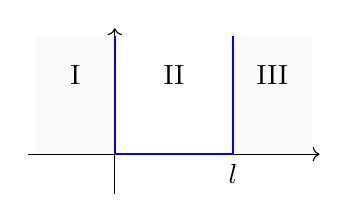
\begin{tikzpicture}[scale=0.5]
        % region
        \fill[lightgray] (-2,0) rectangle (0,3);
        \fill[lightgray] (3,0) rectangle (5,3);
        % axis
        \draw[->] (-2.2,0) -- (5.2, 0);
        \draw[->] (0,-1) -- (0, 3.2);
        % potential
        \draw[thick,blue] (0,0) -- (3,0);
        \draw[thick,blue] (0,0) -- (0,3);
        \draw[thick,blue] (3,0) -- (3,3); 
        % text
        \node[] at (-1,2) {I};
        \node[] at (1.5,2) {II};
        \node[] at (4,2) {III};
        
        \node[below] at (3,0) {$l$};
        % functions
        % \draw[domain=-4:4,black,thick,samples=100] plot (\x,{\x*\x});
    \end{tikzpicture}
    \caption{无限深势阱}
    \label{fig:inf_well}
\end{figure}
微观体系都是由品优波函数描述。
不管如何,先写出薛定谔方程。
\begin{eqnarray}
    \hat H \psi = (\hat T + V) \psi = E \psi,
\end{eqnarray}
势能函数
\begin{eqnarray}
    V(x) =
    \begin{cases}
        0, \quad &x\in [0,l]\\
        \infty, \quad &\text{其它}
    \end{cases}
\end{eqnarray}
薛定谔方程写为
\begin{align}
    (V-E) \psi &= \frac{\hbar^2}{2m} \pdv[2]{x} \psi \\
    \psi &= \frac{\hbar^2}{2m(V-E)} \pdv[2]{x} \psi,
\end{align}
对于 block I 和 III,$\psi(x) = 0$,对于 block II 有 
\begin{eqnarray}
    \psi(x) = C_1 \ee^{\ii k x} + C_2 \ee^{-\ii k x} = A \cos kx + B \sin kx,
\end{eqnarray}
这个解是普适的,导致体系量子化的是\boldtext{边界条件}。
%2022-09-26 09:15:15  Wenbin Fan @FDU
由边界条件来约束系统呈现出的状态,否则通解没有使用价值。

根据品优波函数的要求,波函数必须连续,
\begin{eqnarray}
    \psi(0) = \psi(l) = 0,
\end{eqnarray}
在 $x=0$ 处有
\begin{eqnarray}
    \psi(0) = A \cos 0 + B \sin 0 = 0,
\end{eqnarray}
立刻可得 $A = 0$,波函数为 $\psi(x) = B \sin kx$。在 $x=l$ 处,
\begin{eqnarray}
    \psi(l) = B \sin kl = 0,
\end{eqnarray}
得到量子化条件
\begin{eqnarray}
    k l = n \pi \rightarrow k = \frac{n\pi}{l}
\end{eqnarray}
其中 $n$ 为整数,所以该体系是量子化的。当 $n=0$ 时,舍去。由于 $n$ 为负时与 $n$ 为正时一样,没有新的物理,故令 $n \in \mathbb{N}^+$。得到解
\begin{eqnarray}
    \psi_n(x) = 
    \begin{cases}
        B \sin \frac{n\pi x}l, \quad &x \in [0,l], n\in\mathbb{N}^+, \\
        0,\quad &\text{其它}
    \end{cases}
\end{eqnarray}
% 【讨论为何只需要原函数连续,不需要高阶连续】【录音 1h 26min】
% 【n=0 为啥要舍去?补充】

\subsection{一维势箱的性质}

(1) 归一化 $\left\langle \psi_n \middle | \psi_n \right\rangle = 1$, 即
\begin{align}
    &= B^2 \int_0^l \sin^2 \frac{n\pi x}{l} \dd x \\
    &=  B^2 \int_0^l \left[\cos 0 - \cos \frac{2 n \pi x}l \right] \dd x \\
    &= \frac l2 B^2 + 0 = 1
\end{align}
其中利用了三角函数的变换
\begin{eqnarray}
    2\sin\alpha \sin\beta = \cos(\alpha-\beta) - \cos(\alpha+\beta),
\end{eqnarray}
因此,归一化条件为 $B = \pm \sqrt{\frac2l}$,波函数重写为
\begin{equation}
    \phi_n(x) = \begin{cases}\displaystyle
        \sqrt{\frac 2l} \sin\frac{n\pi x}l, \quad &x\in[0,l], n\in \mathbb{N}^+,\\
        0, \quad&\text{其它},
    \end{cases}
\end{equation}
注意到,归一化条件只与 $l$ 有关,与量子数 $n$ 无关。
\begin{lstlisting}
(* 画出一维势阱的波函数,n=0,...,5 *)
l = 1; (* 宽度 *)
Plot[Table[Sqrt[2/l] Sin[(n \[Pi] x)/l], {n, 0, 5}] // Evaluate, {x, 0, l}, Filling -> Axis]
\end{lstlisting}

(2) 不同量子数的波函数之间正交

当 $m \neq n$ 时,
\begin{align}
    \left\langle \psi_n \middle | \psi_n \right\rangle 
    &= \intinf \psi_n^* (x) \psi_m(x) \dd x \\
    &= \frac2l \int_0^l \sin \frac{n\pi x}{l} \sin \frac{n\pi m }{l} \dd x, \\
    &= \frac 1l \int_0^l \left[
        \cos \frac{(n-m)\pi x}l - \cos\frac{(n+m)\pi x}l
    \right] \dd x \\
    &= 0
\end{align}
因此波函数之间均满足正交归一,
\begin{eqnarray}
    \left\langle \psi_n \middle | \psi_n \right\rangle = \delta_{mn} = \begin{cases}
        1, \quad &m=n,\\
        0, \quad &m\neq n,
    \end{cases}
\end{eqnarray}

(3) 动量算符的平均值为 0
\begin{align}
    \ev{\hat p} 
    &= \left\langle \psi_n \middle| \hat p \middle| \psi_n \right\rangle \\
    &= - \ii \hbar \int_0^l \cos\frac{n \pi x}l \frac{\partial}{\partial x} \cos \frac{n\pi x}l \dd x \\
    &= \ii\hbar \frac{n\pi}l \int_0^l \cos \frac{n\pi x}l \sin\frac{n\pi x}l \dd x \\
    &= \frac{\ii\hbar}2 \frac{n\pi}l \int_0^l \left(\sin\frac{2n\pi x}{l} - \sin 0\right)\dd x \\
    &= \frac{\ii\hbar}2 \frac{n\pi}l \left(- \cos \frac{2n\pi x}l\right) \bigg|_0^l = 0,  
\end{align}
\begin{lstlisting}
Clear["Global`*"]
res = Integrate[
    Cos[(n \[Pi] x)/l] (-I \[HBar]) D[Cos[(n Pi x)/l], x], {x, 0, l}]
Simplify[res, Assumptions -> {n \[Element] Integers}]
>> 1/2 I \[HBar] Sin[n \[Pi]]^2
>> 0
\end{lstlisting}
其中利用了积化和差
\begin{equation}
    \sin\alpha \, \cos\beta = \frac12 \sin(\alpha+\beta) + \frac12 \sin(\alpha-\beta),
\end{equation}
所以流密度算符的平均值也为 0。

(4) 动量绝对值的平均值不为 0

首先求出动量平方的平均值,
\begin{align}
    \ev{\hat p^2} &= \langle \psi_n | \hat p^2 | \psi_m \rangle \\
    &= \frac{n^2\pi^2\hbar^2}{l^2} = \frac{n^2h^2}{l^2}
\end{align}
所以动量绝对值的平均值为
\begin{align}
    \rightarrow |p| = \sqrt{\ev{\hat p^2}} = \frac{n\hbar}{2l},
\end{align}
\begin{lstlisting}
res = 
Integrate[
    Sqrt[2/l] Cos[(n \[Pi] x)/l] (-I \[HBar])^2 D[
    Sqrt[2/l] Cos[(n Pi x)/l], {x, 2}], {x, 0, l}]
Simplify[res, 
    Assumptions -> {n \[Element] Integers}] /. {\[HBar] -> h/(2 Pi)}
>> (n \[Pi] \[HBar]^2 (2 n \[Pi] + Sin[2 n \[Pi]]))/(2 l^2)
>> (h^2 n^2)/(4 l^2)
\end{lstlisting}
即物质波长 $|p| = \frac{h}{\lambda}$, 得到 $\lambda = \frac h{|p|} = \frac{2l}n$。 

\extraInfo{不确定关系}{
    求出以下算符的平均值,
    \begin{align}
        &\ev{x} = \frac l2, \quad \ev{x^2} = \frac{1}{6} l^2 \left(\frac{3}{\pi^2 n^2}+2\right), \\
        &\ev{p} = 0, \quad \ev{p^2} = \left(\frac{n \pi\hbar}l\right)^2,
    \end{align}
    因此坐标和动量的涨落为
    \begin{align}
        &\sigma_p^2 = \ev{p^2} - \ev{p}^2 = \left(\frac{n \pi\hbar}l\right)^2, \\
        &\sigma_x^2 = \ev{x^2} - \ev{x}^2 = \frac{l^2}2 \left( \frac16 + \frac1{n^2\pi^2} \right),
    \end{align}
    所以不确定关系
    \begin{align}
        \Delta x \Delta p = \frac{\hbar}2 \sqrt{2+\frac{n^2\pi^2}3 } \ge \frac{\hbar}2
    \end{align}
    得到了验证。
}

(5) 能量的平均值

直接利用前面求解出的动量平方的平均值,有
\begin{align}
    E_n = \langle \hat T \rangle = \frac1{2m} \ev{\hat p^2} = 
    \frac{n^2h^2}{8ml^2}
\end{align}

(a) 由于 $n=0$ 不被允许,$E_1 = \frac{h^2}{8ml^2}$ 为\boldtext{零点能},

(b) 能级差
\begin{align}
    \Delta E_n = E_{n+1} - E_n = (2n+1) \frac{h^2}{8ml^2}
\end{align}
逐渐增大,表示能量不连续的情况越来越严重,这偏离了从量子到经典变化的过程。


(6) 粒子密度分布
\begin{eqnarray}
    \rho(x) = |\psi(x)|^2 = \frac 2l \sin^2 \frac{n\pi x}l, x\in[0,l]
\end{eqnarray}
波函数在区间 $(0,l)$ 中存在 $n-1$ 个节点,节点即 $\psi(x) = 0$ 的位置。观察易知,波函数的最大曲率与量子数 $n$ 有关,因此量子数越大,最大曲率也会越大。
\begin{lstlisting}
(* 粒子密度 *)
l = 1;
Plot[Table[2/l Sin[(n \[Pi] x)/l]^2, {n, 1, 5}] // Evaluate, {x, 0, 
  l}, Filling -> Axis]
\end{lstlisting}
当量子数趋于无穷,物质波波长越来越短,行为越像粒子,但是对于当前体系的波函数并不是这样。考察
\begin{eqnarray}
    \frac{\Delta E}{E} = \frac{2n+1}{n^2} \rightarrow 0
\end{eqnarray}
虽然能级差越来越大,但是能级差相对于总能量的比例是越来越小的。从另一个角度来说,当 $l$ 增大的时候,波函数会变得越来越扁长。

因此,从量子过渡到经典有两个判断标准。一是当量子数趋于无穷大时,波函数行为是否从离散变连续,是否有更多波的性质。二是当微观体系的尺寸变成宏观时,波函数的变化情况。

%2022-09-26 13:10:38  Wenbin Fan @FDU
% 下午课
%2022-09-26 13:26:28  Wenbin Fan @FDU
\homework{
    \textbf{3.2} (a) 一个 \SI{100}{\gram} 的实心球限制在 \SI{5}{\metre} 的线道上,(b) 束缚在 \SI{10E-10}{\metre} 区域内的电子。求以上两种情况的零点能。

    \textbf{3.3} 讨论如下定义的势箱中的粒子,
    \begin{equation}
        V(x) = 
\begin{cases}
    0, \quad &x\in \left[-\frac l2, \frac l2\right],\\
    +\infty, \quad &\text{其它},
\end{cases}
    \end{equation}
}

合并两次课的内容。都是一维薛定谔方程,势能都是 0 或无穷大。无限深势阱是束缚态。

% \subsection{一维势箱的应用}

%3.
\section{单侧有限深势阱}
\begin{figure}[tp]\centering
    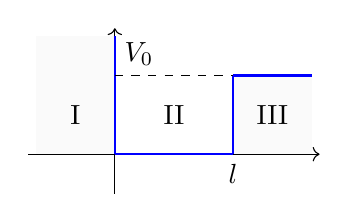
\begin{tikzpicture}[scale=0.5]
        % region
        \fill[lightgray] (-2,0) rectangle (0,3);
        \fill[lightgray] (3,0) rectangle (5,2);
        % axis
        \draw[->] (-2.2,0) -- (5.2, 0);
        \draw[->] (0,-1) -- (0, 3.2);
        % potential
        \draw[thick,blue] (0,0) -- (3,0);
        \draw[thick,blue] (0,0) -- (0,3);
        \draw[thick,blue] (3,0) -- (3,2); 
        \draw[thick,blue] (3,2) -- (5,2); 
        \draw[dashed] (0,2) -- (3,2);
        % text
        \node[] at (-1,1) {I};
        \node[] at (1.5,1) {II};
        \node[] at (4,1) {III};
    
        \node[below] at (3,0) {$l$};
        \node[above right ] at (0,2) {$V_0$};
        % functions
        % \draw[domain=-4:4,black,thick,samples=100] plot (\x,{\x*\x});
    \end{tikzpicture}
    \caption{半无限深势阱}
    \label{fig:half_inf_well}
    \end{figure}
先写出薛定谔方程
\begin{equation}
    \hat H = \hat T + \hat V(x),
\end{equation}
势能依然是分段函数,
\begin{equation}
    V(x) = 
    \begin{cases}
        +\infty, \quad &x\in(-\infty, 0),\\
        0, \quad &x\in[0,l],\\
        V_0, \quad &x\in(l,\infty),
    \end{cases}
\end{equation}

对于 block I,有
\begin{align}
    (V - E)\psi(x) &= \frac{\hbar^2}{2m} \frac{\partial \psi^2(x)}{\partial x^2} \\
    \psi(x) &= \frac{\hbar^2}{2m(V - E)} \frac{\partial^2 \psi(x)}{\partial x^2} = 0
\end{align}

对于 block II, 有
\begin{align}
    -\frac{\hbar^2}{2m} \pdv[2]{x} \psi(x) = E\psi(x),
    \label{eq:half_inf_block2_seq}
\end{align}
其通解为
\begin{equation}
    \psi(x) = C_1 \ee^{\ii k_{2}x} + C_2 \ee^{-\ii k_2 x}
\end{equation}
对应两个方向不同的波,由此引入了三个参数 $\{C_1, C_2, k_2\}$。将通解代入薛定谔方程 \eqref{eq:half_inf_block2_seq},解得 $k_2$ 与能量有关,
\begin{equation}
    E = \frac{\hbar^2}{2m} k_2^2 \rightarrow k_2 = \frac{\sqrt{2mE}}{\hbar},
\end{equation}

还是利用边界条件,求出待定参数。所有边条件都是跟品优波函数性质相关。

\textbf{边界条件 1},
\begin{equation}
    \psi(0^-) = \psi(0^+) = 0,
\end{equation}
容易得到
\begin{equation}
    C_1 \ee^0 + C_2 \ee^0 = 0,
\end{equation}
即
\begin{equation}
    C_2 = - C_1,
\end{equation}
由此将待定参数消掉一个。

对于 block III,
\begin{align}
    - \frac{\hbar^2}{2m} \pdv[2]{\psi(x)}{x} + V_0 \psi(x) &= E\psi(x), \\
    (V_0 - E) \psi(x)&= \frac{\hbar^2}{2m} \pdv[2]{x} \psi{x}
\end{align}
设 $\psi(x) = \ee^{sx}$,代回有
\begin{align}
    (V_0-E) \psi(x) &= \frac{s^2\hbar^2}{2m} \psi(x)
\end{align}
得到
\begin{eqnarray}
    s^2 = \frac{2m(V_0 - E)}{\hbar^2},
\end{eqnarray}
其中 $V_0 - E$ 的正负对结果有着决定性的影响。

当 $V_0 > E$ 时,称为\boldtext{束缚态},有
\begin{eqnarray}
    s = \pm k_3, \quad k_3 = \frac{\sqrt{2m(V_0 - E)}}{\hbar}, 
\end{eqnarray}
解得
\begin{eqnarray}
    \psi(x) = C_3 \ee^{k_3 x} + C_4 \ee^{-k_3 x},
    \label{eq:half_inf_block3_wf1}
\end{eqnarray}
%2022-09-26 13:47:16  Wenbin Fan @FDU
这时的未知参数有 $\{E, C_1, C_3, C_4\}$,其中 $E$ 是横跨三个 block 的变量,决定了 $k_2$ 和 $k_3$。接下来是一样的步骤,只要是可以精确求解的体系,比如稍复杂的氢原子,即不断引入边界条件,获得量子化的结果。

在 block I 负无穷($x=-\infty$),波函数一定为 0。在 block III 正无穷的区域,波函数一定会衰减为有限值,甚至是趋于 0 的,所以假定它不为无穷大。

\textbf{边界条件 2},
\begin{eqnarray}
    \psi(+\infty) = 0 
\end{eqnarray}
代入 \eqref{eq:half_inf_block3_wf1} 消掉了 $C_3$,还有三个待定参数 $\{E, C_1, C_4\}$。

\textbf{边界条件 3},在波函数 $x = l$ 的地方,左右波函数相等,
% 【引用 block II \& III 的波函数】
\begin{eqnarray}
    \psi(l^-) = \psi(l^+),
\end{eqnarray}
得到
\begin{eqnarray}
    C_1 \ee^{\ii k_2 l} - C_1 \ee^{-\ii k_2 l} = C_4 \ee^{-k_3 l}, \label{eq:half_condition_3}
\end{eqnarray}
还有两个待定参数。

边界条件 4,在 $x=l$ 的地方,左右波函数对坐标的偏导相等,
\begin{eqnarray}
    C_1 \ii k_2 \left[
        \ee^{\ii k_2 l} + \ee^{-\ii k_2 l} 
    \right] = - C_4 k_3 \ee^{-k_3 l} \label{eq:half_condition_4}
\end{eqnarray}
目前只剩能量 $E$ 待求。

依然使用欧拉方程,将 \eqref{eq:half_condition_3} \eqref{eq:half_condition_4} 展开成
\begin{align}
    & 2\ii \,C_1 \sin k_2l = C_4 \ee^{-k_3 l}, \\
    & 2 k_2 \ii \, C_1 \cos k_2 l = - C_4 k_3 \ee^{-k_3 l}, 
\end{align}
% [讨论为什么这么化简]
%2022-09-26 13:58:01  Wenbin Fan @FDU
左右两边分别相除
\begin{eqnarray}
    \frac1{k_2} \tan k_2l = - \frac1{k_3}. 
    \label{eq:half_inf_k2k3_0}
\end{eqnarray}
直接得到了 $k_2$ 和 $k_3$ 的关系,这样比较简单。如果分别求出 $C_1, C_4$ 和 $k_2, k_3$ 的关系,也可以讨论。

考虑到
\begin{eqnarray}
    k_2 = \frac{\sqrt{2mE}}{\hbar}, \quad k_3 = \frac{\sqrt{2m(V_0- E)}}{\hbar}, \label{eq:half_inf_k2k3_def}
\end{eqnarray}
代回 \eqref{eq:half_inf_k2k3_0},则得到能量相关的式子
\begin{eqnarray}
    \frac{\hbar}{\sqrt{2mE}} \tan \left(
        \frac l{\hbar} \sqrt{2mE}
    \right)
    = - \frac{\hbar}{2m(V_0 - E)},
    \label{eq:half_inf_k2k3_transcendental}
\end{eqnarray}
这是关于 $E$ 的超越方程,有数值解。

化简 \eqref{eq:half_inf_k2k3_transcendental},以便讨论。设
\begin{eqnarray}
    z = \frac{l}{\hbar} \sqrt{2mE}, \quad z_0 = \frac {l}{\hbar} \sqrt{2m V_0},\label{eq:half_inf_zz0_def}
\end{eqnarray}
可得
\begin{align}
    z_0^2 - z^2 &= \frac{l^2}{\hbar^2} 2m (V_0 - E),\\
    \sqrt{z_0^2 - z^2} &= \frac{l}{\hbar} \sqrt{2m (V_0 - E)},
\end{align}
所以 \eqref{eq:half_inf_k2k3_transcendental} 为
\begin{eqnarray}
    \frac{l}{z} \tan z = -\frac{l}{\sqrt{z_0^2 - z^2}},
\end{eqnarray}
将 $z$ 翻上去,有
\begin{eqnarray}
    \frac{z}{l} \cot z = -\frac{\sqrt{z_0^2 - z^2}}{l},
\end{eqnarray}
简单化简可得
\begin{eqnarray}
    \cot z = - \sqrt{\left(\frac{z_0}{z}\right)^2 - 1}. 
\end{eqnarray}
\begin{lstlisting}
(* 交互操作,查看 z0 变化时解的个数 *)
Manipulate[
    Plot[{Cot[z], -Sqrt[(z0/z)^2 - 1]}, {z, 0, 10}, 
        PlotRange -> {-6, 1}], {z0, 0, 20}]
\end{lstlisting}
\begin{figure}[tp]\centering
    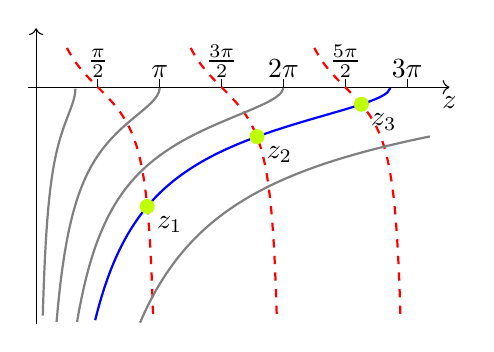
\begin{tikzpicture}[scale=0.5]
        % % region
        % \fill[lightgray] (-2,0) rectangle (0,3);
        % \fill[lightgray] (3,0) rectangle (5,2);
        % axis
        \draw[->] (-0.2,0) -- (10.5, 0);
        \draw[->] (0,-6) -- (0, 1.5);
        % text
        % \node[right] at (0,2) {I};
        \node[below] at (10.5,0) {$z$};
    
        \draw (pi/2,0) -- (pi/2,0.2);
        \node[above] at (pi/2,0) {$\frac{\pi}2$};
        \draw (pi,0) -- (pi,0.2);
        \node[above] at (pi,0) {$\pi$};
    
        \draw (3*pi/2,0) -- (3*pi/2,0.2);
        \node[above] at (3*pi/2,0) {$\frac{3\pi}2$};
        \draw (2*pi,0) -- (2*pi,0.2);
        \node[above] at (2*pi,0) {$2\pi$};
    
        \draw (5*pi/2,0) -- (5*pi/2,0.2);
        \node[above] at (5*pi/2,0) {$\frac{5\pi}2$};
        \draw (3*pi,0) -- (3*pi,0.2);
        \node[above] at (3*pi,0) {$3\pi$};
        % \node[above right ] at (0,2) {$V_0$};
        % functions
        \draw[domain=pi/4:pi-0.17,red,thick,dashed,samples=100] plot (\x,{cot(deg(\x))});
        \draw[domain=pi+pi/4:2*pi-0.17,red,thick,dashed,samples=100] plot (\x,{cot(deg(\x))});
        \draw[domain=2*pi+pi/4:3*pi-0.17,red,thick,dashed,samples=100] plot (\x,{cot(deg(\x))});
        
        \draw[domain=1.5:9,blue,thick,samples=100] plot (\x,{-sqrt(81/(\x*\x) - 1)});
        \draw[domain=0.17:1,gray,thick,samples=100] plot (\x,{-sqrt(1/(\x*\x) - 1)});
        \draw[domain=0.52:pi,gray,thick,samples=100] plot (\x,{-sqrt(pi*pi/(\x*\x) - 1)});
        \draw[domain=1.04:2*pi,gray,thick,samples=100] plot (\x,{-sqrt(4*pi*pi/(\x*\x) - 1)});
        \draw[domain=2.64:10,gray,thick,samples=100] plot (\x,{-sqrt(16*16/(\x*\x) - 1)});

        % roots
        \fill[draw, lime] (2.82259, -3.02769) circle[radius=5pt];
        \fill[draw, lime] (5.61016, -1.25442) circle[radius=5pt];
        \fill[draw, lime] (8.26182, -0.43206) circle[radius=5pt];
    
        \node[below right] at (2.82259, -3.02769) {$z_1$};
        \node[below right] at (5.61016, -1.25442) {$z_2$};
        \node[below right] at (8.26182, -0.43206) {$z_3$};
        
    \end{tikzpicture}
    \caption{半无限深势阱的解}
\end{figure}
当 $z_0 = 9$ 时,那么 $z$ 的取值是 $[0, z_0]$,画出图来看到只有 3 个解。对应于 3 个分离的束缚态 $E_i (i = 1, 2, 3)$,
\begin{eqnarray}
    E_i = \frac{\hbar^2 z^2}{2ml^2}, \quad i = 1, \cdots, N
\end{eqnarray}

最终给出半无限深势阱的波函数,
\begin{align}
    \psi_i (x) = 
    \begin{cases}
        0, \quad &x\in (-\infty, 0), \\
        C_1 \ee^{\ii k_2 x} - C_1 \ee^{-\ii k_2 x}, \quad &x\in[0,l],\\
        C_4 \ee^{-k_3 x}, \quad & x\in(l, \infty),
    \end{cases}
\end{align}
%2022-09-26 14:12:50  Wenbin Fan @FDU
% 将 $E_i$ 代入边界条件3中,得到
% \begin{align}
%     C_1 (\ee^{\ii k_2 l} - \ee^{-\ii k_2 l}) &= C_4 \ee^{-k_3 l}
% \end{align}
再给出\textbf{边界条件 5},波函数归一化
\begin{eqnarray}
    \intinf \psi^* \psi \, \dd x = 1,
\end{eqnarray}
由边界条件 3 \eqref{eq:half_condition_3} 和上式便可确定 $\{C_1, C_4\}$。边条件 3 中解得
\begin{equation}
    C_4 = C_1 \, 2\ii \,\ee^{k_3 l} \sin k_2 l,
\end{equation}
\begin{lstlisting}
Solve[Subscript[C, 1] (Exp[I k2 l] - Exp[-I k2 l]) == 
    Subscript[C, 4] Exp[-k3 l], Subscript[C, 4]] // 
  ExpToTrig // FullSimplify
>> {{Subscript[C, 4] -> 
   2 I E^(k3 l) Sin[k2 l] Subscript[C, 1]}}
\end{lstlisting}
由归一化条件可解得,
\begin{equation}
    C_1 = -\frac{\ii}2\left(
        \frac l2 + \frac1{2 k_3} \sin^2 k_2 l + \frac1{k_2} \sin 2k_2 l
    \right)^{-1/2}. 
\end{equation}
\begin{lstlisting}
res = Integrate[
    Subscript[C, 1] 2 I Sin[k2 x] Subscript[C, 1] 2 (- I) Sin[
        k2 x], {x, 0, l}] + 
    Integrate[
    2 I E^(k3 l) Sin[k2 l] Subscript[C, 1] Exp[-k3 x] 2 (-I) E^(k3 l)
        Sin[k2 l] Subscript[C, 1] Exp[-k3 x], {x, l, Infinity}, 
    Assumptions -> {k3 > 0}]
Solve[res == 1, Subscript[C, 1]] // FullSimplify
(* 运行结果略 *)
\end{lstlisting}

从以上 5 个边界条件,能给出量子化的条件。对于给定的 $z_0$ 能给出束缚态的解。

特别地,当 $z_0 < \pi/2$ 时,波函数将无解,不再有束缚态。不是只要有能垒就能束缚住电子。

% 2022-09-26 14:25:09  Wenbin Fan @FDU
% 第四节课
% 【画出波函数的图,拍照,黑、红、绿】

\boldtext{散射态}  $E > V_0$,解得
\begin{eqnarray}
    s^2 = \frac{(V_0 - E) 2 m}{\hbar^2} \rightarrow s = \pm \frac{\ii \sqrt{2m(E- V_0)}}{\hbar},
\end{eqnarray}
即
\begin{eqnarray}
    \psi(x) = C_3 \ee^{\ii k_3 x} + C_4 \ee^{-\ii k_3 x}, \quad k_3 = \frac{\ii\sqrt{2m(E-V_0)}}{\hbar},
\end{eqnarray}
这里有虚数,所以不能用无穷大的边界条件了。

\textbf{边界条件 3},
\begin{eqnarray}
    \psi(l^-) = \psi(l^+),
\end{eqnarray}
即
\begin{eqnarray}
    C_1 (\ee^{\ii k_2 l} - \ee^{-\ii k_2 l}) = 
    C_3 \ee^{\ii k_3 l} + C_4 \ee^{-\ii k_3 l}
\end{eqnarray}
\textbf{边界条件 4},
\begin{eqnarray}
    \psi'(l^-) = \psi'(l^+)
\end{eqnarray}
% 【检查上面的边界条件有没有 prime】
即
\begin{eqnarray}
    C_1 \ii k_2 (\ee^{\ii k_2 l} + \ee^{\ii k_2 l}) = \ii k_3 (C_3 \ee^{\ii k_3 l} - C_4 \ee^{-\ii k_3 l} )
\end{eqnarray}
省略推导过程,可以解出来
\begin{align}
    &C_3 = \frac12 \left[
        \left(1 + \frac{k_2}{k_3}\right) \ee^{\ii k_2 l} - 
        \left(1 - \frac{k_2}{k_3}\right) \ee^{-\ii k_2 l}
    \right] \ee^{-\ii k_3 l }C_1, \label{eq:half_inf_scat_c3}\\
    &C_4 = \frac12 \left[
        \left(1 - \frac{k_2}{k_3}\right) \ee^{\ii k_2 l} - 
        \left(1 + \frac{k_2}{k_3}\right) \ee^{-\ii k_2 l}
    \right] \ee^{\ii k_3 l} C_1, \label{eq:half_inf_scat_c4}
\end{align}
\begin{lstlisting}
Clear["Global`*"]
Solve[{Subscript[C, 1] (Exp[I k2 l] - Exp[-I k2 l]) == 
    Subscript[C, 3] Exp[I k3 l] + Subscript[C, 4] Exp[-I k3 l], 
    Subscript[C, 1] k2 (Exp[I k2 l] + Exp[-I k2 l]) == 
    k3 (Subscript[C, 3] Exp[I k3 l] - 
        Subscript[C, 4] Exp[-I k3 l])}, {Subscript[C, 3], 
    Subscript[C, 4]}] // FullSimplify
>> {{Subscript[C, 3] -> (
    E^(-I k3 l) (k2 Cos[k2 l] + I k3 Sin[k2 l]) Subscript[C, 1])/k3, 
    Subscript[C, 4] -> (
    E^(I k3 l) (-k2 Cos[k2 l] + I k3 Sin[k2 l]) Subscript[C, 1])/k3}}
\end{lstlisting}
%2022-09-26 14:34:13  Wenbin Fan @FDU

有几个结论,
(1) 注意到 $C_3^* = C_4$,可以知道 $\psi(x)$ 在 block III 是实三角函数,
(2) $k_2$ 与 $k_3(E)$ 没有任何限制要求,即本征值无限多,散射态是连续谱。因为没有其它可用的边界条件了,所以没有了量子化的能级。尽管这有点违背直觉。

\homework{
    \textbf{3.4}
    (1) 利用公式 \eqref{eq:half_inf_scat_c4},求
    $|C_1|^2$ 与 $|C_3|^2$ 
     的关系,并比较二者大小。
}

散射态的方程为
\begin{eqnarray}
    \phi (x) = \begin{cases}
        0, \quad &x \in (-\infty, 0), \\
        C_1 \ee^{\ii k_2 x} - C_1 \ee^{-\ii k_2 x}, \quad &x \in [0,l], \\
        C_3 \ee^{\ii k_3 x} + C_4 \ee^{-\ii k_3 x}, \quad &x \in (l, \infty),
    \end{cases}
\end{eqnarray}
直觉上来理解,$|C_1|^2$ 是粒子散射态反射回来的概率,$|C_3|^2$ 是投射过去的概率。

\homework{
    \textbf{3.4} (2) 推导并画出 $z = 12$, $z_0 = 9$ 时的体系波函数。
}

\section{阶梯势垒体系}
\begin{figure}[tp]\centering
    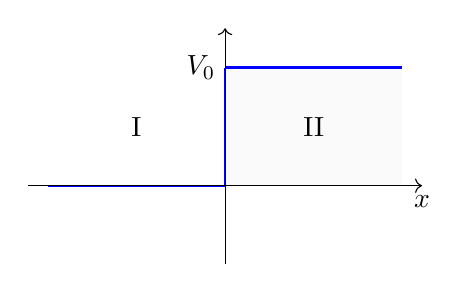
\begin{tikzpicture}[scale=0.5]
        % region
        % \fill[lightgray] (-5,0) rectangle (0,4);
        \fill[lightgray] (0,0) rectangle (4.5,3);
        \draw[blue,thick] (-4.5,0) -- (0,0);
        \draw[blue,thick] (0,0) -- (0,3);
        \draw[blue,thick] (0,3) -- (4.5,3);
        % axis
        \draw[->] (-5,0) -- (5, 0);
        \draw[->] (0,-2) -- (0, 4);
        % text
        \node[below] at (5,0) {$x$};
        \node[left] at (0,3) {$V_0$};
        \node at (-2.25, 1.5) {I};
        \node at (2.25, 1.5) {II};
    \end{tikzpicture}
\caption{阶梯势垒}
\end{figure}
\begin{eqnarray}
    V(x) = 
\begin{cases}
    0, \quad x\in(-\infty, 0), \\
    V_0, \quad x\in[0, \infty],
\end{cases}
\end{eqnarray}

对于 block I, 解出
\begin{eqnarray}
    \psi(x) = C_1 \ee^{\ii k_1 x} + C_2 \ee^{- \ii k_2 x},
\end{eqnarray}
其中
\begin{eqnarray}
    k_1 = \frac{\sqrt{2mE}}{\hbar}
\end{eqnarray}
有三个待定参数 $\{C_1, C_2, E\}$。

对于 block II,与单侧无限深势阱中的 block III 是一致的。
% 【直接复制过来上面的求解,已拍照】
%2022-09-26 14:46:05  Wenbin Fan @FDU

\boldtext{散射态} $E > V_0$,推出
\begin{eqnarray}
    S = \pm \ii k_2, \quad k_2 = \frac{\sqrt{2m(E-V_0)}}{\hbar}
\end{eqnarray}
波函数
\begin{align}
    \psi(x) = \begin{cases}
        C_1 \ee^{\ii k_1 x} + C_2 \ee^{\ii k_1 x},\quad & x \in (-\infty, 0), \\
        C_3 \ee^{\ii k_2 x} + C_4 \ee^{\ii k_2 x}, \quad & x \in [0, \infty),
    \end{cases}
\end{align}
有 5 个待定参数 $\{C_1, C_2, C_3, C_4, E\}$。

% 【画图】
多个动量本征态的叠加。
% $C_1$ $C_3$ 都是向右方向的动量本征矢。
\begin{figure}[tp]\centering
    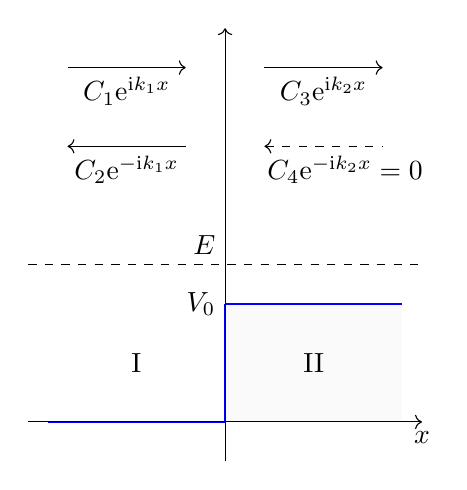
\begin{tikzpicture}[scale=0.5]
        % region
        % \fill[lightgray] (-5,0) rectangle (0,4);
        \fill[lightgray] (0,0) rectangle (4.5,3);
        \draw[blue,thick] (-4.5,0) -- (0,0);
        \draw[blue,thick] (0,0) -- (0,3);
        \draw[blue,thick] (0,3) -- (4.5,3);
        % axis
        \draw[->] (-5,0) -- (5, 0);
        \draw[->] (0,-1) -- (0, 10);
        % text
        \node[below] at (5,0) {$x$};
        \node[left] at (0,3) {$V_0$};
        \node at (-2.25, 1.5) {I};
        \node at (2.25, 1.5) {II};
        %
        \draw[dashed] (-5, 4) -- (5, 4);
        \node[above left] at (0,4) {$E$};
        %
        \draw[->] (-4,9) -- (-1,9);
        \node[below] at (-2.5, 9) {$C_1 \mathrm{e}^{\mathrm ik_1 x}$};
        \draw[<-] (-4,7) -- (-1,7);
        \node[below] at (-2.5, 7) {$C_2 \mathrm{e}^{-\mathrm ik_1 x}$};
        \draw[->] (1,9) -- (4,9);
        \node[below] at (2.5, 9) {$C_3 \mathrm{e}^{\mathrm ik_2 x}$};
        \draw[<-,dashed] (1,7) -- (4,7);
        \node[below] at (2.5, 7) {$\phantom{0=}C_4 \mathrm{e}^{-\mathrm ik_2 x} = 0$};
    
        % functions
        % \draw[domain=pi/4:pi-0.17,red,thick,dashed,samples=100] plot (\x,{cot(deg(\x))});
    \end{tikzpicture}
    \caption{波的方向示意图}
\end{figure}

概率流密度的定义
\begin{eqnarray}
    J = \frac{\ii\hbar}{2m} \left[
        \psi^* \pdv[x] \psi - \psi \pdv[x] \psi^*
    \right]
\end{eqnarray}
对于 block I,
\begin{eqnarray}
    J_1 = \frac{k_1 \hbar}{m} \left(
        |C_1|^2 - |C_2|^2
    \right)
\end{eqnarray}
这个体系中的截面只有一条线,流入为负,流出为正,因此
$\frac{k_1 \hbar}{m} |C_1|^2$ 为进入 block I 入射波($C_1 \ee^{-\ii k_1 x}$)的概率流密度,
同理 $\frac{k_1 \hbar}{m} |C_2|^2$ 为反射波($C_2 \ee^{-\ii k_2 x}$)的概率流密度,因此可得 $\frac{k_2 \hbar}{m} |C_3|^2$ 为进入 block III 的波($C_3 \ee^{\ii k_3 x}$)的概率流密度,特别地,$\frac{k_2 \hbar}{m} |C_4|^2 = 0$,因为不会有反射回来的波,所以 $C_4 = 0$。

思考,一个能量为 $E$($E>V_0$)的粒子从 $\infty$ 向 $-\infty$ 传播,此时边界条件 3
\begin{eqnarray}
    \psi(0^-) = \psi(0^+),
\end{eqnarray}
推出
\begin{eqnarray}
    C_1 + C_2 = C_3,
\end{eqnarray}
边界条件 4
\begin{eqnarray}
    \psi'(0^-) = \psi'(0^+)
\end{eqnarray}
推出
\begin{eqnarray}
    k_1 (C_1 - C_2) = k_2 C_3,
\end{eqnarray}
联立解得
% 【见照片,有 ref】
%2022-09-26 15:02:08  Wenbin Fan @FDU
% 【k1 k2 def】【没拍全】
\begin{align}
    & C_2 = \frac{k_1 - k_2} {k_1 + k_2} C_1, \\
    & C_3 = \frac{k_1}{k_1 + k_2} C_1,
\end{align}

定义反射系数
\begin{eqnarray}
    R = \frac{ \displaystyle \frac{k_1 h}m |C_2|^2 } { \displaystyle \frac{k_1 h}m |C_1|^2 } = \frac{(k_1 - k_2)^2} {(k_1 + k_2)^2}, 
\end{eqnarray}
定义透射系数,
\begin{eqnarray}
    T = \frac{ \displaystyle \frac{k_2 h}m |C_2|^2 } { \displaystyle \frac{k_1 h}m |C_1|^2 } = \frac{4k_1k_2} {(k_1 + k_2)^2}, 
\end{eqnarray}
显然有 $R^2 + T^2 = 1$。

代入 $k_1, k_2$ 的定义
\begin{eqnarray}
    R = \left( 1 - \sqrt{1 - \frac{V_0}E}\right)^2 
    \left( 1 + \sqrt{1 - \frac{V_0}E}\right)^{-2},
\end{eqnarray}
当 $0 < \frac{V_0}{E} < 1$ 时,
% 【画图 R - (V0/E) 的图,类似 $x^2$ 的图】
哪怕到了 $\frac{V_0}E = 80\%$,透射率只有 15\%,当 $E = V_0$ 时全反射,并不是像想象中的那样越过去。
\begin{lstlisting}
(* 画出 R-(V0/E) 的图 *)
Plot[(-1 + Sqrt[1 - x])^2/(1 + Sqrt[1 - x])^2, {x, 0, 1}, 
    PlotRange -> {0, 1}]
\end{lstlisting}

\section{有限高方势垒}
\begin{figure}[tp]\centering
    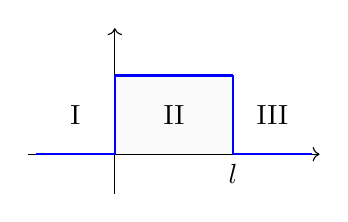
\begin{tikzpicture}[scale=0.5]
        % \fill[lightgray] (-2,0) rectangle (0,3);
        \fill[lightgray] (0,0) rectangle (3,2);
        % axis
        \draw[->] (-2.2,0) -- (5.2, 0);
        \draw[->] (0,-1) -- (0, 3.2);
        % potential
        \draw[thick,blue] (-2,0) -- (0,0);
        \draw[thick,blue] (0,0) -- (0,2);
        \draw[thick,blue] (0,2) -- (3,2);
        \draw[thick,blue] (3,0) -- (3,2); 
        \draw[thick,blue] (3,0) -- (5,0);
        % text
        \node[] at (-1,1) {I};
        \node[] at (1.5,1) {II};
        \node[] at (4,1) {III};
        
        \node[below] at (3,0) {$l$};
        % functions
        % \draw[domain=pi/4:pi-0.17,red,thick,dashed,samples=100] plot (\x,{cot(deg(\x))});
    \end{tikzpicture}
    \caption{有限高方势垒}
    \end{figure}
势能的形式,
\begin{eqnarray}
    V(x) = 
        \begin{cases}
            0, \quad &x \in (-\infty,0),\\
            V_0, \quad &x \in[0,l],\\
            0, \quad &x \in (l, \infty),
        \end{cases}
\end{eqnarray}

分情况讨论,$E<V_0$ 时,得到波函数
\begin{eqnarray}
    \psi(x) =
\begin{cases}
    C_1 \ee^{\ii k_1 x} + C_2 \ee^{-\ii k_1 x}, \quad &x \in (-\infty, 0), \\
    C_3 \ee^{\ii k_2 x} + C_4 \ee^{-k_2 x}, \quad &x \in[0,l],\\
    C_5 \ee^{\ii k_3 x}, \quad &x \in(l, \infty),
\end{cases}
\end{eqnarray}
\homework{
    \textbf{3.5} 求出有限高方势垒($E<V_0$)的波函数。
}

\section{复习}
\chat{%
国庆少了一节课。前面三次课回顾了历史、量子力学的公设、简单的一维体系。
}
\courseTime{Oct. 10, 2022 - Week 6 - 4th}

量子力学公设,

1. 微观体系均可用含时的品优波函数描述,品优指单值连续有限,品优也是很多解的物理源头。

2. 任何可观测的力学量都对应线性算符,等于平均值。
\begin{eqnarray}
    \langle\hat{F}\rangle=\int_{-\infty}^{+\infty} \varphi^* \hat{F} \varphi d \tau=\langle\varphi|\hat{F}| \varphi\rangle
\end{eqnarray}

3. 一个算符作用到任何一个状态波函数,等于常数乘波函数,称这个波函数是本征函数。任何任意一个线性的厄米算符,那本征方程是
\begin{equation}
    \hat F \psi_i = \lambda_i \psi_i,
\end{equation}
并且它的本征函数构成完备集 $\{\psi_i\}$

4. 如果这个本征方程是厄米算符的本征方程,那么它有正交归一的性质,
\begin{align}
    \langle\psi_i | \psi_j \rangle = \delta_{ij} = \begin{cases}
        1, \quad &i = j, \\
        0, \quad &i\neq j,
    \end{cases}
\end{align}

% 4. 厄米算符有正交归一的性质
% \begin{eqnarray}
%     \hat F \psi_i = \lambda_i \psi_i, 
% \end{eqnarray}

\chat{%
从这个量子力学公设出发,我们可以知道量子化学里最重要的一个定态方程——薛定谔定态方程 $\hat H \psi_i = E_i \psi_i$。它是哈密顿算符的本征函数,哈密顿算符包含了动能项跟势能项,
\begin{eqnarray}
    \hat H = \hat T + \hat V = - \frac{\hbar^2}{2m}\pdv[2]{x} + \hat V
\end{eqnarray}
其中,对于单电子体系,动能算符是系统无依赖的算符。
但是体系的不同完全是由势能算符来给定的,所以不同的势能就对应的不同的体系。

在上一周课,我们讲了一维的量子体系。如果我们想要了解一个微观体系的信息,我们首先必须给出这个量子体系的薛定谔方程,这就是量子力学体系的状态波函数。对于量子力学的状态波函数的求解,需要通过定态许欸那个方程。而定态薛定谔方程的构建,最重要的一点就是对于势函数的构建。所以不同的量子力学体系,本质上就对应于不同的势函数以及势函数所对应的边界条件。}

最简单的一维量子力学体系,就是所谓的无限深势阱,如图 \ref{fig:inf_well}。
% 上周讲了一维的量子体系,
% 【】
% 必须给出状态波函数。通过定态薛定谔方程构建,关键就是势能函数、边界条件。最简单的一维量子体系是一维无线深势阱,【图】
\begin{align}
    V(x) = 
    \begin{cases}
        0, \quad &x\in[0,l],\\
        +\infty, \quad &\text{other}
    \end{cases}
\end{align}
能量 \begin{align}
    E_i = \frac{\hbar^2\pi^2 i^2} {2ml^2}, i = 1,2,3,\cdots,
\end{align}能得到零点能。

上周还讲了单侧无限深势阱,其一侧是无穷大,另一侧是有限的 $V_0$,如图 \ref{fig:half_inf_well}。这个体系的波函数比无限深势阱更复杂一些,势能表达式为
\begin{align}
    V(x) = 
    \begin{cases}
        \infty, \quad & x \in (-\infty, 0),\\
        0, \quad&x \in [0,l],\\
        V_0, \quad &\text{其它},
    \end{cases}
\end{align}
其能量满足的是
\begin{align}
    \cot z = -\sqrt{\left( \frac{z_0}z \right)^2 - 1}
\end{align}
超越方程,其中
\begin{align}
    z = \frac l\hbar \sqrt{2 m E}, \quad z_0 = \frac{l}{\hbar} \sqrt{2mV_0},
\end{align}
通过求解这个超越方程,能给出能量的量子化。$\{z_i\}$ 是量子化的,可求出能量 $E_i = \frac{\hbar^2 z_i^2}{2ml^2}$。

这个超越方程的形状、求解,上周有讲过。它的右边,当 $z \rightarrow0$ 时是无穷大,并且截止到 $z_0$,左边是 $\cot$ 函数,周期为 $\pi$,左右两边函数的交点就是解。当 $z_0 < \frac{\pi}2$ 时,没有交点,没有解,此时无法束缚。我们知道 $z_0$ 与 $V_0$ 有关,也就是当 $V_0$ 足够小的时候,是不能束缚住粒子的。当 $z_0 = \frac{\pi}2$ 时,系统可以束缚住粒子,此时解为 $z_1 = \frac{\pi}2$。当 $z_0 \geqslant \frac{\pi}2$ 时才有解,
\begin{align}
    z_0 = \frac{l}{\hbar} &\geqslant \frac{\pi}2 \\
    \frac{l^2}{\hbar^2} 2 m V_0 &\geqslant \frac{pi^2}4 \\
    V_0 &\geqslant \frac14 \frac{\hbar^2\pi^2}{2ml^2},
\end{align}
最小的束缚态能量为零点能的 1/4,即
\begin{align}
    V_0^{\text{min}} = \frac14 E_1,
\end{align}

\begin{figure}[tp]\centering
    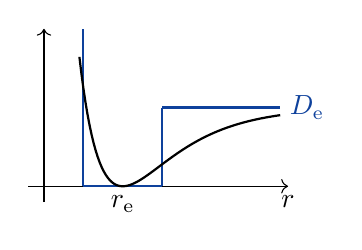
\begin{tikzpicture}[scale=1.0]
        % axis
        \draw[->] (-0.2,0) -- (3.1, 0);
        \draw[->] (0,-0.2) -- (0, 2);
        \node[below] at (3.1,0) {$r$};
        % \fill[lightgray] (-2,0) rectangle (0,3);
        % \fill[lightgray] (0,0) rectangle (3,2);
        % % potential
    
        \draw[thick,fudanBlue] (0.5,0) -- (0.5,2);
        \draw[thick,fudanBlue] (0.5,0) -- (1.5,0);
        \draw[thick,fudanBlue] (1.5,0) -- (1.5,1);
        \draw[thick,fudanBlue] (1.5,1) -- (3.0,1);
        
        % \node[below] at (3,0) {$l$};
        % functions
        \draw[domain=0.45:3,thick,samples=100] plot (\x,{(1 - exp(-1.5* (\x - 1)))^2});
        \node[below] at (1.0,0) {$r_{\mathrm e}$};
        \node[right,fudanBlue] at (3.0,1) {$D_{\mathrm e}$};
    
    \end{tikzpicture}
    \caption{分子间势能与半无限深势垒}
\end{figure}
这个半无限深的模型体系有什么用呢?可以类比化学键的行为。以氢气为例,
\begin{align}
    \text{键能} \quad &D_{\mathrm e} = \SI{4.74}{\electronvolt}\\
    \text{零点能} \quad &\SI{0.26}{\electronvolt}\\
    \text{平衡位置} \quad &r_{\mathrm e} = \SI{0.7414}{\angstrom}
\end{align}把氢气用这个半无限深势阱描述,其中单位换算为
\begin{align}
    & m = \SI{1.673E-27}{\kilo\gram}, \quad \mu = \frac{m}2, \\
    & \hbar = \SI{1.055E-34}{\joule\second},\\
    & \SI{1}{\electronvolt} = \SI{1.602E-19}{\joule},
\end{align}
这里的 $\mu$ 是氢分子的折合质量,满足
\begin{align}
    \frac1\mu = \frac1{m_{\mathrm H}} + \frac1{m_{\mathrm H}}, 
\end{align}
代入数据,得到
\begin{align}
    z_0 &= \frac{l}{\hbar} \sqrt{2 m V_0} \notag\\
    &= \frac{\SI{0.5E-10}{\metre}}{\SI{1.055E-34}{\joule\second}} \sqrt{
        \SI{1.673E-27}{\kilo\gram} \times 
        \SI{4.74}{\electronvolt} \times
        \SI{1.602E-19}{\joule\per\electronvolt}
    } \notag\\
    &\approx 23.89 \approx 7.6 \pi,
\end{align}
当 $z_0$ 很大时,$z_1$ 接近于 $\pi$,也就是接近于无限深势阱的 $z_1$。

应用量子化条件,得到零点能
\begin{equation}
    E_1 = \frac{\hbar^2\pi^2}{2ml^2} = \SI{0.04}{\electronvolt},
\end{equation}
求解出来发现这个模型并不能很好描述化学键。

\chat{%
氢气分子在平衡位置附近是连续的,目前这里的阶跃势能是有碍于正确描述零点能的。很自然的想法是用抛物线势能描述势能,本周主要的内容便是量子谐振子。
}
%2022-10-10 08:32:51  Wenbin Fan @FDU
\chapter{量子谐振子}
% 【图】【二次函数】
\begin{figure}[tp]\centering
    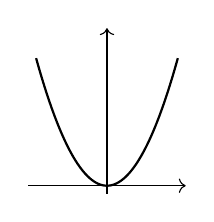
\begin{tikzpicture}[scale=0.5]
        % axis
        \draw[->] (-2,0) -- (2, 0);
        \draw[->] (0,-0.2) -- (0, 4);
        % \node[below] at (3.1,0) {$r$};
    
        \draw[domain=-1.8:1.8,thick,samples=100] plot (\x,{\x*\x});
    
    \end{tikzpicture}
    \caption{抛物势}
\end{figure}
势函数
\begin{align}
    V(x) = a x^2,
\end{align}
称为\boldtext{抛物线} parabolic 势函数。
% 【刚才是???,有什么不一样】
% 【求得波函数???】
\chat{%
刚才通过化学键的定义,引出了量子体系。换个角度,量子谐振子有什么不同?我们能从公设推知微观粒子的行为,前提是确立状态方程、求解波函数,其中状态方程中最重要的系统依赖项就是势函数。上周的一维量子体系是简单的量子状态,要么为 0,要么是有限值,所有的复杂情况都来自边界条件,由边条件可以推知所有的物理。

今天要求解的量子体系,势函数是显式地依赖于坐标的。求解之前有个问题,$a$ 表示的是什么物理量。
}
\begin{figure}[tp]\centering
    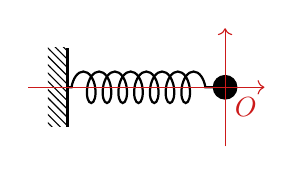
\begin{tikzpicture}[scale=0.5]
        % % axis
        % \draw[->] (-2,0) -- (2, 0);
        % \draw[->] (0,-0.2) -- (0, 4);
        % % \node[below] at (3.1,0) {$r$};
    
        \fill [pattern = north west lines] (-0.5,0) rectangle (0,2);
        \draw[thick] (0,0) -- (0,2);
        \draw[
        decoration={
            coil,
            segment length = 2mm,
            amplitude = 2mm,
            aspect = 0.5,
            post length = 1mm,
            pre length = 0.5mm},
        decorate, thick] (0,1) -- (4,1);
        \draw[fill] (4,1) circle (0.3);
    
        % \draw[domain=-1.8:1.8,thick,samples=100] plot (\x,{\x*\x});
    
        % axis
        \draw[->, fudanRed] (-1,1) -- (5, 1);
        \draw[->, fudanRed] (4,-0.5) -- (4, 2.5);
        \node[right,fudanRed] at (4,0.5) {$O$};
    
    \end{tikzpicture}
    \caption{弹簧模型}
    \end{figure}
回顾胡克定理,
% 【图,左边是墙,水平连接弹簧】,
以平衡构型建立坐标系 $O$,弹簧受到的力为 $F = -kx$,$k$ 是弹簧的劲度系数 stiffness coefficient。由牛顿力学定律
\begin{align}
    F = ma = m \pdv[2]{x}{t} = -k x
\end{align}
得到偏微分方程
\begin{align}
    \pdv[2]{x}{t} = - \frac km x,
\end{align}
很容易得到运动轨迹
\begin{align}
    x(t) = A \sin(\omega t + \delta),
\end{align}
其中 $\omega = \sqrt{\frac{k}m}$ 是振子的角频率,是体系内禀的量,$A,\delta$ 是振幅和相位,与初态有关。另外我们知道,
\begin{align}
    F(x) = -\frac{\partial V(x)}{\partial x}, 
\end{align}
解出来势能
\begin{align}
    V(x) = \int -F(x)\,\dd x = \int kx \, \dd x = \frac12 k x^2 + V_0,
\end{align}
令参考势能 $V_0 = 0$,那么势能
\begin{eqnarray}
    V(x) = \frac 12 kx^2 = \frac 12 m\omega^2 x^2.
\end{eqnarray}
由此,得到了 $a$ 的物理含义。

量子谐振子的哈密顿量,
\begin{align}
    \hat H(x) = -\frac{\hbar^2}{2m} \pdv[2]{x} + \frac 12 m\omega^2 x^2,
\end{align}
定态薛定谔方程就可以写为
\begin{align}
    -\frac{\hbar^2}{2m} \pdv[2]{\psi}{x} + \frac 12 m\omega^2 x^2 \psi = E\psi,
    \label{eq:harm_seq_original}
\end{align}
看起来有点太复杂了,能否简化其中的常数?

\section{方程简化}

两边同除以 $-\frac{\hbar^2}{2m}$,
\begin{align}
    \pdv[2]{\psi}{x} - \frac{m^2\omega^2 x^2}{\hbar^2} \psi = \frac{-2mE}{\hbar^2}\psi,
\end{align}
归并到左边,有
\begin{align}
    \pdv[2]{\psi(x)}{x} + \left(
        \frac{2mE}{\hbar^2} - \frac{m^2\omega^2}{\hbar^2} x^2
    \right) \psi = 0,
\end{align}
设 $a = \frac{m\omega}{\hbar}$,有
\begin{align}
    \pdv[2]{\psi(x)}{x} + \left(
        \frac{2mE}{\hbar^2} - a^2 x^2
    \right) \psi = 0,
    \label{eq:harm_seq_a}
\end{align}
利用函数变量代换的规则,定义新的变量 $y = kx$,即 $x = \frac 1k y$,那么波函数 $\psi(x) = \psi(y)$,利用链式法则
\begin{align}
    &\pdv{\psi(x)}{x} = \pdv{\psi(y)}{y} \pdv yx = k \pdv{\psi(y)} {y},
    &\pdv[2]{\psi(x)}{x} = k^2 \pdv[2]{\psi(y)}{y},
\end{align}
代回薛定谔方程 \eqref{eq:harm_seq_a}
\begin{align}
    k^2 \pdv[2]{\psi(y)}{y} + \left(
        \frac{2mE}{\hbar^2} - \frac{a^2}{k^2} y^2
    \right) \psi(y) &= 0 \\
    \pdv[2]{\psi(y)}{y} + \left(
        \frac{2mE}{\hbar^2} - \frac{a^2}{k^4} y^2
    \right) \psi(y) &= 0
\end{align}
之前对 $k$ 是没有要求的,这里为了化简系数,令 $y^2$ 项前的系数为 1,设 $k^4 = a^2$,有 $y = \sqrt a x$,得到
\begin{align}
    \pdv[2]{\psi(y)}{y} + \left(
        \frac{2mE}{\hbar^2} - y^2
    \right) \psi(y) &= 0
\end{align}
其中还有一项
\begin{eqnarray}
    \frac{2mE}{a\hbar^2} = \frac{2mE}{m\omega\hbar^2} = \frac{2E}{\hbar\omega} = \lambda,
\end{eqnarray}
有
\begin{align}
    \pdv[2]{\psi(y)}{y} + (\lambda - y^2) \psi(y) = 0,
    \label{eq:harm_seq_lambda_y}
\end{align}
% 【标记了原始 Seq (1),上式为 2】
这种偏微分方程叫做变系数二阶常微分方程,这就是谐振子的\boldtext{标准方程}。

\chat{%
这个方程有很多种解法,已经被研究得很透彻了,这里讲一个标准做法。

为了求解,有必要对这个微分方程的轮廓有认知。
首先遇到的问题,是否有对称性,或者说具有什么样的对称性?
}
% 第二节
% 【】
\section{波函数的对称性}
由势函数可知
\begin{align}
    V(x) = V(-x),
\end{align}
因此对应的本征波函数 $\psi(x)$ 即 $\psi(y)$ 有确定的宇称,那么波函数要么是奇函数 $\psi(x) = -\psi(-x)$、要么是偶函数 $\psi(x) = \psi(-x)$。
\homework{\textbf{4.1} ~ (a) 对于一维的宇称算符
\begin{align}
    \hat\Pi \psi(x) = \psi(x),
\end{align}
证明 $\hat \Pi$ 是 Hermit 算符,

(b) 证明,当 $V(x) = V(-x)$ 时,$[\hat H, \hat \Pi] = 0$,

(c) 考察 $[\hat T, \hat V]$ 是否为 0,并进一步考察 $[\hat T, \hat H]$、$[\hat V, \hat H]$ 是否为 0。
}

\section{无穷远处的渐进性质}
为了求解方程,先尝试求极限情况。

当 $x \rightarrow \pm \infty$,即 $y \rightarrow \pm \infty$,$y^2 \gg \lambda$,有
\begin{align}
    \frac{\partial^2 \varphi(y)}{\partial y^2}+\left(\lambda-y^2\right) \varphi(y)=0 \Rightarrow \frac{\partial^2 \varphi(y)}{\partial y^2}-y^2 \varphi(y)=0,
\end{align}

设 $\psi(y) = \ee^{sy}$,它非奇非偶,不满足。换一种波函数,设 $\psi(y) = \ee^{sy^2}$,如果要满足品优波函数的性质,$s<0$,所以直接设为 $\psi(y) = \ee^{-sy^2} (s>0)$,求导有
\begin{align}
    &\frac{\partial}{\partial y} \ee^{-sy^2} = -2sy \, \ee^{-sy^2}, \\
    &\pdv[2]{\psi(y)}{y} = -2 s\, \ee^{-s y^2} + 4 s^2 y^2 \ee^{-s y^2},
\end{align}
\begin{lstlisting}
    D[Exp[-s y^2], y]
    D[Exp[-s y^2], {y, 2}]
    >> -2 E^(-s y^2) s y
    >> -2 E^(-s y^2) s + 4 E^(-s y^2) s^2 y^2
    \end{lstlisting}
代回原式有
\begin{align}
    4s^2 y^2 \, \ee^{-sy^2} - y^2 \ee^{-sy^2} - 2 s \ee^{-sy^2} &= 0 \\
    4s^2 y^2 \, \ee^{-sy^2} - y^2 \ee^{-sy^2} &= 0, \\
    4 s^2 & = 1,
\end{align}
解得 $s = \frac12$。得到了波函数在无穷远处的渐进性为,
\begin{equation}
    \psi(y) |_{y \rightarrow \pm\infty} = \ee^{-y^2/2}.
\end{equation}
\section{引入 Hermite 方程}
波函数可以写为
\begin{equation}
    \psi(y) = f(y) \ee^{-y^2/2},
\end{equation}
问题转化成了求解 $f(y)$。

当$y\rightarrow\pm\infty$ 时,$f(y) \rightarrow A$ 常数,才能确保 $\psi$ 的渐进行为。重新求导 
% % []
% \begin{align}
%     \pdv[2]{\psi(y)}{y} + (\lambda - y^2) \psi(y) = 0, 
% \end{align}
% []
% \begin{align}
%     \psi(y) = f(y) \, \ee^{-y^2/2},
% \end{align}
% $f(y)$ 为待求解函数,当 $y \rightarrow \pm\infty$ 时,$f(y) = A$,$\psi(y) \rightarrow \ee^{-y^2/2}$,
% 偏导为
\begin{align}
    &\frac{\partial \varphi(y)}{\partial y}=\frac{\partial f(y) e^{-y^2/2}}{\partial y}=f'(y) e^{-y^2 / 2}-y e^{-y^2 / 2} f(y) \\
    &\frac{\partial^2 \varphi(y)}{\partial y^2}=f^{\prime \prime}(y) e^{-y^2 / 2}-2 y e^{-y^2 / 2} f^{\prime}(y)+\left(y^2-1\right) e^{-y^2 / 2} f(y)
\end{align}
\begin{lstlisting}
Clear[f, y]
D[f[y] Exp[-y^2/2], y] // Simplify
D[f[y] Exp[-y^2/2], {y, 2}] // Simplify
>> E^(-(y^2/2)) (-y f[y] + Derivative[1][f][y])
>> E^(-(y^2/2)) 
    ((-1 + y^2) f[y] - 2 y Derivative[1][f][y] 
    + (f^\[Prime]\[Prime])[y])
\end{lstlisting}
代回到 \eqref{eq:harm_seq_lambda_y} 中,
\begin{align}
    f^{\prime \prime}(y) e^{-y^2 / 2}-2 y e^{-y^2 / 2} f^{\prime}(y)+(\lambda-1) e^{-y^2 / 2} f(y)=0
\end{align}
% [][]Hermite 方程。
% 【】【】【4式】
稍微化简即可得另一个变系数常微分方程,
\begin{align}
    f''(y) - 2y f'(y) + (\lambda - 1) f(y) = 0, 
    \label{eq:harm_lambda_y_simp} %eq4 in course
\end{align}
称其为 Hermite 方程。

\chat{%
回到初始薛定谔方程,引入变量代换可以得到变系数常微分方程。很自然的问题是,
为什么我们要做如此多步的方程演化?换句话说,我们可否直接求 \eqref{eq:harm_seq_original} 或 \eqref{eq:harm_seq_lambda_y}?为什么变换之后求解更方便?

物化里面可能讲过,下面将会用到幂级数展开法。
}

\section{幂级数展开法}
将函数作级数展开,
\begin{align}
    &f(y) = \sum_{n=0}^\infty c_n y^n = c_0 + c_1 y + c_2 y^2 + \cdots,\\
    &f'(y) = \sum_{n=1}^\infty n c_n y^{n-1}, \\
    &f''(y) = \sum_{n=2}^\infty n(n-1) c_n y^{n-2},
\end{align}
将幂级数代回 \eqref{eq:harm_lambda_y_simp},
% 【label 5,6】
% 代回【?】,
导数的下限取值从 1、2 开始,写成从 0 开始是完全一样的,
\begin{align}
    & \sum_{n=2}^{\infty} n(n-1) c_n y^{n-2}-2 y \sum_{n=1}^{\infty} n c_n y^{n-1}+(\lambda-1) \sum_{n=0}^{\infty} c_n y^n \\
    =& \sum_{n=2}^{\infty} n(n-1) c_n y^{n-2}-\sum_{n=1}^{\infty} 2 n c_n y^n+\sum_{n=0}^{\infty}(\lambda-1) c_n y^n \\
    =& \sum_{n=2}^{\infty} n(n-1) c_n y^{n-2}-\sum_{n=0}^{\infty}(2 n-\lambda+1) c_n y^n
\end{align}
设 $m=n-2$,有
\begin{align}
    \sum_{m=0}^{\infty}(m+2)(m+1) c_{m+2} y^m-\sum_{n=0}^{\infty}(2 n-\lambda+1) c_n y^n
\end{align}
设 $n=m$,再把变量换回 $n$,有
\begin{align}
    &\sum_{n=0}^{\infty}(n+2)(n+1) c_{n+2} y^n-\sum_{n=0}^{\infty}(2 n-\lambda+1) c_n y^n \\
    ={}&\sum_{n=0}^{\infty}\left[(n+2)(n+1) c_{n+2}-(2 n-\lambda+1) c_n\right] y^n = 0, 
\end{align}
上式为 0,意味着其中每一项都要相等,
\begin{align}
    (n+2)(n+1) c_{n+2} = (2n - \lambda + 1)c_n,
\end{align}
便得到了双间隔的递推公式
\begin{align}
    c_{n+2} = \frac{2n - \lambda + 1}{(n+2)(n+1)} c_n, \quad n = 0, 1,2, \cdots,
\end{align}

做两件事,(1) 从 $c_0$ 开始推,
\begin{align}
    &n =0, \quad c_2 = \frac{1-\lambda}{2\times 1} c_0, \\
    &n=2, \quad c_4 = \frac{4 + 1 - \lambda}{4\times 3} c_2 = \frac{(1-\lambda)(4+1 - \lambda)}{4\times3\times2\times1} c_0, \\
    &n = 4, \quad c_6 = \frac{(1-\lambda) (4+1-\lambda) (8+1-\lambda)}{6!} c_0,
\end{align}
\begin{lstlisting}
(* 递归求解系数 *)
    Clear[c];
c[n_] := (2 (n - 2) - \[Lambda] + 1)/(n (n - 1)) c[n - 2]
c[0] := c0;
Table[c[2 i], {i, 1, 5}]
>> {1/2 c0 (1 - \[Lambda]), 
    1/24 c0 (1 - \[Lambda]) (5 - \[Lambda]), 
    1/720 c0 (1 - \[Lambda]) (5 - \[Lambda]) (9 - \[Lambda]), (
    c0 (1 - \[Lambda]) (5 - \[Lambda]) (9 - \[Lambda]) (13 - \
\[Lambda]))/40320, (1/3628800)
    c0 (1 - \[Lambda]) (5 - \[Lambda]) (9 - \[Lambda]) (13 - \[Lambda]) \
(17 - \[Lambda])}
\end{lstlisting}
% 于是
相当于给出
\begin{multline}
    f_0(y) = 
    \left[
        1 + \frac{1-\lambda}{2!} y^2 + 
        \frac{(1-\lambda) (4+1 - \lambda)}{4!} y^4 \right. \\
        \left.+ \frac{(1-\lambda) (4+1-\lambda) (8+1-\lambda)}{6!} y^6 + \cdots
    \right] c_0,
\end{multline}

(2) 从 $c_1$ 开始递推,不再具体讲了,最后结果是
\begin{multline}
    f_1(y) = \left[y + \frac{2+1 - \lambda} {3!} y^3 + \frac{(2+1-\lambda)(6+1 -\lambda)}{5!} y^5 \right. \\
    \left.+ \frac{(2+1-\lambda)(6+1-\lambda)(10+1-\lambda)}{7!} y^7
    + \cdots \right] c_1,
\end{multline}

我们利用幂级数展开,求解得到了奇数和偶数情况。那么合并到一起,
\begin{align}
    f(y) = c_0 f_0(y) + c_1 f_1(y),
\end{align}
于是 Hermite 方程 \eqref{eq:harm_lambda_y_simp} 的通解为上式子。
% 【4 是 f prime prime (y) - 2 ...】
\chat{%
前面讲过,势能是偶函数,那么波函数也必然有某种确定的宇称,
要么是偶函数 $f_0$,要么是奇函数 $f_1$,不可能是线性组合,二者单独都具有宇称,一旦组合起来就破坏的宇称。
}

% 下午的课

% 上午做了些方程的简化、讨论了渐进行为、做了幂级数的展开,得到双间隔的递推公式。
% 宇称,是名词,为何作形容词?% 2022-10-10 13:34:55  Wenbin Fan @FDU
\courseTime{3 of 4, Oct 10}
考察系数在无穷大时的行为,上下同除 $n^2$,将衰减较快二次项扔掉,即
\begin{align}
    \frac{c_{n+1}}{c_n} = \frac{2n - \lambda + 1} { (n+2) (n+1)} = \frac{ \frac{2}{n} + \frac{-\lambda+1}{n^2} } { \left(1+\frac 2n\right) \left(1+\frac1n\right) } \rightarrow \frac 2n,
\end{align}
注意到指数函数的幂级数展开,
\begin{align}
    \exp y^2 = 1 + \frac{y^2}{1!} + \frac{y^4}{2!} + \cdots + \frac{y^n}{\left(\frac n2\right)!} + \frac{y^{n+2}}{\left(\frac n2 +1\right)!} + \cdots,
\end{align}
相邻系数的比例关系,
\begin{align}
    \frac{c_{n+2}}{c_n} = \frac{\left(\frac n2\right)!} {\left(\frac n2 + 1\right)!} = \frac1{\frac n2 +1} \rightarrow \frac 2n
\end{align}
当 $y\rightarrow\infty$ 时,$f_0(y)$、$f_1(y)$ 与 $\exp y^2$ 的性质主要取决于 $n$ 较大时的高次项,即当 $n$ 很大时,$\exp y^2$ 与 $f(y)$ 有相同的性质,所以二者在 $y\rightarrow\infty$ 时有相同的渐进性为,
\begin{align}
    \psi(y) = f(y) \ee^{-y^2/2} |_{y\rightarrow \infty} = \exp y^2 \exp \left(-\frac{y^2}2\right) = \exp \frac{y^2}2 \rightarrow \infty.
\end{align}
这个波函数必须满足的品优性质。品优波函数的有限性,限制 $f(y)$ 必须在某一项终止,使它成为多项式。具体来说,品优波函数的限制对 Hermite 方程
\eqref{eq:harm_lambda_y_simp}
% $f''(y) - 2 y f'(y) + (\lambda -1) f(y) = 0$
中的任意实数 $\lambda$ 提出了量子化的条件。

如果波函数有限,必须在某一项停止。只要分子上 $2n - \lambda +1$ 任何一项为 0,后面的项也全部为 0。由此解出
\begin{align}
    \lambda = 2n +1, \quad n = 0, 1, 2, 3, \cdots
\end{align}
代入 $\lambda$ 的设定,得到
\begin{align}
    \frac{2E}{\hbar\omega} = 2n+1  \ \Rightarrow \ E = \left(n+\frac12\right)\hbar\omega,
\end{align}
特别地,当 $n=0$ 时,
\begin{align}
    E_0 = \frac12\hbar \omega,
\end{align}

求解中最重要的简化步骤,是对方程 \eqref{eq:harm_seq_lambda_y} 的渐进行为思考。那么回答之前的问题,为什么要做如此多步的推导?这是个开放式的问题。

\homework{
    \textbf{4.2} ~  对于谐振子标准方程 \eqref{eq:harm_seq_lambda_y},做幂级数展开,给出系数的递推公式,并讨论能否从中得到量子化条件。

    \textbf{4.3} ~  针对谐振子 Hermite 方程 \eqref{eq:harm_lambda_y_simp},引入复变量 $\rho = y^2$,将 Hermite 方程演化为 Kummer's 微分方程,并对它做幂级数展开、给出系数的递推公式和量子化条件。
}

已经求出了量子化条件,那么此时的量子谐振子模型有什么特殊或不一样的意义、物理行为?下面做更多有趣的分析。

\section{量子化条件的分析}

量子化条件决定了量子特征,下面分析零点能。

% \subsection{零点能}

当 $n=0$ 时,只有 $c_0$ 这一项,波函数是高斯展宽。

氢分子势能面上解离的问题,再用谐振子模型重新算一次。
$\mathrm H_2$ 的劲度系数 $k = \SI{1.3E3}{\newton\per\metre}$,得到 $\omega = \sqrt{\frac km} = \SI{8.2E14}{\hertz}$,则
\begin{eqnarray}
    E_0 = \frac 12 \hbar \omega = \SI{0.27}{\electronvolt}, 
\end{eqnarray}
这与实验值是非常相符的。换句话说,对于键能比较强的键,谐振子能给出比较准确的零点能,现在广泛采用的也是谐振子模型。

\section{本征函数}
已经得到
\begin{align}
    \psi(y) = A f(y) \ee^{-y^2/2},
\end{align}
其中 $A$ 是归一化系数,也得到了 $f_0$、$f_1$ 和量子化条件,那么可以等价地给出
\begin{align}
    &\phi_0^n (y) = A f_0^n (y) \ee^{-y^2/2}, \quad\text{偶函数}\\
    &\phi_1^n (y) = A f_1^n (y) \ee^{-y^2/2}, \quad\text{奇函数}
\end{align}
现在波函数还是非常复杂的。

为了简化多项式,取 $c_n = 2^n$,利用递推公式
\begin{align}
    c_{k+2} = \frac{2k - 2n}{(k+2)(k+1)}c_k. 
\end{align}
本来是利用 $c_0$ 从小到大推进,所以很容易得到量子化条件等,但弊端是难以写出通式。现在我们反着来做,假设截断后的最高一项是 $2^n$,再从大到小推导其它系数,推导得到
\begin{align}
    H_n(y) = \sum_{m=0}^M \frac{(-1)^m n!}{m! (n-2m)!} (2y)^{n-2m}, 
\end{align}
其中 $m$ 为求和指标,$M$ 是最大值,
\begin{align}
    M = \begin{cases}
        \frac n2, \quad n = 0, 2, 4, \cdots, \\
        \frac{n-1}2, \quad n=1,3,5,\cdots,
    \end{cases}
\end{align}
那么通过反推,可以使我们的解变成很简单的形式。
该式称为 $n$ 阶 \boldtext{Hermite 多项式},
\begin{align}
    H_n(y) = (-1)^n H_n(y), \label{eq:nth_hermitian_poly}
\end{align}
写出前 $n$ 阶 Hermite 多项式,
\begin{align}
    &H_0 (y) = 1, \\
    &H_1(y) = 2y,\\
    &H_2(y) = 4 y^2 - 2, \\
    &H_3(y) = 8 y^2 - 12 y, \\
    &H_4(y) = 16 y^4 - 48 y^2 + 12, 
\end{align}
\begin{lstlisting}
(* 厄米多项式 *)
Table[HermiteH[i, y], {i, 0, 5}]
>> {1, 2 y, -2 + 4 y^2, -12 y + 8 y^3, 12 - 48 y^2 + 16 y^4, 
120 y - 160 y^3 + 32 y^5}
\end{lstlisting}
我们约束了 Hermite 多项式是有限的,并且给定了最大的值。

这种从大到小的推导,可以与从小到大的推导做一一对应,
\begin{alignat}{2}
    &f_0^0(y) = 1 &&=H_0(y),\\
    &f_0^2(y) = 1 - 2y^2  && = - \frac12 H_2(y), \\
    &f_0^4(y) = 1- 4 y^2 + \frac43 y^4 && = 12 H_4(y),
\end{alignat}
二者相差倍数关系,这个倍数可以包括在归一化系数中,所以二者是完全等价的。

% 2022-10-10 14:15:02  Wenbin Fan @FDU
% ---
我们已经通过 $M$ 包括了奇数和偶数两种情况,波函数
\begin{align}
    &\psi(y) = A f(x) \ee^{-y^2/2}, \\
    &\psi_n(y) = A_n H_n (y) \ee^{-y^2/2}, \quad n=0,1,2,\cdots, \\
    & y = ax = \sqrt{\frac{m\omega}{\hbar}} x, \quad a^2 = \frac{m\omega}\hbar,
\end{align}
\homework{\textbf{4.5} ~  
请证明
\begin{align}
    A_n = \left(\frac{m\omega}{\pi\hbar}\right)^{1/4} \frac1 {\sqrt{2^n n!}},
\end{align}
提示,可利用 Hermite 多项式生成函数
\begin{align}
    S(x,r) = \ee^{2xr -r^2} = \sum_{n=0}^{\infty} H_n(x) \frac{r^n}{n!}, 
\end{align}
来讨论,这里可参考顾樵《量子力学》P208---211。
% 电子图书见 elearning。

体系的基态\begin{align}
    \psi_0(x) &= \left(\frac{m\omega}{\pi\hbar}\right)^{1/4} \exp \left(- \frac12 \frac{m\omega}{\hbar} x^2\right)\\
    &=\left(\frac a{\sqrt{\pi}}\right)^{1/2} \exp\left(-\frac12 a^2 x^2\right),\\
    \psi_1(x) &= a \left(\frac{2a}{\sqrt{\pi}}\right)^{1/2} x \exp \left(-\frac12 a^2 x^2\right),
\end{align}
}
% 把顾的书放上去

% 2022-10-10 14:29:36  Wenbin Fan @FDU
% 休息回来
由此知道了基态形式。画出图来,基态是个高斯函数,偶函数,更高阶的情况也可以依次画出。$n=1$ 有节点,$n=2$ 有 2 个节点,那么 $n$ 有 $n$ 个节点。
\begin{lstlisting}
(* 波函数可视化 *)
m = 1; \[Omega] = 1; \[HBar] = 1;
\[Psi][n_, x_] := ((m \[Omega])/(\[Pi] \[HBar]))^(1/4) 1/Sqrt[2^n n!]
HermiteH[n, x] Exp[-1/2 (m \[Omega])/\[HBar] x^2];
Plot[Table[\[Psi][i, x], {i, 0, 3}] // Evaluate, {x, -5, 5}]
\end{lstlisting}
\homework{
    \textbf{4.6} ~  证明谐振子 $n=0,1$ 两种情况下,不确定原理成立,计算 $(\Delta x)_n^2 (\Delta p)_n^2$ 在 $n=0,1$ 的值。

    提示,
    \begin{align}
        &(\Delta x)_n^2 = \langle \psi_n | \hat x^2 | \psi_n \rangle - \langle \psi_n | \hat x | \psi_n \rangle^2, \\
        &(\Delta p)_n^2 = \langle \psi_n | \hat p^2 | \psi_n \rangle - \langle \psi_n | \hat p | \psi_n \rangle^2,
    \end{align}
}

\section{概率密度}

问题1,经典的谐振子在什么位置出现的概率最大?

这里不方便画图,直接给大家结果,密度分布为
\begin{align}
    &\rho(x) = \frac1{\pi\sqrt{A^2 - x^2}}, \\
    &\rho(0) = \frac 1{\pi A}, \quad \rho(\pm A) = +\infty
\end{align}
% 实际上推导需要用到关系式,用到胡克定律坐标和时间的关系,又知道
% \begin{align}
%     \rho(x) \dd x = \dd t / \frac{\tau}2,
% \end{align}
因为两端速度为 0,那么概率最大,最低点速度最大,概率相对小一些。
\begin{figure}[tp]\centering
    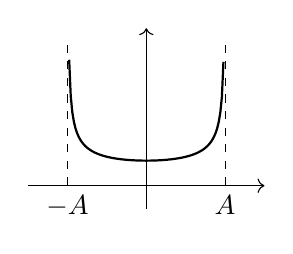
\begin{tikzpicture}[scale=1.0]
        % axis
        \draw[->] (-1.5,0) -- (1.5, 0);
        \draw[->] (0,-0.3) -- (0, 2);
    
        % % \node[below] at (3.1,0) {$r$};
    
        \draw[domain=-0.98:0.98
        ,thick,samples=100] plot (\x,{1/(pi*sqrt(1-\x*\x))});
    
        \draw[dashed] (-1, 0) -- (-1, 1.8);
        \draw[dashed] (1, 0) -- (1, 1.8);
        \node[below] at (-1,0) {$-A$};
        \node[below] at (1,0) {$A$};
    
    \end{tikzpicture}
    \caption{经典谐振子的概率密度}
\end{figure}
\suppInfo{经典谐振子的概率密度}{
从牛顿方程可以解得谐振子的轨迹
\begin{equation}
    x = A \sin (\omega t + \varphi),
\end{equation}
坐标方向的概率相当于 $\rho(x) = \frac{\dd t}{\dd x}$,反解出
\begin{equation}
    t = \frac{-\arcsin\frac{x}{A}-\varphi
   +\pi }{\omega }
\end{equation}
求导得到
\begin{eqnarray}
    \frac{\dd t}{\dd x} = -\frac{1}{\omega  \sqrt{A^2-x^2}},
\end{eqnarray}
归一化后即可得到密度分布。
}

\subsection{量子谐振子的概率密度}

经典图像中,在超出 $|A|$ 的区域中,概率是为 0 的,所以有了经典振幅的概念。

量子谐振子的波函数为
\begin{align}
    \psi_n(y) = A_n H_n(y) \exp^{-y^2/2}, \quad n=0,1,2,\cdots,
\end{align}
概率密度为模方,
\begin{align}
    |\psi_n(y)|^2 = |A_n|^2 \ee^{-y^2} |H_n (y)|^2 
    = \frac{a}{2^n n! \sqrt{\pi}} \ee^{-y^2} |H_n(y)|^2,
\end{align}

引入经典禁区 (classical restricted area) 的概念,谐振子的势能是 $V(x) = \frac 12 m\omega^2 x^2$,量子化的条件
\begin{align}
    \hbar\omega \left(n+\frac12\right) = \frac12 m\omega^2 \bar A_n^2,
\end{align}
其中 $\bar A_n$ 为量子振幅,那么
\begin{align}
    \bar A_n = \sqrt{\frac{2\hbar}{m\omega} \left(n+\frac12\right)} = \frac1a \sqrt{2n+1},
\end{align}
利用 $y=ax$,那么
\begin{align}
    \bar a_n = a \bar A_n = \sqrt{2n+1}
\end{align}
为无量纲振幅。

对于基态,
\begin{align}
    |\psi_0(y)|^2 = \frac{a}{\sqrt{\pi}} \ee^{-y^2},
\end{align}
依然是个高斯展宽,经典禁区的概率
\begin{align}
    Q_0 &= \int_{-\infty}^{-\bar A_n} |\psi_0(x)|^2 \dd x + \int_{\bar A_n}^{\infty} |\psi_0(x)|^2 \dd x \\
    &= 2 \int_{-\infty}^{-\bar A_n} |\psi_0(x)|^2 \dd x \\
    &= \frac{2}{\sqrt{\pi}} \int_{\bar a_0}^{\infty} \ee^{-y^2}\,\dd y \\
    &= \mathrm{erfc}(y),
\end{align}
% II $ x=\bar a_0 = 1$, 
同理计算出 $Q_0 = 0.157$, $Q_1 = 0.112$, $Q_2 = 0.095$, $\cdots$, $Q_{10} = 0.060$, $\cdots$。
\begin{lstlisting}
Clear["Global`*"]
\[Psi][n_, x_] := ((m \[Omega])/(\[Pi] \[HBar]))^(1/4) 1/Sqrt[2^n n!]
    HermiteH[n, 
    Sqrt[(m \[Omega])/\[HBar]] x] Exp[-1/2 (m \[Omega])/\[HBar] x^2];
n = 10;
Integrate[
    2 \[Psi][n, 
    x]^2, {x, -Infinity, -Sqrt[(2 \[HBar])/(m \[Omega]) (n + 1/2)]}, 
    Assumptions -> {m > 0, \[Omega] > 0, \[HBar] > 0}]
N[%]
>> (19634522823 Sqrt[21/\[Pi]])/(640 E^21) + Erfc[Sqrt[21]]
>> 0.0601438
\end{lstlisting}

当 $n$ 较大时,与量子情况较为接近。
\begin{lstlisting}
(* 画图,n 较大时的密度分布 *)
m = 1; \[Omega] = 1; \[HBar] = 1;
\[Psi][n_, x_] := ((m \[Omega])/(\[Pi] \[HBar]))^(1/4) 1/Sqrt[2^n n!]
    HermiteH[n, Sqrt[(m \[Omega])/\[HBar]] x] 
    Exp[-1/2 (m \[Omega])/\[HBar] x^2];
n = 10;
Plot[
    {\[Psi][n, x]^2, 
    (Pi Sqrt[(2 \[HBar])/(m \[Omega]) (n + 1/2) - x^2])^-1}, 
    {x, -6, 6}]
\end{lstlisting}


\section{复习}
\courseTime{Oct 17, 2022 \\ 5th}
\chat{%
上周被关了多久(笑)?上周是第一次线上上课,讲课特别不舒服。

上周讲了量子谐振子。这个科学问题来自氢分子的势能面,不管是定性还是定量,都要跟分子间相互作用打交道,包括弱相互作用、强相关作用等等。

在解离势能面最低点是平衡构型,这点能量与解离能量的差是解离能 $D_{\mathrm e}$。氢分子的势能也可以用单侧无限深势阱描述,类似束缚态。由品优波函数的条件,得到束缚态的超越方程 $\cot z = - \sqrt{\left(\frac{z_i}z\right)^2 - 1}$,解之得离散化的能量 $\{z_i\}$。这个模型预测零点能,误差极大。所以我们知道,想要预测整体性质——零点能,需要在平衡位置接近真实势能,特别是平衡位置的曲率。

从平衡位置做泰勒展开,那么得到了抛物势 $V(x) = \frac12 m \omega x^2$,即谐振子模型。利用品优条件求解它,得到了量子化的解。最重要的品优条件是无穷远处不能发散,由此得到了 Hermite 方程、间隔的递推公式,其中的发散项让我们必须在某项截断它。最终解得零点能 $E_i = \hbar\omega\left(n + \frac12\right)$。相比于单侧无限深势阱,这个的势能形状更符合氢气的解离曲线。值得关注的是,能级间隔是相等的 $\Delta E = \hbar\omega$,当氢分子偏离平衡位置时,非谐振效应体现出来,只能描述低振动级别的振动态,这是谐振子模型无法描述的,而单侧无限深势阱区分了束缚态和解离态。
}

我们引入更符合真实的 Morse 势,其定义为
\begin{eqnarray}
    V(x) = D_{\mathrm e} \ee^{-a (r-r_\mathrm e)} ( \ee^{-a (r - r_\mathrm e)} - 2),
\end{eqnarray}
在平衡处 $r_\mathrm e$ 有最小值,在无穷远处为 0。Morse 势的薛定谔方程有解。
\begin{lstlisting}
(* 画出 Morse 势能的图 *)
Clear["Global`*"]
De = 1; \[Alpha] = 1; re = 1;
M[r_] := De (1 - Exp[-\[Alpha] (r - re)])^2
Plot[M[r], {r, 0, 5}]
\end{lstlisting}
\homework{\textbf{5.1} 比较谐振子与 Morse 势能函数,参考 JCP 1988, 88(7) 4535 ``The Morse oscillator in position space and phase space''}
\chat{%
越接近真实体系,薛定谔方程越难求解。从没有限制的自由粒子开始,到简单的势能(仅通过边界条件求解),到现在势能形状也接近真实物理。当势能复杂到无法解析求解时,便可以通过\textbf{数值}求解。
}
\homework{\textbf{5.1} (\emph{continued}) (选做)采用 Numerov 方法数值求解。见 Levin \emph{Quantum Chemistry} Sec 4.4 P70}

\chapter{粒子的转动与角动量}
\chat{%
为什么要学习转动,因为真实体系不止有平动,还有转动、振动等。

从基本公设出发,可以解薛定谔方程求出体系的波函数。对体系了解程度,在于波函数的精确程度,求解的困难程度在于势函数的复杂性。

前面解了那么多的体系,共同点是一维的。}

从一维拓展到二维,最简单的还是自由粒子,哈密顿算符
\begin{align}
    \hat H = -\frac{\hbar^2}{2m} \left(\pdv[2]{x} + \pdv[2]{y}\right),
\end{align}
那么薛定谔方程
\begin{align}
    \hat H \Psi(x,y) = E \Psi(x,y)
\end{align}
我们希望波函数可以分离变量,
\begin{align}
    \Psi(x,y) = X(x) Y(y), \label{eq:2dtrans_sepXY}
\end{align}
得到左右两边相互独立的式子,
\begin{align}
    \hat F(x) X(x) = \hat G(y) Y(y)
\end{align}
数学上可以证明上式等价于
\begin{align}
    &\hat F(x) X(x) = C, \\
    &\hat G(y) Y(y) = C. 
\end{align}

将 \eqref{eq:2dtrans_sepXY} 代回薛定谔方程,
\begin{align}
    -\frac{\hbar}{2m} \left(\pdv[2]x + \pdv[2]y\right) X(x) Y(y) &= E X(x) Y(y) \\
    -\frac{\hbar^2}{2m} Y(y) \pdv[2]x X(x) - \frac{\hbar^2}{2m} X(x) \pdv[2]y Y(y) &= E X(x) Y(y) \\
    -\underbrace{\frac{\hbar^2}{2m} \frac1{X(x)} \pdv[2]x X(x)}_{\text{只与 $x$ 有关}} - 
    \underbrace{\frac{\hbar^2}{2m} \frac1{Y(y)} \pdv[2]y Y(y)}_{\text{只与 $y$ 有关}} &= E,
\end{align}
物化上应该讲过这种变换,分离得到只与 $x$ 或 $y$ 有关的两项。

\section{环上运动的粒子}
\begin{figure}[tp]\centering
    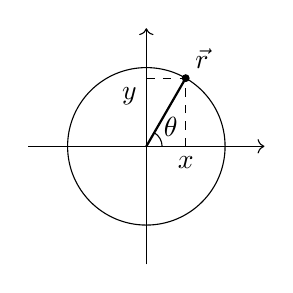
\begin{tikzpicture}[scale=1.0]
        % axis
        \draw[->] (-1.5,0) -- (1.5, 0);
        \draw[->] (0,-1.5) -- (0, 1.5);
        
        \draw (0,0) circle (1.0);
        \fill (0.5, 0.866) circle (0.05);
        \draw[dashed] (0.5, 0) -- (0.5, 0.866);
        \draw[dashed] (0, 0.866) -- (0.5, 0.866);
        \draw[thick] (0,0) -> (0.5, 0.866);
        \node[below] at (0.5, 0) {$x$};
        \node[below left] at (0.0, 0.866) {$y$};
        \node[above right] at (0.5, 0.866) {$\vec{r}$};
        \draw (0.2,0) arc (0:60:0.2);
        \node[above right] at (0.1,0) {$\theta$}; 
    
    \end{tikzpicture}
    \caption{环上的粒子}
\end{figure}
势函数
\begin{align}
    V(x,y) = \begin{cases}
        0, \quad & \sqrt{x^2 + y^2} = R,\\
        \infty, \quad &\sqrt{x^2 + y^2} \neq R, 
    \end{cases}
\end{align}
% 【讨论势能】
写出哈密顿量
\begin{align}
    \hat H = -\frac{\hbar^2}{2m} \left(\pdv[2]x + \pdv[2]y\right) + V(x,y)
\end{align}
此时无法分离变量 $\psi(x,y) \neq X(x) Y(y)$。如果将其变换到极坐标下,那么便可以分离变量,
\begin{align}
    \psi(r,\theta) = R(r) \Theta(\theta)
\end{align}
到底能否分离变量,求解完了才知道。

\chat{%
对波函数变换之后,还要把动能算符变换到极坐标下。这种变换相当于高中的难题,暴力求解比较麻烦,通常需要在求解开始时做非常巧妙的代换。尝试直接求解。}
首先,波函数的偏导不管在任何坐标下都是相等的,
\begin{align}
    \pdv[2]x \psi(x,y) = \pdv[2]{x} \psi(r,\theta),
\end{align}
用链式法则求解
\begin{align}
    &\pdv{\psi}{x} = \pdv{\psi}{r} \pdv{r}{x} + \pdv{\psi}{\theta} \pdv{\theta}{x},\\
    &\pdv{\psi}{y} = \pdv{\psi}{r} \pdv{r}{y} + \pdv{\psi}{\theta} \pdv{\theta}{y},
\end{align}
有几个显然的关系,
\begin{align}
    r^2 = x^2 + y^2, \quad \sin \theta = \frac xr,\quad \cos\theta = \frac yr,
\end{align}
径向对坐标的偏导,
\begin{align}
    \pdv{r}{x} = \pdv{x} \sqrt{x^2 + y^2} = \frac 12 \frac{2x}{\sqrt{x^2 + y^2}} = \frac xr = \cos\theta,
\end{align}
角度对坐标的偏导,利用 $\theta = \arccos \frac xr, x\in[0,\pi)$,
\begin{align}
    \pdv{\theta}{x} &= \pdv{x} \arccos \frac xr = -\frac1{\sqrt{1- \frac{x^2}{r^2}}} \left(\frac xr\right)^{\prime} \\
    &= -\frac ry \left(\frac 1r - \frac x{r^2} \frac xr\right) 
    = -\frac 1y \left(1 - \frac{x^2}{r^2}\right) \\
    &= -\frac{y}{r^2} = - \frac{\sin\theta} r, 
\end{align}
以上化简假设了 $\theta$ 在第一象限($x,y>0$),对于三四象限的角($y < 0$)需要加负号。
\begin{lstlisting}
(* 第一象限内的偏导 *)
D[ArcCos[x/Sqrt[x^2 + y^2]], x];
Simplify[%, Assumptions -> {x > 0, y > 0}]
>> -(y/(x^2 + y^2))
\end{lstlisting}

% 2022-10-17 08:54:22  Wenbin Fan @FDU
% 第二节课
% 下面得快一点了
那么对于波函数的导数
\begin{align}
    \pdv{\psi(x,y)}{x} = \cos\theta \pdv{\psi(r,\theta)}{r} - \frac{\sin\theta} r \pdv{\psi(r,\theta)}{\theta}, 
\end{align}
所以直接可给出
\begin{align}
    & \pdv{x} = \cos\theta \pdv{r} - \frac{\sin\theta}r \pdv{\theta},\\
    & \pdv{y} = \sin\theta \pdv{r} + \frac{\cos\theta}{r} \pdv{\theta},
\end{align}

再做二次偏导
\begin{align}
    \pdv[2]{\psi(x,y)}{x} = \pdv{x} \left(\cos\theta \frac{\psi}r - \frac{\sin\theta}r \pdv{\psi}{\theta}\right)
    \label{eq:polar_2nd_derv}
\end{align}
其中第一项
\begin{align}
    \pdv{x} \left(\cos\theta\pdv{\psi}{r}\right) 
    &= \pdv{\cos\theta}{x}\pdv{\psi}{r} + \cos\theta \pdv{x} \pdv{\psi}{r} \\
    &=\frac{\sin^2\theta}{r} \pdv{\psi}{r} + \cos\theta \left(\pdv[2]{\psi}{r} \pdv{r}{x} + \pdv[2]{\psi}{r}{\theta} \pdv{\theta}{x}\right) \\
    & = \frac{\sin^2\theta}{r} \pdv{\psi}{r} + \cos\theta \left( \cos\theta \pdv[2]{\psi}{r} - \frac{\sin\theta}{r} \pdv[2]{\psi}{r}{\theta}\right)
\end{align}
利用了
\begin{align}
    \pdv{x} \cos\theta = - \sin\theta \pdv{\theta}{x} = \frac{\sin^2\!\theta}{r},
\end{align}
第二项
\begin{align}
    \pdv{x} \left(\frac{\sin\theta}{r}\pdv{\psi}{x}\right) 
    &= - \frac{2\sin\theta \cos\theta}{r^2} \pdv{\psi}{\theta} + \frac{\sin\theta}r \left(\pdv[2]{\psi}{r}{\theta} \pdv{r}{x} + \pdv[2]{\psi}{\theta} \pdv{\theta}{x}\right)\\
    &=- \frac{2\sin\theta\cos\theta}{r^2} \pdv{\psi}{\theta} + \frac{\sin\theta \cos\theta}{r} \pdv[2]{\psi}{r}{\theta} - \frac{\sin^2\theta}{r^2} \pdv[2]{\psi}{\theta},
\end{align}
利用了
\begin{align}
    \pdv{x} \frac{\sin\theta}{r} = \pdv{x} \frac{y}{r^2} = \frac{-2y}{r^3} \pdv{r}{x} = -\frac{2\sin\theta\cos\theta}{r^2},
\end{align}
\begin{lstlisting}
(* 对 x 的二阶偏导,输出略 *)
D[\[Psi][Sqrt[x^2 + y^2], ArcCos[x/Sqrt[x^2 + y^2]]], {x, 2}];
Simplify[%, 
   Assumptions -> {x > 0, y > 0}] /. {y -> Sqrt[
    r^2 - r^2 Cos[\[Theta]]^2], x -> r Cos[\[Theta]]};
Simplify[%, Assumptions -> {r > 0, \[Theta] > 0, \[Theta] < Pi/2}]
\end{lstlisting}
于是
\begin{align}
    \pdv[2]{\psi(x,y)}{x}     
    &= \pdv{x} 
    \left(\cos\theta \pdv{\psi}{r} - \frac{\sin\theta}{r} \pdv{\psi}{\theta}\right) \\
    &= \cos^2\theta \pdv[2]{\psi}{r} - \frac{2\sin\theta\cos\theta}{r} \pdv[2]{\psi}{r}{\theta} + \frac{\sin^2\theta}{r^2} \pdv[2]{\psi}{\theta} \notag \\
    &\phantom{=} \quad + \frac{\sin^2\theta}{r} \pdv[2]{\psi}{r} + \frac{2\sin\theta\cos\theta}{r^2} \pdv{\psi}{\theta},
\end{align}
同理
\begin{align}
    \pdv[2]{\psi(x,y)}{y} &= \sin^2\!\theta \pdv[2]{\psi}{r} + \frac{2\sin\theta \cos\theta}{r} \pdv[2]{\psi}{r}{\theta} + \frac{\cos^2\theta}{r^2} \pdv[2]{\psi}{\theta} \notag\\
    &\phantom{=}\quad+ \frac{\cos^2\theta}{r} \pdv{\psi}{r} - \frac{2\sin\theta \cos\theta}{r^2} \pdv{\psi}{\theta}, 
\end{align}
于是 \eqref{eq:polar_2nd_derv} 为
\begin{align}
    \pdv[2]{\psi}{x} + \pdv[2]{\psi}{y} &= \pdv[2]{\psi}{r} + \frac1{r^2} \pdv[2]{\psi}{\theta} + \frac1r \pdv{\psi}{r} \\
    &=\pdv[2]{\psi}{r} + \frac1r \pdv{\psi}{r} + \frac1{r^2}\pdv[2]{\psi}{\theta}, 
\end{align}

最终哈密顿量写为
\begin{align}
    \hat H = - \frac{\hbar^2}{2m} \left(\pdv[2]{x} + \pdv[2]{y}\right) = -\frac{\hbar^2}{2m} \left(\pdv[2]{\psi}{r} + \frac1r \pdv{\psi}{r} + \frac1{r^2}\pdv[2]{\psi}{\theta}\right),
\end{align}
考虑本例中势能的特殊性,其径向部分为常数 $R$,因此哈密顿量仅与 $\theta$ 有关,
\begin{align}
    \hat H = - \frac{\hbar^2}{2mR^2} \pdv[2]{\theta} = -\frac{\hbar^2}{2I} \pdv[2]{\theta},
\end{align}
其中
\begin{eqnarray}
    I = m R^2
\end{eqnarray}
称之为\boldtext{转动惯量} momentum of inertia。%注意到 $\omega = \theta / t$,

薛定谔方程为
\begin{align}
    \hat H \varphi(\theta) &= E\varphi(\theta)\\
    - \frac{\hbar^2}{2I} \pdv[2]{\varphi}{\theta} &= E\varphi
\end{align}
整理得到
\begin{align}
    \pdv[2]{\varphi(\theta)}{\theta} + M^2 \varphi(\theta) = 0, \quad M^2 = \frac{2IE}{\hbar^2},
\end{align}
这是个二阶微分方程,设 $\varphi(\theta) = \ee^{s\theta}$,有
\begin{align}
    s^2 \ee^{s\theta} + M^2 \ee^{s\theta} = 0
\end{align}
得到
\begin{align}
    s^2 = - M^2 \Rightarrow s = \pm \ii M,
\end{align}
可得方程通解
\begin{align}
    \varphi(\theta) = A \ee^{\ii M\theta} + B \ee^{-\ii M \theta}
\end{align}
共有三个待求变量 $\{A, B, M\}$。

给出通解之后,利用边界条件得到量子化结果。在解无限深势阱的时候,利用了波函数连续、导数连续的条件。我们这里的二位极坐标体系,边界就是粒子转过 $2\pi$ 后又回来,所以有周期性边条件,
\begin{align}
    \varphi(\theta) = \varphi(\theta + 2\pi),
\end{align}
解得
\begin{align}
    \ee^{\ii M\, 2\pi} = 1 \Rightarrow M = 0, \pm 1, \pm 2, \cdots,
\end{align}
这里的 $M$ 称之为磁量子数 magnetic quantum number,从而可以解出能量
\begin{align}
    M^2 = \frac{2IE}{\hbar^2} \Rightarrow E = \frac{M^2\hbar^2} {2I} = \frac{M^2h^2} {8\pi^2 L},
\end{align}
知道了分子的转动惯量,就可以求出转动的精确谱、能量间隔。


讲到了转动,就必须要讲到角动量。角动量算符在经典力学中的定义为
\begin{align}
    \bm L = \bm r \times \bm p = \bm r \times m\bm v, 
\end{align}
对应的是右手定则。
分量形式
\begin{align}
    &L_x = y p_z - zp_y, \\
    &L_y = z p_x - x p_z, \\
    &L_z = x p_y - y p_x, 
\end{align}
微观体系中角动量是什么样的?

角动量的量子化 quantization,
\begin{align}
    \hat L_z = x \hat p_y - y \hat p_x = - \ii \hbar \left(x \pdv{y} - y \pdv{x}\right),
\end{align}
可以通过极坐标的变化求解出极坐标下的表达式,
\begin{align}
    \hat L_z = -\ii \hbar \pdv{\theta},
\end{align}
作为作业。
\homework{\textbf{5.2}  推导极坐标下的 $z$ 轴角动量算符 $\hat L_z$ 表达式。}
\chat{%
有个问题,我们说是量子化,其实直接用了动量算符的定义,但这是演绎,不是推导。如果在经典情况,$x$ 的位置无所谓,放在算符前后均可,以便跟量子情况相对于,实际上量子化不是直接加个 $\hat\cdot$ 得到的,角动量的量子化过程不具有普适性。
}

已经求出了环上粒子的通解,将
角动量算符作用到通解波函数上,
\begin{align}
    \hat L_z \varphi(\theta) \overset{?}{=} C\varphi(\theta),
\end{align}
会得到常数 $C$ 吗?
\chat{%
不一定对吧,作用上去之后会有两个相反的系数 $\ii m$。这就很像动量算符和动能算符的关系,我们知道动量算符、动能算符是互易的,原则上可以共享同一个本征函数。
% \homework{\textbf{5.2} (\emph{continued}) 证明}

环上粒子的哈密顿量 $\hat H$ 和角动量 $\hat L_z$ 显然是对易的,所以它们可以共享相同的本征函数。通过构造本征函数,能求出通解,因为 $m$ 是任意的。并不要求角动量的本征函数是 $z$ 方向的。

量子力学基本假设第四条告诉我们,线性厄米算符给出来的本征函数是完备集,意思是任何函数都可以用这个完备集展开。二者共享本征函数的意思是,那么用这个共享的本征函数可以描述任何状态,无需只用一个或另一个,那么通解中的 $A$ 和 $B$ 可以去掉其中一个。剩下的一个代表它既是哈密顿量的本征函数,也是 $\hat L_z$ 的本征函数。

我们在实际的体系中,为什么要做这个事儿?正常来说,我们解薛定谔方程,通常只要基态能量,并不关心波函数是否是 $\hat L_z$ 的本征函数。在真实观测中,观测到的不仅是基态,还有各种的激发态。比如磁场下的分子,光谱中能看到各种磁量子数导致的细分。
% 【一大段讲述】
% 实际体系光谱,还有磁量子数。
% 状态波函数不仅是【】还是【】的本征函数,所以这个态是为了解磁量子数时光谱的细分【】。

在解氢原子体系时,能量只与 $n$ 有关。通过连带勒让德方程,还有 $m_l$ 等量子数。哈密顿算符是不区分 2p$_{-1}$、2p$_1$ 等,从实验中是可以同时准确观测到分量的。为什么能准确测量能量,同时在光谱中看到精确的磁量子数?因为哈密顿算符 $\hat H$ 和角动量 $\hat L$ 是对易的。动能和位置算符是不对易的,所以无法同时准确测量。
}

% 2022-10-17 13:24:54  Wenbin Fan @FDU
% 下午
\courseTime{下午}
简单回顾下早上的内容。
\chat{%
想要了解任何感兴趣的体系,都要解薛定谔方程。目前的波函数都是不含时的,即定态方程。今天求解的势能函数是二维的,这是与之前最大的不同。通常二维势能难以在 Cartesian 空间求解,由合适的坐标变换可以简化求解过程。最契合环势能的坐标是极坐标,因此很自然地分离变量。

将环形势能变换到极坐标下,此时哈密顿量仅与 $\theta$ 有关,引入周期性边条件,得到磁量子数。随后演绎了角动量 $\hat l_z$ 的算符表示。

环运动的通解是两个本征函数的线性组合,包含了顺时针和逆时针旋转的组合。哈密顿算符和 $\hat l_z$ 是队医的,可以构造同时属于二者的本征函数完备集,所以可以把 $\varphi(\theta)$ 写成 $A \ee^{\ii m \varphi}$ 的形式。
}

接上午的求解。由归一化确定 $A$,
\begin{align}
    \int_0^{2\pi} \varphi^*(\theta) \varphi(\theta) \dd\theta = A^2 \int_{0}^{2\pi} \dd\theta = 2\pi A^2 = 1,
\end{align}
解之得
\begin{align}
    \varphi(\theta) = \frac{1}{\sqrt{2\pi}} \ee^{\ii m \theta}, \quad \rho(\theta) = |\varphi(\theta)|^2 = \frac1{2\pi},
\end{align}
因此波函数没有节点,任何地方的取值都是一样。

\chat{%
我们现在求解的模型,都是希望贴近化学真实体系,与这个模型最相近的是苯环。}

\homework{\textbf{5.2}  对于一维环形势箱,其能级为 
\begin{align}
    E_n = \frac{n^2 h^2}{8\pi^2 m R^2}, \quad n = 0, 1, 2, \cdots,
\end{align}
苯环的 $\pi$ 电子可近似看成是电子限制在一个环上的运动,$\pi$ 电子的半径是 \SI{1.4}{\angstrom},请以一维环形势箱的模型计算其最低激发能。

(以下选做)激发能的实验值是 \SI{2600}{\angstrom},讨论误差可能的来源。
}
\chat{%
随意讨论,真实的苯和离域电子的区别是什么。下周习题课,再下次求解熟悉的氢原子,我们现在从二维拓展到三维,为求解氢原子做准备。
}

\section{柱面上的粒子}
\textbf{先讲一个简单的三维体系,(同学:球)真会找,找了个最难的。}

最简单的是自由粒子,三维自由粒子的算符,
\begin{align}
    \hat H = -\frac{\hbar^2}{2m} \left(\pdv[2]{x} + \pdv[2]{y} + \pdv[2]{z}\right), \quad \hat H \psi(x,y,z) = E \psi (x,y,z),
\end{align}
通过分离变量,可以解耦,求出来各个分量的波函数。

\textbf{
其次是无限深势阱的拓展,三维势能箱。比球简单一些的(安静),是圆柱啊!圆柱可以分离变量。接近真实的碳纳米管,这里以铜丝为例。}
\homework{\textbf{5.3}  一圆柱体,长为 $l$、半径为 $R$,求解该圆柱体体系的能级,这里的势函数定义为
\begin{align}
    V(x,y,z) = \begin{cases}
        0, \quad &(x,y,z) \in \Omega,\\
        +\infty, \quad &(x,y,z) \notin \Omega,
    \end{cases}
\end{align}
其中
\begin{align}
    \Omega = \left\{(x,y,z) \, |\,  x^2+y^2 \leqslant R^2, 0\leqslant z\leqslant l\right\}. 
\end{align}
可参考徐昕老师 2000 年的文章 Jian-Lin Yao, Xin Xu, De-Yin Wu, et al, \emph{Chem. Commum.} 2000, 1627。
}
\chat{%
这些东西已经超越了课堂内容,但也确实是关于课堂内容触手可及的拓展。如果你会算这些习题,其实你已经可以做一些科研工作了。

现在计算机发达,很多人已经习惯了用 Gaussian 软件,用各种基函数展开波函数。
% 【】有助于掌握背后的物理。
化学从简单模型演变到复杂,越来越难算,主要源自于实验的精度越来越高。早期的实验,可控性很差,无法控制合成多孔材料、超分子等,无法控制形貌,只能通过宏观的温度等辅助合成。当近代实验操控能力增强,比如精准化学可以 100\% 操控反应物和产物,人们能制造出更精确的催化剂。这时计算化学便可以辅助实验,得到活性最高的形貌。
% 精确操控形状,什么形状有用?
% 【】【】【】【】【】

再复杂一点的,是球面上运动的粒子。
}

\section{球面上运动的粒子}
哈密顿量写出来
\begin{align}
    \hat H = -\frac{\hbar^2}{2m} \left(\pdv[2]x + \pdv[2]y + \pdv[2]z\right) + V(x,y,z),
\end{align}
其中势能
\begin{align}
    V(x,y,z) = \begin{cases}
        0, \quad &\sqrt{x^2+y^2+z^2} = r = R, \\
        \infty, \quad &\text{其它},
    \end{cases}
\end{align}
画出势能,坐标轴的定义是右手定则(四指从 $x$ 转向 $y$,大拇指指向 $z$),注意这里的 $\theta$ 是 $\bm r$ 与 $z$ 轴的夹角。
\begin{figure}
    \centering
    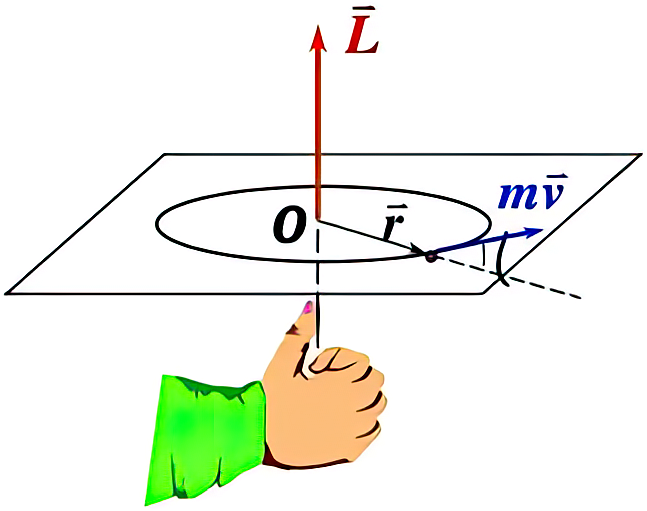
\includegraphics[width=3cm]{fig/angular_momentum.png}
    \caption{角动量方向}
    \label{fig:ang_direction}
\end{figure}

定义好坐标轴后,写出坐标映射
\begin{align}
    & x= r\,\sin\theta \, \cos\varphi, \\
    & y = r\,\sin\theta \, \sin\varphi, \\
    & z = r\,\cos\theta,
\end{align}
体积元变化
\begin{align}
    \Delta V = \Delta x \,\Delta y\, \Delta z,
\end{align}
\begin{figure}[tbp]
    \centering
    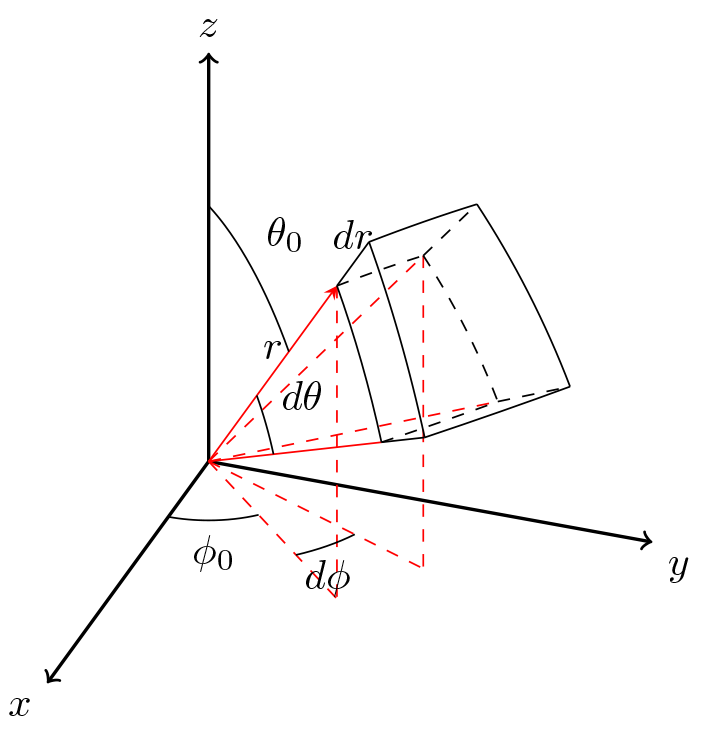
\includegraphics[width=4cm]{fig/3d_int_element.png}
    \caption{求坐标中的积分微元}
    % ref: https://blog.csdn.net/TanWaiwai_yy/article/details/104710427
\end{figure}
根据推导,有
\begin{align}
    \Delta V & =\dd s \, \dd r \\
    & = r \, \dd\theta \, r\sin\theta \, \dd\varphi \dd r \\
    & = r^2 \sin\theta \dd\theta \dd\varphi \dd r,
\end{align}
暴力推导的话,今天就别下课了。这里利用高级的数学方法,即利用 Jacob 矩阵来变换坐标系,
\begin{align}
    J = 
    \begin{pmatrix}
    \pdv{x}{r} & \pdv{x}{\theta} & \pdv{x}{\varphi} \\
    \pdv{y}{r} & \pdv{y}{\theta} & \pdv{y}{\varphi} \\
    \pdv{z}{r} & \pdv{z}{\theta} & \pdv{z}{\varphi}
    \end{pmatrix}, \quad 
    \begin{pmatrix}
        \pdv{r} \\ \pdv{\theta} \\ \pdv{\varphi}
    \end{pmatrix}
    = J 
    \begin{pmatrix}
        \pdv{x} \\ \pdv{y} \\ \pdv{z}
    \end{pmatrix},
\end{align}
直接得到结果,动能算符在极坐标下的表述,
\begin{align}
    \hat T = - \frac{\hbar^2}{2m} \left(
        \pdv[2]r + \frac2r \pdv{r} + \frac1{r^2} \hat \Lambda^2
    \right),
\end{align}
其中
\begin{align}
    \hat \Lambda^2 &= \frac1{\sin^2\theta} \pdv[2]{\varphi} + \frac1{\sin\theta} \pdv{\theta} \left(\sin\theta \pdv{\theta}\right) \\
    & = \frac1{\sin^2\theta} \pdv[2]{\varphi} + \cot\theta \pdv{\theta} + \pdv[2]{\theta},
\end{align}
这个算符 $\hat \Lambda$ 包含了动能中所有角度部分的能量,即角动量相关的能量,它一定与角动量相关。接下来很自然地考虑,三维的角动量如何考虑?

我们已经给出了二维的角动量,角动量的方向向外,沿着第三个坐标轴 $z$。角动量算符
\begin{align}
    \bm L = \bm r \times \bm p = \bm r \times m \bm v,
\end{align}
三个分量为
\begin{align}
    &\hat L_x = -\ii\hbar \left(y \pdv{z} - z \pdv{y}\right), \\
    &\hat L_y = -\ii\hbar \left(z \pdv{y} - y \pdv{z}\right), \\
    &\hat L_z = -\ii\hbar \left(x \pdv{y} - y \pdv{x}\right),
\end{align}
% 【还有两个式子没列上】
回顾两个例子中的解,
\begin{alignat}{2}
    &\text{二维极坐标} \quad &&\hat L_z = -\ii\hbar \pdv{\theta}, \\
    &\text{三维极坐标} \quad && \hat L_z = -\ii\hbar \pdv{\varphi},
\end{alignat}
% 【这里角动量分量好像不太对耶】
\homework{\textbf{5.4} 证明 
\begin{align}
    \hat L_x = -\ii\hbar \left(
        \sin\varphi \pdv{\theta} + \cot\theta \cos\varphi \pdv{\varphi}
    \right), \\
    \hat L_y = -\ii\hbar \left(
        \cos\varphi \pdv{\theta} - \cot\theta \sin\varphi \pdv{\varphi}
    \right),
\end{align}
并且利用
\begin{align}
    \hat L = \hat L_x \bm i + \hat L_y \bm j + \hat L_z \bm k
\end{align}
推导
\begin{align}
    \hat L^2 &= \hat L_x^2 + \hat L_y^2 + \hat L_z^2 \\&= -\hbar^2 \left(
        \frac1{\sin^2\theta} \pdv[2]{\varphi} + \cot\theta \pdv{\theta} + \pdv[2]{\theta}
    \right) \\
    &= -\hbar^2 \Lambda^2,
\end{align}
}

% 【推导 theta varphi 相关的式子】
% 【必须求解耦合的方程了】
% 当前体系的哈密顿量,
% \begin{align}
%     \hat H = -\frac{\hbar^2}{2mR^2} \hat\Lambda^2 = \frac1{2mR^2} \hat L^2 = - \frac1{2I},
% \end{align}
薛定谔方程
\begin{align}
    -\frac{\hbar^2}{2mR^2} \hat \Lambda^2 Y(\theta,\varphi) = E Y(\theta, \varphi), 
\end{align}
% 2022-10-17 14:24:07  Wenbin Fan @FDU
% 最后一节啦!
径向部分的偏导全部为 0,那么能否分离变量?
\begin{align}
    Y(\theta,\varphi) \overset{?}{=} \Theta(\theta) \Phi(\varphi),
\end{align}
尝试分离后代回,
\begin{align}
    \hat \Lambda^2  \Theta(\theta) \Phi(\varphi) + M^2  \Theta(\theta) \Phi(\varphi) = 0,
\end{align}
把 $\hat \Lambda^2$ 的定义代入,
\begin{align}
    \left(\frac1{\sin^2\theta} \pdv[2]{\varphi} + \cot\theta \pdv{\theta} + \pdv[2]{\theta}\right) \Theta(\theta) \Phi(\varphi) + M^2  \Theta(\theta) \Phi(\varphi) = 0, \notag\\
    \frac{\Theta(\theta)}{\sin^2\theta} \pdv[2]{\varphi} \Psi(\varphi) + \cot\theta \Psi(\varphi) \pdv{\theta} \Theta(\theta) + \Psi(\varphi) \pdv[2]{\theta} \Theta(\theta) + M^2 \Theta(\theta) \Psi(\varphi) = 0,
\end{align}
两边同时除以 $\Theta(\theta) \Phi(\varphi)$,
\begin{align}
    \frac{1}{\sin^2\theta \Psi(\varphi)} \pdv[2]{\varphi} \Psi(\varphi) + \frac{\cot\theta}{\Theta(\theta)} \pdv{\theta} \Theta(\theta) + \frac1{\Theta(\theta)} \pdv[2]{\theta} \Theta(\theta) + M^2 &= 0 \notag\\
    \underbrace{\frac{1}{\Psi(\varphi)} \pdv[2]{\varphi} \Psi(\varphi)}_{\varphi} 
    + 
    \underbrace{\frac{\sin\theta\,\cos\theta}{\Theta(\theta)} \pdv{\theta} \Theta(\theta) + \frac {\sin^2\theta}{\Theta(\theta)} \pdv[2]{\theta} \Theta(\theta) + M^2 \sin^2\theta}_{\theta}
    &= 0,
\end{align}
第一项只跟 $\varphi$ 有关,后面三项只跟 $\theta$ 有关,所以可以分开,分别移动到等号两端
\begin{align}
    \frac{1}{\Psi(\varphi)} \pdv[2]{\varphi} \Psi(\varphi) = - \left[
        \frac{\sin\theta\,\cos\theta}{\Theta(\theta)} \pdv{\theta} \Theta(\theta) + \frac {\sin^2\theta}{\Theta(\theta)} \pdv[2]{\theta} \Theta(\theta) + M^2 \sin^2\theta
    \right]
    \label{eq:sphere_surface_sep_done}
\end{align}
令左侧等于常数 $N$
\begin{align}
    \frac{1}{\Psi(\varphi)} \pdv[2]{\varphi} \Psi(\varphi) = N \Rightarrow  \pdv[2]{\varphi} \Psi(\varphi) = N \Psi(\varphi), 
\end{align}
取 $\Psi(\varphi) = \ee^{s\varphi}$,当 $N>0$ 时,$s = \pm\sqrt N$,$\Psi(\varphi) = \ee^{\pm \sqrt N \varphi}$ 发散、非品优,舍弃。%【】【】【N<0】
当 $N<0$ 时,$s = \pm\ii\sqrt{-N}$,$\Psi(\varphi) = \ee^{\pm\ii\sqrt N}$。

设 $N = - m_l^2$,得到
\begin{align}
    \Psi(\varphi) = A \ee^{\ii m_l \varphi} + B \ee^{-\ii m_l \varphi},
\end{align}

% 【共同本征函数】
因为
$\hat L^2$ 与 $\hat L_z$ 的共同本征函数解,
\begin{align}
    \Psi(\varphi) = A \ee^{\ii m_l \varphi} = \frac1{\sqrt{2\pi}} \ee^{\ii m_l \varphi}, \quad m_l = 0, \pm1, \pm2, \cdots,
\end{align}
因为有共同的本征值,那么 \eqref{eq:sphere_surface_sep_done} 右侧 $\Theta$ 相关的项等于 $-m_l^2$,
\begin{align}
    - \left[
        \frac{\sin\theta\,\cos\theta}{\Theta(\theta)} \pdv{\theta} \Theta(\theta) + \frac {\sin^2\theta}{\Theta(\theta)} \pdv[2]{\theta} \Theta(\theta) + M^2 \sin^2\theta
    \right] = -m_l^2,
\end{align}
整理得
\begin{align}
    \sin\theta\cos\theta \pdv{\theta} \Theta(\theta) + \sin^2\theta \Theta(\theta) = (m_l^2 - M^2 \sin^2\theta) \Theta(\theta),
\end{align}
在以前求解的体系中,能量是完全量子化的,但是这里的 $\theta,\varphi$ 完全不是,因为二者的量子数相互有关系,关于 $\varphi$ 的量子数要代入到 $\theta$ 的求解中。

该方程的解称作\boldtext{连带勒让德多项式}。目前还是太复杂了些,做一些变量代换。首先三角函数看起来就很麻烦,替换掉,设 $x = \cos\theta$,则 $\Theta(\theta) = y(x)$,求这个代换的偏导数,
\begin{align}
    &\pdv{\theta}\Theta(\theta) = \pdv{y(x)}{x} \pdv{x}{\theta} = \pdv{y(x)}{x}(-\sin\theta),\\
    &\pdv[2]{\theta} \Theta(\theta ) = 
    -\cos \pdv{y(x)}{x} - \sin\theta \pdv[2]{y(x)}{x} \pdv{x}{\theta} \\
    &\phantom{\pdv[2]{\theta} \Theta(\theta )} = 
    -\cos \pdv{y(x)}{x} + \sin^2\theta \pdv[2]{y(x)}{x}, 
\end{align}
代换完了是
\begin{multline}
    - x(1-x^2) \pdv[2]{y(x)}{x} + (1-x^2) \left[
        -x \pdv{y(x)}{x} + (1-x^2) \pdv[2]{y(x)}{x}
    \right] \\= \left[m_l^2 - M^2(1-x^2)\right] y(x),
\end{multline}
观察到其中每一项都含有 $(1-x^2)$,两边同时除以它。按照导数的次数排列,有
\begin{align}
    (1-x^2) y''(x) - 2x\, y'(x) + \left(M^2 - \frac{ml^2}{1-x^2}\right) y(x) = 0.
    \label{eq:legendre_ordered} % 按导数次序排列的
\end{align}

现在还不能求解它,因为当 $x = \cos\theta = \pm1$ 时有奇点,必须先消除奇点。

\textbf{(1) 消除奇点},当 $x = \pm 1$ 时,
\begin{align}
    y(x) = (1 - x^2)^n H(x),
\end{align}
书上会告诉你当 $n = \frac{|m_l|}2$ 时可以消除,那么为什么呢?我们从头开始推导这个结果,即直接把 $n$ 代回原式。求出偏导方便一些,
\begin{align}
    &\pdv{y(x)}{x} = -2n x (1-x^n)^{n-1} H_n(x) + (1-x^2)^n H'(x),
\end{align}
二阶偏导稍麻烦
\begin{align}
    \pdv[2]{y(x)}{x} &= -2n x \left[
        (1-x^2)^{n-1} - 2(n-1)x^2(1-x^2)^{n-2}
    \right]H(x)  \notag\\
    &\quad\quad
    - 2n x(1-x^2)^{n-1} H'(x) 
    - 2n x(1-x^2)^{n-1} H'(x) \notag\\
    &\quad\quad + (1-x^2)^n H''(x) \\
    & = \left[
        -2n (1-x^2)^{n-1} + 4n (n-1) x^2 (1-x^2)^{n-2}
    \right] H(x) \notag\\
    &\quad\quad - 4nx(1-x^2)^{n-1} H'(x) + 
    (1-x^2)^n H''(x)
\end{align}
这时候再代回原式 \eqref{eq:legendre_ordered}
\begin{multline}
    \left[
        -2n (1-x^2)^n + 4n(n-1) x^2 (1-x^2)^{n-1}
    \right] H(x) \\
    - 4nx(1-x^2)^n H'(x) + (1-x^2)^{n+1} H''(x) \\
    + 4nx^2 (1-x^2)^{n-1} H(x) 
    - 2x (1-x^2)^n H'(x) \\
    +\left[
        M^2 (1-x^2)^n - m_l^2 (1-x^2)^{n-1}
    \right] H(x) = 0,
\end{multline}
合并同类项,
\begin{multline}
    (1-x^2)^{n+1} H''(x) - 2x(2n+1) (1-x^2)^n H'(x) 
    \\+ 
    \left[
        -2n (1-x^2)^n + 4n^2 x^2 (1-x^2)^{n-1} - m_l^2 (1-x^2)^{n-1} + M^2 (1-x^2)^n
    \right] H(x) \\= 0
\end{multline}
再化简,
\begin{align}
    (1-x^2) H''(x) - 2x(2n+1) H'(x) + \left[
        -2n + \frac{4n^2x^2 - m_l^2}{1-x^2} + M^2
    \right] H(x) = 0
\end{align}
也就是当 $4n^2 = m_l^2$ 时,有
\begin{align}
    \frac{m_l^2 (x^2 - 1)}{1 - x^2} = - m_l^2,
\end{align}
令 $n = \frac{|m_l|}2$,即
\begin{align}
    y(x) = (1 - x^2)^{|m_l|/2} H(x),
\end{align}
有
\begin{align}
    (1-x^2) H''(x) - 2\left(|m_l| + 1\right)x \, H'(x) + \left(m^2 - m_l^2 - |m_l|\right) H(x) = 0. 
\end{align}

\chat{%
整个解法从头到尾写下来很累的,但是每一步都有逻辑。量子的教科书上都是这个结论,读者难以知道整个过程。

在学习特殊函数或者数学物理方程时,最有创造性的一点是一开始选什么样的初猜,即选择什么样的通解。球面上的粒子也是一样,从尝试分离变量开始,再到消奇点,很幸运有连带勒让德函数这个解。

% 2022-10-17 15:08:33  Wenbin Fan @FDU
% 快下课了 XD
% 这段求解过程好乏味……
下节课继续讲幂级数求解法。
}













\section{复习}
\courseTime{Oct 24}
% 2022-10-24 07:59:36  Wenbin Fan @FDU
\chat{%
是人变少了吗,还是坐后面去了(笑)。

我们今天有节习题课,下周讲氢原子,慢慢接近于真实体系了,后面会安排上机,把我们的超算给同学们用。

今天要把上次课讲完,同时补充一些前面的内容。下午两节课习题课,助教来上。
}

上周课我们讲了转动角动量。

\chat{%
二维体系的时候,粒子在环形圆上运动,相当于势函数的边界条件跟 $r$ 能更好地分离变量,所以要做坐标变换,最关键的是动能部分的坐标变换。通过变换动能,得到了分离变量的哈密顿量。势函数是 delta 函数,因此哈密顿量跟自由粒子是一样的。

哈密顿量变换后,因为径向不变,其中对径向的偏导为 0,所以哈密顿量之跟角度有关。转动惯量定义为 $I = mr^2$。由周期性边界条件,得到了磁量子数。

随后定义了角动量,特别是 $z$ 轴的角动量。
由于 $l_z$ 对易,可以构造共同的本征函数完备集,
方向性可以体现在 $m$ 的正负上。一维拓展到三维。

对于球面上的粒子,与圆环上的粒子类似,势能只与 $r$ 有关,一样要做坐标变换。动能算符,其中的转动部分含有角度分量。二维中,$xOy$ 平面的角度是 $\theta$,三维中,角动量与 $z$ 轴的夹角是 $\theta$。

% $\hat L^2$ 的
第一次涉及到两个变量耦合的求解,成功地分离变量。

我们对勒让德方程做变换,是为了利用数学物理方程中的结论,更方便地求解。勒让德方程已经被研究得非常透彻。我们不是数学系、物理系,但鼓励学习数学物理方程、泛函分析等。
比如,导出薛定谔方程,需要有强大的数学直觉,我们现在学习也是为了以后寻找物理规律。
}

上节课讲到了\boldtext{幂级数展开},继续讲。勒让德方程里有一阶、二阶偏导,
\begin{align}
    H(x) = \sum_{j=0}^{\infty} a_j x^j, \quad H'(x) = \sum_{j=1}^{\infty} j a_j x^{j-1}, \quad H''(x) = \sum_{j=2}^{\infty} j(j-1) a_j x^{j-2},
\end{align}
得到了等间隔的递推公式
\begin{align}
    \sum_{j=1}^\infty
    \left\{
        (j+2)(j+1) a_{j+2} + \left[
            (j+ |m_l|)(j+ |m_l| +1) - M^2
        \right]a_j
    \right\} x^j = 0,
    % 2022-10-24 08:20:05  Wenbin Fan @FDU
\end{align}
若 $H(x)$ 是无穷级数,则 $H(x)$ 不是品优波函数。
所以,如果 $a_j$ 在 $k$ 截断,意味着这一项为 0,
\begin{align}
    a_{j+2} = \frac{(j+|m_l|)(j+|m_l|+1) - M^2}{(j+2)(j+1)} a_j,
\end{align}
参考 H. Eyring, J. Walter, Quantum Chemistry, \S 4. 

这里省略一些通用的推导。若 $H(x)$ 是无穷级数,则 $H(x)$ 不是品优波函数,当 $a_j$ 在 $k$ 截断,
\begin{align}
    (k+|m_l|)(k+|m_l|+1) - M^2 = 0, 
\end{align}
令 $l \equiv k + |m_l|$,则
\begin{align}
    M^2 = l(l+1),
\end{align}
其中
\begin{align}
    |m_l| = 0,1,2,\cdots, \quad l = 0,1,2,\cdots,
\end{align}
显然可知 $|m_l|_{\mathrm{max}} = l$。

% 2022-10-24 08:24:28  Wenbin Fan @FDU
再回到能量的量子化,体系的能量
\begin{align}
    - \frac{\hbar^2}{2m R^2} \hat\Lambda^2 Y(\theta, \varphi) = E Y(\theta, \varphi), 
    \label{eq:LambdaYEY}
\end{align}
分离变量得到
\begin{align}
    \hat \Lambda^2 \Theta(\theta) \Phi(\varphi) + M^2 \Theta(\theta) \Phi(\varphi)  = 0,
\end{align}
其中
\begin{align}
    M = E \frac{2mR^2}{\hbar^2} = \frac{2IE}{\hbar^2},
\end{align}
得到了能量的量子化
\begin{align}
    E = \frac{\hbar^2}{2I} \, l (l+1), \quad l = 0,1,2,\cdots,
\end{align}
与此同时,如果找到二者共同的本征函数,一定会有本征角量子数,并且角量子数 $m_l = 0, \pm1, \pm2, \cdots, \pm l$。

因为哈密顿算符 $\hat H$ 和 $l_z$ 是对易的。如果取二者共同的本征函数,
两个算符作用上去,
就会有两个量子数 $m_l$ 和 $l$,这也就是为什么把 \eqref{eq:LambdaYEY} 写成
\begin{align}
    - \frac{\hbar^2}{2I} \hat\Lambda^2 Y_{l,m_l}(\theta, \varphi) = \frac{\hbar^2}{2I} l(l+1) Y_{l,m_l}(\theta, \varphi). 
\end{align}
我们知道 $\hat \Lambda$ 和 $\hat L$ 是等价的,$\hat L^2 = -\hbar^2\hat L^2$,那么代入这个等式,有
\begin{align}
    \frac{1}{2I} \hat L^2 Y_{l,m_l}(\theta, \varphi) &= \frac{\hbar^2}{2I} l(l+1) Y_{l,m_l}(\theta, \varphi) \\
    \hat L^2 Y_{l,m_l}(\theta, \varphi) &= \hbar l (l+1) Y_{l,m_l}(\theta, \varphi)\label{eq:6_l_squared}
\end{align}
很自然地给出了角动量算符在三维体系中的本征函数。

后面求氢原子体系,当然要做一些额外的坐标变换,其势能函数只与径向有关(库伦算符),角度部分是球谐形式,所以我们求解的也是氢原子的角度部分。

\eqref{eq:6_l_squared} 中也能推导出 $z$ 方向的本征值,
\begin{align}
    \hat L_z = -\ii\hbar \pdv{\varphi} \Rightarrow \hat l_z Y_{l,m_l}(\theta, \varphi) = m_l Y_{l,m_l}(\theta, \varphi), 
\end{align}
\begin{align}
    |m_l|_{\mathrm{max}} = l, \quad \langle \hat l_z \rangle^2 |_{\mathrm{max}} = l^2, 
    \quad \langle \hat L^2 \rangle = l(l+1),
\end{align}
$z$ 方向一定有不确定性,类似于零点能。
% 【】一定会留下一份。
% 讲错了
% 2022-10-24 08:35:49  Wenbin Fan @FDU
也可以理解成「测不准原理」。
\begin{figure}
    \centering
    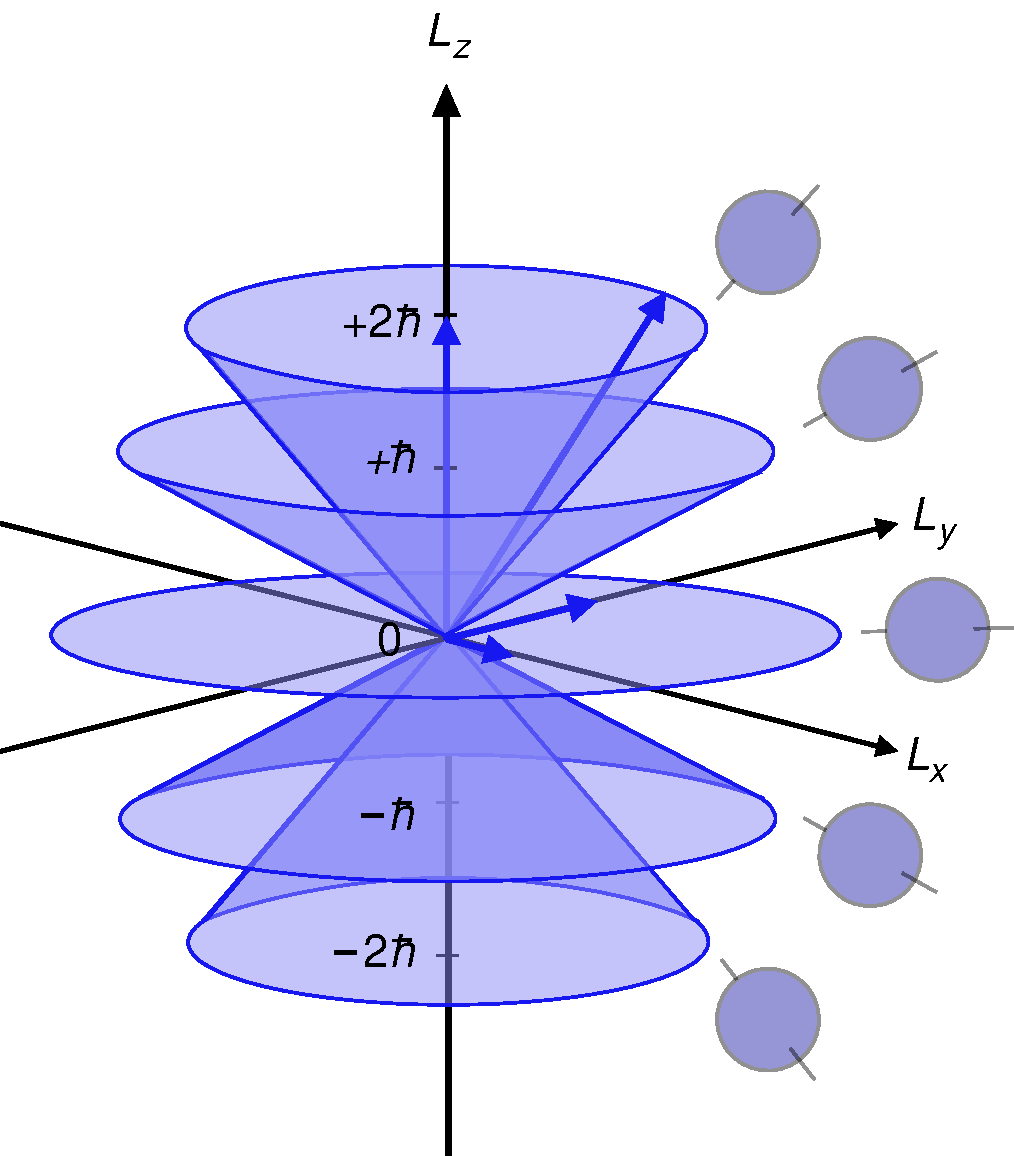
\includegraphics[height=3cm]{fig/angular_momentum_Wikipedia.pdf}
    \caption{角动量量子化}
\end{figure}

\homework{
    \textbf{6.1}  对于一个电子 $m_{\mathrm e} = \SI{9.11E-31}{\kilo\gram}$,以及一个陀螺 $m = \SI{0.02}{\kilo\gram}$,如果转动半径均为 $r = \SI{1.0}{\centi\metre}$,且运动速度均为 $\SI{1}{\metre\per\second}$,求被允许的角动量的最小 $\theta$ 值。
}
% % 2022-10-24 08:39:03  Wenbin Fan @FDU
% 我们已经有了能量量子化的讨论。能量量子化不仅引出了角动量的量子化,还有 $z$ 方向最小为 1 的不确定性。有意思的是,如果角量子数越来越大,不确定性的分量越来越小。

\subsection{体系的波函数}
已知
\begin{align}
    H(x) = \sum_{\substack{j=1,3,5,\cdots \\\text{or } 2,4,6,\cdots}}^{l-|m_l|} a_j \lambda^j \Rightarrow y(x) = (1-x^2)^{|m_l|/2} \sum_{\substack{j=1,3,5,\cdots \\\text{or } 2,4,6,\cdots}} a_j x^j, 
\\
    \Rightarrow \Theta_l^{m_l} (\theta) = (\sin\theta)^{|m_l|} \sum a_j (\cos\theta)^j
\end{align}
代回到球谐函数中,经过推导,有
\begin{align}
    Y_{l,m_l}(\theta) 
    % &= \Theta_m^{m_l} (\theta) \Phi_{m_l}(\varphi) \\
    &= A (\sin\theta)^{|m_l|} 
    \sum_{\substack{j=1,3,5,\cdots \\\text{or } 2,4,6,\cdots}}^{l-|m_l|}
    a_j (\cos\theta)^j \ee^{\ii m_l \varphi} \\
    &= \left[
        \frac{(2l+1) (l-|m_l|)!}
        {4\pi(l+|m_l|)!}
    \right]^{1/2}
    P_l^{m_l}(\cos\theta) \ee^{\ii m_l \varphi},
\end{align}
其中的 $P$ 称为连带勒让德函数(连带 associated,勒让德 Legendre)。
% % 2022-10-24 08:44:27  Wenbin Fan @FDU
% % 2022-10-24 08:58:40  Wenbin Fan @FDU
% 经过非常复杂的推导,推出来
% \begin{align}
%     Y_{l,m_l} (\theta) = A [][][]
% \end{align}

这里略过了很多推导,因为确实非常复杂。如果要讲清楚,可能要往回查一百年的论文。数学家们,已经分析清楚了很多微分方程,包括它们的特征、极限等,有的微分方程甚至已经整理成表格供查阅。

% 2022-10-24 08:59:20  Wenbin Fan @FDU
当 $l=0$、$m_l = 0$,
\begin{align}
    Y_{00} = A a_0 = C (\text{常数}),
\end{align}
面积分为
\begin{align}
    &\phantom{=}\oiint |Y_{00}(\theta, \varphi)|^2 \dd S 
    = \oiint C^2 R^2 \sin\theta \dd\theta \dd\varphi\\
    &= C^2 R^2 \int_0^\pi \sin\theta \dd\theta \int_0^{2\pi} \dd\varphi \\
    &= 4 \pi C^2 R^2 = 1, 
\end{align}
得到
\begin{align}
    C = \frac1{\sqrt{4\pi R^2}} = \frac1{\sqrt S},
\end{align}
其中的 $S$ 是球的表面积。
密度
\begin{align}
    \rho_{00}(\theta, \varphi) = C^2 = \frac1S,
\end{align}

当 $l=1$、$m=\pm1$ 时,
\begin{align}
    Y_{1,\pm1}(\theta, \varphi) = A a_0 \sin\theta \ee^{\pm\ii\varphi} = C \sin\theta \ee^{\pm\ii\varphi},
\end{align}
密度
\begin{align}
    \rho_{1,\pm1} (\theta, \varphi) = C^2 \sin^2\theta, 
\end{align}
面积分
\begin{align}
    \oiint \rho_{1,\pm1} (\theta, \varphi) \dd S 
    &= C^2 R^2 \int_0^\pi \sin^3\theta \dd\theta \int_0^{2\pi} \dd\varphi \\
    &= 2\pi c^2 R^2 \int_0^\pi \sin^3\theta \,\dd\theta,
\end{align}
利用积分变换
\begin{align}
    \dd\theta = \dd\cos\theta \frac{\dd\theta}{\dd\cos\theta} = -\frac{1}{\sin\theta} \dd\cos\theta,
\end{align}
则面积分继续推导
\begin{align}
    &= 2\pi C^2R^2 \int_1^{-1} (-\sin^2\theta)\dd\cos\theta \\
    &= 2\pi C^2R^2 \int_{-1}^{1} \sin^2\theta\,\dd\cos\theta \\
    &= 2\pi C^2 R^2 \int_{-1}^1 (1-\cos^2\theta) \dd\cos\theta\\
    &= \frac83 C^2R^2 = 1
\end{align}
解得
\begin{align}
    C^2 = \frac 38 \frac1{\pi R^2} = \frac 32 \frac1S \Rightarrow C = \sqrt{\frac32}\frac1{\sqrt S}. 
\end{align}

% 2022-10-24 09:14:29  Wenbin Fan @FDU
\chat{%
与化学体系挂钩,离域电子、拓扑材料等,拓扑超导实在材料的边缘,这里的电子一旦能够超导,电子就形成了新的量子化条件,本质就是环形或方形或球形的条件,求解它就会有些有意思的解出现。

第二部分是圆上和球上的电子,探讨了坐标变换,引入了角动量算符,为求解氢原子体系打下了基础。氢原子中,一旦变成了极坐标的形式,角度部分没有意外就是这种形式,我们到时会更关注径向部分。

我们到现在就讲完了,那么我们可以回头补一下以前没讲清楚的内容,比如是跟实验相关的。

}

\section{有限高方势垒}

\chat{%
我们补充一下有限高方势垒,像什么模型?(安静……)很像能垒嘛,比如物化中的热力学控制平衡、动力学控制快慢,进而调控反应选择性。催化不改变反应物、产物,热力学性质不能变,只能变动力学性质,即能垒的高度,高度直接决定了反应的快慢。

这个方形势垒特别像能垒。如果我们求解了方势垒,那么就能描述常见的平滑势垒。实际上,这个模型还特别像 STM 模型。通过电流大小,直接能探测到电子的密度。

按照之前的求解,首先要划分解的范围,低于 $V_0$ 称为束缚态,高于$V_0$是经典情况,我们关心的束缚态,即动量不足以使得粒子越过能垒的情况。
}

从薛定谔方程,可写出波函数,
\begin{align}
    \psi(x) = \begin{cases}
        C_1 \ee^{\ii k_1 x} + C_2 \ee^{-\ii k_1 x},\quad &x<0, \\
        C_3 \ee^{k_2 x} + C_4 \ee^{-k_2 x},\quad &0\leqslant x \leqslant l,\\
        C_5 \ee^{-\ii k_1 x}, \quad &x>l,
    \end{cases}
\end{align}
其中每一项都有其物理含义,如 $C_1$ 项表示往正向去的波,$C_2$ 项表示反射回的波,$C_3$、$C_4$ 表示透射波。

由概率流的概念,直接写出入射波、反射波、透射波的概率流密度,分别为
\begin{align}
    \frac{\hbar k}{m} |C_1|^2, \quad \frac{\hbar k}{m} |C_2|^2, \quad \frac{\hbar k}{m} |C_3|^2
\end{align}
定义反射系数和透射系数
\begin{align}
    &R = \frac{|C_2|^2}{|C_1|^2} = 
    \frac{(k_1^2 + k_2^2)^2 \sinh^2  k_2 l} {(k_1^2 + k_2^2) \sinh^2 k_2l + 4 k_1^2 k_2^2}, \\
    &T = \frac{|C_3|^2}{|C_1|^2} = 
    \frac{4 k_1^2 k_2^2} {(k_1^2 + k_2^2) \sinh^2 k_2l + 4 k_1^2 k_2^2},
\end{align}
二者满足 $R+T=1$。

当 $k_2l$ 足够大,即 $V_0 \gg E$,
\begin{align}
    \sinh^2 k_2l \approx \frac 14 \ee^{2k_2 l},
\end{align}
因为
\begin{align}
    \sinh^2 k_2 l = \left[\frac12\left(\ee^{k_2l} - \ee^{-k_2l}\right)\right]^2 = \frac14 \left(\ee^{2k_2 l} - 2 + \ee^{-2k_2 l}\right) \approx \frac 14 \ee^{2k_2 l},
\end{align}
这里忽略了比较小的常数 2 和很小的负指数。
代入 $k_2$、$k_3$ 的定义,有
\begin{align}
    T &\approx \frac{16 k_1^2 k_2^2}{(k_1^2 + k_2^2)^2} = \frac{16E(V_0 - E)}{V_0^2} \exp\left(\frac{2l}{\hbar}\sqrt{2m(V_0 - E)}\right) \\
    &\approx \frac{16 E}{V_0} \exp\left(\frac{2l}{\hbar}\sqrt{2m V_0}\right). 
\end{align}
在扫描隧道显微镜 scanning tunneling microscopy STM 中,电流 $I \propto \ee^{-2 k d}$,对比可知 $I \propto T$、$d\propto l$,$k$ 是与实验相关的常数。

STM 可以反映表面的形貌,有恒高、恒电流模式。

隧穿到底有多强?做个简单的练习。

对电子来说,设能垒的宽度 $\SI{1.0}{\angstrom} = \SI{1E-10}{\metre}$,设 $V_0 - E = \SI{5}{\electronvolt}$,那么
\begin{align}
    T &\propto \exp\left(-\frac{2l}{\hbar} \sqrt{2m(V_0 - E)}\right) \\
    &= \exp\left(
        - \frac{2\times\SI{1E-10}{\metre}}{\SI{1.05E-34}{\joule\second}}
        \sqrt{2\times\SI{9.11E-31}{\kilo\gram}\times\SI{5}{\electronvolt}}
    \right)
    \\ & = \ee^{-2.29} = 0.101
\end{align}
如果一个电子看到的势垒高度是 $\SI{5}{\electronvolt}$,它有 10\% 的概率可以隧穿过去。

对于原子来说,这个几率就小到了 $T\sim \ee^{-98.2} = \num{2.30E-43}$,基本不可能。




% 2022-10-31 07:56:17  Wenbin Fan @FDU
\section{复习}
\courseTime{OCT31 2022 \\ week 7}
\chat{%
上午好。

上周习题课怎么样,还有啥问题吗?

第五周讲了二维环和三维球面上的运动。上周的课程是在为本周准备,本周要讲氢原子,本质上势函数是球谐函数,类似三维球面上的运动,因此三维球面上的坐标可以辅助氢原子的求解。
}

二维环上的运动,坐标 $r,\theta$,势能
\begin{align}
    V(x,y) = V(r,\theta) = \begin{cases}
        0, \quad &r=R,\\
        \infty, \quad &r\neq R,
    \end{cases}
\end{align}
在三维极坐标下,
最大的不同是角度 $\theta$ 定义不同,势函数定义为
\begin{align}
    V(x,y,z) = V(r,\theta,\varphi) = \begin{cases}
        0,\quad &r=R,\\
        \infty, \quad &r\neq R,
    \end{cases}
\end{align}
只有当 $r=R$ 时势能为 0。

\chat{%
只有做了极坐标的变换,才能通过变换哈密顿量求解。

我们这个宇宙挺惨的,只能求解分离变量的二维系统。人们做了很多的尝试,即如何坐标变换使得系统分离坐标。哪怕是两个变量,也无法解析解。
}

二维环的极坐标表述,
\begin{align}
    \hat H = - \frac{\hbar^2}{2m} \left(
        \pdv[2]{r} + \frac1r \pdv{r} + \frac1{r^2} \pdv[2]{\theta}
    \right)
\end{align}
在笛卡尔空间中的表述,
\begin{align}
    \hat H = -\frac{\hbar^2}{2m} \left(
        \pdv[2]{x} + \pdv[2]{y}
    \right)
\end{align}
通常会写成劈形算符 $\nabla$ nabla 的形式,
\begin{align}
    \hat H = -\frac{\hbar^2}{2m} \hat \nabla^2
\end{align}

三维球面的势能,类似地有
\begin{align}
    \hat H = - \frac{\hbar^2}{2m} \left(
        \pdv[2]{r} + \frac1r \pdv{r} + \frac1{r^2} \hat\Lambda^2(\theta,\varphi)
    \right), 
\end{align}
\chat{%
二维、三维的差别在于角度部分的算符,径向部分是一样的。

二维和三维的不同,是环和面的区别。利用径向部分不变的条件,可以将哈密顿量简化。
}
二维环上的粒子,
\begin{align}
    \hat H = - \frac{\hbar^2}{2m} \frac1{R^2} \pdv[2]{\theta} = - \frac{\hbar^2}{2I} \pdv[2]{\theta}, \label{eq:2d_ring_h_simp_rev}
\end{align}
只剩下角度部分。求解得到通解
\begin{align}
    \phi(\theta) = A \ee^{\ii m\theta} + B \ee^{-\ii m \theta},\label{eq:2d_ring_h_general_sol_rev}
\end{align}
其中 $M$ 是需要量子化的,同时发现这个通解是哈密顿方程 \eqref{eq:2d_ring_h_simp_rev} 的本征解,
写出 $l_z$,
\begin{align}
    \hat l_z = - \ii\hbar \left(
        x \pdv{y} - y \pdv{x}
    \right) = -\ii\hbar \pdv{z}
\end{align}
发现 \eqref{eq:2d_ring_h_general_sol_rev} 并不是 $l_z$ 的本征解。但是,环和面上的粒子的 $\hat l_z$ 是互易的,有共同的本征函数解,
% 【等价的】但 lz 来说不是等价的,【找到一套解】
% 还是不太明白 % 2022-10-31 11:13:49  Wenbin Fan @FDU
\begin{align}
    \phi(\theta) = A\ee^{\ii m \theta}, m = 0,\pm1,\pm2,\cdots
\end{align}
通量的右手螺旋定则,从经典来说这肯定与磁性相关,所以 $m$ 是磁量子数。

对于三维球面,利用径向为常数的条件,哈密顿量
\begin{align}
    \hat H = -\frac{\hbar^2}{2m} \frac1{R^2} \hat \Lambda^2 = - \frac{\hbar^2}{2I} \hat \Lambda^2,
\end{align}
解出来
\begin{align}
    \hat H Y(\theta, \varphi) = E Y(\theta, \varphi)
\end{align}
把角度部分写成各部分变量的乘积,即分离变量,得到关于 $\varphi$ 的部分
\begin{align}
    \pdv[2]{\Phi(\varphi)}{\varphi} = - m^2 \Phi(\varphi), 
\end{align}
解得
\begin{align}
    \Phi(\varphi) = \frac1{\sqrt{2\pi}} \ee^{\ii m \varphi}, \quad m = 0,\pm1, \pm2, \cdots,
\end{align}
这与二维环的角度部分的解是一致的。$\theta$ 部分更复杂,满足
\begin{align}
    \sin^2\theta \pdv[2]{\Theta(\theta)}{\theta} + \sin\theta\, \cos\theta \pdv{\Theta(\theta)}{\theta} = (m-M^2 \sin\theta) \Theta(\theta),
\end{align}
由此可知 $M$ 的量子化条件是 $M^2 = l(l+1)$,
\begin{align}
    &|m| = l - k, \quad k = 0,1,2,\cdots,
    \\
    &m = 0, \pm1, \pm2, \cdots
\end{align}
反过来由 $l$ 定义 $M$ 更方便一些,$M$ 必然不会小于 $l$,做变换
\begin{align}
    \begin{pmatrix}
        m \\ M
    \end{pmatrix}
    \rightarrow
    \begin{pmatrix}
        m_l \\ l
    \end{pmatrix},
\end{align}
得到能量为
\begin{align}
    E = - \frac{\hbar^2}{2I} l(l+1),
\end{align}
% 角度部分为
% \begin{align}
%     Y(\theta,\phi) = \sum_{135,246[][]}
% \end{align}
% 没拍全
这就是上一部分的内容。

\chat{%
有同学问 Morse 势的推导不太清楚,实际上在量化里的很多推导都是在用数学物理方法中著名的结论,我们要做的就是如何利用已有的结论。级数展开是最简单的求解方法,是万能的,还可以得到量子化条件。
}
\section{常见的二阶常微分方程}
再介绍一下什么是二阶常微分方程,
\begin{align}
    y''(x) + P(x) y'(x) + Q(x) y = 0,
\end{align}
更常见的形式是二阶项的系数不为 1,
\begin{align}
    P(x) y''(x) + Q(x) y'(x) + R(x) y = 0,
\end{align}
由幂级数展开,
\begin{align}
    y = \sum_{k=0}^\infty = a_k x^k 
\end{align}
并得到 $y'$、$y''$,以及 $a_k$ 的递推关系,
\begin{align}
    a_k = c_1 a_{k-1} + c_2 a_{k-2} + \cdots + c_{k-1} a_1 + c_k a_0.
\end{align}

再列几个二阶线性微分方程,
\begin{align}
    y'' - 2x y' + 2ny =0,
\end{align}
这是求解谐振子时用到的微分方程,即 Hermite 微分方程。
\begin{align}
    (1-x^2) y'' - 2x y' + l(l+1) y = 0,
\end{align}
这是勒让德方程。
\begin{align}
    (1-x^2) y'' - 2x y' + \left[
        l(l+1) - \frac{m^2}{1-\lambda^2}
    \right] y = 0
\end{align}
连带勒让德方程。
\begin{align}
    x y'' + (1-x) y' + \nu y = 0,
\end{align}
拉盖尔方程,
\begin{align}
    x y'' + (a+1 - x)y' + \nu y = 0,
\end{align}
连带拉盖尔方程,在一阶项里多了常数,而连带勒让德方程实在 0 阶项里多了常数。
\begin{align}
    x^2 y'' + x y' + (x^2 - n^2) y = 0,
\end{align}
贝塞尔方程,
\begin{align}
    x(1-x) y'' + [r - (\alpha + \beta + 1)x] y' - \alpha \beta y =0
\end{align}
称作超几何方程。

\chat{%
我们可以看到,能求解的二阶微分方程并不多,被冠名的也就这么几个。在流体力学等领域,人们求解出了许多方程,后来发现也可应用在波动力学领域。

有了这些知识,这周就开始求解氢原子。
}

\chapter{氢原子及类氢原子体系}

\chat{%
每周学的内容都在逼近真实体系。从数学角度,氢原子复杂在哪里?首先是势能更复杂,其次,氢原子是个二体系统。
}
我们从单粒子拓展到了双粒子体系。
% 电子 $m_1$、$(x_1, y_1, z_1)$、$-e$,【列表格】
\begin{table}[ht]
\centering
% \caption{Thicker horizontal lines above and below the table.}
\begin{tabular}[t]{lcc}
\toprule
&原子核 & 电子 \\
\midrule
质量 & $m_2$ & $m_1$ \\
坐标 & $(x_2,y_2,z_2)$ & $(x_1,y_1,z_1)$\\
电荷 & $+e$ & $-e$ \\
\bottomrule
\end{tabular}
\end{table}%

\begin{figure}[tp]\centering
    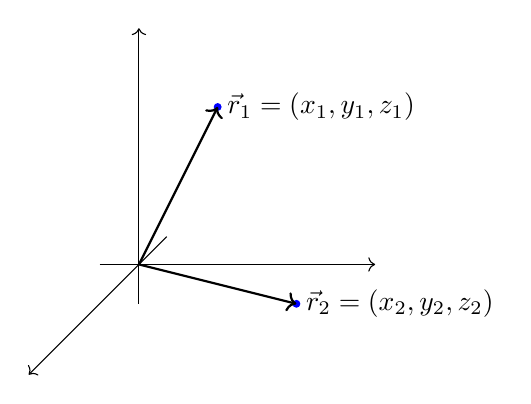
\begin{tikzpicture}[scale=1.0]
        % axis
        \draw[->] (-0.5,0) -- (3, 0);
        \draw[->] (0,-0.5) -- (0, 3);
        \draw[->] (0.353, 0.353) -- (-1.4, -1.4);
    
        \fill[blue] (2,-0.5) circle (0.05);
        \fill[blue] (1, 2) circle (0.05);
        \draw[->, thick] (0,0) -- (2, -0.5);
        \draw[->, thick] (0,0) -- (1, 2);
    
        \node[right] at (1,2) {$\vec r_1 = (x_1, y_1, z_1)$};
        \node[right] at (2,-0.5) {$\vec r_2 = (x_2, y_2, z_2)$};
    
    \end{tikzpicture}
    \caption{两体示意图}
    \end{figure}
% 2022-10-31 08:40:40  Wenbin Fan @FDU
设二者的坐标
\begin{align}
    &\vec r_1 = x_1 \vec i + y_1 \vec j + z_1 \vec k, \\
    &\vec r_2 = x_2 \vec i + y_2 \vec j + z_2 \vec k,
\end{align}
因此二者之间距离
\begin{align}
    \vec r &= \vec r_2 - \vec r_1 \\
    &= (x_2 - x_1) \vec i + (y_2 - y_1) \vec j + (z_2 - z_1) \vec k\\
    &=x \vec i + y \vec j + z \vec k,
\end{align}
引入了没有下标的坐标。

原子核和电子之间的力是库伦相互作用,
\begin{align}
    F = \frac{|e\times(-e)|}{r^2} = \frac{e^2}{r^2},
\end{align}
保守力(与路径无关的力)的势能为
\begin{align}
    V(r) = \int_r^\infty \frac{e^2}{r^2} \dd r = - \frac{e}{r},
\end{align}
对于氢原子,势能 $V(r) = -\frac{e^2}{r}$,类氢离子 $V(r) = - \frac{Z \ee^2}{r}$,其中 $Z$ 是核电荷数。

哈密顿算符
\begin{align}
    \hat H &= \hat T + \hat V \\
    &= -\frac{\hbar^2}{2m_1} \left(
        \pdv[2]{x_1} + \pdv[2]{y_1} + \pdv[2]{z_1}
    \right) 
    - \frac{\hbar^2}{2m_2} \left(
        \pdv[2]{x_2} + \pdv[2]{y_2} + \pdv[2]{z_2}
    \right) \notag\\
    &\phantom{=} + V\left(
        |\vec r_1 - \vec r_2|
        \right)
\end{align}
% 2022-10-31 08:54:24  Wenbin Fan @FDU
\courseTime{2 of 4, week 7}
将哈密顿量作用到波函数上
\begin{align}
    \hat H \psi(\vec r_2, \vec r_1) = E \psi (\vec r_2, \vec r_1)
\end{align}
\chat{%
只有可分离的两个变量才可以求解,希望可以分离变量。尝试坐标变换,将两个坐标变换成一个坐标,那么有可能求解。
}
考虑质心坐标,这是个很自然的拓展,想到这一步应该不难。质心坐标
\begin{align}
    \vec R = (X,Y,Z) = X \vec i + Y \vec j + Z \vec k,
\end{align}
那么坐标可表示为
\begin{align}
    X = \frac{m_1 x_1 + m_2 x_2}{M}, \quad Y = \frac{m_1 y_1 + m_2 y_2}{M}, \quad
    Z = \frac{m_1 z_1 + m_2 z_2}{M}
\end{align}
其中 $M = m_1 + m_2$。如果 $m_1 = m_2$,质心坐标便是平均坐标。相对坐标
\begin{align}
    \vec r = (x,y,z) = x \vec i + y \vec j + z \vec k,
\end{align}
其中分量为
\begin{align}
    x = x_2 - x_1, \quad y = y_2 - y_1, \quad z= z_2-z_1,
\end{align}
做变量代换
\begin{align}
    \begin{cases}
        x_1, y_1, z_1\\
        x_2, y_2, z_2
    \end{cases}
    \Rightarrow 
    \begin{cases}
        X,Y,Z\\
        x,y,z
    \end{cases}
\end{align}
% 【讨论】
变换成质心运动和相对运动。

坐标偏导
\begin{align}
    &\pdv{\psi}{x_1} = \pdv{\psi}{X} \pdv{X}{x_1} + \pdv{\psi}{x}\pdv{x_1}{x} =
    \left(\frac{m_1}{M} \pdv{x} - \pdv{x}\right)\psi, \\
    &\pdv[2]{\psi}{x_1} = 
    \left[
        \left(\frac {m_1}M\right)^2 \pdv[2]{X} - \frac{2m_1}{M} \pdv[2]{}{X}{x} + \pdv[2]{x}
    \right]\psi,
    \\
    &\pdv[2]{\psi}{x_2} = 
    \left[
        \left(\frac {m_2}M\right)^2 \pdv[2]{X} + \frac{2m_2}{M} \pdv[2]{}{X}{x} + \pdv[2]{x}
    \right]\psi,
\end{align}
同理由 $y$ 的坐标偏导
\begin{align}
    &\pdv[2]{\psi}{y_1} = 
    \left[
        \left(\frac {m_1}M\right)^2 \pdv[2]{Y} - \frac{2m_1}{M} \pdv[2]{}{Y}{y} + \pdv[2]{y}
    \right]\psi,
    \\
    &\pdv[2]{\psi}{y_2} = 
    \left[
        \left(\frac {m_2}M\right)^2 \pdv[2]{Y} + \frac{2m_2}{M} \pdv[2]{}{Y}{y} + \pdv[2]{y}
    \right]\psi,
\end{align}
\begin{align}
    &\pdv[2]{\psi}{z_1} = 
    \left[
        \left(\frac {m_1}M\right)^2 \pdv[2]{Z} - \frac{2m_1}{M} \pdv[2]{}{Z}{z} + \pdv[2]{z}
    \right]\psi,
    \\
    &\pdv[2]{\psi}{z_2} = 
    \left[
        \left(\frac {m_2}M\right)^2 \pdv[2]{Z} + \frac{2m_2}{M} \pdv[2]{}{Z}{z} + \pdv[2]{z}
    \right]\psi,
\end{align}
对于动能算符,最重要的是,我们希望变换到质心坐标
\begin{align}
    \frac1{m_1} \hat \nabla_2^2 + \frac1{m_2} \hat \nabla_2^2  = \frac1M \hat \nabla_M + \frac1{\mu} \hat \nabla_\mu,
\end{align}

合并含有 $M$ 的项,
\begin{multline}
    \frac 1{m_1} 
    \left(\frac{m_1}M\right)^2
    \left(
        \pdv[2]{X} + \pdv[2]{Y} + \pdv[2]{Z}
    \right) 
    + \frac1{m_2} 
    \left(\frac{m_2}M\right)^2 
    \left(
        \pdv[2]{X} + \pdv[2]{Y} + \pdv[2]{Z}
    \right) \\
     = \frac{m_1 + m_2}{M} \left(
        \pdv[2]{X} + \pdv[2]{Y} + \pdv[2]{Z}
     \right) = \frac1M \hat \nabla_M^2,
\end{multline}

以上二阶偏导中的第二项,除以各自质量后,耦合项全部相加抵消了。

合并二阶偏导中的第三项,
\begin{multline}
    \frac1{m_1} \left(\pdv[2]x + \pdv[2]y + \pdv[2]z\right) +
    \frac1{m_2} \left(\pdv[2]x + \pdv[2]y + \pdv[2]z\right) \\
    = \frac{m_1 + m_2}{m_1 m_2} \left(
        \pdv[2]x + \pdv[2]y + \pdv[2]z
    \right) = \frac{1}{\mu} \hat \nabla_\mu,
\end{multline}
这里正式引入了\boldtext{折合质量},
\begin{align}
    \mu = \frac{m_1m_2}{m_1 + m_2}, \quad \frac1{\mu}=\frac1{m_1} + \frac1{m_2}. 
\end{align}
氢原子的折合质量
\begin{align}
    \mu_{\mathrm H} = \frac{m_{\mathrm e} m_{\mathrm e}}{m_{\mathrm e}+m_{\mathrm e}} = \frac {m_{\mathrm e}} {1 + \frac{m_{\mathrm e}}{m_{\mathrm p}}} = \frac{m_{\mathrm e}}{1 + \num{5.45E-4}} = \num{0.99946} \,m_{\mathrm e}, 
\end{align}
通过折合质量,分离了整体运动和相对运动。因为原子核和电子的质量相差 3 个数量级,$1 \,m_{\mathrm p} = 1836 \,m_{\mathrm e}$。

重新写哈密顿算符,
\begin{align}
    \hat H &= \frac{\hat p_1^2}{2m_1} + \frac{\hat p_2^2}{2m_2} + V (|\vec r_1 - \vec r_2 |) \\
    &= \frac{\hat p_M^2}{2M} + \frac{\hat p_m^2}{2m} + V(x,y,z)
    \label{eq:hydro_cent_h}
\end{align}

\suppInfo{偏导数}{
还需要讲一点,变量代换后的偏导,
\begin{align}
    F(x,y) = F(f_1,f_2), \quad f_1=f_1(x,y), f_2=f_2(x,y),
\end{align}
其中的偏导
\begin{align}
    \pdv{F}{x} &= \left(\pdv{F}{f_1}\right)_{f_2} 
    \left[
        \left(\pdv{f_1}{x}\right)_y \pdv{x}{x}
        + \left(\pdv{f_1}{y}\right)_x \pdv{y}{x}
    \right] \notag\\
    &\phantom{=}
    +
    \left(\pdv{F}{f_2}\right)_{f_1}
    \left[
        \left(\pdv{f_2}{x}\right)_y \pdv{x}{x}
        + \left(\pdv{f_2}{y}\right)_x \pdv{y}{x}
    \right] 
\end{align}
如果 $x,y$ 线性无关,那么 $\pdv{y}{x} = 0$、$\pdv{x}{x} = 1$。
}
\chat{%
在求上面一系列二阶偏导的时候,我们不加证明地利用了
\begin{align}
    \pdv{x_1} \pdv{\psi}{X} = \pdv{X} \pdv{\psi}{x_1},
\end{align}
实际上背后隐藏的是
\begin{align}
    &\left[
        \pdv{x_1}, \pdv{X}
    \right] = 0, \\
    & [\hat \nabla_1, \hat \nabla\!_M] = 0,\\
    &[\hat \nabla_1, \hat \nabla\!_\mu] = 0,
\end{align}
}

当哈密顿量写成质心和相对运动时,\eqref{eq:hydro_cent_h} 继续写成
\begin{align}
    \hat H = -\frac{\hbar^2}{2m} \hat \nabla_M^2 -
    -\frac{\hbar^2}{2m} \hat \nabla_\mu^2 + V(r),
\end{align}
相对运动包含了相互作用势能。

% 与之前有什么不一样?【】【】
% 2022-10-31 09:29:46  Wenbin Fan @FDU
\chat{%
很多内容需要深入思考。本课是物化的扩展,更深入地讲解理论知识。希望本课的推导,能帮助同学们理解知识点。
}

\section{中心力场}
这是一个\boldtext{中心力场}的问题,
\begin{align}
    \psi_{\mathrm{tot}} = \psi_{\mathrm{tr}}(x,y,z) \,\psi_(x,y,z),
\end{align}
可以天然地分离成整体和相对运动的波函数,将其代入薛定谔方程,
\begin{align}
    \left[
        -\frac{\hbar^2}{2M}\hat\nabla_M^2 - \frac{\hbar^2}{2m} \hat\nabla_\mu^2 + V(r) 
    \right] \psi_{\mathrm{tr}} \psi = E \psi_{\mathrm{tr}} \psi
\end{align}
整理得到
\begin{align}
    - \frac{\hbar^2}{2M}\hat\nabla_M^2 \psi_{\mathrm{tr}} = \psi_{\mathrm{tr}} \left[
        E + \frac{\hbar^2}{2\mu}\hat\nabla_\mu^2 - V(r)
    \right]\psi
\end{align}
两边同时除以整体波函数
\begin{align}
    -\frac{\hbar^2}{2m} \frac1{\psi_{\mathrm{tr}}} \hat\nabla_M^2 \psi_{\mathrm{tr}} = \frac1{\psi} \left[
        E + \frac{\hbar^2}{2\mu}\hat\nabla_\mu^2 - V(r)
    \right]\psi
\end{align}
左边只与整体运动有关,右边只与相对运动有关,因此波函数可以分成两部分,
\begin{align}
    & - \frac{\hbar^2}{2m} \hat \nabla_m \psi_{\mathrm{tr}} = E_\mathrm{tr} \psi_{\mathrm{tr}}, 
    \label{eq:hydro_Htr}
    \\
    & \left[-\frac{\hbar^2}{2m} \hat\nabla_\mu^2 + V(x,y,z)\right] \psi = E_\mathrm{int} \psi
    \label{eq:hydro_Hint}
    角度部分\end{align}
其中,系统整体能量 $E = E_{\mathrm{tr}} + E_{\mathrm{int}}$。平动能 $E_{\mathrm{tr}}$ 用 $K$ 表示,便于后面写。

平动的求解,类比自由粒子,
\begin{align}
    -\frac{\hbar^2}{2m} \hat\nabla_\mu^2 \psi + V(x,y,z) \psi = E_\mathrm{int} \psi, 
\end{align}

\homework{\textbf{7.1}  对于3个粒子的体系,约化质量后的 $\hat H$ 能否分离变量,$N$ 个粒子呢?为什么要引入 Born--Oppenheimer 近似?}
举个简单的粒子,三粒子可以用 He 原子或氢分子离子来理解,那么能否分离变量呢?下午讲。

\courseTime{OCT31 2022 下午}
动能算符
\begin{align}
     \hat \nabla^2_\mu = \pdv[2]x + \pdv[2]y + \pdv[2]z = \pdv[2]r + \frac2r \pdv{r} - \frac1{\hbar^2r^2} \hat L^2 (\theta, \psi), 
\end{align}
其中
\begin{align}
    \hat L^2 = -\hbar^2 \left(
        \frac1{\sin^2\theta} \pdv[2]{\psi} + \cot\theta \pdv{\theta} + \pdv[2]\theta
    \right). 
\end{align}
上周已经求了
\begin{align}
    \hat L^2 Y_l^{m_l} = \hbar^2 \,l(l+1) Y_l^{m_l}(\theta,\varphi), 
\end{align}
【】
设
\begin{align}
    \Phi(r,\theta,\varphi) = R(r) Y_l^{m_l} (\theta,\varphi),
\end{align}
提出与角度无关的部分
\begin{multline}
    -\frac{\hbar^2}{2m} 
    \left[
    Y_l^{m_l} (\theta,\varphi) \left(\pdv[2]r + \frac2r \pdv{r}\right) R(r) - \frac{R(r)}{\hbar^2r^2} \hat L^2 Y_l^{m_l} (\theta,\varphi)
    \right] \\
    + V(r) R(r) Y_l^{m_l} (\theta, \varphi) = E_{\mathrm {int}}\psi,
\end{multline}
两边同时除以波函数,得到
\begin{multline}
    -\frac{\hbar^2}{2m} \frac1{R(r)} 
    \left(\pdv[2]r + \frac2r \pdv{r}\right) R(r)  \\ + \frac1{2\mu r^2} \frac1{Y_l^{m_l}(\theta,\varphi)} \hat L^2 \frac1{Y_l^{m_l}(\theta,\varphi)}  = E_{\mathrm{int}} - V(r)
\end{multline}
第一项与角度无关,但是第二项里有个 $\frac1{r^2}$,争取把第二项变成与 $r$ 无关的项。继续化简,
\begin{align}
    &\text{LHS} = -\frac{\hbar^2}{2m} \frac{r^2}{R(r)} 
    \left(\pdv[2]r + \frac2r \pdv{r}\right) R(r) - (E_{\mathrm{int}} - V(r)) r^2, \\
    &\text{RHS} = -\frac1{2\mu} \frac1{Y_l^{m_l}} \hat L^2 Y_l^{m_l}(\theta,\varphi),
\end{align}
左边与径向有关,右边与角度有关,因此二者都等于常数 $\text{LHS} = \text{RHS} = K$。

角度相关项,
\begin{align}
    \hat L^2 Y_l^{m_l} (\theta,\varphi) &= 2 \mu K Y_l^{m_l} (\theta,\varphi) \\
    &= \hbar^2 \,l(l+1) Y_l^{m_l} (\theta,\varphi),
\end{align}
解出来
\begin{align}
    K = - \frac{\hbar^2 l(l+1)}{2\mu},
\end{align}
那么把 $K$ 代回径向部分,
\begin{align}
    -\frac{\hbar^2}{2\mu} r^2 \left(\pdv[2]r + \frac2r \pdv{r}\right) R(r) - [ E_{\mathrm{int}} - V(r)] r^2 R(r) = 
    - \frac{\hbar^2 l(l+1)}{2\mu} R(r)
\end{align}
把左边的 $r^2$ 除到右边去,整理可得
% 2022-10-31 13:46:43  Wenbin Fan @FDU
% 随时可以提问
\begin{align}
    -\frac{\hbar^2}{2\mu} \left(\pdv[2]r + \frac2r \pdv{r}\right) R(r)
    + \left[
        \frac{\hbar^2 l(l+1)}{2\mu} + V(r)
    \right] R(r)
    = 
    E_{\mathrm{int}} R(r),
\end{align}
我们更偏好最高阶项没有系数,
\begin{align}
    \left(\pdv[2]r + \frac2r \pdv{r}\right) R(r) 
    + \left\{
        - \frac{l(l+1)}{r^2} + \frac{2\mu}{\hbar^2} 
        \left[
            E_{\mathrm{int}} - V(r)
        \right] 
    \right\} R(r) = 0,
\end{align}

\section{径向部分的求解}
\begin{figure}[tp]\centering
    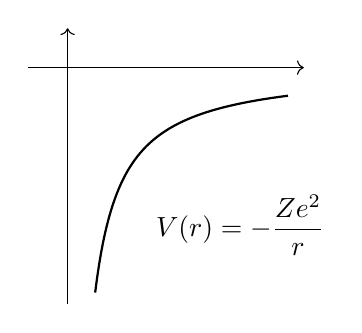
\begin{tikzpicture}[scale=1.0]
        % axis
        \draw[->] (-0.5,0) -- (3, 0);
        \draw[->] (0,-3) -- (0, 0.5);
    
        \draw[domain=0.35:2.8,thick,samples=100] plot (\x,{-1/\x});
        \node[right] at (1,-2) {$V(r) = -\displaystyle\frac{Ze^2}{r}$};
    
    \end{tikzpicture}
    \caption{氢原子中的吸引势}
    \label{fig:H_attraction}
    \end{figure}
势函数如图 \ref{fig:H_attraction}。当两体接近时,势能趋于 $-\infty$。如果能量 $E>0$ 表示 $T>0>V$,解离态。只有当能量 $E<0$ 才表示束缚态,仅考虑这种情况。

上面方程里的系数太多了,做变量代换,目的是为了凑成已知的微分方程。令
\begin{align}
    a^2 = -\frac{2\mu E_{\mathrm{int}}}{\hbar^2}, \quad 
    a = \frac{\sqrt{2\mu E_{\mathrm{int}}}} {\hbar}, 
\end{align}
那么从 $E$ 的量子化,变成了 $a$ 的量子化,重写方程,
\begin{align}
    R''(r) + \frac2r R'(r) + \left[
        -a^2 + \frac{2\mu}{\hbar^2} \frac{Ze^2}{r} - \frac{l(l+1)}{r^2}
    \right] R(r) = 0, \label{eq:hydro_quantized_a}
\end{align}
我们不喜欢中括号中间一项,如果有它,方程的解会变得很复杂。利用\boldtext{坐标缩放},尝试消去它。定义 $\rho = kr$,接下来推导 $k$ 为何值时可以消去。则 $R(r) = R(\rho)$,偏导为
\begin{align}
    \pdv{R(\rho)}{r} = \pdv{R(\rho)}{\rho} \pdv{\rho}{r} = k \pdv{R(\rho)}{\rho}, \quad \pdv[2]{R(\rho)}{r} 
    = k^2 \pdv[2]{R(\rho)}{\rho}
\end{align}
\begin{lstlisting}
D[R[k r], {r, 2}] /. {r -> \[Rho]/k}
>> k^2 (R^\[Prime]\[Prime])[\[Rho]]
\end{lstlisting}
那么 \eqref{eq:hydro_quantized_a} 变换成了
\begin{align}
    k^2 R''(\rho) + \frac{2k}{\rho/k} R'(\rho) + \left[
        -a^2 + \frac{2\mu}{\rho} \frac{Ze^2k}{\rho} - \frac{l(l+1)k^2}{\rho^2}
    \right] R(\rho) = 0
\end{align}
约掉高次项的 $k^2$。此时注意到,当 $k=2a$ 时,有
\begin{align}
    R''(\rho) + \frac2{\rho} R'(\rho) + \left[
        \frac14 + \frac{\lambda}{\rho} - \frac{l(l+1)}{\rho^2}
    \right] R(\rho) = 0
\end{align}
现在方程就简单一些了。

按照经验,我们先求解渐近形式。当 $\rho \rightarrow \infty$ 时,
\begin{align}
    R''(\rho) - \frac14 R(\rho) = 0
\end{align}
解得 $R(\rho) = \ee^{\rho/2}$(舍去)或 $R(\rho) = \ee^{-\rho/2}$,那么
\begin{align}
    R(\rho) = \ee^{-\rho/2} F(\rho),
\end{align}

代回去,直接给出结果
\begin{align}
    \pdv[2]{F(\rho)}{\rho} + \left(\frac2\rho -1\right) \pdv{F(\rho)}{\rho} + \left(
        \frac\lambda\rho - \frac{l(l+1)}{\rho^2} - \frac1\rho
    \right) F(\rho) = 0,
\end{align}
发现,当 $\rho\rightarrow 0$时有奇点,导致 $F(\rho)$ 不能在 $\rho = 0$ 直接展开。
% 为啥这么定义 F?下面的式子 % 2022-10-31 14:05:21  Wenbin Fan @FDU
定义
\begin{align}
    F(\rho) = \rho^n L(\rho), \quad L(\rho) = \sum_{k=0}^\infty a_k \rho^k, \quad a_0\neq0
\end{align}
称作广义幂级数 generalized power series。有
\begin{align}
    &F'(\rho) = n\rho^{n-1} L(\rho) + \rho^n L'(\rho), \\
    &F''(\rho) = n(n-1) \rho^{n-1} L(\rho) + 2n\rho^{n-1} L'(\rho) 
    + \rho^n L''(\rho),
\end{align}
把导数代回去,有
\begin{multline}
    \rho^n L ''(\rho) + 2n \rho^{n-1} L'(\rho) + n(n-1) \rho^{n-2} L(\rho) + \\
    \left(\frac2\rho -1\right)
    \left[
        n\rho^{n-1} L(\rho) + \rho^n L'(\rho)
    \right]\\
    + \left[
        \lambda \rho^{n-1} - l(l+1) \rho^{n-2} - \rho^{n-1}
    \right] L(\rho) = 0,
\end{multline}
合并同类项,
\begin{multline}
    \rho^n L''(\rho) +( 2n \rho^{n-1} - 2\rho^{n-1} - \rho^n) L'(\rho) + \\
    \left\{
    [n(n+1) - l (l+1)] \rho^{n-2} + (\lambda - 1-n) \rho^{n-1}
    \right\} L(\rho) = 0,
\end{multline}
两边同除 $\rho^{n-2}$,
\begin{multline}
    \rho^2 L''(\rho) +( 2n \rho^{n-1} - 2\rho^{n-1} - \rho^n) L'(\rho) + \\
    \left\{
    [n(n+1) - l (l+1)] + (\lambda - 1-n)\rho
    \right\} L(\rho) = 0,
\end{multline}
如果要消奇点,我们发现,当 $\rho \rightarrow 0$时,衰减最慢的是 $[n(n+1) - l (l+1)] L(\rho) = 0$,所以要求这一项为 0,解得 $n=l$,舍去负数解。
\courseTime{week7, 4 of 4}

得到了
\begin{align}
    F(\rho) = \rho^l L(\rho),
\end{align}
那么
\begin{align}
    \rho L''(\rho) + [2(l+1) -\rho]L'(\rho) + (\lambda - 1 -l) L(\rho) = 0, \label{eq:hydro_L_initial_def}
\end{align}
对 $L$ 做级数展开,刚才定义过了,
\begin{align}
    L(\rho) = \sum_{k=0}^\infty a_k \rho^k, \quad a\neq 0,
\end{align}
合并归类相同级数,
\begin{align}
    (\lambda - l - 1 - k)a_k + 
    \left[
        2(k+1) (l+1) + k(k+1)
    \right] a_{k+1} = 0
\end{align}
得到了递推条件
\begin{align}
    \frac{a_{k+1}}{a_k} = \frac{2(k+1) (l+1) + k(k+1)} {\lambda - l - 1 - k}
\end{align}
这里为什么是间隔是 1?极坐标下的动能算符是一阶的。

当 $k\rightarrow\infty$ 是,系数的间隔
\begin{align}
    \frac{a_{k+1}}{a_k} \sim \frac{k}{k^2} = \frac1{k},
\end{align}
指数的间隔
\begin{align}
    \ee^\rho = 1 + \frac{\rho}{1!} + \frac{\rho^2}{2!} + \cdots + \frac{\rho^k}{k!} + \cdots,
\end{align}
同样有
\begin{align}
    \frac{a_{k+1}}{a_k} = \frac{k!}{(k+1)!} \sim \frac1{k}. 
\end{align}
因此,当 $k\rightarrow\infty$ 时,
\begin{align}
    R(\rho) = \ee^{-\rho/2} \rho^l \ee^{\rho} = \rho^l \ee^{\rho/2}
\end{align}
发散,所以必须截断。由 $k+l+ = \lambda$,定义\boldtext{主量子数}。$n=l+1, l+2, \cdots$,因为 $l=0,1,2,3,\cdots$,$n$ 允许的取值是 $1,2,3,\cdots$。

氢原子的能级 $n = \lambda = \frac{\mu Z \ee^2}{\hbar a}$,代入 $a$ 的定义有
\begin{align}
    E_{\mathrm{int}} = -\frac{\hbar^2a^2}{2\mu} = - \frac{\mu^2 \ee^4} {2\hbar^2 n^2} = - R\frac{Z^2}{n^2},
\end{align}
式子中
\begin{align}
    R = \frac{\mu^2e^2}{2\hbar^2} = \SI{13.6}{\electronvolt},
\end{align}
称为\boldtext{里德堡} \boldtext{Rydberg 常数}。
因此从截断条件得到了量子化条件、能级。为什么 $n\neq 0$?如果 $n=0$,能量无穷大。

随着主量子数增大,能级间隔越来越小,
\begin{align}
    \frac1\lambda = \frac{\Delta E}{\hbar^2} = R Z^2 \left(
        \frac1{n_1^2} - \frac1{n_2^2}
    \right). 
\end{align}

% 2022-10-31 14:39:24  Wenbin Fan @FDU
径向波函数
\begin{align}
    R_n^l (r) = A \ee^{- \rho/2} \rho^l L_n^l(\rho), \quad \rho = 2ar,
    \quad a = \frac{\mu Z \ee^2}{\hbar^2 n} = \frac Z{na_0},
\end{align}
其中
\begin{align}
    a_0 = \frac{\hbar^2}{\mu \ee^2} = \SI{52.9}{\pico\metre} = \SI{0.529}{\angstrom}
\end{align}
称作\boldtext{波尔半径} Bohr radius。最终写作
\begin{align}
    R_{n,l}(r) = N r^l \ee^{- \frac{Zr}{na_0}} \sum_{k=0}^{n-l-1} b_k r^k,
\end{align}
其中 $N$ 是归一化系数。
\homework{\textbf{7.2} 求这个归一化系数。}

我们最开始求解的是 \eqref{eq:hydro_L_initial_def}
,它与连带拉盖尔方程是同样的形式。因此各项相等,有
\begin{align}
    & x = \rho, \\
    & a = 2l+1,\\
    &\nu = n-l-1,
\end{align}

% 拉盖尔方程有多种形近的定义,这里给出徐光宪、范康年等各自书中的定义,
% \begin{align}
%     L_{\nu+\alpha}^l (x) = \sum{k=0}^{\nu}
%     \frac{(-1)^{k+m} (\nu+a)!(\nu+a)!}{[][][]}
% \end{align}
% 还有微分定义,
% \begin{align}
%     [][]
% \end{align}
% 【一大段公式】
\suppInfo{连带Laguerre多项式的定义}{
    至少有两种定义。定义一:顾樵、Wikipedia、Mathematica。级数定义($ \alpha = 2l+1$, $\nu = n-l-1 $)
    \begin{equation}\label{poly}
    L_\nu^\alpha(x) = (\nu + \alpha)! \sum_{k=0}^\nu \dfrac{(-1)^k}{k!(\nu-k)!(k+\alpha)!} x^k
    \end{equation}
    递推关系
    \begin{equation}\label{recur}
    L_{\nu+1}^\alpha (x) = \dfrac{(2\nu+1+\alpha-x) L_\nu^\alpha(x) - (\nu+\alpha) L_{\nu-1}^\alpha(x)}{\nu+1}
    \end{equation}
    微分表示
    \begin{align}\label{diff}
    &L_\nu^\alpha (x) = (-1)^\alpha \pdv[\alpha]{x} L_{\nu+\alpha}(x) , \\
    &L_{\nu+\alpha}(x) = \dfrac{e^x}{(\nu+\alpha)!} \pdv[\nu]{x}(e^{-x} x^{\nu+\alpha})
    \end{align}
    $ L_n(x) $称为Laguerre函数。
    Rodrigues公式
    \begin{equation}\label{rodr}
    L_\nu^\alpha (x) = \dfrac{x^{-\alpha} \ee^x  }{\nu!} \pdv[\nu]{x}(e^{-x} x^{\nu+\alpha})
    \end{equation}

    定义二:徐光宪、范康年。
    级数定义($ \alpha = 2l+1, \nu' = n+l $)
    \begin{equation}\label{poly2}
    \tilde L_{\nu'}^\alpha(x) = \sum_{k=0}^{\nu'-\alpha} \dfrac{(-1)^{k+m} \nu'!\nu'!}{(\nu'-\alpha-k)!(k+\alpha)!k!} x^k
    \end{equation}
    注意到$ \nu' = \nu + \alpha $
    \begin{align}
    \tilde L_{\nu'}^\alpha(x) &= (\nu+\alpha)! (\nu+\alpha)! \sum_{k=0}^{\nu} \dfrac{(-1)^{k+m}}{(\nu-k)!(k+\alpha)!k!} x^k 
    \end{align}
    所以定义二和定义一相差一个倍数
    \begin{equation}\label{key}
    \tilde L_{\nu'}^\alpha(x) = (-1)^m (\nu+\alpha)! L_\nu^\alpha(x)
    \end{equation}
    微分表示
    \begin{equation}\label{diff2}
    \tilde L_{\nu'}^\alpha (x) = \pdv[\alpha]{x} L_{\nu'}(x) , \quad \tilde L_{\nu'}(x) = \ee^x \pdv[\nu']{x}(e^{-x} x^{\nu'})
    \end{equation}
    %Rodrigues公式
    %\begin{equation}\label{key}
    %L_\nu^\alpha (x) = \dfrac{x^{-\alpha} \ee^x  }{\nu!} \pdv[\nu]{x}(e^{-x} x^{\nu+\alpha})
    %\end{equation}
    参考徐光宪 \S 3.4;顾樵 \S 8.3.2。
}

写出径向波函数的最终表达式,
\begin{align}
    R_{n,l} (r) = N \ee^{-\rho/2} \rho^l L^{2l+1}_{n+l}(\rho), 
    \quad N^2 = \left(\frac{2Z}{na_0}\right)^3 \frac{(n-l-1)!}{2n[(n+l)!]^3},
\end{align}
% 2022-10-31 14:54:11  Wenbin Fan @FDU
当 $n = 1$、$l=0$ 时,
\begin{align}
    L_1^1 (\rho) = \dv{\rho} \left[
        \ee^{\rho} \dv{\rho} (\ee^{-\rho}\rho)
    \right] = -1,
\end{align}
\begin{lstlisting}
D[Exp[r] D[Exp[-r] r, r], r] // Simplify
>> -1
\end{lstlisting}
所以
\begin{align}
    R_{1,0} (r) = 2 \left(\frac Za\right)^{3/2} \ee^{-Zr/a}. 
\end{align}
% 有几行没拍
\homework{\textbf{7.3} (选做)写一个生成连带拉盖尔多项式的程序,要求 $n,l$ 为输入。}

\section{类氢离子}
类氢离子的波函数
\begin{align}
    \Psi_{n,l,m_l}(r,\theta,\varphi) = R_{n,l}(r) \Theta_{l,m_l}(\theta) \Phi_{m_l}(\phi).
\end{align}

主量子数 $n$ 唯一确定能量,对于任意 $n$ 都有 $\sum_{l=0}^{n-1} (2l+1) = n^2$ 个角动量。

化学中,对不同的角动量有不同的名字,即。
\begin{table}[ht]
    \centering
    % \caption{Thicker horizontal lines above and below the table.}
    \begin{tabular}[t]{ccccccc}
    \toprule
    主量子数 & 1&2&3&4&5&6\\
    \midrule
    光谱记号 & s&p&d&f&g&h\\
    \bottomrule
    \end{tabular}
    \caption{主量子数与光谱记号}
    \end{table}%

    列举一些具体的波函数
    % 1s, 2s,2\mathrm{p}(1,0,-1)}
    \begin{align}
    \Psi_{1\mathrm{s}} &= \dfrac{1}{\sqrt{\pi}} \qty(\dfrac{Z}{a_0})^{3/2} \ee^{-Zr/a_0} \\
    \Psi_{2\mathrm{s}} &= \dfrac{1}{4\sqrt{2\pi}} \qty(\dfrac{Z}{a_0})^{3/2} \qty(2-\dfrac{Zr}{a_0}) \ee^{-Zr/2a_0}
    \end{align}
    \begin{align}
    \Psi_{2\mathrm{p}_{+1}} &= \dfrac{1}{8\sqrt{\pi}} \qty(\dfrac{Z}{a_0})^{3/2}  \dfrac{Zr}{a_0} \ee^{-Zr/2a_0} \sin\theta \,\ee^ {\ii\phi} \\
    \Psi_{2\mathrm{p}_0} &= \dfrac{1}{4\sqrt{2\pi}} \qty(\dfrac{Z}{a_0})^{3/2}  \dfrac{Zr}{a_0} \ee^{-Zr/2a_0} \cos\theta \\
    \Psi_{2\mathrm{p}_{-1}} &= \dfrac{1}{8\sqrt{\pi}} \qty(\dfrac{Z}{a_0})^{3/2}  \dfrac{Zr}{a_0} \ee^{-Zr/2a_0} \sin\theta \,\ee^ {-\ii\phi}
    \end{align}
    转化为实函数
    \begin{align}
    \Psi_{2\mathrm{p}_x} &= \dfrac{1}{\sqrt{2}}( \Psi_{2\mathrm{p}_{+1}} + \Psi_{2\mathrm{p}_{-1}}) \\
    &= \dfrac{1}{4\sqrt{2\pi}} \qty(\dfrac{Z}{a_0})^{3/2}  \dfrac{Zr}{a_0} \ee^{-Zr/2a_0} \sin\theta\cos\phi\\
    \Psi_{2\mathrm{p}_z} &= \Psi_{2\mathrm{p}_0}\\
    \Psi_{2\mathrm{p}_y} &=  \dfrac{1} {\ii\sqrt{2}}( \Psi_{2\mathrm{p}+1} - \Psi_{2\mathrm{p}-1}) \\
    &=\dfrac{1}{4\sqrt{2\pi}} \qty(\dfrac{Z}{a_0})^{3/2}  \dfrac{Zr}{a_0} \ee^{-Zr/2a_0} \sin\theta\sin\phi 
    \end{align}
    事实上$ x,y,z $记号来自于
    \begin{align}
    \Psi_{2\mathrm{p}_x} &=  \dfrac{1}{4\sqrt{2\pi}} \qty(\dfrac{Z}{a_0})^{3/2}  \dfrac{Z}{a_0} x\, \ee^{-Zr/2a_0} \\
    \Psi_{2\mathrm{p}_z} &= \dfrac{1}{4\sqrt{2\pi}} \qty(\dfrac{Z}{a_0})^{3/2}  \dfrac{Z}{a_0} z\, \ee^{-Zr/2a_0}\\
    \Psi_{2\mathrm{p}_y} &= \dfrac{1}{4\sqrt{2\pi}} \qty(\dfrac{Z}{a_0})^{3/2}  \dfrac{Z}{a_0} y\, \ee^{-Zr/2a_0} 
    \end{align}
    参考 Levine \S 6.6

画图的时候,一般是画 $\mathrm{p}_x, \mathrm{p}_y, \mathrm{p}_z$,因为 $\mathrm{p}_{-1}$ 等有虚部。
% 我们对 p 轨道进行线性组合,
% % \begin{align}
% %     2\mathrm{p}_x = \frac1{\sqrt2} (2\mathrm{p}_{-1} + 2\mathrm{p}_{+1}) = [][]
% % \end{align}
% 实际上我们发现,$r \,\sin\theta\,\cos\varphi = x$,这也是它们称之为 $xyz$ 的原因,相当于投影。

\homework{\textbf{7.4}  (a) 探讨实轨道 $\mathrm{p}_x, \mathrm{p}_y, \mathrm{p}_z$ 与复轨道 $\mathrm{p}_{-1}, \mathrm{p}_0, \mathrm{p}_1$ 的变换关系,(b) 分别画出 $\mathrm{p}_x, \mathrm{p}_y, \mathrm{p}_z$ 与 $\mathrm{p}_{-1}, \mathrm{p}_0, \mathrm{p}_1$ 轨道的图形,并进行比较。

\textbf{7.5}  画出 1s、2s、3s、3p、3d 轨道的径向函数($R(r)$-$r$)和径向分布函数($D(r)$-$r$)的图像。}

% 预告:第9次课、第 11 次课为上机。

\courseTime{Nov7 2022}
\section{复习}
总结前半学期的内容。

讲变分法。变分的原因是无法精确求解,用数值方法逼近。到这节课为止,之前的所有的体系(自由粒子、氢原子等等)都是可以精确求解的。现在复习以前的内容。

上半学期,由演绎和类比,得到量子力学的基本假设和框架。从原理上来说,本质上来说需要知道微观状态波函数。在一次量子化中可以由一次量子化求解薛定谔方程得到。因为哈密顿算符不含时,可分离得到静态薛定谔方程和含时部分。这门课里所有的体系都是围绕定态薛定谔方程展开的,
\begin{align}
    \hat H \psi_i = E_i \psi_i.
\end{align}

\textbf{一维单粒子}
\begin{align}
    \hat H = \hat T + \hat V = -\frac{\hbar^2}{2m} \pdv[2]x + V(x). 
\end{align}

1. 自由粒子  $V(x) = 0$

2. 单侧无限深势阱
$V(x) = \begin{cases}
    0, \quad &x\in(0,l),\\
    +\infty, \quad &\text{其它},
\end{cases}$

3. 单侧半无限深势阱 $V(x)=\begin{cases}
    0, \quad &x\in(0,l), \\
    V, \quad &x\in[l,\infty), \\
    +\infty, \quad &x\in(-\infty, 0], 
\end{cases}$

4. 有限深势阱 $V(x) = \begin{cases}
    V, \quad &x \notin (0,l), \\
    0, \quad &x\in(0,l)
\end{cases}$

尽管这些模型很简单,也有它实际的意义。求解薛定谔方程,由品优波函数的假设,可以得到量子化条件。

5. 谐振子 $V(x) = \frac12 kx^2$,最复杂的一维单粒子模型,用幂级数求解。

我们又介绍了\textbf{二维单粒子}体系,与一维的不同在于其中的动能算符变成了二维,
\begin{align}
    \hat T = \hat T + \hat V = -\frac{\hbar^2}{2m} \left(\pdv[2]x + \pdv[2]y\right) + V(x,y). 
\end{align}
我们求解了

6. 粒子在环上的运动 $V(x,y) = \begin{cases}
    0, \quad &\sqrt{x^2 + y^2} = R, \\
    +\infty, \quad &\sqrt{x^2+y^2} \neq R,
\end{cases}$
求解它,要将笛卡尔坐标变换到极坐标 $(x,y) \rightarrow (r,\theta)$。

很快我们就到了\textbf{三维单粒子}体系,其动能算符也相应地变成三维的,
\begin{align}
    \hat T &= -\frac{\hbar^2}{2m} \left(\pdv[2]x + \pdv[2]y + \pdv[2]z\right) + V(x,y,z) \\
    &= -\frac{\hbar^2}{2m} \left(
        \hat\nabla_x^2 + \hat\nabla_y^2 + \hat\nabla_z^2 
    \right) = -\frac{\hbar^2}{2m} \hat\nabla^2, 
\end{align}

7. 球面 $V(x,y,z) = \begin{cases}
    0, \quad &\sqrt{x^2 + y^2 + z^2} = R, \\
    +\infty, \quad&\text{其它},
\end{cases}$
分离变量 $(x,y,z) \rightarrow (r,\theta,\varphi)$。

\textbf{三维两体},此时哈密顿量与两体有关,其中动能
\begin{align}
    \hat H = \hat T + \hat V = -\frac{\hbar^2}2 \sum_i \frac{1}{m_i} \hat\nabla_i^2 + \hat V(\vec r_1, \vec r_2, \cdots, \vec r_n),
\end{align}

8. 类氢离子,粒子感受到的是库仑力
\begin{align}
    V(\vec r_1, \vec r_2) = - \frac{Z_2 e^2}{|\vec r_1 - \vec r_2|},
\end{align}
想要求解它,(1) 将两体的运动分离成整体和相对运动 $(x_1, y_1, z_1, x_2, y_2, z_2) \rightarrow (X,Y,Z, x,y,z)$,质量变换 $(m_1, m_2) \rightarrow (M, m)$,哈密顿算符成为了
\begin{align}
    \hat H = - \frac{\hbar^2}{2M} \left(
        \pdv[2]X + \pdv[2]Y + \pdv[2]Z
    \right) - \frac{\hbar^2}{2\mu}  \left(
        \pdv[2]x + \pdv[2]y + \pdv[2]z
    \right) + V(\vec r), 
\end{align}
势函数成为了相对坐标的函数。(2) 复杂的地方在于其中的相对运动部分,
\begin{align}
    \hat H = -\frac{\hbar^2}{2\mu}  \left(
        \pdv[2]x + \pdv[2]y + \pdv[2]z
    \right) + V(\vec r), 
\end{align}
通过求解球面体系,我们知道要利用坐标变换,把哈密顿量变换到极坐标下 $(x,y,z) \rightarrow (r,\theta,\phi)$。

到底什么体系才是可以精确求解的?微分方程的通解是\boldtext{闭合表示}。数学中的闭合表示指可以通过有限次操作完成。前面可以精确求解的体系,都是可以由哈密顿量求出闭合解,进而求解。

对于三体的问题,氢分子能否精确求解?
\begin{figure}[tp]\centering
    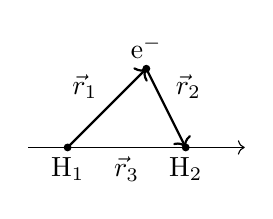
\begin{tikzpicture}[scale=0.5]
        \draw[->] (-3,0) -- (2.5, 0);
        \draw[->, thick] (-2,0) -- (0,2);
        \draw[->, thick] (0,2) -- (1,0);
        \node[below] at (-0.5,0) {$\vec r_3$};
        \node[above left] at (-1,1) {$\vec r_1$};
        \node[above right] at (0.5, 1) {$\vec r_2$};
    
        \fill (-2,0) circle (0.1);
        \fill (1,0) circle (0.1);
        \node[below] at (-2,0) {H$_1$};
        \node[below] at (1,0) {H$_2$};
        \fill (0,2) circle (0.1);
        \node[above] at (0,2) {e$^-$};
    \end{tikzpicture}
    \caption{氢分子示意图}
    \end{figure}

9. 氢分子,与氢原子唯一的不同是多了质子,
\begin{align}
    \hat H = - \frac{\hbar^2}{2m} \hat \nabla_1^2 - \frac{\hbar^2}{2m} \hat\nabla_2^2 - \frac{\hbar^2}{2m_\mathrm{e}} \hat \nabla_{\mathrm e}^2 + \frac{e^2}{r_3} - \frac{e^2}{r_1} - \frac{e^2}{r_2},
\end{align}
实际上它不可能通过坐标变换的方式分离三个变量。在 Born--Oppenheimer 近似下,将原子和电子运动分离开。

为什么不可以分离?三体是完全耦合的,数学上可以证明做不到。

分开原子核和电子的哈密顿量,其中电子的部分
\begin{align}
    \hat H = - \frac{\hbar^2}{2m} \hat\nabla_1^2 - \frac{\hbar^2}{2m} \hat\nabla_2^2 - \frac{\hbar^2}{2m_\mathrm{e}} \hat\nabla_{\mathrm{e}}^2 + \frac{e^2}{r_3} - \frac{e^2}{r_1} - \frac{e^2}{r_2},
\end{align}
三体全部两两耦合在一起,从数学角度不可能分离变量。因为原子核质量远大于电子质量,有三个数量级以上的差别,所以电子的运动会远远快于原子核。假设电子能迅速响应原子核位置的变化,或者假设原子核位置不动、将原子核坐标视为电子波函数的参数,从而分离原子核与电子的波函数,这称作 Born--Oppenheimer 近似。

分离之后,电子部分的哈密顿算符
\begin{align}
    \hat H = - \frac{\hbar^2}{2m_{\mathrm e}} \hat \nabla_\mathrm{e}^2 - \frac{e^2}{r_1} - \frac{e^2}{r_2},
\end{align}
它不能用简单的球谐函数求解,而是复杂的椭球函数。推荐文献 arXiv:quant-ph/0607081,给出了电子波函数的精确形式。

\begin{figure}[tp]\centering
    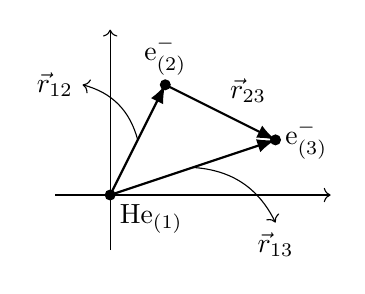
\begin{tikzpicture}[scale=0.7]
        \draw[->] (-1,0) -- (4,0);
        \draw[->] (0,-1) -- (0,3);
        
        \fill (0,0) circle (0.1);
        \fill (1,2) circle (0.1);
        \fill (3,1) circle (0.1);
    
        \draw[-Latex, thick] (0,0) -- (1,2);
        \draw[-Latex, thick] (0,0) -- (3,1);
        \draw[-Latex, thick] (1,2) -- (3,1);
    
        \node[below right] at (0,0) {He$_{(1)}$};
        \node[above] at (1,2) {e$^-_{(2)}$};
        \node[right] at (3,1) {e$^{-}_{(3)}$};
    
        \node[above right] at (2,1.5) {$\vec r_{23}$};
        \draw[->] (0.5,1) to [bend right] (-0.5, 2);
        \node[left] at (-0.5,2) {$\vec r_{12}$};
        \draw[->] (1.5,0.5) to [bend left] (3,-0.5);
        \node[below] at (3,-0.5) {$\vec r_{13}$};
    \end{tikzpicture}
    \caption{氦原子示意图}
    \end{figure}
10. 氦原子,它也是个三体的问题,此时有两个电子、一个原子核,哈密顿量
\begin{align}
    \hat H = -\frac{\hbar^2}{2m_1} \hat\nabla_1^2 -\frac{\hbar^2}{2m_{\mathrm{e}}} \hat\nabla_2^2 -\frac{\hbar^2}{2m_{\mathrm{e}}} \hat\nabla_3^2
    + \frac{e^2}{r_{23}} - 2\frac{e^2}{r_{12}} - 2\frac{e^2}{r_{13}},
\end{align}
毫无疑问不可以精确求解。在 BO 近似下,将原子核与电子分离,将电子的哈密顿量写成
\begin{align}
    \hat H_{\mathrm{e}} = -\frac{\hbar^2}{2m_{\mathrm{e}}} \hat\nabla_2^2 -\frac{\hbar^2}{2m_{\mathrm{e}}} \hat\nabla_3^2
    + \frac{e^2}{r_{23}} - 2\frac{e^2}{r_{12}} - 2\frac{e^2}{r_{13}},
\end{align}
这时候依然不可能精确求解,因为两个电子间的耦合 $r_{23}^{-1}$ 是必然存在的。

这就是本周(第十周,第 8 次课)的内容——变分法,用数值方法逼近体系的精确解。

\chapter{变分法}
\section{变分原理}
\begin{theorem}
    若已知体系哈密顿量 $\hat H$,如果 $\Phi$ 是任意一个满足此问题边界条件的归一化品优波函数,则有
    \begin{align}
        \langle \Phi | \hat H | \Phi \rangle \geqslant E_0, 
    \end{align}
    $E_0$ 为体系的基态真实能量。
\end{theorem}
\begin{proof}
    假设哈密顿量的本征算符有本征解,
    \begin{align}
        \hat H \phi_k = E_k \phi_k, \quad \langle \phi_k | \phi_j \rangle = \delta_{kj},
    \end{align}
    波函数可由本征函数展开,
    \begin{align}
        \Phi = \sum_k a_k \phi_k, 
    \end{align}
    %2022-11-07 08:42:44 Wenbin FAN @FDU
    重新展开成
    \begin{align}
        \langle \Phi | \hat H | \Phi \rangle 
        &= \big\langle \sum_k a_k^* \phi_k \big| \hat H \big| \sum_j a_j \phi_j \big\rangle \\
        &= \sum_k \sum_j a_k^* a_j \langle \phi_k | \hat H | \phi_j \rangle \\
        &= \sum_k \sum_j a_k^* a_j E_j \langle\phi_k | \phi_k \rangle \\
        &= \sum_k a_k^* a_k E_k \\
        &= \sum_k |a_k|^2 E_k,
    \end{align}
    因为 $E_0$ 是体系的基态能量,所以 $E_0 \leqslant E_k$。又因为 $|a_k|^2$ 总不为负,所以
    \begin{align}
        \langle\Phi | \hat H | \Phi \rangle = \sum_k |a_k|^2 E_k \geqslant \sum_k |a_k|^2 E_0 = E_0 \sum_k |a_k|^2, 
    \end{align}
    由归一化的假设可知
    \begin{align}
        1 = \langle\Phi | \Phi\rangle &= \Big\langle \sum_k a_k \phi_k \Big | \sum_j a_j \phi_j \Big\rangle \\
        &=\sum_k\sum_j a_k^* a_j \langle \phi_k|\phi_j \rangle \\
        &= \sum_k |a_k|^2,
    \end{align}
    系数的平方和为 1,那么变分原理可进一步写成
    \begin{align}
        \langle\Phi|\hat H|\Phi\rangle \geqslant E_0.  
    \end{align}
\end{proof}
若 $\{\Phi\}$ 并非归一化,$\langle\Phi|\Phi\rangle = N \neq 1$,构造 $\Phi' = \frac1{\sqrt N} \Phi$ 是归一化的波函数,
\begin{align}
    \langle \Phi' | \hat H | \Phi'  \rangle \geqslant E_0  \Rightarrow \frac1N \langle \Phi | \hat H | \Phi \rangle \geqslant E_0 \Rightarrow \frac{\langle \Phi' | \hat H | \Phi'  \rangle} {\langle \Phi' |  \Phi'  \rangle} \geqslant E_0,
\end{align}
则 $\{\Phi\}$ 称为尝试变分波函数 trail variation function,$\langle \Phi' | \hat H | \Phi'  \rangle$ 称为变分积分 variational integral。

下面要讲,如何利用变分原理求解能量。
\section{Rayleigh 变分法}
变分原理对尝试波函数没有任何限制,但我们很难构造所有可能的尝试波函数。所以,人们尝试构造一个波函数的参数空间,使得尝试波函数包含某些系数,通过调整这些参数来改变尝试波函数。

设 $\Phi=\Phi(c_1, c_2, c_3, \cdots, c_n)$,它的变分积分形式
\begin{align}
    \frac{\langle \Phi' | \hat H | \Phi'  \rangle} {\langle \Phi' |  \Phi'  \rangle} = f(c_1, c_2, \cdots, c_n),
\end{align}
对 $\{c_i\}$ 偏微分,求出 $f$ 的极值。当
\begin{align}
    \pdv{f}{c_1} = \pdv{f}{c_2} = \cdots = \pdv{f}{c_n} = 0
\end{align}
条件满足时,可以求出 $\{c_1^{(0)}, c_1^{(0)}, \cdots, c_1^{(0)}\}$,那么 $f(c_1^{(0)}, c_2^{(0)}, \cdots, c_n^{(0)})$ 就是对应于该尝试波函数最接近于 $E_0$ 的解。
% 上标的 $(0)$ 表示零级近似能量,
% 一级近似能量、零级近似波函数,
% 二级近似能量、一级近似波函数,
% 当年似乎是这么学的

\section{一维谐振子}
一维谐振子体系的哈密顿量为
\begin{align}
    \hat H &= - \frac{\hbar^2}{2m} \pdv[2]x + \frac12 kx^2, \quad k=m\omega^2, 
\end{align}
我们有试探波函数 $\psi_0(\lambda) = N \ee^{-\lambda x^2}$,其中 $N$ 是归一化因子,$\lambda$ 是变分参数,下面求解变分积分,
\begin{align}
    f(\lambda) = \langle \psi_0 | \hat H | \psi_0 \rangle = N^2 \bigg\langle \ee^{-\lambda x^2} \bigg| -\frac{\hbar^2}{2m} \pdv[2]{x} + \frac12 k x^2 \bigg| \ee^{-\lambda x^2} \bigg\rangle,
\end{align}
令变分参数 $\lambda$ 的偏导为 0,得到了基态能量。第一步,
判断归一化因子,
\begin{align}
    \langle\psi_0 | \psi_0\rangle = 1 \Rightarrow N^2 \intinf \ee^{-2\lambda x^2} \dd x = 1, \label{eq:var_norm_step1}
\end{align}
\suppInfo{高斯积分}{\small 来自 \url{https://mathworld.wolfram.com/GaussianIntegral.html}\normalsize
\begin{align}
    & \int_0^\infty \ee^{-ax^2} \dd x = \frac12 \sqrt{\pi}a, \\
    & \int_0^\infty x\,\ee^{-ax^2}\, \dd x = \frac1{2a},\\
    & \int_0^\infty x^2\,\ee^{-ax^2}\, \dd x = \frac1{4a}\sqrt{\frac{\pi}a},
\end{align}
}
所以上面归一化 \eqref{eq:var_norm_step1} 中的积分为
\begin{align}
    N^2 \sqrt{\frac{\pi}{2\lambda}} = 1 \Rightarrow N^2 = \sqrt{\frac{2\lambda}{\pi}}, 
\end{align}

第二部,求变分积分,先求两个偏导
\begin{align}
    &(\ee^{-\lambda x^2})' = -2\lambda x\,\ee^{-\lambda x^2}, \\
    &(\ee^{-\lambda x^2})'' = -2\lambda \,\ee^{-\lambda x^2} + 4 \lambda^2 x^2 \ee^{-\lambda x^2},
\end{align}
所以变分积分 $f(\lambda)$ 中的动能项为
\begin{align}
    &\phantom{=}{}\bigg\langle \ee^{-\lambda x^2} \bigg| -\frac{\hbar^2}{2m} \pdv[2]{x}  \bigg| \ee^{-\lambda x^2} \bigg\rangle \\
    &= \frac{\hbar^2\lambda}m \int_{-\infty}^{\infty} \ee^{-2\lambda x^2}\dd x - \frac{2\hbar^2\lambda^2}m \int_{-\infty}^{+\infty} \ee^{-2\lambda x^2} x^2 \dd x \\
    &= \frac{\hbar^2\lambda}m \sqrt{\frac{\pi}{2\lambda}} - 
    \frac{2\hbar^2\lambda^2}m \frac1{4\lambda} \sqrt{\frac{\pi}{2\lambda}} = \frac{\hbar^2\lambda}{2m} \sqrt{\frac{\pi}{2\lambda}},
\end{align}
势能项为
\begin{align}
    &\phantom{=}{}\bigg\langle \ee^{-\lambda x^2} \bigg|  \frac12 k x^2 \bigg| \ee^{-\lambda x^2} \bigg\rangle \\
    &= \frac12 k \intinf \ee^{-2\lambda x^2} x^2 \dd x \\
    &= \frac k2 \frac1{4\lambda} \sqrt{\frac{\pi}{2\lambda}} \\
    &= \frac{k}{8\lambda} \sqrt{\frac{\pi}{2\lambda}},
\end{align}
合并起来得到变分积分
\begin{align}
    f(\lambda) = \sqrt{\frac{2\lambda}{\pi}} \left(
        \frac{\hbar^2\lambda}{2m} \sqrt{\frac{\pi}{2\lambda}}
        + \frac{k}{8\lambda} \sqrt{\frac{\pi}{2\lambda}}
    \right) = \frac{\hbar^2\lambda}{2m} + \frac{k}{8\lambda},
\end{align}

第三步,对变分参数求导,
\begin{align}
    \pdv{f}{\lambda} = \frac{\hbar^2}{2m} - \frac{k}{8\lambda^2} = 0, \ \Rightarrow \ \lambda = \frac{\sqrt{mk}}{2\hbar} = \frac{m\omega}{2\hbar}, 
\end{align}
代回到变分积分中可得
\begin{align}
    f_\mathrm{min}(\lambda) = \frac{\hbar^2}{2m} \frac{m\omega}{2\hbar} + \frac k8 \frac{2\hbar}{m\omega} = \frac{\hbar\omega}2,
\end{align}
所以试探波函数为
\begin{align}
    \psi_0 = N \exp\left(-\frac12 \frac{m\omega}{\hbar}x^2\right). 
\end{align}
由变分法得到了精确的能量和波函数。

所以说,只要采用正确的尝试波函数,总是可以由变分法来严格确定真实的波函数。实际上,真实的体系是复杂到无法构造尝试波函数的。

% 2022-11-07 09:30:00 Wenbin FAN @FDU
% 总是可以构造解决

变分法给了基态波函数最高的能量下限。通过尝试不同的试探波函数来逼近求解。

\homework{\textbf{8.1} 采用下列 Gaussian 函数作为氢原子的基态波函数,
\begin{align}
    \psi_0 = \exp\left(-\frac{\lambda r^2}{a_0^2}\right)
\end{align}
其中 $\lambda$ 是变分参数,$a_0$ 为 Bohr 半径,通过变分法给出能量表达式,并求出与真实氢原子基态能量的差别。
}

从上述求解可知,只要试探波函数的形式合理,一定可通过调整变分参数使得试探波函数足够接近精确解。换句话说,在完备的变分空间里,变分法等价于求解薛定谔方程。
\homework{
    \textbf{8.2}  从变分原理出发,推导定态薛定谔方程。
}

% 【】到了二维跟三维体系,【】给了习题 1,
% 2022-11-07 09:37:26 Wenbin FAN @FDU
% 【思路比较简单】怎么构造尝试波函数?

如果对氢原子感兴趣,可进一步思考:电子围绕着两个原子核运动,如果引入两个氢原子波函数的线性组合,是否能得到更准确的能量?下午会讲到。

\extraInfo{谐振子试探波函数}{
    已知谐振子波函数的精确解,所以我们设试探波函数的指数上为 $-\lambda x^2$,如果我们不知道是多少次方,假设是 $2k$ 次方,会是什么结果?此时试探波函数写作
    \begin{align}
        \psi_0 = N^2 \ee^{-\lambda x^{2k}}, \quad N^2 = \frac12\frac{(2\lambda)^{\frac{1}{2 k}}}{\Gamma\!\left(1+\frac{1}{2 k}\right)},
    \end{align}
    变分积分为
    \begin{align}
        f(\lambda) = \frac12 N^2 \frac1{(2\lambda)^{\frac3{2k}} } \left[
            (2\lambda)^{2/k} \frac{k\hbar^2}{m} \Gamma\!\left(2-\frac1{2k}\right) + \frac{m\omega^2}k \Gamma\left(\frac{3}{2k}\right)
        \right],
    \end{align}
    求得极小值为
    \begin{align}
        f_{\mathrm{min}} = \omega\hbar k \sqrt{\Gamma\left(2-\frac1{2k}\right)\Gamma\left(\frac3{2k}\right)} \left[\Gamma\left(\frac1{2k}\right)\right]^{-1},
    \end{align}
    说这个点是极小值是因为二阶导大于 0。当 $k=1$ 时显然有 $f = \frac{\omega\hbar}2$,只有当 $k=1$ 时取得 $f_{\mathrm{min}}$ 的极小点,所以试探波函数的指数上取 2 是最合适的。
}

\courseTime{下午 | 第8次课,第10周}
线上上课可能不容易控制时间,请见谅。

早上复习了从开课到现在的所有模型体系。我们在上午引入了氦原子,即使有 BO 近似,也无法精确求解,因为电子和电子之间有耦合项,因此又引入了变分法。

% 【】
\section{氦原子体系基态的变分处理}
氦原子包括一个原子核、两个电子,其电子部分的哈密顿量为
\begin{align}
    \hat H = -\frac{\hbar^2}{2m_{\mathrm{e}}} \hat\nabla_1^2 -\frac{\hbar^2}{2m_{\mathrm{e}}} \hat\nabla_2^2
    + \frac{e^2}{r_1} - 2\frac{e^2}{r_2} - 2\frac{e^2}{r_{12}},
\end{align}
最困难的是 $r_{12}^{-1}$ 的求解。如果暂不考虑电子间的相互作用,则
\begin{align}
    H_0 = -\frac{\hbar^2}{2m_{\mathrm{e}}} \hat\nabla_1^2 -\frac{\hbar^2}{2m_{\mathrm{e}}} \hat\nabla_2^2
    + \frac{e^2}{r_1} - 2\frac{e^2}{r_2}
\end{align}
此时电子1、电子2是可严格分离变量的,就相当于两个独立的类氢原子。基态的本征函数写作
% 2022-11-07 13:38:44 Wenbin FAN @FDU
% 本征函数可以精确求解
\begin{align}
    \psi(r_1, r_2) &= \psi_{100}(r_1) \psi_{100}(r_2) \\
    &= \frac1{\sqrt{\pi}} \left(\frac{Z}{a_0}\right)^{3/2} \exp\!\left(-\frac{Zr}{a_0}\right) \frac1{\sqrt\pi} \left(\frac{Z}{a_0}\right)^{3/2} 
    \exp\!\left(-\frac{Zr}{a_0}\right) \\
    &= \frac{Z^3}{\pi a_0^3} \exp\!\left[-\frac Z{a_0}(r_1 + r_2)\right],
\end{align}
现在毫无疑问,由于电子间相互作用,肯定跟无相互作用的波函数不一样,我们需要对它处理。如果要对它变分处理,如同早先对谐振子模型一样,需要构造尝试波函数的形状。尝试波函数的形状越合理,则能量越逼近真实情况。

我们可否通过无相互作用的基态波函数,得到构造尝试波函数的灵感呢?无相互作用的波函数中,其中有个 $Z$ 表示有效核电荷,如果有了电子-电子间的相互作用,第一个电子感受到第二个电子对于核电荷的屏蔽,于是,我们依照无相互作用的本征波函数,构造尝试波函数如下,
\begin{align}
    \psi_0(r_1, r_2; \lambda) = \psi_\lambda (r_1) \psi_\lambda(r_2) =  \frac{\lambda^3}{\pi a_0^3} \exp\!\left[-\frac \lambda{a_0}(r_1 + r_2)\right]. \label{eq:he_trial}
\end{align}
尝试波函数的构造和求解,是为了寻找更合适的 $Z$,使得能恰好描述屏蔽效应,进而得到具有物理意义的波函数。其中 $\lambda$ 是核电相互作用的有效电荷。

当我们构造了这样一个尝试波函数,按照 Rayleigh 的方法,第一步求出归一化系数,或者说验证是否归一,
\begin{align}
    \langle \psi_0 | \psi_0 \rangle &= \iint |\psi_0|^2 \,\dd\tau_1\,\dd\tau_2 \\
    &= \frac{\lambda^6}{\pi^2a_0^6} 
    \int \exp\!\left(-\frac{2\lambda}{a_0}r_1\right)\dd\tau_1 
    \int \exp\!\left(-\frac{2\lambda}{a_0}r_2\right)\dd\tau_2 
    \\
    &= \frac{\lambda^6}{\pi^2a_0^6} I^2,
\end{align}
接下来求其中的这个积分 $I$,在极坐标下更方便
\begin{align}
    I &= \int \exp\left(- \frac{2\lambda}{a_0} r\right) \dd\tau \\
    &= \int \exp\left(- \frac{2\lambda}{a_0} r\right) r^2 \sin\theta\,\dd r\,\dd\theta\,\dd\varphi \\
    &= \int_0^{+\infty} r^2 \exp\left(- \frac{2\lambda}{a_0} r\right) 
    \underbrace{\int_0^\pi \sin\theta\,\dd\theta \int_0^{2\pi} \dd\varphi}_{4\pi},
\end{align}
补充一个下面经常用到的积分公式,在徐光宪《量子化学:基本原理和从头计算法(中册)》(9.4.6),
\begin{align}
    \int_\rho^{+\infty} r^n \ee^{-ar} \dd r = a^{-(n+1)} \ee^{-a\rho} \ee^{-a\rho} \sum_{k=0}^n \frac{n!}{k!}(a\rho)^k,
\end{align}
利用该公式,继续求解积分,
\begin{align}
    I = 4\pi \times \left(\frac{2\lambda}{a_0}\right)^{-3} \frac{2!}{0!} 0^0 = 4\pi \frac{2a_0^3}{8\lambda^3} = \pi\left(\frac{a_0}{\lambda}\right)^3,
\end{align}
所以归一化积分为
\begin{align}
    \langle \psi_0 | \psi_0 \rangle = \frac{\lambda^6}{\pi^2a_0^6} \times \pi\left(\frac{a_0}{\lambda}\right)^3 \times \pi\left(\frac{a_0}{\lambda}\right)^3 = 1,
\end{align}
%2022-11-07 13:52:54 Wenbin FAN @FDU
验证了该试探波函数是归一化的。
%2022-11-07 13:54:16 Wenbin FAN @FDU
所以,无论 $\lambda$ 取任何值,波函数都可以归一化的。

第二步,写出积分变量,
\begin{align}
    f(\lambda) = \langle \psi_0 | \hat H | \psi_0 \rangle,
\end{align}
因为哈密顿量
\begin{multline}
    \hat H 
    = -\frac{\hbar^2}{2m_\mathrm{e}} \left(\pdv[2]{x_1} + \pdv[2]{y_1} + \pdv[2]{z_1}\right) 
    - \frac{\hbar^2}{2m_\mathrm{e}} \left(\pdv[2]{x_2} + \pdv[2]{y_2} + \pdv[2]{z_2}\right) \\
    - \frac{2e^2}{r_1} - \frac{2e^2}{r_2} + \frac{e^2}{r_{12}},
\end{multline}
这里 Cartesian 坐标太复杂了,并不是说它不能求解。这里取一个简化的模式,拆分哈密顿量。怎么拆呢?按照尝试波函数,构造本征哈密顿量——类氢离子哈密顿量,哈密顿量应该写成
\begin{align}
    &\hat h_\lambda (r_1) = -\frac{\hbar^2}{2m} \hat\nabla_1^2 - \frac{\lambda e^2}{r_1} = -\frac{\hbar^2}{2m} \left(\hat\nabla_1^2 - \frac{2}{a_0}\frac{\lambda}{r_1}\right), \\
    &\hat h_{\lambda}(r_2) = -\frac{\hbar^2}{2m} \hat\nabla_2^2 - \frac{\lambda e^2}{r_2} = -\frac{\hbar^2}{2m} \left(\hat\nabla_2^2 - \frac{2}{a_0}\frac{\lambda}{r_2}\right), 
\end{align}
做了这样处理后,真实的哈密顿算符就可以写成
\begin{align}
    \hat H = \hat h_\lambda (r_1) + \hat h_\lambda (r_2)
    + \frac{\hbar^2}{ma_0} 
    \left(
        \frac{\lambda-2}{r_1} + 
        \frac{\lambda-2}{r_2} + 
        \frac1{r_{12}}
    \right),
\end{align}
我们把尝试波函数拆成了,其本征函数,加上其与真实波函数的差别。有什么好处?$\hat h$ 可精确求解,避免了动能算符的偏导,剩下的只是势能算符的积分,就比较好处理。

为何说 $\hat h$ 是试探波函数的本征函数,因为
\begin{align}
    \langle \psi_0 | \hat h | \psi_0 \rangle = - \lambda^2 \frac{\hbar^2}{2m a_0^2} = \lambda^2 E_{\text{H}}. 
\end{align}
无论 $\lambda$ 取任何值,试探波函数 \eqref{eq:he_trial}
% \begin{align}
%     \psi_0(r_1, r_2, \lambda) = \frac{\lambda^2}{\pi a_0^3} [][]
% \end{align}
都是 $\hat h_1 + \hat h_2$ 的本征函数。

有了这种拆分,期望值可分成三个部分,对每一部分求解。

第一部分,本征函数,
\begin{align}
    &\phantom{{}={}} \langle \psi_0 | \hat h_\lambda (r_1) + \hat h_\lambda (r_2) | \psi_0 \rangle
    \\
    &=
    \underbrace{\langle \psi_\lambda(r_1) | \hat h_\lambda (r_1) | \psi_\lambda(r_1) \rangle}_{\text{类氢离子基态能量}} 
    \underbrace{\langle \psi_\lambda(r_2) | \psi_\lambda (r_2) \rangle}_{\text{归一化}} \notag\\
    &\phantom{{}={}}+ \langle \psi_\lambda(r_2) | \hat h_\lambda (r_2) | \psi_\lambda(r_2) \rangle  \langle \psi_\lambda(r_1) | \psi_\lambda (r_1) \rangle
    \\
    &= 2 \left(- \frac{\hbar^2\lambda^2}{2ma_0^2}\right) = -\frac{\hbar^2\lambda^2}{ma_0^2}
\end{align}
第二部分,
\begin{align}
    &\phantom{{}={}}\Big\langle \psi_0 \Big | \frac{\hbar^2}{ma_0} \frac{\lambda-2}{r_1} \Big | \psi_0 \Big\rangle\\
    &=\frac{\hbar^2}{ma_0} \langle \psi_\lambda (r_2) | \psi_\lambda (r_2) \rangle \bigg\langle \psi_\lambda(r_1) \bigg| \frac{\lambda-2}{r_1} \bigg| \psi_\lambda(r_2) \bigg\rangle \\
    &=\frac{\hbar^2}{ma_0} (\lambda-2) \bigg\langle \psi_\lambda(r_1) \bigg| \frac{1}{r_1} \bigg| \psi_\lambda(r_2) \bigg\rangle
\end{align}
其中
\begin{align}
    &\phantom{{}={}}\Big\langle \psi_\lambda \Big| \frac1{r} \Big| \psi_\lambda \Big\rangle \\
    &= \frac{\lambda^3}{\pi a_0^3} \int_0^{+\infty} \exp\left(- \frac{2\lambda r}{a_0}\right) \frac1{r} r^2 \dd r \int_0^\pi \sin\theta\dd\theta \int_0^{2\pi} \dd\varphi \\
    &= \frac{4\lambda^3}{a_0^3} \int_0^\infty \exp\!\left(-\frac{2\lambda r}{a_0}\right)r \,\dd r \\
    &= \frac{4\lambda^3}{a_0^3} \left(\frac{a_0}{2\lambda}\right)^2 = \frac{\lambda}{a_0}, 
\end{align}
所以第二部分积分得到
\begin{align}
    \Big\langle \psi_0 \Big | \frac{\hbar^2}{ma_0} \frac{\lambda-2}{r_1} \Big | \psi_0 \Big\rangle
    =\frac{\lambda(\lambda-2)\hbar^2}{ma_0}. 
\end{align}
第三部分跟第二部分一样。所以组合起来各部分,得到变分积分为
\begin{align}
    f(\lambda) &= -\frac{\hbar^2\lambda^2}{ma_0^2} + 
    \frac{2\lambda(\lambda-2)\hbar^2}{ma_0} + \frac{\hbar^2}{ma_0} \bigg \langle \psi_0 \bigg | \frac1{r_{12}} \bigg | \psi_0 \bigg\rangle 
    \\
    &= \frac{\lambda^2 - 4\lambda}{ma_0}\hbar^2 + \frac{\hbar^2}{ma_0} \bigg \langle \psi_0 \bigg | \frac1{r_{12}} \bigg | \psi_0 \bigg\rangle
\end{align}
那么困难就是在如何求后面这个积分。
\courseTime{4th, week8, Nov 07}
% 第四节课
\subsection{耦合项的积分}
耦合项 $r_{12}^{-1}$ 的积分是用变分法求解氦原子的核心 hardcore 难点,该项的积分为
\begin{multline}
    \bigg\langle \psi_0 \bigg| \frac1{r_{12}} \bigg| \psi_0 \bigg\rangle = \frac1{\pi^2} \left(\frac{\lambda}{a_0}\right)^6 
    \underbrace{\int_0^{+\infty} r_1^2 \dd r_1 \int_0^\pi\sin\theta_1 \dd\theta_1 \int_0^{2\pi} \dd\varphi_1}_{\text{第一个电子}} \\ \times
    \underbrace{\int_0^{+\infty} r_2^2 \dd r_2 \int_0^\pi\sin\theta_2 \dd\theta_2 \int_0^{2\pi} \dd\varphi_2}_{\text{第二个电子}} 
    \frac1{r_{12}} \exp\left[-\frac{2\lambda}{a_0}(r_1 + r_2)\right], 
\end{multline}
困难在于,这是关于两个电子的积分,不幸的是后面有耦合项。

\begin{figure}\centering
    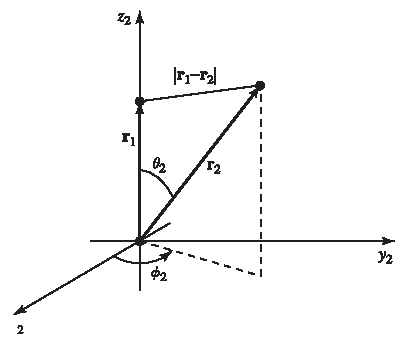
\includegraphics[height=6cm]{fig/r2_integral.pdf}
    \caption{耦合积分中的坐标选择,本图来自 Griffth 书的图 7.4}
    \label{fig:coupled_r2}
\end{figure}
注意到,这两个电子的坐标都是自由的。我们尝试\textbf{分开求解},分而治之,把 $r_1$ 看成是固定的,能否积掉 $r_2$?利用这个假设,参照图 \ref{fig:coupled_r2} 的定义,那么
\begin{align}
    r_12 = |r_1 - r_2| = \sqrt{r_1^2 + r_2^2 - 2r_1 r_2 \cos\theta_2}. 
\end{align}
先求解其中 $\theta_2$ 的积分(下面 $I_2$ 的 2 仅用来标记积分内容,无特殊含义,后面的 $I_3$ 等同理),
\begin{align}
    I_2&=\int_0^\pi \sin\theta_2 \, \frac1{r_{12}} \dd\theta_2 \\
    &=\int_0^\pi \frac{\sin\theta_2}{\sqrt{r_1^2 + r_2^2 - 2r_1 r_2 \cos\theta_2}}\dd\theta_2
\end{align}
设 $x = -\cos\theta_2$,则 $\dd x = \sin\theta_2\dd\theta_2$,代回上式,
\begin{align}
    I_2 &= \int_{-1}^1 \frac{\dd x}{\sqrt{r_1^2 + r_2^2 - 2r_1 r_2 x }}
\end{align}
利用积分公式
\begin{align}
    \int \frac{\dd x}{\sqrt{a+bx}} = \frac2b \sqrt{a+bx}
\end{align}
继续求解
\begin{align}
    I_2&= \frac{2}{2r_1r_2} \left(
        \sqrt{r_1^2 + r_2^2 + 2r_1r_2} - \sqrt{r_1^2+r_2^2 - 2r_1r_2}
    \right) \\
    &= \frac1{r_1r_2} \left(
        r_1 + r_2 - |r_1 - r_2|
    \right)\\
    &= \frac1{r_1r_2} \times \begin{cases}
        2r_2, \quad & r_1 \geqslant r_2, \\
        2r_1, \quad & r_1 < r_2,
    \end{cases} 
    = \begin{cases}
        \frac{2}{r_1}, \quad r_1 \geqslant r_2, \\
        \frac{2}{r_2}, \quad r_1 < r_2, 
    \end{cases}
    \\
    &= \frac2{\max\{r_1, r_2\}},
\end{align}
再求其余跟 $r_2$ 相关的部分
\begin{align}
    I_3{}& \int_0^\infty r_2^2 \dd r_2 \int_0^\pi \sin\theta_2 \dd\theta_2 \int_0^{2\pi}\dd\varphi_2 \frac1{r_{12}}
    \exp\left[-\frac{2\lambda}{a_0}(r_1 + r_2)\right] 
    \\
    ={}& \int_0^\infty r_2^2 \dd r_2 \exp\left[
        -\frac{2\lambda(r_1 + r_2)}{a_0}
    \right] \frac{2}{\max\{r_1, r_2\}} 
    \int_0^{2\pi} \dd\varphi_2 \\
    ={}& 4\pi \exp\left(-\frac{2\lambda r_1}{a_0}\right) 
    \int_0^{+\infty} r_2^2 \exp\!\left(-\frac{2\lambda}{a_0}r_2\right) \frac1{\max\{r_1, r_2\}} \dd r_2, 
\end{align}
其中的 max 相当于分段函数,分开积分
\begin{align}
    I_3 &= 4\pi \exp\left(
        -\frac{2\lambda r_1}{a_0}\right)
        \left[
            \int_0^{r_1} r_2^2 \exp\left(- \frac{2\lambda}{a_0}r_2\right) \frac1{r_1} + \int_{r_1}^{r_2} \exp\!\left(-\frac{2\lambda}{a_0}r_2\right) \frac1{r_2} \dd r_2
        \right]
\end{align}
利用已知积分
\begin{align}
    &\int r \ee^{-ar} \dd r= - \frac{ra + 1}{a^2} \ee^{-a r}, \\
    &\int r^2 \ee^{-ar}\dd r = - \frac{r^2a^2 + 2ra + 2}{a^3} \ee^{-ar},
\end{align}
继续求解积分,
\begin{align}
    I_3 &= 4\pi \exp\left(- \frac{2\lambda}{a_0}r_1\right) 
    \Bigg[
        \frac 1{r_1} - \frac{r_1^2 \left(\frac{2\lambda}{a_0}\right)^2 + 2 \frac{2\lambda}{a_0} r_1 + 2}{\left(\frac{2\lambda}{a_0}\right)^3} \exp\left(-\frac{2\lambda}{a_0}r_1\right) \notag\\
    &\phantom{=} + \frac{2}{\left(\frac{2\lambda}{a_0}\right)^3} + \frac{r_1 \left(\frac{2\lambda}{a_0}\right) + 1}{\left(\frac{2\lambda}{a_0}\right)^2} \exp\!\left(-\frac{2\lambda}{a_0}r_1\right)\Bigg]\\
    &=\frac{4\pi a_0^3}{8\lambda^3} \frac1{r_1} \exp\!\left(-\frac{2\lambda}{a_0}r_1\right) 
    \left[
        -\left(\frac{2\lambda}{a_0}r_1 + 2\right) \exp\!\left(-\frac{2\lambda}{a_0}r_1\right) + 2
    \right] \\
    &=\frac{\pi a_0^3}{\lambda^3} \frac1{r_1} \left[
        \exp\left(-\frac{2\lambda}{a_0}r_1\right) - \left(1+\frac{\lambda}{a_0}r_1\right) \exp\left(-\frac{4\lambda}{a_0}r_1\right)
    \right]
\end{align}
求解完了 $r_2$ 相关的部分,把这个积分代回 $r_{12}$ 的积分中去,有
\begin{align}
    &\int_0^{+\infty} r_1^2 \dd r_1 \frac{\pi a_0^3}{\lambda^3} \frac1{r_1}  
    % \notag \\ &\quad \times
    \left[
        \exp\!\left(-\frac{2\lambda}{a_0}r_1\right) - \left(1+\frac{\lambda}{a_0}r_1\right) \exp\left(-\frac{4\lambda}{a_0}r_1\right)
    \right] \notag \\
    &\quad \times \int_0^\pi \sin\theta_1 \dd\theta_1
    \int_0^{2\pi} \dd\varphi_1 \\
    =& \frac{4\pi^2 a_0^3}{\lambda^3} \int_0^{+\infty} r_1 
    \left[
        \exp\!\left(-\frac{2\lambda}{a_0} r_1\right) - \exp\!\left(-\frac{4\lambda}{a_0}r_1\right) - 
        \frac{\lambda}{a_0} r_1 \exp\!\left(-\frac{4\lambda}{a_0} r_1\right)
    \right] \dd r_1 \notag
    \\
    =& \frac58 \frac{\pi a_0^5}{\lambda^5}
\end{align}
最终有 $r_{12}^{-1}$ 部分的积分为
\begin{align}
    \bigg\langle \psi_0 \bigg| \frac1{r_{12}} \bigg| \psi_0 \bigg\rangle = \frac1{\pi^2}\left(\frac{\lambda}{a_0}\right)^6 \times \frac58 \frac{\pi a_0^5}{\lambda^5} = \frac58 \frac{\lambda}{a_0},
\end{align}
则
\begin{align}
    f(\lambda) &= \frac{\lambda^2 - 4\lambda}{ma_0}\hbar^2 + \frac{\hbar^2}{ma_0} \frac58 \frac{\lambda}{a_0} \\
    &= \frac{\hbar^2}{ma_0} \left(\lambda^2 - \frac{27}8 \lambda\right), 
\end{align}
对变分参数求偏导可得
\begin{align}
    \pdv{f(\lambda)}{\lambda} = 0 \ \Rightarrow \ \lambda = \frac{27}{16} = \num{1.6875}.
\end{align}
由于电子的相互排斥,相当于对有效核电荷起到了屏蔽效应,使得电子感受到的平均核电荷有相互吸引的部分。此时基态能量为
\begin{align}
    E_0 \approx \langle \psi_0|\hat H | \psi_0\rangle = \frac{\hbar^2}{ma_0} \left(\lambda^2 - \frac{27}8 \lambda\right) \approx \num{-2.848} \frac{\hbar^2}{ma_0} \geqslant E_0 = \num{-2.904} \frac{\hbar^2}{ma_0}. 
\end{align}
由参数 $\lambda$ 便可以给出氦原子基态能量的近似值,我们看到确实变分能量高于真实能量。

% 2022-11-07 15:03:15 Wenbin FAN @FDU
变分法不能保证,构造出的试探波函数空间一定涵盖真实的波函数,如果能够涵盖基态波函数,如谐振子模型,但绝大多数体系是不可能的,如氦原子是最简单的一个做不到的例子。虽然我们做不到精确,但是我们可以不断逼近。

有没有办法可以更好地逼近?回头来审视最初的设定,如果两个例子感受到的有效电荷不一样,是否能更精确地求解?
\homework{\textbf{8.3}  请用下述波函数作为尝试波函数,
\begin{align}
    \Phi_0 = N \left(
        \ee^{-\lambda_1 r_1/a_0} \ee^{-\lambda_1 r_2} + 
        \ee^{-\lambda_2 r_1/a_0} \ee^{-\lambda_2 r_2}
    \right),
\end{align}
变分积分为 $f(\lambda_1, \lambda_2) = \langle \Phi_0 | \hat H | \Phi_0 \rangle$,对于 BO 近似下的氦原子电子基态能量进行变分,能量约为 $\num{-2.88}\frac{\hbar^2}{ma_0}$,参考 Eckart, C. (1930). The theory and calculation of screening constants. \emph{Physical Review}, \emph{36}(5), 878. DOI: 10.1103/PhysRev.36.878 。
}

%2022-11-07 15:09:03 Wenbin FAN @FDU
能否得到激发态能量?也可以的,通过正交的方式得到,具体拓展下节课线下再讲。
% 2022-11-14 07:59:19  Wenbin Fan @FDU
\section{复习}
\courseTime{第9次课,第11周,Nov04}
\chat{%
今天人好少(只有 13 位同学,不包括助教等),被隔离了吗?

% 2022-11-14 08:03:33  Wenbin Fan @FDU
上周第十周,我们介绍了变分法。它本质上是为了求解定态薛定谔方程,
\begin{align}
    \hat H \psi = E \psi,
\end{align}
原理上是说,平均值可以写成
\begin{align}
    \hat F = \frac{\langle \psi | \hat F | \psi \rangle}{\langle \psi | \psi \rangle},
\end{align}
哈密顿算符是很复杂的,有动能和势能,
\begin{align}
    \hat H = \hat T + \hat V = -\frac{\hbar^2}{2} \sum_i \frac{1}{m_i}\hat \nabla_i^2
    + \sum_i V_{\mathrm{ext}}(\vec r_i) 
    +\sum_{i<j}V_{\mathrm{int}}(\vec r_i, \vec r_j),
\end{align}
% 2022-11-14 08:06:44  Wenbin Fan @FDU
以氦原子为例,哈密顿算符为
\begin{align}
    \hat H = 
    -\frac{\hbar^2}{2m_{\mathrm{He}}} \hat \nabla_1^2
    -\frac{\hbar^2}{2m_{\mathrm{e}}} \left(\hat \nabla_2^2 + \hat \nabla_3^2\right)
    - \frac{2e^2}{|\vec r_2 - \vec r_1|} - \frac{2e^2}{|\vec r_3 - \vec r_1|}
    + \frac{e^2}{|\vec r_2 - \vec r_3|}
\end{align}
如果把原子核、电子都当作粒子本身,外势就不存在了。未来几周会讲全同粒子、自旋。氦原子的波函数 $\psi(\vec r_1, \vec r_2, \vec r_3)$ 是 $3\times3=9$ 维的。
}

变分原理告诉我们,能量的期望值大于基态能量,对于尝试波函数 $\psi_0$
\begin{align}
    \frac{\langle \psi_0 | \hat H | \psi_0 \rangle}{\langle \psi_0 | \psi_0 \rangle} = \bar E_0 \geqslant E_0
\end{align}
如果变分空间涵盖真实波函数,则一定可求解得到基态能量。若 $\psi_0$ 归一,则有
\begin{align}
    \langle \psi_0 | \hat H | \psi_0 \rangle \geqslant E_0. 
\end{align}

\chat{%
并不知道如何探索波函数空间,但我们可以引入超参数构成的波函数空间。
}设定尝试波函数 $\psi_0(\vec r_1, \vec r_2, \cdots, \vec r_n; c_1, c_2, \cdots, c_n)$,
%2022-11-14 08:12:34  Wenbin Fan @FDU
方法是近似的,原理是精确的。对参数 $\{c_1, c_2, \cdots, c_n\}$ 求偏微分,满足 $\left\{\pdv{\bar E}{c_i}=0\right\}$。

\chat{%
上节课讲过的第一个例子是谐振子,我们知道真实的基态波函数是高斯展宽的形式,
\begin{align}
    \Phi_0 = N \exp\!\left(-\frac12 \frac{m\omega}{\hbar}x^2\right),
\end{align}
为了验证这个解的正确性,设定尝试波函数
\begin{align}
    \psi_0 = N \ee^{-ax^2} \ \Rightarrow \bar E(a). 
\end{align}
为什么 $\psi_0 = N \ee^{ax^2}$ 不能当作尝试波函数?因为尝试波函数必须与哈密顿量有共同的边界条件,这个尝试波函数得到的并非是束缚态,所以得到的「基态」能量是错的。

% 2022-11-14 08:17:52  Wenbin Fan @FDU
第二个例子是氦原子。它是个 9 维的系统,对它做的第一件事是 BO 近似,分离原子核和电子的运动。
把原子核当成独立的外势,
原子核对电子的吸引看作是系统依赖的外势。
氢分子和氦原子都是两个电子,如果要构建哈密顿量,动能算符是一样的,库伦排斥算符也是一样的,区别在于势能不同。更普适地,对于 $N$ 电子的系统,动能算符和库伦排斥算符都是一样的,只是势能不同。五彩斑斓的化学世界正是来自于这个势能。
}

求解氦原子的第一步是把完整的哈密顿量近似成原子核的独立运动和电子的独立运动,原子核和电子的相互作用被看作成外势,这种近似称作 Born--Oppenheimer 近似。设尝试波函数
\begin{align}
    \psi_0(r_1, r_2; \lambda) = \frac{\lambda^2}{\pi a_0^3} 
    \ee^{-\frac{\lambda}{a_0}(r_1 + r_2)}, 
\end{align}
\chat{%
我们这么设,是因为确实不知道波函数是什么形式。这个形式来自于类氢离子的波函数,将核电荷数设定为变分参数,我们认为电子感受到的力并不是单纯来自原子核的吸引,而是有一部分电子的排斥,吸引和排斥的平均效应。
}
由公式变分原理公式,得到 $\lambda = \num{1.6875}$,$E-\lambda = 0.3125$ 个排斥能,变分能量 $\bar E_{\mathrm{min}} = -\num{2.848} \frac{\hbar^2}{ma_0^2}$,真实能量为 $E_0 = -2.904 \frac{\hbar^2}{ma_0^2}$,误差 1.93\%。
\chat{%
误差有点大,能否有更好的近似?

从误差可知,我们设定的尝试波函数还不够包含真实的氦原子波函数空间,人们找了很多合适的尝试波函数。下面介绍一个非常直观的改进。
% 2022-11-14 08:27:46  Wenbin Fan @FDU
势能与两电子的距离有关 $\frac{e^2}{r_{23}}$,当两个电子越靠近,出现的概率越小,这里暂不考虑是交换还是相关贡献,只考虑库伦相互作用。也就是说,波函数不仅与两个电子独立的概率分布有关,也与两电子的距离相关。
}

波函数仅仅表示成 $r_1, r_2$ 的形式不够,后来 Egil Hylleraas 提出了有明确物理意义的超参数,
\begin{align}
    \psi_0 = N \left[
        \ee^{-\frac{\lambda}{a_0}(r_1+r_2)}(1 + b\, r\!_{12})
    \right],
\end{align}
% 波函数与两个电子的距离有关。
此时变分参数为 $\{\lambda, b\}$,对二者分别求偏微分得到 $\lambda = 1.849$、$b = 0.364$,有效屏蔽更小了,有一部分电子-电子相互作用,不再需要粗糙的平均场近似给出。变分能量 $\bar E_{\mathrm{min}}(\lambda, b) = \SI{-78.4}{\electronvolt}$,误差为 $0.4\%$。

进一步考虑这种尝试波函数,
\begin{align}
    \psi_0 = N \left[ 
        \ee^{-\frac{\lambda}{a_0}(r_1 + r_2)}
    \sum_{ijk} c_{ijk} (r_1 + r_2)^i (r_1 - r_2)^j r_{12}^k
    \right],
\end{align}
变分超参数为 $\{\lambda, c_{ijk}\}$,得到近似值为 $E_0 = \num{-2.903724375} \frac{\hbar^2}{ma_0^2}$,实验值为 $E_0 = \num{-2.903724376} \frac{\hbar^2}{ma_0^2}$,误差小于 $\SI{2.7e-8}{\electronvolt}$。
% 2022-11-14 08:36:17  Wenbin Fan @FDU
\chat{%
如果更好地构造尝试波函数、变分空间,可以得到更精确的解。我们不能搜索整个大海,只能构造子空间去搜索,所有的困难都在于如何让这个子空间包含精确解。

有没有更系统的方法?
}

\section{线性变分法}
\chat{%
线性变分法是说,我不知道怎么构造这个复杂的函数空间。比如氦原子,从构造波函数开始就很困难,我们需要知道大致的解析解、假设参数、设定变分参数的物理意义,并创造性地构造尝试波函数。我们很自然地考虑,有没有另外的方式构造函数空间?
% 搜索变得很困难。

线性厄米算符的本征函数构成完备集,所有具有相同边界条件的品优波函数,都可以由这个完备集严格展开。
}

% 意味着,我们可以把波函数写成任意一个具有相同本征函数的线性展开。
我们任选一组满足边界条件的函数 $f_i$,用来展开待求波函数,这组函数没有要求是本征解或者满足正交归一的条件。
% 那么将【】
% 2022-11-14 08:39:55  Wenbin Fan @FDU
原则上,展开后是无穷多项的,
\begin{align}
    \psi_0 = c_1 f_1 + c_2 f_2 + \cdots + c_n f_n = \sum_{i=1}^n c_i f_i,
\end{align}
如果 $\{f_i\}$ 就是 $\hat H$ 的本征解,变分可得 $\{c_1 = 1, c_2=0, \cdots, c_n =0\}$。如果 $\{f_i\}$ 不是 $\hat H$ 的本征解,但是 $\{f_i\}$ 为正交归一的完备集,那么可以解出
\begin{align}
    \langle f_i | \psi_0 \rangle = \sum_j \langle f_i | f_j \rangle = \sum_j c_j \delta_{ij} = c_i.
\end{align}

(1) 做归一化判断,
\begin{align}
    \langle \psi_0 | \psi_0 \rangle = \sum_{i}\sum_j c_i^* c_j \langle f_i | f_j \rangle = \sum_i \sum_j c_i^* c_j S_{ij}, 
\end{align}
其中
\begin{align}
    S_{ij} \equiv \langle f_i | f_j \rangle = \int f_i^* f_j \dd\tau, 
\end{align}
这里 $S_{ij}$ 和 $\delta_{ij}$ 是不同的,因为没有假设 $\{f_i\}$ 之间正交。

\chat{%
看起来人变少了。同学们还能自由选课吗,还是说逃课了。这对任课教师来说没有任何影响,只要同学们真正学到知识就好。
上学期期末考试有点难,卷面成绩很少过 60 的,大都靠平时成绩提分,注意平时作业。
}

\courseTime{2 of 4, week 09, Nov14}
% 2022-11-14 08:55:42  Wenbin Fan @FDU
(2) 重叠积分
\begin{align}
    \langle \psi_0 | \hat H | \psi_0 \rangle = 
    \sum_i \sum_j c_j^* c_j \langle f_i | \hat H | f_i \rangle = \sum_i \sum_j c_i^* c_j H_{ij},
\end{align}
其中
\begin{align}
    H_{ij} \equiv \langle f_i | \hat H | f_j \rangle = \int f_i^* \hat H f_j \dd\tau. 
\end{align}
因此,平均能量,
\begin{align}
    \bar E(c_1, c_2, \cdots, c_n) = \frac{\langle \psi_0 | \hat H | \psi_0 \rangle}{\langle \psi_0 | \psi_0 \rangle} = \frac{\sum_i \sum_j c_i^* c_j H_{ij}}{\sum_i \sum_j c_i^* c_j S_{ij}},
\end{align}
把它写成一行
\begin{align}
    \bar E \sum_i \sum_j c_i^* c_j S_{ij} = \sum_i \sum_j c_i^* c_j H_{ij}. 
\end{align}

为了展开变分 $\left\{\frac{\partial \bar E}{\partial c_i} = 0\right\}$,对等式两边求偏导
\begin{align}
    \pdv{c_k} \left[
        \bar E \sum_i \sum_j c_i^* c_j S_{ij}
        \right]
    &= \pdv{c_k} \sum_j \sum_j c_i^* c_j H_{ij} \notag\\
    \pdv{\bar E}{c_k} \sum_i \sum_j c_i^* c_j S_{ij} + 
    \bar E
    \sum_i \sum_j \left(\pdv{c_k}c_i^* c_j\right) S_{ij} &= 
    \sum_i \sum_j \left(\pdv{c_k}c_i^* c_j\right) H_{ij},
    \label{eq:perb_vari_dedci_1}
\end{align}
% 2022-11-14 08:59:59  Wenbin Fan @FDU
其中,关键的地方在于
\begin{align}
    \pdv{c_k} c_i^* c_j = \left(\pdv{c_k}c_i^*\right) c_j + c_i^* \left(\pdv{c_k} c_j\right),
\end{align}
因为各参数之间没有关系,
% 【什么无关,返回去看平均能量定义】,
所以
\begin{align}
    \pdv{c_i}{c_k} = \pdv{c_i^*}{c_k^*} = 0, \quad i\neq k. 
\end{align}
\chat{%
大家学过复变函数吗?这里要用到复变函数里的关键结论。
}
\suppInfo{复变函数的连续性——柯西定理}{
柯西连续性,有
\begin{align}
    \begin{cases}
        \pdv{c_i}{c_i} = 1, \\ \pdv{c_i^*}{c_i} = 0, 
    \end{cases}\quad \text{其中}
    \begin{cases}
        c_i = x+y \ii, \\
        c_i^* = x - y \ii, 
    \end{cases}
\end{align}
简单证明之。复变函数的普遍形式 $f(z) = \mu(x,y) + \ii\,\nu(x,y)$,并且设
\begin{align}
    & c_i \quad \mu = x, \nu = y,\\
    & c_i^* \quad \mu = x, \nu = -y. 
\end{align}
求函数 $f(z)$ 的偏导,即函数随自变量的响应,
\begin{align}
    f'(z) = \lim_{\Delta z\rightarrow 0} \frac{f(z+\Delta z) - f(z)}{\Delta z} = ?, \quad \Delta z = \Delta x + \ii \Delta y. 
\end{align}

当 $\Delta z$ 是沿着 $x$ 轴方向逼近 $z$,则 $\Delta z = \Delta x$,$\Delta y = 0$,
\begin{align}
    f'(z) &= \lim_{\Delta x\rightarrow0} 
    \left[
        \frac{\mu(x+\Delta x, y) - \mu(x, y)}{\Delta x}
        + \ii \frac{\nu(x+\Delta x, y) - \nu(x, y)}{\Delta x}
    \right] \notag\\
    &= \pdv{\mu}{x} + \ii\pdv{\nu}{x},
\end{align}
同理,当 $\Delta z$ 沿着 $y$ 轴逼近 $z$,则 $\Delta z = \ii\Delta y$、$\Delta x =0$,
\begin{align}
    f'(z) = \pdv{\nu}{y} - \ii\pdv{\mu}{y}. 
\end{align}
为了使得 $f(z)$ 处处可导,则
\begin{align}
    f'(z) = \pdv{\mu}{x} + \ii \pdv{\nu}{x} = \pdv{\nu}{y} - \ii\pdv{\mu}{y},
\end{align}
推知
\begin{align}
    \begin{cases}
        \displaystyle
        \pdv{\mu}{x} = \pdv{\nu}{y}, \\
        \noalign{\vskip9pt}
        \displaystyle
        \pdv{\nu}{x} = -\pdv{\mu}{y},
    \end{cases}
\end{align}
称作\boldtext{柯西--黎曼方程} Cauchy--Riemann。复空间的函数连续性要更严格。

对本例来说,前设 $c_i$ 满足 CR 方程,但 $c_i^*$ 不满足。
因此我们得到了复变函数中的结论,如果一个函数是连续可导的,那么它的共轭一定不是连续可导的。

% 2022-11-14 09:13:06  Wenbin Fan @FDU
在工程中,为了保证函数可导数,比如可采用 Wirtinger 导数定义,那么
\begin{align}
    \pdv{z} = \frac12 \left(\pdv{x} - \ii \pdv{y}\right), 
    \quad
    \pdv{z^*} = \frac12\left(\pdv{x}+\ii \pdv{y}\right),
\end{align}
证明了
\begin{align}
    \pdv{z}{z} = 1, \quad \pdv{z^*}{z} = 0,
\end{align}
可用 $\delta$ 记号写成
\begin{align}
    \pdv{c_i}{c_k} = \delta_{ik} = \begin{cases}
        1, \quad &i=k,\\
        0, \quad &i\neq k. 
    \end{cases}
\end{align}
% 为了保证共轭与自身无关,工程上的应用。
}

按照复变函数的偏导,只留下第 $k$ 项,
\begin{alignat}{2}
    &\pdv{c_k} \sum_i \sum_j c_i^* c_j S_{ij} = \sum_i \sum_j c_i^* \pdv{c_i}{c_k} S_{ij} &&= \sum_i c_i^* S_{ik}, \\
    &\pdv{c_k} \sum_j \sum_j c_i^* c_j H_{ij} &&= \sum_i c_i^* H_{ik}, 
\end{alignat}
这里是对 $c_k$ 求偏导,留下了 $c_k^*$,等价地,也可对 $c_k^*$ 求偏导留下 $c_k$。
% % 2022-11-14 09:16:02  Wenbin Fan @FDU
% 同理
% \begin{align}
%     1
% \end{align}
% 这之前的 S 写成了 delta,正确的是 S
% 重要:前面某处漏了 \bar E,在某个求和之前
继续求 \eqref{eq:perb_vari_dedci_1},因为其中 $\pdv{\bar E}{c_k} =0$,只剩下了另外两项,有
\begin{align}
    \bar E \sum_i c_i^* S_{ik} = \sum_i c_i^* H_{ik},
\end{align}
% 2022-11-14 09:19:31  Wenbin Fan @FDU
% 新一页
两边都是对 $i$ 求和,重新规整得到
\begin{align}
    \sum_i  [c_i^* \left(\bar E S_{ik} - H_{ik}\right)] = 0, \quad k = 1, \cdots, n. 
\end{align}
如果我们重复一遍上述偏导的流程,但是对 $c_k^*$ 求偏导,那么得到
\begin{align}
    \sum_i  [c_i \left(\bar E S_{ik} - H_{ik}\right)] = 0, \quad k = 1, \cdots, n. 
\end{align}
我们得到了线性方程组。为了让这 $n$ 个方程有非平凡解,其久期行列式为 0,
\begin{align}
    \left|
        \begin{matrix}
            \bar E S_{11} - H_{11} & \bar E S_{12} - H_{12} & \cdots & \bar E S_{1n} - H_{1n} \\
            \bar E S_{21} - H_{21} & \bar E S_{22} - H_{22} & \cdots & \bar E S_{2n} - H_{2n} \\
            \vdots & \vdots & \ddots & \vdots \\
            \bar E S_{n1} - H_{n1} & \bar E S_{n2} - H_{n2} & \cdots & \bar E S_{nn} - H_{nn} \\
        \end{matrix}
    \right| = 0,
\end{align}
可以解出 $N$ 个解,
\begin{align}
    \bar E_0 \leqslant \bar E_1 \leqslant \bar E_2 \leqslant \cdots \leqslant \bar E_n. 
\end{align}
\chat{%
上周没讲激发态变分,实际上激发态的变分跟基态变分是一样的,只需要激发态变分函数和基态是正交的,由此确定变分空间,可以证明说,这样的变分空间给出的激发态最低能量是要大于激发态的能量。}
这里求解的 $E_0$ 大于真实的基态能量,$E_1$ 大于真实的第一激发态能量
\begin{align}
    \bar E_0 \geqslant E_0, \quad \bar E_1 \geqslant E_1, \quad \cdots, \quad \bar E_n \geqslant E_n. 
\end{align}
\chat{%
求解激发态能量的困难在于,基态不准确的话,激发态也会更加不准。激发态的电子关联效应会更强,更难处理。从数学上来说,第一步的变分法(基态)没做好,后面的步骤(激发态)会偏离更多,称作误差累积效应。
}

% 2022-11-14 09:23:40  Wenbin Fan @FDU
\homework{\textbf{9.1} 求值
\begin{align}
    \left|\ \begin{matrix}
        2 & \phantom{-}5 & \phantom{-}1 & \phantom{-}3 \\ 
        8 & \phantom{-}0 & \phantom{-}4 & -1 \\ 
        6 & \phantom{-}6 & \phantom{-}6 & \phantom{-}1 \\ 
        5 & -2 & -2 & \phantom{-}2
    \end{matrix}\ 
    \right|
\end{align}
}

\chat{%
变分讲完了,没有证明激发态变分法,同学们可参考物化课的讲解,跟这里的内容相互印证,以便更好理解。

同学们觉得难吗?我们尽量一步步展开求解问题,没有跳步,这是教师的初衷。只要是一步步跟下来,肯定能学会,甚至能举一反三提出问题。如果是 PPT 填鸭教育,同学们可能学不到什么,最终「不知所然」。本课是配套强基计划教改,当时写过大纲,如果按照这个推导速度,一半内容都讲不到,后续的 Hartree--Fock、耦合簇 coupled cluster、微扰等实用方法都讲不到。本课的内容介于量子力学和高等量子力学之间,并不完全属于高等量子力学,因为高量中是用二次量子话的语言描述。

% 2022-11-14 09:28:34  Wenbin Fan @FDU
微扰理论跟变分法类似,都是不断逼近精确解的过程。微扰理论的难点在于如何更有效地构建变分空间,一旦构造成功,求解相对容易。这节课讲到了线性变分,提供了一条构造变分空间的策略。出发点是好的,但求解难度甚大。

% 2022-11-14 09:29:02  Wenbin Fan @FDU
对于复杂体系而言,线性厄米算符构成的完备集是无穷大的,我们是做了截断。真实体系中,高斯型基组通常是几千个,平面波基组会上万个,这里截断会引入基组不完备的误差。计算标度 scaling 与基组的数量 $N$ 呈指数关系,通常是 3---4 次方甚至更高。以相对小的三次方为例,假设 10 个水 10 秒算完,那么很容易算出来 20 个水是 80 秒算完,100 个水是 \num{10000} 秒算完,1000 个水将需要将耗时 $\SI{1e7}{\second} = \SI{116}{\day}$,\num{10000} 个水将耗时 $\SI{1e10}{\second} = \SI{317}{year}$。这种指数增长阻碍了大体系的求解,被形象地称作「指数墙」,一种解决途径是利用各种近似,也有课题组开发线性标度的计算软件。
}

\chapter{微扰}
\chat{%
当我们找不到较好的变分空间时,应该怎么做?
}

% 2022-11-14 09:31:19  Wenbin Fan @FDU
假设定态薛定谔方程 $\hat H \psi_n = E_n \psi_n$ 不能精确求解,又假设 $\hat H$ 与 $\hat H_0$ 只有微小差别,且 $\hat H_0$ 相对容易求解
\begin{align}
    \hat H_0 \psi_n^{(0)} = E_n^{(0)} \psi_n^{(0)}. 
\end{align}
\chat{%
高数中讲级数展开,前提是在定义域、收敛域内展开。在我们的假设下,整体的哈密顿量 $\hat H$ 分成了两部分。
}
% 微扰展开【】,是能求解的
% \begin{align}
%     \hat H_0 []
% \end{align}

例1,一维非谐振子,在光谱研究中常常会考虑超越谐振近似的非谐效应,
\begin{align}
    \hat H = -\frac{\hbar^2}{2m} \pdv[2]{x} + \frac12 kx^2 + cx^3 + dx^4,
\end{align}
其中的谐振子部分
\begin{align}
    \hat H_0 = -\frac{\hbar^2}{2m} \pdv[2]{x} + \frac12 kx^2, 
\end{align}
是可以求出精确解的。若 $c,d$ 足够小,$\hat H' = cx^3 + dx^4$ 可看作对谐振子哈密顿量的微小扰动。称 $\hat H_0$ 为未微扰体系、$\hat H$ 为微扰体系。

由此可构造微扰途径,从未微扰到微扰,
\begin{align}
    \hat H = \hat H_0 + \lambda \hat H', \quad \lambda\in[0,1]. 
\end{align}
% 这个 approach 在后面用到了吗?没用到的话,可以忽略 % 2022-11-15 11:50:53 Wenbin FAN @FDU
先考虑没有能级简并的情况。如果能级有简并,可能会出现奇点。

\courseTime{3 of 4, w09, Nov 14}
\section{非简并的微扰理论}
把哈密顿量拆成两部分,
\begin{align}
    (\hat H_0 + \lambda \hat H') \psi_n = E_n \psi_n, 
    \label{eq:perb_bb_1}
\end{align}
其中 $\psi_n = \psi_n(\tau, \lambda)$,$E_n = E_n(\lambda)$,$\tau$ 表示全体坐标。 
% % 2022-11-14 13:33:13  Wenbin Fan @FDU
% 老师到
% % 2022-11-14 13:34:51  Wenbin Fan @FDU
% 继续早上的讲。早上讲了线性变分,我们继续讲微扰。微扰理论中最简单的是非简并理论。
\chat{%
什么样的微扰才算足够小?这是一个开放式的、case-by-case 的问题。
一旦做了这样的分解,波函数和能量自然就是线性微扰参数 $\lambda$ 的函数。
}
对波函数和能量做幂级数展开,
\begin{align}
    &\psi_n = \psi_n |_{\lambda = 0} + \pdv{\psi_n}{\lambda}\Big|_{\lambda = 0}\lambda + \pdv[2]{\psi_n}{\lambda}\Big|_{\lambda = 0} \frac{\lambda^2}{2!} + \cdots, 
    \label{eq:perb_bb_2} %% bb -> blackboard
    \\
    &E_n = E_n |_{\lambda = 0} + \pdv{E_n}{\lambda}\Big|_{\lambda = 0}\lambda + \pdv[2]{E_n}{\lambda}\Big|_{\lambda = 0} \frac{\lambda^2}{2!} + \cdots. 
    \label{eq:perb_bb_3}
\end{align}
我们稍微讨论一下。当 $\lambda = 0$ 时,$(\psi_n, E_n) \rightarrow (\psi_n^{(0)}, E_n^{(0)})$ 未微扰,
\begin{align}
    \psi_n |_{\lambda=0} = \psi_n^{(0)}, \quad E_n|_{\lambda=0} = E_n^{(0)}. 
\end{align}
再定义 $k$ 阶微扰,
\begin{align}
    \psi_n^{(k)} = \frac1{k!} \pdv[k]{\psi}{\lambda},
\end{align}
则波函数、能量可以写成
\begin{align}
    &\psi_n = \psi_n^{(0)} + \psi_n^{(1)}\lambda + \psi_n^{(2)} \lambda^2 + \cdots, \label{eq:perb_bb_4}\\
    &E_n = E_n^{(0)} + E_n^{(1)} \lambda + E_n^{(2)}\lambda^2 + \cdots, \label{eq:perb_bb_5}
\end{align}
零级、一级、二级等高阶项。
\chat{%
其实 \eqref{eq:perb_bb_4}、\eqref{eq:perb_bb_5} 是 \eqref{eq:perb_bb_2}、\eqref{eq:perb_bb_3} 重写的。
}
把 \eqref{eq:perb_bb_4} 和 \eqref{eq:perb_bb_5} 代回到 \eqref{eq:perb_bb_1} 中,有
\begin{multline}
    (\hat H_0 + \lambda \hat H') \left(
        \psi_n^{(0)} + \psi_n^{(1)}\lambda + \psi_n^{2} \lambda^2 + \cdots
    \right) \\= 
    \left(
        E_n^{(0)} + E_n^{(1)} \lambda + E_n^{(2)}\lambda^2 + \cdots
    \right)
    \left(
        \psi_n^{(0)} + \psi_n^{(1)}\lambda + \psi_n^{(2)} \lambda^2 + \cdots
    \right)
\end{multline}
将 $\lambda$ 相同幂级数的项归并,重写成
\begin{multline}
    \hat H_0 + \lambda \left(
        \hat H' \psi_n^{(0)} + \hat H_0 \psi_n^{(1)}
    \right) + \lambda^2 \left(
        \hat H' \psi_n^{(1)} + \hat H_0 \psi_n^{(2)}
    \right) \cdots \\ = 
    E_n^{(0)} \psi_n^{(0)} + \lambda \left(
        E_n^{(1)} \psi_n^{(0)} + E_n^{(0)} \psi_n^{(1)} + 
    \right) 
    \\+ \lambda^2 \left(
        E_n^{(0)} \psi_n^{(2)} +E_n^{(1)} \psi_n^{(1)} + E_n^{(2)} \psi_n^{(0)}
    \right) + \cdots
\end{multline}
各项对应相等。对于 $\lambda^0$,
\begin{align}
    \hat H_0 \psi_n^{(0)} = E_n^{(0)} \psi_n^{(0)},
\end{align}
对于 $\lambda^1$,
\begin{align}
    \hat H' \psi_n^{(0)} + \hat H_0 \psi_n^{(1)} &= E_n^{(1)} \psi_n^{(0)} + E_n^{(0)} \psi_n^{(0)} \\
    (\hat H_0 - E_n^{(1)})\psi_n^{(1)}&= - (\hat H' - E_n^{(1)}) \psi_n^{(0)},
\end{align}
左边是一级波函数。因为 $\hat H_0$ 是线性厄米算符,$\{\psi_n^{(0)}\}$ 正交归一,构成完备集,
\begin{align}
    \psi_n^{(0)} = \sum_j a_j \psi_j^{(0)}
\end{align}
用零级波函数展开一级波函数,
\begin{align}
    \sum_j a_j (\hat H_0 - E_n^{(0)}) \psi_j^{(0)} &= - (\hat H' - E_n^{(1)}) \psi_n^{(0)}\\
    \sum_j a_j (E_j^{(0)} - E_n^{0)}) \psi_j^{(0)} &= - (\hat H' - E_n^{(1)}) \psi_n^{(0)},
\end{align}
左乘 $\langle \psi_m^{(0)}|$,
\begin{align}
    \sum_j a_j (E_j^{(0)} - E_n^{(0)}) 
    \underbrace{\langle \psi_m^{(0)} | \psi_j^{(0)} \rangle}_{\delta_{mj}}
    &= E_n^{(1)} 
    \underbrace{\langle \psi_m^{(0)} | \psi_n^{(0)} \rangle}_{\delta_{mn}}
    - 
    \underbrace{\langle \psi_m^{(0)} | \hat H' | \psi_n^{(0)} \rangle}_{H'_{mn}} \\
    a_m (E_m^{(0)} - E_n^{(0)}) &= E_n^{(1)} \delta_{mn} - H'_{mn}, 
\end{align}
其中 $n$ 是我们希望求得的量子态。
\chat{如果是基态则 $n=0$。记得我们是对 $n$ 做展开的。}
% 【前面方程的 (1)(0) 有修改】
% 已改 % 2022-11-15 13:07:54 Wenbin FAN @FDU

讨论 (1) 当 $m=n$ 时,
\begin{align}
    E_n^{(1)} = H_{nn}' = \langle \psi_n^{(0)} | \hat H' | \psi_n^{(0)} \rangle
\end{align}
\chat{一级微扰的校正能量等于微扰哈密顿矩阵的对角元。}
能量逐级累加,更高阶的能量在后面会讲到,
\begin{align}
    E_n = E_n^{(0)} + E_n^{(1)} \lambda + E_n^{(2)}\lambda ^2 + \cdots.
\end{align}
当 $\lambda = 1$ 时,即微扰完全存在时,
% 【没拍……】【录像滚屏,凑合看吧】
\begin{align}
    E_n = E_n^{(0)} + E_n^{(1)} + E_n^{(2)} + \cdots, 
\end{align}
其中 $E_n^{(1)}$ 为体系能量的一级校正值,体系能量近似为
\begin{align}
    E_n \approx E_n^{(0)} + E_n^{(1)} = E_n^{(0)} + \langle \psi_n^{(0)} | \hat H ' | \psi_n^{(0)} \rangle. 
\end{align}

% 2022-11-14 13:55:53  Wenbin Fan @FDU
(2) 当 $m \neq n$ 时,
\begin{align}
    a_m (E_m^{(0)} - E_n^{(0)}) = - H'_{mn},\ \Rightarrow \ a_m = \frac{H'_{mn}}{E_n^{(0)} - E_m^{(0)}}, 
\end{align}
分子相当于基态减去激发态的能量。
% 有些忘记微扰法的整体思路了。这样板书推导定理,容易陷在局部,对整体缺少把握。应该多做题就好了
未微扰的一级波函数
\begin{align}
    \psi_n^{(1)} = \sum_{j\neq n} a_j \psi_j^{(0)} = \sum_{j\neq n} \frac{H'_{mn}}{E_n^{(0)} - E_m^{(0)}}\psi_j^{(0)}. 
\end{align}
利用 \eqref{eq:perb_bb_4},当 $\lambda = 1$,
\begin{align}
    \psi_n \approx \psi_n^{(0)} + \sum_{m\neq n} \frac{H'_{mn}}{E_n^{(0)} - E_m^{(0)}}\psi_j^{(0)}. 
\end{align}
% 当 $\lambda = 1$,
% \begin{align}
%     \psi_n \approx 
% \end{align}

% subsection? 
现考虑二级校正能量,对于 $\lambda^2$ 有
\begin{align}
    \hat H' \psi_n^{(1)} + \hat H_0 \psi_n^{(2)} &= E_n^{(0)} \psi_n^{(2)} +E_n^{(1)} \psi_n^{(1)} + E_n^{(2)} \\
    (\hat H_0 - E_n^{(0)}) \psi_n^{(2)} &= E_n^{(2)} \psi_n^{(0)} + (E_n^{(1)} - \hat H') \psi_n^{(1)}, 
\end{align}
展开 LHS 波函数的二级校正,
\begin{align}
    \psi_n^{(2)} = \sum_j b_j \psi_j^{(0)},
\end{align}
代回去有
\begin{align}
    \sum_j b_j (\hat H_0 - E_n^{(0)}) \psi_j^{(2)} = E_n^{(2)} \psi_n^{(0)} + (E_n^{(1)} - \hat H') \psi_n^{(1)},
\end{align}
左乘 $\langle \psi_m^{(0)}|$ 并积分
\begin{align}
    \sum_j b_j (E_j^{(0)} - E_n^{(0)}) \delta_{mj} &= E_n^{(2)} \delta_{mn} + E_n^{(1)} \langle \psi_m^{(0)} | \psi_n^{(1)} \rangle - \langle \psi_m | \hat H' | \psi_n^{(1)} \rangle \notag \\
    b_m (E_j^{(0)} - E_n^{(0)}) &= \cdots
\end{align}
只考虑 $m=n$ 的情况,
\begin{align}
    0 = E_n^{(2)}  + E_n^{(1)} \langle \psi_n^{(0)} | \psi_n^{(1)} \rangle - \langle \psi_n | \hat H' | \psi_n^{(1)} \rangle
    \label{eq:perb_lambdaSquared_meqn_1}
\end{align}
由一级微扰波函数可知三级微扰能量,更普适的定理是
\begin{align}
    \psi_n^{(k)} \rightarrow E_n^{(2k+1)}. 
\end{align}
% 2022-11-14 14:07:31  Wenbin Fan @FDU
继续求解 $m=n$ 的情况,
\begin{align}
    \langle \psi_n^{(0)} | \psi_n^{(1)} \rangle
    & = \langle \psi_n^{(0)} | \sum_{m\neq n}\frac{H'_{mn}}{E_n^{(0)} - E_m^{(0)}} \psi_n^{(1)} \rangle \\
    & = \sum_{j\neq n}\frac{H'_{mn}}{E_n^{(0)} - E_m^{(0)}} \langle \psi_m^{(0)} | \psi_j^{(0)} \rangle, 
\end{align}
其中 $\langle \psi_m^{(0)} | \psi_j^{(0)} \rangle = \delta_{mj}$。
% 2022-11-14 14:09:19  Wenbin Fan @FDU
从根本来说,二级微扰波函数能量就等于 \eqref{eq:perb_lambdaSquared_meqn_1} 最后一项。
% 【只考虑 m eq n 后面的式子的最后一项】。

当 $m=n$ 时,$\langle \psi_n^{(0)} | \psi_n^{(1)} \rangle = 0$,二级能量
\begin{align}
    E_n^{(2)} &= \langle \psi_n^{(0)} | \hat H' | \psi_n^{(1)} \rangle \\
    &= \langle \psi_n^{(0)} | \hat H' | \sum_{j\neq n}\frac{H'_{jn}}{E_n^{(0)} - E_j^{(0)}} \psi_j^{(0)} \rangle \\
    &= \sum_{j\neq n}\frac{H'_{jn}}{E_n^{(0)} - E_m^{(0)}}
    \underbrace{\langle \psi_n^{(0)} | \hat H' | \psi_j^{(0)} \rangle}_{H'_{nj}} \\
    &= \sum_{j\neq n}\frac{|H'_{jn}|^2}{E_n^{(0)} - E_m^{(0)}},
\end{align}
% 其中 $\langle \psi_n^{(0)} | \hat H' | \psi_j^{(0)} \rangle$ 记作 $H_{ij}'$。
由此可知,
\begin{align}
    E_n &\approx E_n^{(0)} + E_n^{(1)} + E_n^{(2)} \\
    &= E_n^{(0)} + H'_{nn} + \sum_{j\neq n} \sum_{j\neq n}\frac{|H'_{jn}|^2}{E_n^{(0)} - E_m^{(0)}}. 
\end{align}

\section{氦原子的微扰求解}
\courseTime{4th 第9次课}
在 BO 近似下,哈密顿量
\begin{align}
    &\hat H = -\frac{\hbar^2}{2m_{\mathrm e}} \left(\hat\nabla_1^2 + \hat \nabla_2^2\right) - \frac{2e^2}{r_1} - \frac{2e^2}{r_2} + \frac{e^2}{r_{12}}, \\
    &\hat H_0 = -\frac{\hbar^2}{2m_{\mathrm e}} \left(\hat\nabla_1^2 + \hat \nabla_2^2\right) - \frac{2e^2}{r_1} - \frac{2e^2}{r_2} = \hat H_1 + \hat H_2, 
\end{align}
微扰哈密顿相当于电子间的库伦排斥能。如果不考虑微扰,两个电子没有耦合了,基态波函数相当于类氢离子,
\begin{align}
    \psi_{\text{1s}^2}(\vec r_1, \vec r_2) = \psi_0^{(0)} (\vec r_1, \vec r_2) = \psi_{\text{1s}}(\vec r_1) \psi_{\text{1s}}(\vec r_2) = \frac{1}{\pi} \left(\frac2{a_0}\right)^3 \ee^{-\frac2{a_0}}(r_1 + r_2), 
\end{align}
基态能量
\begin{align}
    E_0 = E_{1,\text{1s}} + E_{2, \text{1s}} = -\frac{4\hbar^2}{m_{\mathrm e}a_0^2} = \SI{-108.8}{\electronvolt}, 
\end{align}
这个能量数值来自于
\begin{align}
    E_{\text{1s}} = - \frac{Z^2\hbar^2}{2m_{\mathrm{e}}a_0} = - \frac{Z^2e^2}{2a_0}, \quad a_0= \frac{\hbar^2}{m_\mathrm{e}e^2} = \SI{0.529}{\angstrom}. 
\end{align}
因此可以求出来一级校正能量
\begin{align}
    E_{1s}^{(1)} &= H'_{\text{1s, 1s}} = \langle \psi_{\mathrm{1s}}^{(0)} | \hat H' | \psi_{1s}^{(0)} \rangle 
    &= \frac{64}{\pi^2a_0^6} \iint \ee^{-\frac2{a_0}(r_1 + r_2)} \frac{e^2}{r_{12}} \ee^{-\frac2{a_0}(r_1+r_2)}\dd\tau_1 \dd\tau_2 \notag \\
    &= \frac54 \frac{\hbar^2}{m_\mathrm{e}a_0^2}. 
\end{align}
% 二级校正能量
% 已经写不下了。
我们已知氦原子的基态能量 $E_{\mathrm{1s^2}} = -2.904\frac{\hbar^2}{m_{\mathrm e}a_0^2}$,零级近似的误差为 37.7\%,一级近似的误差为 5.3\%。相比之下,变分法的误差只有 1.9\%。
\chat{%
当然,我们可以通过高级近似,降低微扰法的误差,那么二级微扰能量
\begin{align}
    E_{\mathrm{1s^2}}^{(0)} = \sum_{j\neq n}^{\infty} \frac{|H'_{jn}|^2}{E_n^{(0)} - E_j^{(0)}}, 
\end{align}
二级微扰能量需要一级波函数
\begin{align}
    \psi_1 = \psi_1^{(0)} + \sum_{j\neq1}\frac{|H_{j1}'|^2}{E_1^{(0)} - E_j^{(0)}} \psi_j^{(0)}, 
\end{align}
零级波函数可以写出具体的形式
\begin{align}
    &\psi_1^{(0)} = \psi_{\mathrm{1s}}(\vec r_1) \psi_{\mathrm{1s}}(\vec r_2) = \psi_{\mathrm{1s^2}}, \\
    &\psi_2^{(0)} = \psi_{\mathrm{1s}}(\vec r_1) \psi_{\mathrm{2s}} (\vec r_2), \\
    &\psi_3^{(0)} = \psi_{\mathrm{2s}}(\vec r_1) \psi_{\mathrm{1s}}(\vec r_2),
\end{align}
这称作组态相互作用 configuration interaction (CI)。
从解析形式来说,已经没法手写了,所以不再往下细讲。
}

% 2022-11-14 14:35:25  Wenbin Fan @FDU
微扰和变分是两种求解薛定谔方程的数值方法,都有各自的方法去逼近精确能量。在某种程度上,微扰和变分能否组合起来?

\section{Hylleraas 变分微扰法}
二级微扰能量为
\begin{align}
    E_n^{(2)} = \sum_{j\neq n}^{\infty} \frac{|H_{jn}'|^2}{E_n^{(0)}-E_j^{(0)}} = \langle \psi_n^{(0)} | \hat H' | \psi_n^{(1)} \rangle, 
\end{align}
从波函数展开的角度来说,这是第 $n$ 组态零级波函数和一级波函数的耦合。在 Hylleraas 变分微扰法中,构造变分积分 
% 构造【】
\begin{align}
    W = \langle \psi_n^{(1)} | \hat H_0 - E^{(1)} | \psi_n^{(1)} \rangle 
    + \langle \psi_n^{(1)} | \hat H' - E^{(1)} | \psi_n^{(1)} \rangle 
    + \langle \psi_n^{(0)} | \hat H' - E^{(1)} | \psi_n^{(1)} \rangle. 
\end{align}
% 构造一级微扰波函数的乘积,
前面构造了一级微扰波函数 $\psi_n^{(1)}(c_1, c_2, \cdots, c_n)$,是线性展开的,有严格解。对系数变分,可以构造微扰波函数的尝试空间,代入上面积分 $W$ 中,有 $W(c_1, c_2, \cdots, c_n) \geqslant E_n^{(2)}$。
% 代入后有 $W[][][]\geqslant E_n^{(2)}$。
参考 Knight, Robert E., and Charles W. Scherr. "Two-electron atoms II. A perturbation study of some excited states." \textit{Reviews of Modern Physics} 35.3 (1963): 431. DOI: 10.1103/RevModPhys.35.431 

\chat{%
这里有个有趣的地方,我们可以跳过构造一级微扰波函数,因为我们需要一级微扰波函数才能得到能量,通常这一步很复杂,我们可以转化成变分求解的过程,变成对一级微扰波函数的搜索。
不断逼近二阶微扰能量,有
\begin{align}
    E_0^{(2)} = -0.1581 \frac{\hbar^2}{ma_0^2}, \quad E_0^{(3)} = \num{-0.0037} \frac{\hbar^2}{ma_0^2},
\end{align}
那么最终能量有
\begin{align}
    E_0 = E_0^{(0)} + E_0^{(1)} + E_0^{(2)} + E_0^{(3)} = \num{-2.9044} \frac{\hbar^2}{ma_0^2},
\end{align}
已经非常接近精确值了。注意到这种方法求出的能量比真实能量更低,因为我们是在逐级逼近真实能量。变分法,能量永远都是高于 $E_0$ 的,但这里的微扰是个震荡校正的过程,不能保证某一级的能量高于基态能量。
}

\homework{\textbf{9.3} 写出对应于 $\lambda^3$ 的微扰方程,并给出态 $n$ 的三阶能量 $E_n^{(3)}$。}
\chat{%
本章讲过了,三阶能量一定依赖于零级能量、零级波函数、一级波函数。知道一级微扰波函数,可以知道三级微扰能量,所以本题写起来并不复杂。

下面是本次课最后一个内容。
}
% 【上面好多内容忘记拍了……】
% 课后拍了老师的讲稿,补上了   many thanks % 2022-11-15 16:27:22 Wenbin FAN @FDU
\section{简并能级的微扰理论}
我们已经知道,微扰波函数写作
\begin{align}
    \psi_n \approx \psi_n^{(0)} + \sum{j\neq n } \frac{H_{jn}'}{E_j^{(0)} - E_n^{(0)}} \psi_j^{(0)},
\end{align}
当有 $j\neq n$ 但 $E_j^{(0)} = E_n^{(0)}$ 的简并情况出现,后一项微扰校正项发散,微扰法失效。传统做法是,修正 $\hat H$ 的形式,使得简并减少,但并不太容易。

考虑 $n$ 重简并的情况,对应有 $n$ 个线性独立的未微扰波函数,
\begin{align}
    \hat H_0 \psi_n^{(0)} = E_n^{(0)} \psi_n^{(0)}, \quad 
    E_1^{(0)} = E_1^{(0)} = \cdots = E_n^{(0)}, 
\end{align}
还是跟非简并的情况一样,把哈密顿量拆出一个微扰部分,
\begin{align}
    % E_1^{(0)} = ? \\
    \hat H = \hat H_0 + \lambda \hat H', \quad \hat H \psi_n = E_n \psi_n, 
    % []\\
    % []\\ % 少拍了一行
\end{align}
与此同时,我们设 $\lambda$ 的行为
\begin{align}
    \lim_{\lambda \rightarrow 0} E_n(\lambda) = E_n^{(0)}, \quad \lim_{\lambda \rightarrow 0} \psi_n = \psi_n^{(0)},
\end{align}
% 2022-11-14 14:49:56  Wenbin Fan @FDU
% 换句话说,什么时候出现的?
\chat{%
换句话说,简并是在未微扰的时候出现的,在有微扰之后不一定要简并,但是上面的极限保证了 $\lambda \rightarrow 0$ 时波函数和能量都要趋近于简并能量。
}
对于简并情况,对零级波函数线性展开,
% \begin{align}
%     \lim_{\lambda \rightarrow 0} E_n(\lambda) = E_n^{(0)} \\
%     [][]
% \end{align}
% 展开
\begin{align}
    \lim_{\lambda \rightarrow 0} \psi_n = c_1 \psi_1^{(0)} + c_2 \psi_2^{(0)} + c_3 \psi_3^{(0)} + \cdots + c_m\psi_m^{(0)} = \sum_{i=1}^{m} c_i\psi_i^{(0)}\equiv\Psi_n^{(0)}. 
\end{align}
% % 2022-11-14 14:51:14  Wenbin Fan @FDU
% 不能保证趋近于【】?是 $n$ 个波函数的线性组合。
\chat{%
我们不能保证 $\lambda \rightarrow 0$ 时,微扰波函数都可以趋近于量子数为 $n$ 的未微扰波函数,因为能量是简并的。}
因此,微扰波函数写成未微扰波函数的线性组合,
问题就变成了如何确定 $\{c_i\}$。
写出波函数和能量的展开式,
\begin{align}
    &\psi_n = \Psi_n^{(0)} + \psi_n^{(1)} \lambda + \psi_n^{(2)} \lambda^2 + \cdots ,\\
    &E_n = E_n^{(0)} + E_n^{(1)} \lambda + E_n^{(2)} \lambda^2 + \cdots ,
\end{align}
代回薛定谔方程 $\hat H \psi_n = E_n \psi$,
\begin{multline}
    (\hat H_0 + \lambda \hat H ') 
    \left(
        \Psi_n^{(0)} + \psi_n^{(1)} \lambda + \psi_n^{(2)} \lambda^2 + \cdots
    \right) \\
    = 
    \left(
        E_n^{(0)} + E_n^{(1)} \lambda + E_n^{(2)} \lambda^2 + \cdots
    \right)
    \left(
        \Psi_n^{(0)} + \psi_n^{(1)} \lambda + \psi_n^{(2)} \lambda^2 + \cdots
    \right), 
\end{multline}
对能量做归并,对 $\lambda^0$ 有
\begin{align}
    \hat H_0 \Psi_n^{(0)} &= E_n^{(0)} \Psi_n^{(0)} \\
    \hat H_0 \sum_{i=1}^m c_i \psi_i^{(0)} &= E_n^{(0)} \sum_{i=1}^m c_i \psi_i^{(0)},
\end{align}
对于 $\lambda^1$ 有
\begin{align}
    \hat{H}^{\prime} \Phi_n^{(0)}+\hat{H}^0 \psi_n^{(1)}&=E_n^{(0)} \psi_n^{(1)}+E_n^{(1)} \Psi_n^{(0)} \\
    \left(\hat{H}_0-E_n^{(1)}\right) \psi_n^{(1)}&=\sum_{i=1}^m c_i\left(E_n^{(1)}-\bar{H}^{\prime}\right) \psi_i^{(0)},
\end{align}
展开波函数
\begin{align}
    \psi_n^{(1)} = \sum_{k=1}^{\infty} a_k \psi_k^{(0)},
\end{align}
代回上面归并后的式子,有
\begin{align}
    \sum_{k=1}^{\infty} a_k (E_n^{(0)} - \hat H_0) \psi_k^{(0)} &= \sum_{k=1} c_i (\hat H' - E_n^{(1)}) \psi_i^{(0)} \\
    \sum_{k=1}^{\infty} a_k (E_n^{(0)} - E_k^{(0)}) \psi_k^{(0)} &= \cdots
\end{align}
两边同时乘以 $\langle \psi_j^{(0)} |$ 半积分,积分可得
\begin{align}
    \sum_{k=1}^{\infty} a_k (E_n^{(0)} - E_k^{(0)}) \langle \psi_j^{(0)} | \psi_k^{(0)} \rangle = \sum_{i=1}^{m} c_i \left[
        \langle \psi_j^{(0)} | \hat H' | \psi_i^{(0)}
        - E_n^{(1)} \langle \psi_j^{(0)} | \psi_i^{(0)} \rangle
    \right]. 
\end{align}

1) 考虑 $j$ 是 $m$重简并的态之一,$1 \leqslant j \leqslant m$,
\begin{align}
    &\text{LHS} = 
    \sum_{k=1}^m a_k 
    \underbrace{(E_n^{(0)} - E_l^{(0)})}_{=0}
    \langle \psi_j^{(0)} | \psi_k^{(0)} \rangle
    +
    \sum_{k=m+1}^\infty a_k 
    (E_n^{(0)} - E_l^{(0)})
    \underbrace{\langle \psi_j^{(0)} | \psi_k^{(0)} \rangle}_{\delta_{jk}=0}
    \\
    &\text{RHS} = \sum_{i=1}^{m} c_i (H_{ji}' - E_n^{(1)}S_{ji}) = \text{LHS} = 0,
\end{align}
关于 $n$ 个未知参数 $c_1, c_2, \cdots, c_n$ 的线性齐次方程,有解的条件是系数行列式必须为零,即
\begin{align}
    \det\left(H_{ji}' - E_n^{(1)} \delta_{ji}\right) = 0
\end{align}
当 $m = 1$ 时,即同归非简并体系,则
\begin{align}
    c_可得久期方程n (H'_{nn} - E_n^{(1)}) = 0 \ \Rightarrow \ E_n^{(1)} = H_{nn}', 
\end{align}
可得久期方程
\begin{align}
    \left|\begin{matrix}
        H_{11}' - E_1^{(1)} & H_{12}' & \cdots & H_{1m}' \\
        H_{21}' & H_{22} - E_2^{(1)} & \cdots & H_{2m}' \\
        \vdots & \vdots & \ddots & \vdots \\
        H_{m1}' & H_{m2} & \cdots & H_{mm}' - E_m^{(1)}
    \end{matrix}
    \right|=0,
\end{align}
$m$ 个解分别对应于 $E_1^{(1)}$、$E_2^{(1)}$、$\cdots$、$E_m^{(1)}$。因此,对于简并的能级,可给出一级微扰校正后的能量,
\begin{align}
    E_n^{(0)}+E_1^{(1)}, \quad E_n^{(0)}+E_2^{(1)}, \quad\cdots,\quad E_n^{(0)}+E_m^{(1)}. 
\end{align}

% 2022-11-14 15:07:13  Wenbin Fan @FDU
对于 $n$ 组的简并,如果是零级近似波函数给出的微扰,并不一定是真实体系必然有的微扰。可能微扰之后简并解除,给出正确的能级顺序,也有可能微扰之后简并存在。

% 【】那么就可以打破假的简并,给出真的能级顺序。
\chat{%
这有点像姜--泰勒效应 Jahn--Teller effect (JTE),在晶体配位场理论,金属 d 轨道五重简并,有了配位场之后能级劈裂,配位场可以当作微扰,求出劈裂能级。

下周习题课和上机操作一起。虽然还没讲到电脑计算,但是还是要先讲这部分,内容包括登录服务器、命令行提交任务、查看模拟结果。这周 elearning 上会上传一些材料,还有服务器的账号密码,大家请对照操作。

这节课是有很多内容不懂吧?如果觉得哪里不清楚,下节课重新讲一次。
}
\section{复习}
\courseTime{Nov. 28, 2022. 10th, 1 of 4}
\chat{%
上周上机课的人最多。大家对这门课的感觉是什么?

今年是这门课的第三年,任课老师们一直在探索如何授课。目前来说,一直在推导基础知识,讲明白为止。

本课的内容是量化的原理和应用,理应更接近化学中的实际问题,但大部分内容是数学物理推导,远没有达到现阶段的量化。接下来两周的自旋、全同粒子,之后才是真正涉及到量化的基本算法。

先前的物化 1 已经给本课做了很好的铺垫。等各位到了研究生阶段,如果做理论或计算,还要学习量化。
}

量化的先修原理。
\chat{%
我相信很多同学对量子力学一直是很懵懂,究其原因是微观粒子的和宏观物体的行为是完全不同的,如果利用直觉去理解量子力学是基本不可能的,只能借助数学工具。物理学家费曼言,「没有人能理解量子力学」。随着学习的深入,物理越来越像哲学,我们必须改变思维方式,以适应全新的物理图形,量化也是这样。

我们到目前为止,只是做了些准备工作。目的是,在日后的科研中碰到相关的知识,能够回想起来课上学过相关内容,就算不理解,也相信有途径去解决。前人已经总结了很多工具,去驯服复杂的微观粒子。

在力学实验中,沿着最速降线轨道的小球最先抵达终点,这是我们看得见、摸得着的实验。原子尺度的微观世界不可能看到,因为尺度远小于可见光波长,光学显微镜失效了。借助电子显微镜,分辨率可提升三个数量级,达到 $\SI{1E-10}{\metre} = \SI{0.1}{\nano\metre} = \SI{1}{\angstrom}$,从而「看到」原子世界。同样地,有方法研究宏观系统,也会有方法研究微观系统,总体来说是先易后难、螺旋上升的,这是唯物辩证法的规律之一。

硕士的量化课还有一学期,基本上是沿着本课的足迹,拓展到现阶段使用的量子化学方法。如果你不学本课,直接去听硕士的量化课,可能会感到深深的不安,因为所有的推导都是建立在本课的量子力学基础上的。当你熟练掌握量子力学、高等量子力学、数学物理方法等工具,一定会加深对量化的理解。
}
% 下一周涉及到量化。

微扰。
\chat{%
% 2022-11-28 08:09:05  Wenbin Fan @FDU
上周是微扰。
从课程设置的角度来说,为什么要讲微扰?从课程设置的角度来说,并没有期望同学们可以理解,这与高中的「深挖坑」是不同的,高考要求我们熟练应用基础知识、技巧,本课的内容囫囵吞枣地理解即可。这并不是说忽略细节,而是要有更大的框架、更高的视角俯瞰本课的架构,当你遇到类似的问题之后要能反应过来用哪种方法求解。

% 希望囫囵吞枣地理解。
微扰的原理是什么?回到
第一节课,量子粒子的行为由量子力学基本原理保证,一次量子化中的基本原理是薛定谔方程。化学中的稳态是定态薛定谔方程,定态是不含时体系分离坐标和时间后的坐标部分。微观体系的性质全部由波函数决定。波函数是 $3N_{\text{atom}}$ 和时间的复函数,由薛定谔方程解出。
}
量子力学的演绎。
\chat{%
同学们相信牛顿力学,可能并不相信由理论演绎出的薛定谔方程。不管相信与否,微观的量子力学理论是经得起实验验证的,它是与宏观世界完全不同的。薛定谔为什么能提出 $\hat H \Psi = E \Psi$,因为他是当年的数学物理天才,是人们心中既定的诺奖获得者。当然,薛定谔方程不是凭空出来的,是联系了物理图像和波动方程得到的。当薛定谔的波动派遇上哥本哈根的矩阵派,双方并不能相互说服,直到狄拉克用数学推导证明了二者的等价性,才统一了量子力学的两大学派。(助教推荐上海市科技馆)

量子力学的创立,体现了人类超越造物主的强悍智慧。
% 后来爱因斯坦提出相对论 % 这个与课程不相关就不写了
当理论工具足够强大,是有可能超越现阶段的实验,去拓宽人类知识的边缘、打破科技前进的壁垒,这就是理论的强大之处。

哲学中的物质科学一直在强调实验和理论的\textbf{二元论},从实验中抽提出理论,理论再去解释实验。数学是超脱实验的,是由公理出发构造出的世界,体现着人类的最闪耀的智慧。
}
理论模拟的诞生。
\chat{%
虽则人们对物质世界的认识,人们认识到了理论的局限性。特别是在复杂系统中,并不能总结出普适的规律。比如量子化学中,能精确求解真实系统的只有单电子原子。因此,\textbf{计算科学}应运而生,它很快成为了与实验、理论并驾齐驱的第三辆马车。

% % 2022-11-28 08:15:03  Wenbin Fan @FDU
% 科学的二元论是实验和理论。

% 数学是人类的最大智慧。

% 实验和理论

计算模拟,本质上是用\textbf{数值逼近},有必要对所研究的系统做近似。
}

变分。
\chat{%
我们讲过了\textbf{变分原理},它告诉我们,当不能精确求解时,如何逼近系统的能量,并给出了能量下界。当我们设定尝试波函数,尝试波函数构成了变分空间,变分法可给出在当前变分空间中的基态能量下限。如果变分空间包含真实的波函数,则变分法能求出真正的基态能量,如果不包括,则能求出最接近基态能量的下限能量。变分法的困难就在于,如何构造变分空间。

在求解单电子系统后,我们用变分法求解了两电子的波函数,此时变分参数取作有效核电荷 $Z$,进而确定原子核的屏蔽效应。不同的变分波函数,精度有高有低。

例题和作业都求解过了氦原子,我们用的波函数都是两个单电子波函数的乘积。考虑实际的情况,当电子 1 处在 $\vec r$ 处时,显然电子 2 无论如何都不可能处在 $\vec r$ 上,那么电子 2 在 $\vec r$ 处的密度(概率模方)应该为 0。尽管我们的尝试波函数包含了屏蔽效应,但是做不到上述这一点。一种更先进的变分函数,纳入了电子间的距离 $\frac1{r_{12}}$,由正的库伦排斥能可自然得到两电子距离为 0 时体系密度为 0。此方法的困难在于,引入 $\frac1{r_{12}}$ 后如何保证对称性,这在早年间有很多讨论。

我们看到,引入了恰当的变分参数后,可使得变分能量精确到小数点后七八位,这是很了不起的成就。可惜这种做法没有普适性,只能用在氦原子上。
% 比如求解氢原子的球谐函数也没有任何普适性。%% 这个话没错,放在这里逻辑不太连贯
因此,人们又发明了更加普适的变分方式——\textbf{线性变分},这个方法类似物化中讲过的原子轨道线性组合 linear combination of atomic orbitals (LCAO)。LCAO 背后对应的是,用原子轨道的线性组合当作基函数,利用变分法给出这些基函数系数的久期方程,进而解得基态能量。
}

% 2022-11-28 08:24:03  Wenbin Fan @FDU
从数学角度来说,原理就是这些,接下来讲一些数值模拟的原理。
\chat{%
上次上机课,助教讲了量化计算中最常用的 Gaussian-type function (GTF),并解释了它最常用是因为它容易求解。

GTF 有两个缺点,第一,靠近原子中心时原子轨道有尖点 cusp,GTF 很难描述,而 cusp 的行为是判断基组优劣的一个重要指标,人们用很多收缩(contracted,多个组合的)基函数描述 cusp。在 Gaussian 软件包中,关键词 \texttt{gfprint} 可输出基组信息,可以观察到,内层电子对应的 GFT 的 e 指数上的系数非常大,大到几千几万,这便是为了描述 cusp。

第二,氢原子 1s 轨道,e 指数上是一次方衰减,但 GTF 的 e 指数上是二次方衰减,这导致二者的渐进行为不一致,显然是指数上二次方衰减更快一些,导致 GTF 描述不好长程相互作用。
}
\suppInfo{基函数对比}{
    Slater 基函数接近真实,但不易算积分,现常用多个 Gaussian 函数拟合 Slater 基函数,形成 STO 基组。下面展示如何拟合,以及二者的差别。

归一化的 Slater-type function (STF) 为
\begin{align}
    \phi^{\text{SF}}_{\mathrm{1s}} (\zeta, \vec r) = \left(\frac{\zeta}\pi\right)^{1/2} \ee^{-\zeta | \vec r - \vec r_0 |},
\end{align}
归一化的 Gaussian-type function (GTF) 为
\begin{align}
    \phi^{\text{GF}}_{\mathrm{1s}} (\alpha, \vec r) = \left(\frac{2\alpha}\pi\right)^{3/4} \ee^{-\alpha | \vec r - \vec r_0 |^2}. 
\end{align}

取 $\zeta = 1$、$\vec r_0 = 0$ 的一维 STF,
\begin{align}
    \phi^{\text{SF}} = \pi^{-1/2} \ee^{-r},  
\end{align}
假设这是正确的。
再取 $L$ 个 GTF 去拟合 STF,得到的基组称为 STO-$L$G,具体表示为
\begin{align}
&\phi^{\text{CGF}} = \phi^{\text{GF}}(\alpha), \\
&\phi^{\text{CGF}} = A\phi^{\text{GF}}(\alpha) + B \phi^{\text{GF}}(\beta), \\
&\phi^{\text{CGF}} = A\phi^{\text{GF}}(\alpha) + B \phi^{\text{GF}}(\beta) + C \phi^{\text{GF}}(\gamma), 
\end{align}
接下来要优化 GTF 前面的系数,这称作优化基组。如何判断优化得足够好,或者说,所优化的目标函数是什么?因为 STF 和 GTF 都是归一化的,那么二者的重叠越大越好,也就是二者相乘的积分(重叠积分)越大越好,
\begin{align}
    S = \int \phi^{\text{SF}}_{1s} \phi^{\text{CGF}} \dd r .
\end{align}

经过数值算法优化,可得到
\begin{alignat}{3}
    &\text{STO-1G}\quad&\alpha = \num{0.270950} \quad&{}\\
    &\text{STO-2G}\quad&A = \num{0.678914} \quad &\alpha = \num{0.151623} \\
    & &B = \num{0.430129}\quad &\beta = \num{0.851819} \\
    &\text{STO-3G}\quad &A = \num{0.444635} \quad&\alpha = \num{0.109818} \\
    &&B = \num{0.535328}\quad&\beta = \num{0.405771}\\
    &&C = \num{0.154329}\quad&\gamma = \num{2.22766}
\end{alignat}
图像见图 \ref{fig:STO_GTO}。本部分内容来源于 Szabo 「Modern Quantum Chemistry」 \S 3.5.1。

如果想要拟合得更好,需要加入更多的 GTF。为了描述尖点,指数上的系数会非常大。
}
\begin{figure}[tbp]
    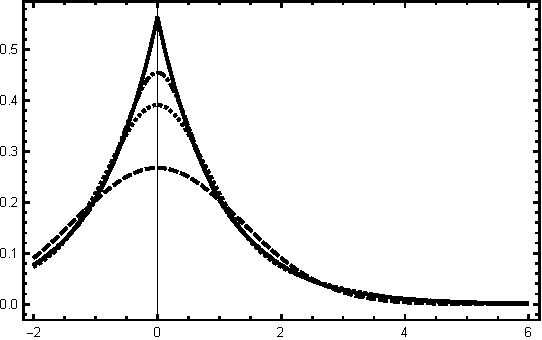
\includegraphics[height=3cm]{fig/STO_vs_GTO.pdf}
    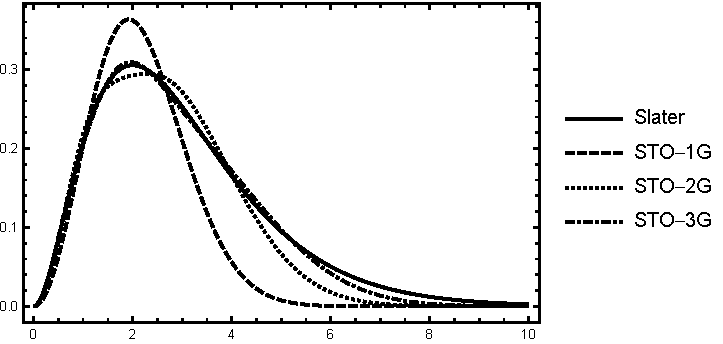
\includegraphics[height=3cm]{fig/STO_RDF.pdf}
    \caption{左图为基组,右图为基组的分布函数 $r^2\phi$}
    \label{fig:STO_GTO}
\end{figure}
% % MMA code
% Plot[{ST[1] r^2, 
%   GF[0.27095] r^2, (0.678914 GF[0.151623] + 
%      0.4330129 GF[0.851819]) r^2, (0.444635 GF[0.109818] + 
%      0.535328 GF[0.405771] + 0.154329 GF[2.22766]) r^2}, {r, 0, 10}, 
%  PlotTheme -> "Monochrome", Frame -> True, 
%  PlotLegends -> {"Slater", "STO-1G", "STO-2G", "STO-3G"}, 
%  PlotStyle -> Thick, FrameStyle -> Thickness[1/300], 
%  ImageSize -> Medium, PlotRange -> All]
% Export["STO_RDF.pdf", %]
%% 补充,Python 拟合 STO 基组:https://chc273.github.io/fitting-parameters-in-sto-lg/
%% 但是我用 MMA 就没有拟合出来,Szabo 书里的重叠积分没有 r^2 但应该有的。问题在于,两个 GTF 是完全等价的,总感觉这个搜索范围有点大(还有简并),很难把系数优化到最小 %% 放弃 %% 2022-11-29 19:48:03 Wenbin FAN @FDU

\chat{%
长程衰减速度不同,导致基组会影响渐进行为。
% 2022-11-28 08:29:15  Wenbin Fan @FDU
对电子比较弥散的系统,如阴离子束缚态,衰减快的 GTF 可能难以描述。阴离子的电子分布在原子的较外层,长程行为决定了体系跳出束缚态成为里德堡态的可能性。
% 非谐效应很重要 %% 跟非谐啥关系呢? %% 2022-11-29 21:19:20 Wenbin FAN @FDU
什么是阴离子束缚态?比如某体系有很强的偶极,当我们注入一个电子,电子最可能会出现在正极一侧。\ce{HF} 是一个典型,外侧可能会有一大团非常弥散的电子,这要求基组必须能正确描述波函数之间的长程相互作用,GTF 就会描述不好这种体系。
(助教注:这里应该是想说 dipole-bound state。加电场也可使得电子离域,当电场特别大时,电子可能会逸出,见 sobereva.com/570)
}

\chat{%
实际上,我们有办法直接用原子轨道基函数,那么为什么还要去拟合 GTF 呢?还是因为有解析结果。哪怕四中心积分存不下了,宁可 on-the-fly 即时计算,也要用 GTF。随着体系增大,四中心电子积分所需的内存量呈指数增长,一般来说是内存是放不下的,现在基本上都是即时计算的。

计算原子轨道基函数的积分有非常现实的困难。STO 不像 GTO 有解析解,STO 只能是格点积分。算一个 GTO 积分需要 \SI{1e-5}{\second},但数值的格点积分就需要 \SI{1e-2}{\second},慢了 \num{1000} 倍,这是根本不能承受的。现在确实有原子轨道基函数的程序,
% 比如 MS, Molcas (?) %% 搜了 atomic orbital integral direct 没有看到啥软件,这里就不写了 % 2022-11-29 22:21:27 Wenbin FAN @FDU
那么是用了什么技巧来节约时间呢?我们知道,四中心电子积分是四阶张量,如果用数学的方式把它降到三维或者二维,那积分结果直接就能放在内存里了。这种降维带来的优化是很恐怖的,比如原来的四中心积分需要 $\SI{100}{TB} = \SI{1e14}{bytes}$ 内存,降维成三维后只需要 $(\num{1e14})^{3/4}\,\text{bytes} = \SI{3.16e10}{bytes} = \SI{31.6}{GB}$,如果降维成二维,更是仅需 $\SI{1e7}{bytes} = \SI{10}{MB}$。原来只有超算才能算得动,现在台式机甚至是移动终端都可以算,这就是技术的进步,使得现阶段基组的选择空间就大了很多,这也是数值模拟中占比很高的研究内容。
}

\chat{%
返回来说,寻找基函数的时候另外还有个问题。量子力学基本假设说,
% 2022-11-28 08:33:55  Wenbin Fan @FDU
体系波函数最好是由具有相同边界条件的完备基展开,那么 Gaussian 型基函数是完备的吗?并不是的。完备集必须同时描述束缚态和解离态,但 GTF 显然不能描述解离态,我们刚讨论了电子完全解离的情况。
% 但 GTO 描述不了解离行为。
特别在高阶激发的时候,轨道形似解离态,波函数的行为像平面波,这是 GTO 无法描述的,GTO 不可能包含这样子的轨道。

对于一个原子的体系,可由角动量 $\hat L$ 展开得到完备集,是精确的。
% 【】完备的,角动量,指标展开得到完备基。
多个原子呢?需要用原子轨道的线性组合。两个原子上的原子轨道相互之间一定不会正交,因为有重叠,但是一个原子内的 GTF 可能是正交的。成键轨道就是两个原子上的原子轨道相互之间重叠很大,特别是共价键。
只要是分子体系,GTF 都不是完备基。
构造基组是个非常大的学问。

换句话说,如果我们遇到一个体系,现有的基函数表现不好,可否增加基函数来提高精度?实践经验告诉我们这是个非常有效的方法。再比如,post-Hartree--Fock 方法计算,波函数收敛非常非常慢,本质在于需要考虑 $1/r_{12}$ 的相互作用。
% 2022-11-28 08:40:07  Wenbin Fan @FDU
当两个电子靠近时,波函数有尖峰。现在所有的基组,都无法描述这个尖峰。轨道之间是相乘的,线性组合的原子轨道构造出的波函数,其中不会显式地出现 $1/r_{12}$,永远无法精确描述。如果增大基组,这导致数值不稳定、收敛困难。所以另有方法引入了距离,如二级微扰 MP2-F12、CCSD(T)-F12。

退回到基组本身,一直增加 GTF 到无穷多也可以是完备的,但不能实现。有没有完备基组呢?有的,凝聚态物理中常用的第一性软件 VASP 中用到的\textbf{平面波}基组就是完备的,而且平面波的动量是连续的。注意到 VASP 要求输入截断能 cutoff,这相当于我们取了从 0 到截断能这一段的平面波去展开波函数,如果不足以描述,增大截断能即可。

对于分子而言,理论上可通过平面波的组合以给出定域 local 的形式,
因为平面波是全空间等价的。
% 平面波可以描述尖点,但需要无穷多个平面波。
平面波的优点是适合描述长程行为,但是同样地靠近原子核的 cusp 难以描述。
% 【】
平面波如何处理内核电子?这就需要\textbf{赝势} pseudo-potential 将内层电子简化,本来内层电子的势能有剧烈变化,赝势则是用平滑的函数构造了内层电子并连接到价电子部分。

此外,对于同一个体系,所需的平面波数量要远大于 Gaussian 型基函数,比如一氧化碳 CO,只需要 20 个 GTF,但需要 \num{20000} 个平面波。
如此大量的基函数,会产生一个超大的稠密矩阵,对角化稠密矩阵也是个困难的问题。不同领域用不同的基函数,都有各自的难点。很自然地,有课题组开发了平面波和 GTF 结合的基组,使得 GTF 能嵌入到平面波基组中,这也是长久以来的研究方向。
% 有没有既又?小波基组,【?】混合基组。这有很多方向。
我们课题组也有过该领域的研究,如果感兴趣,欢迎加入我们。
}

\extraInfo{研究范式}{
从科学研究范式来说,1500 年前的炼金术是实验科学,牛顿等人构建起的经典物理是理论科学。从物理到化学到工程应用,实践越来越需要理论的指导。
% 是模拟科学。

从 1950 年开始,计算机开始发展。如果没有现代计算机、没有计算科学,人们不可能对微观世界有定量的认识,三个原子已经极难手工计算了,老一辈科学家手算氢弹是很令人敬佩的。计算化学已经成为了独立的学科,是一种重要的研究方式。

最新的研究方式是大数据科学、人工智能,这是一个不断进化的过程,背后反映出数学理论的进步、计算硬件的发展。
% 2022-11-28 08:49:59  Wenbin Fan @FDU
% 掌控大自然。数学工具,计算工具,基于各种工具的研究范式。
有了各种理论和工具,才能更好地理解和掌控大自然。
% 当然技术是双刃剑
}



\courseTime{Nov 28, 10th, 2 of 4}
\chat{%
继续上课。

微扰相对于变分,是另外一套用来数值逼近的方式。
微扰和变分都是计算科学中重要的原理,下周还会讲密度泛函理论,再下节课讲多电子体系。多电子体系又是另外一个世界,还要引入自旋,从多电子体系开始才算是真正买入量化计算的门槛。很可惜,我们这门课只能讲到密度泛函理论,后续内容在研究生的量化课上会继续讲。

薛定谔方程不能精确求解,变分法的目标是寻找尝试波函数。近期数学领域张益唐教授的工作非常热门,其核心思想是,将原来的大海捞针,变成了在大海的子集中找到一根针,后人可不断扩大这个子集。变分有点像大海捞针,不断构造合适的尝试波函数,实际上两个电子的变分已经很困难了,何况多电子体系。
}

% 变分法,不断扩大【】

微扰法告诉我们,复杂的体系没法求解,但是可以找到一个跳板去间接处理。假设有个体系
\begin{align}
    \hat H_0 \psi_n^{(0)} = E_n^{(0)} \psi_n^{(0)}
\end{align}
可以精确求解,同时 $\hat H - \hat H_0 = \hat H'$ 是微小差别,那么可微扰求解。构造微扰途径,线性的是最常用的,相当于 $\hat H_0$ 和真实体系的纽带,
\begin{align}
    \hat H(\lambda) = \hat H_0 + \lambda H',
\end{align}
因此薛定谔方程可以写为
\begin{align}
    \hat H(\lambda) \psi_n(\lambda) = E_n(\lambda) \psi_n(\lambda), 
\end{align}
波函数和能量可以展开为
\begin{align}
    &\psi_n(\lambda) = \psi_n^{(0)} + \lambda \psi_n^{(1)} + \lambda^2 \psi_n^{(2)} + \cdots, \\
    &E_n(\lambda) = E_n^{(0)} + \lambda E_n^{(1)} + \lambda^2 E_n^{(2)} + \cdots, 
\end{align}
其中,上标 $(k)$ 表示 $k$ 级校正。

\textbf{非简并的微扰理论},
\begin{align}
    &E_n^{(1)} = \langle \psi_n^{(0)} | \hat H' | \psi_n^{(0)} \rangle = H_{nn}', \quad H_{ij} = \langle \psi_i^{(0)} | \hat H' | \psi_j^{(0)} \rangle, \\
    &\psi_n^{(1)} = \sum_{j\neq n} \frac{\langle \psi_j^{(0)} | \hat H | \psi_n^{(0)} \rangle} {E_n^{(0)} - E_j^{(0)}} \psi_j^{(0)} = \sum_{j\neq n} \frac{H'_{jn}}{E_n^{(0)} - E_j^{(0)}} \psi_j^{(0)},\\
    &E_n^{(2)} = \langle \psi_n^{(0)} | \hat H | \psi_n^{(1)} \rangle = 
    \sum_{j\neq n} \frac{|H_{jn}'|^2}{E_n^{(0)} - E_j^{(0)}}, 
\end{align}

% 同学问,为什么各级微扰波函数之间正交?因为一级微扰波函数是用零级未微扰波函数展开的,所以相互之间没有关系。
% 拉格朗日展开
\section{氦原子的激发态}
氦原子的电子基态的微扰,
\begin{align}
    \hat H_0 = - \frac{\hbar^2}{2m_{\mathrm e}} (\hat \nabla_1^2 + \hat \nabla_2^2) - \frac{2e^2}{r_1} - \frac{2e^2}{r_2}, \quad \hat H' = \frac{e^2}{r_{12}},
\end{align}
波函数和能量
\begin{align}
    &\psi_1^{(0)}(\vec r_1, \vec r_2) = \psi_{\text{1s}} (\vec r_1) \psi_{\text{1s}} (\vec r_2) = \frac 1\pi \left(\frac2{a_0}\right)^3 \ee^{-\frac2{a_0}(\vec r_1 + \vec r_2)} = \psi_{\text{1s}}^2,
    \\
    &E_1^{(1)} =  \langle \psi_1^{(0)} | \hat H' | \psi_1^{(0)} \rangle = \frac 54 \frac{\hbar^2}{m_\mathrm{e} a_0^2}, 
\end{align}
则
\begin{align}
    &E_1 \approx  E_1^{(0)} + E_1^{(1)} = \left(-4 + \frac54\right) \frac{\hbar^2}{m_\mathrm{e}a_0^2} = -2.75 \,{\hbar^2}{m_\mathrm{e}a_0^2},\\
    &\psi_1 \approx  \psi_1^{(0)} + \psi_1^{(1)} = \psi_1^{(0)} + \sum_{j\neq1} \frac{H'_{j1}}{E_1^{(0)} - E_j^{(0)}} \psi_j^{(0)},
\end{align}

% 2022-11-28 09:19:18  Wenbin Fan @FDU
% 【图】
% n=2 不止这两个轨道是简并的。
\begin{table}[tp]
\centering
\caption{氦原子的电子排布}
\label{tab:he_electron_pop}
\begin{tabular}{>{\centering\arraybackslash }m{5mm} >{\centering }m{5mm} >{\centering }m{12mm} >{\centering }m{42mm} >{\centering\arraybackslash }m{2cm}}
\hline
No. & $n$ & 排布 & 图示 & 布居 \\
\hline
1 & 1 & 1s$^2$ & 
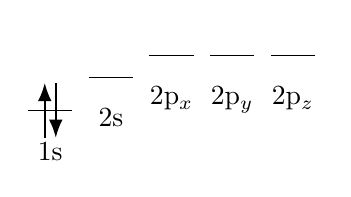
\begin{tikzpicture}[scale=0.7]
    \newcommand\w{0.8}
    \renewcommand\s{0.3}
    \newcommand\labelshift{0.4}
    \newcommand\arrowlenhalf{0.5}
    
    \fill[white, opacity=0.0] (0, 0-\arrowlenhalf-0.5) rectangle (5*\w+4*\s, 1+\arrowlenhalf);

    \draw (0,0) -- (\w,0);
    \node[below] at (\w/2,0-\labelshift) {1s}; 
    
    \newcommand\ess{0.6}
    \draw (\w+\s,\ess) -- (2*\w+\s,\ess);
    \node[below] at (\w+\s+\w/2, \ess-\labelshift) {2s};
    
    \newcommand\ep{1}
    \draw (2*\w+2*\s, \ep) -- (3*\w + 2*\s, \ep);
    \node[below] at (2*\w+2*\s+\w/2, \ep-\labelshift) {2p$_x$};
    \draw (3*\w+3*\s, \ep) -- (4*\w + 3*\s, \ep);
    \node[below] at (3*\w+3*\s+\w/2, \ep-\labelshift) {2p$_y$};
    \draw (4*\w+4*\s, \ep) -- (5*\w + 4*\s, \ep);
    \node[below] at (4*\w+4*\s+\w/2, \ep-\labelshift) {2p$_z$};
    
    % draw arrow
    \draw[->, thick, -Latex] (\w/2+0.1, \arrowlenhalf) -- (\w/2+0.1, -\arrowlenhalf);
    \draw[->, thick, -Latex] (\w/2-0.1, -\arrowlenhalf) -- (\w/2-0.1, \arrowlenhalf);
\end{tikzpicture}
&
1s(1)\,1s(2) 
\\
2 & 2 & 1s\,2s  & 
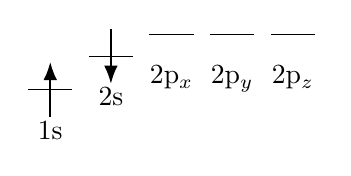
\begin{tikzpicture}[scale=0.7]
    \newcommand\w{0.8}
    \renewcommand\s{0.3}
    \newcommand\labelshift{0.4}
    \newcommand\arrowlenhalf{0.5}
    
    % \fill[white, opacity=0.0] (0, 0-\arrowlenhalf-0.5) rectangle (5*\w+4*\s, 1+\arrowlenhalf);

    \draw (0,0) -- (\w,0);
    \node[below] at (\w/2,0-\labelshift) {1s}; 
    
    \newcommand\ess{0.6}
    \draw (\w+\s,\ess) -- (2*\w+\s,\ess);
    \node[below] at (\w+\s+\w/2, \ess-\labelshift) {2s};
    
    \newcommand\ep{1}
    \draw (2*\w+2*\s, \ep) -- (3*\w + 2*\s, \ep);
    \node[below] at (2*\w+2*\s+\w/2, \ep-\labelshift) {2p$_x$};
    \draw (3*\w+3*\s, \ep) -- (4*\w + 3*\s, \ep);
    \node[below] at (3*\w+3*\s+\w/2, \ep-\labelshift) {2p$_y$};
    \draw (4*\w+4*\s, \ep) -- (5*\w + 4*\s, \ep);
    \node[below] at (4*\w+4*\s+\w/2, \ep-\labelshift) {2p$_z$};
    
    % draw arrow
    \draw[->, thick, -Latex] (\w/2, -\arrowlenhalf) -- (\w/2, \arrowlenhalf);
    \draw[->, thick, -Latex] (\w+\s+\w/2, \ess+\arrowlenhalf) -- (\w+\s+\w/2, \ess-\arrowlenhalf);
\end{tikzpicture}
& 1s(1)\,2s(2) \\
3 & 2 & 1s\,2s  & 
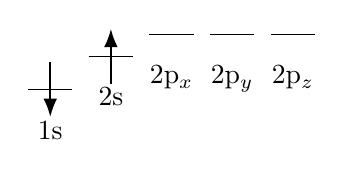
\begin{tikzpicture}[scale=0.7]
    \newcommand\w{0.8}
    \renewcommand\s{0.3}
    \newcommand\labelshift{0.4}
    \newcommand\arrowlenhalf{0.5}
    
    % \fill[white, opacity=0.0] (0, 0-\arrowlenhalf-0.5) rectangle (5*\w+4*\s, 1+\arrowlenhalf);

    \draw (0,0) -- (\w,0);
    \node[below] at (\w/2,0-\labelshift) {1s}; 
    
    \newcommand\ess{0.6}
    \draw (\w+\s,\ess) -- (2*\w+\s,\ess);
    \node[below] at (\w+\s+\w/2, \ess-\labelshift) {2s};
    
    \newcommand\ep{1}
    \draw (2*\w+2*\s, \ep) -- (3*\w + 2*\s, \ep);
    \node[below] at (2*\w+2*\s+\w/2, \ep-\labelshift) {2p$_x$};
    \draw (3*\w+3*\s, \ep) -- (4*\w + 3*\s, \ep);
    \node[below] at (3*\w+3*\s+\w/2, \ep-\labelshift) {2p$_y$};
    \draw (4*\w+4*\s, \ep) -- (5*\w + 4*\s, \ep);
    \node[below] at (4*\w+4*\s+\w/2, \ep-\labelshift) {2p$_z$};
    
    % draw arrow
    \draw[->, thick, -Latex] (\w/2, \arrowlenhalf) -- (\w/2, -\arrowlenhalf);
    \draw[->, thick, -Latex] (\w+\s+\w/2, \ess-\arrowlenhalf) -- (\w+\s+\w/2, \ess+\arrowlenhalf);
\end{tikzpicture}
& 2s(1)\,1s(2) \\
4 & 2 & 1s\,2p  & 
\multirow{3}{*}{
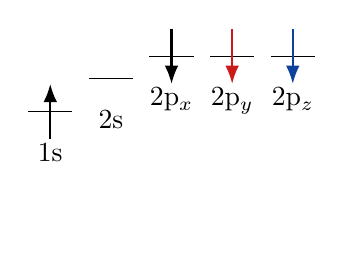
\begin{tikzpicture}[scale=0.7]
    \newcommand\w{0.8}
    \renewcommand\s{0.3}
    \newcommand\labelshift{0.4}
    \newcommand\arrowlenhalf{0.5}
    
    \fill[white, opacity=0.0] (0, 0-\arrowlenhalf-2) rectangle (5*\w+4*\s, 1+\arrowlenhalf);

    \draw (0,0) -- (\w,0);
    \node[below] at (\w/2,0-\labelshift) {1s}; 
    
    \newcommand\ess{0.6}
    \draw (\w+\s,\ess) -- (2*\w+\s,\ess);
    \node[below] at (\w+\s+\w/2, \ess-\labelshift) {2s};
    
    \newcommand\ep{1}
    \draw (2*\w+2*\s, \ep) -- (3*\w + 2*\s, \ep);
    \node[below] at (2*\w+2*\s+\w/2, \ep-\labelshift) {2p$_x$};
    \draw (3*\w+3*\s, \ep) -- (4*\w + 3*\s, \ep);
    \node[below] at (3*\w+3*\s+\w/2, \ep-\labelshift) {2p$_y$};
    \draw (4*\w+4*\s, \ep) -- (5*\w + 4*\s, \ep);
    \node[below] at (4*\w+4*\s+\w/2, \ep-\labelshift) {2p$_z$};
    
    % draw arrow
    \draw[->, thick, -Latex] (\w/2, -\arrowlenhalf) -- (\w/2, \arrowlenhalf);
    \draw[->, thick, -Latex] (2*\w+2*\s+\w/2, \ep+\arrowlenhalf) -- (2*\w+2*\s+\w/2, \ep-\arrowlenhalf);
    \draw[->, thick, -Latex, fudanRed] (3*\w+3*\s+\w/2, \ep+\arrowlenhalf) -- (3*\w+3*\s+\w/2, \ep-\arrowlenhalf);
    \draw[->, thick, -Latex, fudanBlue] (4*\w+4*\s+\w/2, \ep+\arrowlenhalf) -- (4*\w+4*\s+\w/2, \ep-\arrowlenhalf);
\end{tikzpicture}
}
& 1s(1)\,2p$_x$(2) \\
5 & 2 & 1s\,2p& & 1s(1)\,{\color{fudanRed}2p$_y$(2)}\\
6 & 2 & 1s\,2p& & 1s(1)\,{\color{fudanBlue}2p$_z$(2)}\\
\rule{0pt}{2mm}\\
7 & 2 & 1s\,2p  & 
\multirow{3}{*}{
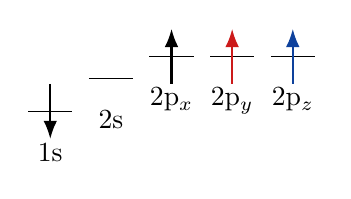
\begin{tikzpicture}[scale=0.7]
    \newcommand\w{0.8}
    \renewcommand\s{0.3}
    \newcommand\labelshift{0.4}
    \newcommand\arrowlenhalf{0.5}
    
    \fill[white, opacity=0.0] (0, 0-\arrowlenhalf-0.5) rectangle (5*\w+4*\s, 1+\arrowlenhalf);

    \draw (0,0) -- (\w,0);
    \node[below] at (\w/2,0-\labelshift) {1s}; 
    
    \newcommand\ess{0.6}
    \draw (\w+\s,\ess) -- (2*\w+\s,\ess);
    \node[below] at (\w+\s+\w/2, \ess-\labelshift) {2s};
    
    \newcommand\ep{1}
    \draw (2*\w+2*\s, \ep) -- (3*\w + 2*\s, \ep);
    \node[below] at (2*\w+2*\s+\w/2, \ep-\labelshift) {2p$_x$};
    \draw (3*\w+3*\s, \ep) -- (4*\w + 3*\s, \ep);
    \node[below] at (3*\w+3*\s+\w/2, \ep-\labelshift) {2p$_y$};
    \draw (4*\w+4*\s, \ep) -- (5*\w + 4*\s, \ep);
    \node[below] at (4*\w+4*\s+\w/2, \ep-\labelshift) {2p$_z$};
    
    % draw arrow
    \draw[->, thick, -Latex] (\w/2, \arrowlenhalf) -- (\w/2, -\arrowlenhalf);
    \draw[->, thick, -Latex] (2*\w+2*\s+\w/2, \ep-\arrowlenhalf) -- (2*\w+2*\s+\w/2, \ep+\arrowlenhalf);
    \draw[->, thick, -Latex, fudanRed] (3*\w+3*\s+\w/2, \ep-\arrowlenhalf) -- (3*\w+3*\s+\w/2, \ep+\arrowlenhalf);
    \draw[->, thick, -Latex, fudanBlue] (4*\w+4*\s+\w/2, \ep-\arrowlenhalf) -- (4*\w+4*\s+\w/2, \ep+\arrowlenhalf);
\end{tikzpicture}
}
& 2p$_x$(1)\,1s(2) \\
8 & 2 & 1s\,2p& & {\color{fudanRed}2p$_y$(1)}\,1s(2)\\
9 & 2 & 1s\,2p& & {\color{fudanBlue}2p$_z$(1)}\,1s(2)\\
\rule{0pt}{0pt}  \\ % add vertical space
\hline
\end{tabular}
\end{table}

表格 \ref{tab:he_electron_pop} 中列出了氦原子的基态和部分激发态。
\chat{%
我们已经求解了基态波函数和能量,那么怎么求解激发态呢?
% 现在我们要问个问题。1s-2s、1s-2p 的屏蔽效应不一样,那么还能简并吗?如何求解氦原子的第一激发态?
从物理上来说,1s 轨道对于 2s、对于 2p 轨道的屏蔽效应是不同的,考虑了这种屏蔽效应之后,原来简并的能级就不简并了。下面尝试求解第一激发态,这与后面的自旋有一点关联。

上次课讲过了简并能级的微扰法,需要重新讲,还是直接给答案?(同学:直接给吧,时间不太够)
}
从表格 \ref{tab:he_electron_pop} 已经得到了激发态的八重简并,对应序号 2---9。那么一级微扰波函数,需要用这 8 个简并态来展开。下面写出这 8 个零级激发的贡献,
\begin{alignat}{2}
&\psi_1^{(0)} = \mathrm{1s(1)\,2s(2)} &\quad \text{偶偶} \\
&\psi_2^{(0)} = \mathrm{2s(1)\,1s(2)} &\quad \text{偶偶}
\end{alignat}
\begin{alignat}{2}
&\psi_3^{(0)} = \mathrm{1s(1)\,2p}_x(2) &\quad \text{偶奇} \\
&\psi_4^{(0)} = \mathrm{2p}_x(1)\,2\mathrm{s}(2) &\quad \text{奇偶}
\end{alignat}
\begin{alignat}{2}
&\psi_5^{(0)} = \mathrm{1s(1)\,2p}_y(2) &\quad \text{偶奇} \\
&\psi_6^{(0)} = \mathrm{2p}_y(1)\,2\mathrm{s}(2) &\quad \text{奇偶}
\end{alignat}
\begin{alignat}{2}
&\psi_7^{(0)} = \mathrm{1s(1)\,2p}_z(2) &\quad \text{偶奇} \\
&\psi_8^{(0)} = \mathrm{2p}_z(1)\,2\mathrm{s}(2) &\quad \text{奇偶}
\end{alignat}
% \begin{align}
%     \psi_1^{(0)} = 1s(1) \ 2s(2), \quad & \psi_5^{(0)} = 1s(2) \ 2p_y(2), \\
%     [][]
% \end{align}
其中第八个波函数的表达式为
\begin{align}
    \psi_8^{(0)} = \frac1{(4\pi)^{1/2}} \left(\frac Z{a_0}\right)^{5/2} r_1 \ee^{-\frac{Z r_1}{2a_0}} \cos\theta_1 \frac1{\sqrt{\pi}} \left(\frac{Z}{a_0}\right)^{3/2} \ee^{-\frac{Zr_2}{a_0}}, 
\end{align}

\chat{%
这些内容看起来很复杂,实际上并不惜要同学们记住,如果考到了会给出公式的作为任课教师更希望同学们学到的是思维方式。日后看文献也是同理,文献不可能全部看完的,更不可能都记住,必须要在文献中找到找到所需的知识点,并尽量用起来。
% 【看文献也是】
}

简并的波函数描述成
\begin{align}
    \psi_n^{(1)} = \sum_{i=1}^8 c_in \psi_i^{(0)}, \quad i=1,\cdots,8,
\end{align}
其中的展开系数 $c_{in}$ 对应久期方程,
\begin{align}
    \left|\begin{matrix}
        H'_{11} - E_1^{(1)} & H_{12}' & \cdots & H'_{18} \\
        H'_{21} & H'_{22} - E_2^{(1)} & \cdots & H'_{28} \\
        \vdots & \vdots & \ddots & \vdots \\
        H'_{81} & H'_{82} & \cdots & H'_{88} - E_8^{(1)}
    \end{matrix}\right| = 0
\end{align}
我们需要求解其中的 $H_{ij}'$。
% 公式在前面已经给出来了。

这个 $8\times8$ 的矩阵太复杂,先做一些化简。(1) 容易证明 8 个轨道是正交归一的,有
\begin{align}
    \langle \psi_i^{(0)} | \psi_j^{(0)} \rangle = \delta_{ij}, \quad i,j = 1, 2, \cdots, 8. 
\end{align}
(2) 实空间的厄米算符,有
\begin{align}
    H_{ij} = (H_{ji}')^* = H_{ji}'. 
\end{align}
(3) 利用宇称(对称性),以
\begin{align}
    H'_{13} = \left\langle \mathrm{1s(1) \, 2s(2)} \middle | \frac{e^2}{r_{12}} \middle| \mathrm{1s(1)\,2p}_x(2) \right\rangle
\end{align}
为例,
对其中一个坐标分量 $x$ 反演,即 $x\rightarrow -x$,有
\begin{align}
\psi_{\mathrm{1s}}^* (+x_1, y_1, z_1) &\rightarrow \psi_{\mathrm{1s}}^* (-x_1, y_1, z_1) \\
\psi_{\mathrm{2s}}^* (+x_2, y_2, z_2) &\rightarrow \psi_{\mathrm{2s}}^* (-x_2, y_2, z_2) \\
\frac{e^2}{r_{12}} &\rightarrow \frac{e^2}{r_{12}} \\
% {\sqrt{(x_1-x_2)^2 + (y_1-y_2)^2 + (z_1-z_2)^2}}
\psi_{\mathrm{1s}} (+x_1, y_1, z_1) &\rightarrow \psi_{\mathrm{1s}} (-x_1, y_1, z_1) \\
\psi_{\mathrm{2p}_x} (+x_2, y_2, z_2) &\rightarrow \psi_{\mathrm{2p}_x}(-x_2, y_2, z_2) \\ 
\end{align}
注意到其中 $\psi_{2\mathrm{p}_x}$ 是关于 $yOz$ 平面对称的,反演后波函数为负。因为奇函数在对称区间上的积分为 0,所以这个积分为 0。

由此,将大矩阵分解成了 4 个小矩阵,
\begin{align}
\left|
\begin{matrix}
\begin{matrix}
b_{11} & H_{12}' \\ H_{21}' & b_{22}
\end{matrix} & {} & {} & 0 \\
{} & \begin{matrix}
    b_{33} & H_{34}' \\ H_{43}' & b_44
\end{matrix} & {} & {} \\
{} & {} &
\begin{matrix}
    b_{55} & H_{56}' \\ H_{65}' & b_{66}
\end{matrix} & {} \\
0& {} & {} &\begin{matrix}
    b_{77} & H_{78}' \\ H_{87}' & b_{88}
\end{matrix}
\end{matrix}
\right|=0,
\end{align}
其中
\begin{align}
    b_{nn} = H'_{nn} - E_n^{(1)}, \quad n=1,\cdots,8,
\end{align}
整个大的行列式为 0,只需要其中四个小的行列式为 0。比如第一个 $2\times2$ 的行列式,
\begin{align}
    \label{eq:he_excited_2times2}
    \left|\begin{matrix}
        H_{11}'-E_1^{(1)} & H_{12}' \\
        H_{21}' & H_{22}' - E_2^{(1)}
    \end{matrix}
    \right|=0. 
\end{align}

\chat{%
余下的内容下午再讲。徐老师今年特别忙,所以大部分课由张颖老师完成。在张老师的强烈建议下,徐昕老师会来讲最后一次课,内容是 DFT。未来几次课,张老师会快速讲一遍自旋、密度泛函理论的基本概念。上机操作的 QC 队列会保留到本学期结束。
}

\courseTime{3 of 4, 10th}
% 3 of 4
% 上午接着讲了微扰:简并微扰的应用。
我们现在的目的是求 He 原子的第一激发态。采用无相互作用的波函数作为未微扰波函数。

下面显式写出 $H_{11}'$ 和 $H_{22}'$ 的表达式,
\begin{align}
&H_{11}' = \left\langle \mathrm{1s(1)\,2s(2)} \middle| \frac{e^2}{r_{12}} \middle| \mathrm{1s(1)\,2s(2)} \right\rangle, \\
&H_{22}' = \left\langle \mathrm{2s(1)\,1s(2)} \middle| \frac{e^2}{r_{12}} \middle| \mathrm{2s(1)\,1s(2)} \right\rangle, 
\end{align}
% 2022-11-28 13:35:02  Wenbin Fan @FDU
很明显,
\begin{align}
    H_{11}' = H_{22}', \quad H_{33}' = H_{44}', \quad H_{55}' = H_{66}', \quad H_{77}' = H_{88}',
\end{align}
这里比较好理解,以 $H'_{11} = H'_{22}$ 来说,它是指「电子1 在 1s、电子2 在 2s」和「电子 2 在 1s、电子 1 在 1s」这两种组态是等价的。

以 $H_{11}'$ 为例,展开为
\begin{align}
    H_{11}' &= \iint |\psi_{\text{1s}}(\vec r_1)|^2 |\psi_{\text{2s}}(\vec r_2)|^2 \frac{e^2}{r_{12}} \,\dd\vec r_1 \dd\vec r_2 \\
    & = \iint \rho(\vec r_1) \rho(\vec r_2) \,\dd\vec r_1 \dd\vec r_2,
\end{align}
其中的 $\rho$ 是密度分布,
\begin{align}
    \rho(\vec r_1) = |\psi_{\text{1s}}(\vec r_1)|^2,
    \quad 
    \rho(\vec r_2) = |\psi_{\text{2s}}(\vec r_2)|^2,
\end{align}
由此密度视角,$H_{11}'$ 可理解为两电子间的库伦相互作用,用 $J$ 表示,即
\begin{align}
    H'_{11} = J_{\text{1s\,2s}}, \quad H_{22}' = J_{\text{2s\,1s}},
\end{align}
称作\boldtext{库伦积分}。对于 $H_{12}'$,其表达式为
\begin{align}
H_{12}' &= \iint \psi_{\text{1s}}^*(\vec r_1) \psi_{\text{2s}} (\vec r_1) \frac{e^2}{r_{12}} \psi_{\text{2s}}^*(\vec r_2) \psi_{\text{1s}} (\vec r_1) \,\dd\vec r_1 \dd\vec r_2 \equiv K_{\text{1s\,2s}},
\end{align}
定义其为\boldtext{交换积分}。总结为,
\begin{align}
&\text{库伦积分}\quad 
J_{mn} \equiv \left\langle f_m(1) f_n(2) \middle| \frac{e^2}{r_{12}} \middle| f_m(1)f_n(2) \right\rangle, \\
&\text{交换积分}\quad K_{mn} \equiv \left\langle f_m(1) f_n(2) \middle| \frac{e^2}{r_{12}} \middle| f_n(1)f_m(2) \right\rangle. 
\end{align}

继续求解上面 $2\times2$ 的小矩阵 \eqref{eq:he_excited_2times2},根据两种积分的定义,有
% % 2022-11-28 13:45:42  Wenbin Fan @FDU
% 对角元都相等。全空间积分,先后顺序无关。
\begin{align}
    \left|\begin{matrix}
        J_{\text{1s\,2s}} - E^{(1)} & K_{\text{1s\,2s}} \\
        K_{\text{1s\,2s}} & J_{\text{1s\,2s}} - E^{(1)}
    \end{matrix}\right| = 0
\end{align}
按照两种积分的定义,显然有
\begin{align}
    K_{mn} = K_{nm}, \quad J_{mn} = J_{nm},
\end{align}
那么容易解得这个行列式
\begin{align}
E_1^{(1)} = J_{\text{1s\,2s}} - K_{\text{1s\,2s}}, \quad E_2^{(1)} = J_{\text{1s\,2s}} + K_{\text{1s\,2s}},
\end{align}
% 2022-11-28 13:49:31  Wenbin Fan @FDU
因此,现在已经分解开了
% 【见照片】
表格 \ref{tab:he_electron_pop} 中第二个、第三个激发态
的两种简并。

% 2022-11-28 13:53:40  Wenbin Fan @FDU
求解出了能量,那么激发态的展开系数 $c$ 也可求得两种情况,进而得到一级微扰波函数为
% 【这个 c 是前面定义处的展开系数】
\begin{align}
&\psi_1^{(1)} = \frac1{\sqrt2} \big[ \mathrm{1s(1)\,2s(2) - 2s(1)\,1s(2)} \big], \\
&\psi_2^{(1)} = \frac1{\sqrt2} \big[ \mathrm{1s(1)\,2s(2) + 2s(1)\,1s(2)} \big]. 
\end{align}
\suppInfo{矩阵本征值和本征向量的求解}{
我们现在用到的量子力学都是矩阵表示,算符相当于方阵、波函数相当于列向量。在线性代数中,任何矩阵都有其本征值 eigenvalue 和本征向量 eigenvector,上述求解能量和波函数的过程就是求解本征值和本征向量的过程。

以简单的矩阵为例,
\begin{align}
    A = \begin{pmatrix}
        1 & 3 \\ 2 & 2
    \end{pmatrix}
\end{align}
本征值的定义是 $A_{n\times n}x_{n\times1} = mx_{n\times1}$,其中 $m$ 是本征值、$x$ 是本征向量,下标 $n\times1$ 表示 $n$ 行 $1$ 列。由此定义,写出
\begin{align}
    \begin{pmatrix}
        1 & 3 \\ 2 & 2
    \end{pmatrix}
    \begin{pmatrix}
        c_1 \\ c_2
    \end{pmatrix} = m 
    \begin{pmatrix}
        c_1 \\ c_2
    \end{pmatrix}, 
\end{align}
移项可得
\begin{align}
    \begin{pmatrix}
        1 - m & 3 \\ 2 & 2 - m
    \end{pmatrix}
    \begin{pmatrix}
        c_1 \\ c_2
    \end{pmatrix} = 0,
\end{align}
利用线性代数中的重要结论,线性方程组有解的条件是系数行列式为 0,所以
\begin{align}
    \left|\begin{matrix}
        1 - m & 3 \\ 2 & 2-m 
    \end{matrix}\right| = 0, \ \Rightarrow \ m^2 - 3m - 4 =0, 
\end{align}
解得两个本征值为
\begin{align}
    m_1 = 4, \quad m_2 = -1. 
\end{align}
下面求解本征向量。当 $m = m_1 = 4$ 时,代回本征值的定义,有
\begin{align}
    \begin{pmatrix}
        -3 & \phantom{-}3 \\ \phantom{-}2 & -2
    \end{pmatrix}
    \begin{pmatrix}
        c_1 \\ c_2
    \end{pmatrix} = 0,
\end{align}
容易解出来 $c_1 = c_2$,所以第一个本征向量为 $x_1 = c_1 (1, 1)^{\text{T}}$。同理可得,当 $m=m_2=-1$ 时,
\begin{align}
    \begin{pmatrix}
        2 & 3 \\ 2 & 3
    \end{pmatrix}
    \begin{pmatrix}
        c_1 \\ c_2
    \end{pmatrix} = 0,
\end{align}
解得 $2c_1 = - 3c_2$,第二个本征向量为 $x_2 = c_1 \big(1, -\frac23\big)^{\text{T}}$。

数学部分到此结束。上述过程,实际上是求解薛定谔方程 $H\Psi = E\Psi$ 的极简版本,将哈密顿量作用到本征波函数上,得到的是本征能量乘以本征波函数。

本例的氦原子激发态微扰也要用到这个过程。
在得到了激发态的去简并能量 $E^{(1)} = J_{\text{1s\,2s}} \pm K_{\text{1s\,2s}}$ 后,将其分别代回本征值的定义,有
\begin{align}
K_{\text{1s\,2s}}
\begin{pmatrix}
1 & 1 \\ 1 & 1
\end{pmatrix}
\begin{pmatrix}
c_1 \\ c_2 
\end{pmatrix} = 0, \quad 
K_{\text{1s\,2s}}
\begin{pmatrix}
-1 & \phantom{-}1 \\ \phantom{-}1 & -1
\end{pmatrix}
\begin{pmatrix}
c_1 \\ c_2 
\end{pmatrix} = 0, \quad 
\end{align}
于是我们可以得到两个本征波函数,即
\begin{align}
\psi_1^{(1)} = c_1 \begin{pmatrix}
    \phantom{-}1 \\ -1
\end{pmatrix}, \quad
\psi_2^{(1)} = c_1 \begin{pmatrix}
    1 \\ 1
\end{pmatrix},
\end{align}
利用归一化的条件,容易知道这两个 $c_1$ 都是 $\frac1{\sqrt2}$,于是便得到了最终的波函数。
}

接下来,六重简并可以分成 3 种加 3 种,
\begin{align}
&E_3^{(1)} = E_5^{(1)} = E_7^{(1)} = J_{\mathrm{1s\,2p}} - K_{\mathrm{1s\,2p}}, \\
&E_4^{(1)} = E_6^{(1)} = E_8^{(1)} = J_{\mathrm{1s\,2p}} - K_{\mathrm{1s\,2p}}, 
\end{align}
% 2022-11-28 13:57:17  Wenbin Fan @FDU
对应的波函数可以写成 % 哪种波函数?
\begin{align}
    & \psi_3^{(1)} = \frac1{\sqrt 2} \big[
    \mathrm{1s(1)\,2p}_x(2) - \mathrm{2p}_x(1)\,\mathrm{1s}(2) 
    \big], \\
    & \psi_5^{(1)} = \frac1{\sqrt 2} \big[
    \mathrm{1s(1)\,2p}_y(2) - \mathrm{2p}_y(1)\,\mathrm{1s}(2) 
    \big], \\
    & \psi_7^{(1)} = \frac1{\sqrt 2} \big[
    \mathrm{1s(1)\,2p}_z(2) - \mathrm{2p}_z(1)\,\mathrm{1s}(2) 
    \big], 
\end{align}
\begin{align}
    & \psi_4^{(1)} = \frac1{\sqrt 2} \big[
    \mathrm{1s(1)\,2p}_x(2) + \mathrm{2p}_x(1)\,\mathrm{1s}(2) 
    \big], \\
    & \psi_6^{(1)} = \frac1{\sqrt 2} \big[
    \mathrm{1s(1)\,2p}_y(2) + \mathrm{2p}_y(1)\,\mathrm{1s}(2) 
    \big], \\
    & \psi_8^{(1)} = \frac1{\sqrt 2} \big[
    \mathrm{1s(1)\,2p}_z(2) + \mathrm{2p}_z(1)\,\mathrm{1s}(2) 
    \big], 
\end{align}
% 已经求出了简并的一级微扰波函数。
我们用电子间的库伦排斥
\begin{align}
    \hat H' = \frac{e^2}{r_{12}}
\end{align}
部分消除了简并。
那么这个积分怎么算?上节课算了非简并的积分项,这里不再求了,直接给结果,
\begin{alignat}{2}
    &J_{\text{1s\,2s}} = \frac{34}{81} \frac{\hbar^2}{m_{\mathrm e}a_0^2} = \SI{11.42}{\electronvolt}, \quad
    &&J_{\text{1s\,2p}} = \frac{118}{243} \frac{\hbar^2}{m_{\mathrm e}a_0^2} = \SI{13.21}{\electronvolt},\\
    &K_{1s\,2p} = \frac{118}{243} \frac{\hbar^2}{m_{\mathrm e}a_0^2} = \SI{1.19}{\electronvolt}, \quad
    &&K_{\text{1s\,2p}} = \frac{224}{6561} \frac{\hbar^2}{m_{\mathrm e}a_0^2} = \SI{0.93}{\electronvolt},
\end{alignat}
% 2022-11-28 14:02:42  Wenbin Fan @FDU
库伦积分总是大于交换积分一个数量级以上,这是个非常 general 的结论。

\chat{%
图 \ref{fig:he_1st_perb_energy_level} 画出了一级微扰后的能级。从左往右看,分别是未微扰能级、考虑了库伦作用的能级、考虑了库伦和交换作用的能级、三级微扰能级。
}

\homework{\textbf{10.1} ~ 求 $J_{\mathrm{1s\,2s}}$ 积分。}
\chat{%
这个作业不太困难,相当于求非简并状态的一级微扰的贡献,所需的数学工具都已经讲过了。
}

\begin{figure}[tp]\centering
\begin{tikzpicture}[scale=0.2]
\newcommand\vertscale{4.5}
\newcommand\evscale{27.211386245988*\vertscale}
\newcommand\ejsss{34/81*\evscale}
\newcommand\eksss{32/729*\evscale}
\newcommand\ejspp{118/243*\evscale}
\newcommand\ekspp{224/6561*\evscale}
\newcommand\w{5}
\renewcommand\s{3}
% axis
\newcommand\axisleft{-\w-3*\s};
\draw[->, -Latex] (\axisleft, -\s) -- (\axisleft, \ejspp+\ekspp+\s);
\foreach \x in {0, 2, 4, 6, 8, 10, 12, 14}
{
\draw (\axisleft, \x*\vertscale) -- (\axisleft+0.5, \x*\vertscale);
\node[left] at (\axisleft, \x*\vertscale) {\x};
}

% E^{(0)}
\draw[thick] (-\w-\s,0) -- (-\s,0);
% 1s 2s
\draw[thick] (0,\ejsss) -- (\w,\ejsss);
\draw[thick] (\w+\s, \ejsss-\eksss) -- (\w+\s+\w, \ejsss-\eksss);
\draw[thick] (\w+\s, \ejsss+\eksss) -- (\w+\s+\w, \ejsss+\eksss);
\node[above] at (\w/2, \ejsss) {1s\,2s};
% 1p 2p
\draw[thick] (0, \ejspp) -- (\w, \ejspp);
\draw[thick] (\w+\s, \ejspp-\ekspp) -- (\w+\s+\w, \ejspp-\ekspp);
\draw[thick] (\w+\s, \ejspp+\ekspp) -- (\w+\s+\w, \ejspp+\ekspp);
\node[above] at (\w/2, \ejspp) {1s\,2p};
% dash
\draw[dashed] (-\s, 0) -- (0, \ejsss); % 0 -> 1s2s
\draw[dashed] (-\s, 0) -- (0, \ejspp); % 0 -> 1s2p
\draw[dashed] (\w, \ejsss) -- (\w+\s, \ejsss+\eksss);
\draw[dashed] (\w, \ejsss) -- (\w+\s, \ejsss-\eksss);
\draw[dashed] (\w, \ejspp) -- (\w+\s, \ejspp+\ekspp);
\draw[dashed] (\w, \ejspp) -- (\w+\s, \ejspp-\ekspp);

% energy level labels
\node[right] at (\w+\s+\w, \ejsss+\eksss) {$-55.4$};
\node[right] at (\w+\s+\w, \ejsss-\eksss) {$-57.8$};
\node[right] at (\w+\s+\w, \ejspp+\ekspp) {$-53.9$};
\node[right] at (\w+\s+\w, \ejspp-\ekspp) {$-55.7$};
\node[right] at (\w+\s+\w, 0) {$-68.0$};

% arrows
\draw[<->] (\w/2, 0) -- (\w/2, \ejsss);
\node[right] at (\w/2, \ejsss/2) {$J_{\mathrm{1s\,2s}}$};
\draw[<->] (-\s-\w/2, 0) -- (-\s-\w/2, \ejspp);
\node[left] at (-\s-\w/2, \ejspp/2) {$J_{\mathrm{1s\,2p}}$};
\draw[<->] (\w+\s+\w*2/3, \ejsss+\eksss) -- (\w+\s+\w*2/3, \ejsss-\eksss);
\node[right] at (\w+\s+\w*2/3, \ejsss) {$K_{\mathrm{1s\,2s}}$};
\draw[<->] (\w+\s+\w*1/3, \ejspp+\ekspp) -- (\w+\s+\w*1/3, \ejspp-\ekspp);
\node[right] at (\w+\s+\w*1/3, \ejspp) {$K_{\mathrm{1s\,2p}}$};

% more precious solution
% here 4*\s means we add 2*\s extra space
\draw[thick] (2*\w+4*\s, 0.37589*\evscale) -- (3*\w+4*\s, 0.37589*\evscale);
\draw[thick] (2*\w+4*\s, 0.36486*\evscale) -- (3*\w+4*\s, 0.36486*\evscale);
\draw[thick] (2*\w+4*\s, 0.35384*\evscale) -- (3*\w+4*\s, 0.35384*\evscale);
\draw[thick] (2*\w+4*\s, 0.32444*\evscale) -- (3*\w+4*\s, 0.32444*\evscale);
% link 1st perb to precious solution
\draw[dotted] (\w+\s+\w, \ejspp+\ekspp) -- (2*\w+4*\s, 0.37589*\evscale);
\draw[dotted] (\w+\s+\w, \ejspp-\ekspp) -- (2*\w+4*\s, 0.36486*\evscale);
\draw[dotted] (\w+\s+\w, \ejsss+\eksss) -- (2*\w+4*\s, 0.35384*\evscale);
\draw[dotted] (\w+\s+\w, \ejsss-\eksss) -- (2*\w+4*\s, 0.32444*\evscale);
% arrows
\draw[<->] (2*\w+4*\s+\w/2, 0.37589*\evscale) -- (2*\w+4*\s+\w/2, 0.36486*\evscale);
\node[right] at (2*\w+4*\s+\w/2, {((0.37589-0.36486)/2+0.36486)*\evscale}) {1s\,2p};
\draw[<->] (2*\w+4*\s+\w/2, 0.35384*\evscale) -- (2*\w+4*\s+\w/2, 0.32444*\evscale);
\node[right] at (2*\w+4*\s+\w/2, {((0.35384-0.32444)/2+0.32444)*\evscale}) {1s\,2s};
% energy level labels
\node[right] at (3*\w+4*\s+\s/2, 0.37589*\evscale) {$-57.8$};
\node[right] at (3*\w+4*\s+\s/2, 0.36486*\evscale) {$-58.1$};
\node[right] at (3*\w+4*\s+\s/2, 0.35384*\evscale) {$-58.4$};
\node[right] at (3*\w+4*\s+\s/2, 0.32444*\evscale) {$-59.2$};
\end{tikzpicture}
\caption{氦原子一级微扰后的能级。左侧坐标轴的零点是 $\SI{-2.5}{Hartree} = \SI{-68.0}{\electronvolt}$,右侧是绝对能量,单位均为 eV。左下角是未微扰能级,最右边是计算到三级微扰的能级(无交叉),中间部分是一级微扰的能级(有交叉)。}
\label{fig:he_1st_perb_energy_level}
\end{figure}

\chat{%
% 2022-11-28 14:03:54  Wenbin Fan @FDU
从谱项的角度来说,能级发生了劈裂。
% 微扰之后能量不一定下降,【图,好大一张图】
% 2022-11-28 14:07:27  Wenbin Fan @FDU
为什么库伦作用让能量上升?因为零级波函数没有相互作用(电子间的排斥)。考虑了库伦作用后,能量一定是往上拉的。
}

下面讨论一级微扰得到的谱图。
% % 2022-11-28 14:10:21  Wenbin Fan @FDU
% 【】劈裂出来的两个【?】,一定比 1s 2p 低

\textbf{1. 错误的能级交叉:}
谱图中有个很严重的问题,即 $\mathrm{1s\,2s}$ 的能级,不管是否考虑交换作用,总要比 $\mathrm{1s\,2p}$ 能级低,也就是说这两个能级存在错误的交叉,这是由于忽略的高阶项的激发导致的。
\chat{%
采用变分微扰的方式,Knight、Scherr 等人计算了二级、三级能量校正,能级不再交叉。参考文献 Scherr, C. W., \& Knight, R. E. (1963). Two-Electron Atoms III. A Sixth-Order Perturbation Study of the 1$^1S$ Ground State. \emph{Reviews of Modern Physics, 35}(3), 436. DOI: 10.1103/RevModPhys.35.436 ,这是个爷爷辈的工作。
}

% 2022-11-28 14:14:58  Wenbin Fan @FDU
考虑到库仑相互作用,则 $\mathrm{1s\,2s}$ 和 $\mathrm{1s\,2p}$ 感受到的屏蔽效应是不同的,那么这两个能级一定是会分开的。

% 2022-11-28 14:26:01  Wenbin Fan @FDU
\courseTime{4 of 4}
\chat{%
通过库仑相互作用,在一级相互作用下,就可以正确地将 8 重简并分解成 4 个态。其中,$\mathrm{1s\,2s}$ 是没有简并的两个态,$\mathrm{1s\,2p}$ 有两个三重简并的态。对这个结论的第一个思考是,通过一级微扰可以分裂能级,但一级微扰不够。幸运的是,这个微扰比较小,还可以用微扰法。
}

\textbf{2. 库伦简并的消除:}
未微扰态存在两种简并,
\begin{alignat}{2}
    &\text{$n$ 相同但 $l$ 不同}\quad &&\mathrm{2s, 2p},\\
    &\text{$l$ 相同但 $m_l$ 不同}\quad &&\mathrm{2p}_x, \mathrm{2p}_y, \mathrm{2p}_z,
\end{alignat}
% 【拍照,红圈是库伦微扰】
1s 2s 的库伦微扰更小,1s 2p 离原子核更远,受到的屏蔽更小一些,那么库伦简并就消除了。
\chat{%
同理,如果考虑了电子的相互作用,此时必须考虑激发电子 2s 和未激发电子 1s 的关系,那么我们发现 $\mathrm{1s\,2s}$ 的相互作用排斥能比 $\mathrm{1s\,2p}$ 的更小,自然就有了库伦简并的消除。

严格来说,在 1s 电子存在的时候,2s 电子的分布比 2p 电子的分布更接近原子核,因此 2s 电子受到更少的 1s 电子的屏蔽。
% 【两个说法角度不同】

屏蔽和排斥是等效的说法,更少的屏蔽表示更少的相互作用。
库伦排斥可以从一个简并态分离成两个简并态。
}

\textbf{3. 交换简并的消除:}
没有微扰的波函数是
\begin{align}
    \psi_1^{(0)} = \mathrm{1s(1)\,2s(2)}, \quad 
    \psi_2^{(0)} = \mathrm{2s(1)\,1s(2)},
\end{align}
% 本章用的 psi 应该是 phi 和 Phi % 不改了,波函数全都用 psi 吧 %% 2022-12-01 20:06:47 Wenbin FAN @FDU
一级微扰之后的波函数是
\begin{align}
    &\psi_1^{(1)} = \frac1{\sqrt2} \big[\mathrm{1s(1)\,2s(2) - 2s(1)\,1s(2)}\big], \\
    &\psi_2^{(1)} = \frac1{\sqrt2} \big[\mathrm{1s(1)\,2s(2) + 2s(1)\,1s(2)}\big],
\end{align}
微扰之后发现,这两个波函数是一加一减,已经不能区分电子在 1s 还是 2s 了。这背后对应着,
% 线性变分【】。
波函数必须能够反映量子力学体系\textbf{等同粒子的不可区分性}。

我们知道一级微扰的能量
\begin{align}
    E_1^{(1)} = J_{\mathrm{1s\,2s}} - K_{\mathrm{1s\,2s}},\quad E_2 = J_{\mathrm{1s\,2s}} + K_{\mathrm{1s\,2s}},
\end{align}
得到
\begin{align}
    E_1^{(1)} - E_2^{(2)} = - 2K_{1s\,2s}
\end{align}
称作交换简并消除。

\chat{%
% 2022-11-28 14:37:43  Wenbin Fan @FDU
交换简并消除意味着什么?为什么 $E^{(1)}_1$ 比 $E^{(1)}_2$ 小?做以下假设,当 $r_1 = r_2$ 时,
\begin{align}
    \begin{array}{l}
    \psi_1^{(1)} (r_1, r_2 = r_1) = 0, \\
    \psi_2^{(1)} (r_1, r_2 \neq r_1) \neq 0,
    \end{array}
    \Rightarrow
    \begin{array}{l}
    \rho(r_1, r_2) = |\psi_1^{(1)}|^2 = 0, \\
    \rho(r_1, r_2) = |\psi_2^{(1)}|^2 \neq 0,
    \end{array}
\end{align}
通过构造,使得两个粒子不可能出现在同一个位置。交换效应使得体系能量更稳定,消除了两个电子同时出现在同一位置的概率。如果两个电子出现在同一位置,会产生较大的库伦排斥能。相减的波函数,比相加的更稳定,因为从交换对称的角度来说,相减的波函数限制了两个电子不能出现在同一位置,后面也会学到。
% 2022-11-28 14:40:59  Wenbin Fan @FDU
% 导致更稳定,后面也会学到。

为什么交换这么重要?下节课讲自旋和多电子体系。接下来的几周没有新的量子力学内容。等同粒子有没有不可区分性?用波函数描述系统时,自然就有不可区分性,这种性质背后对应的是玻色子、费米子等不同粒子,从而引出了自旋的概念。
}

\chat{%
变分自然地能保证等同粒子的不可区分性。
% 2022-11-28 14:42:53  Wenbin Fan @FDU
% 我们讲变分的时候,
变分是说,给定尝试波函数,得到的能量永远比基态能量高。从微扰角度来说,从 \SI{-68.0}{\electronvolt} 微扰上去,一直得到各个态。但是,高级别微扰得到的 \SI{-59.2}{\electronvolt} 比 \SI{-68}{\electronvolt} 高,这有没有破坏变分原理呢?这个 \SI{-68.0}{\electronvolt} 是 $H_0$ 的本征函数,对应于 $\langle \psi | H_0 | \psi \rangle = E_1$,是我们对精确哈密顿进行处理的,哈密顿量没有近似。微扰中是近似哈密顿,近似哈密顿的基态能量,不能保证比真实哈密顿的基态能量要高,这里的氦原子就是个典型粒子。氦原子的零级哈密顿量是两个完全独立电子的哈密顿量相乘,完全不考虑排斥作用。这个哈密顿量的好处是什么呢,不含库伦排斥的哈密顿量求出的能量更低。变分原理在微扰情况下,不能保证微扰波函数对应的期望能量比体系的基态能量低。%【返回 非简并微扰理论】

假设,我们把尝试波函数代回到真实的哈密顿量 $\langle \psi^{\text{trial}} | \hat H | \psi^{\text{trial}} \rangle \geqslant E_0$,再代回未微扰哈密顿量 $\langle \psi^{\text{trial}} | \hat H_0 | \psi^{\text{trial}} \rangle = E_1$,
能否保证 $E_1$ 一定小于 $E_0$?这个没法保证,因为没做变分。以经验来说,偶数阶的微扰能量更低,奇数阶的微扰能量高于真实能量,所以量化计算中常用的微扰理论方法是二阶微扰 MP2,也有利用二阶三阶微扰混合形成的 MP2.5。
}

\homework{\textbf{10.2} ~  氢原子受 $z$ 轴方向均匀外加电场微扰时,其微扰 $\hat H' \equiv e \vec A = e A \, r \cos\theta$,其中 $A$ 是电场强度。考察 $\hat H'$ 对 $n=2$ 能级的影响。这个能级是四重简并。因为 $\hat H'$ 与角动量算符 $\hat L_z$ 是对易的,可利用 2p$_{0}$、2p$_{-1}$ 建立久期行列式,并利用宇称证明部分 $\hat H'$ 矩阵元素为零。求非零积分、能量一级校正、正确的零级波函数。}
\chat{%
这个题目比氦原子稍微简单,这里只有一个电子,从 1s 激发到 2s、2p 上。
}

\chat{%
到这里,微扰算是讲完了。我们涉及到的粒子只有一个或两个。一旦涉及多个粒子,就会出现全同粒子可否区分的问题,而全同粒子一定会演化出自旋的讨论。因为时间有限,本来应该要继续这部分内容讲,但是考虑到重要性,先讲密度泛函理论。
}

\chapter{密度泛函理论}
% %2022-11-28 14:56:55  Wenbin Fan @FDU
% 原来我想讲的是密度泛函理论。一旦讲到 DFT 就涉及到多电子体系,【】
\section{密度泛函理论的发展}
密度泛函理论 density functional theory (DFT) 涉及到的是多电子体系。

\chat{%
大家听过密度泛函理论吗?字面理解是啥意思?(同学:HK 存在定理)大家八九不离十都能讲点东西。
}

\begin{figure}[tp]
    \centering
    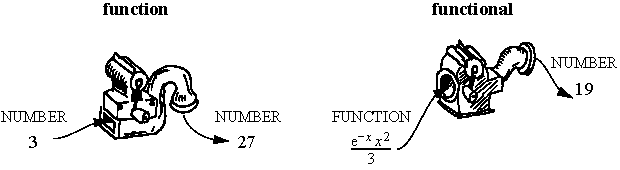
\includegraphics[height=3cm]{fig/fct_fctn.pdf} 
    \caption{函数和泛函的区别,选自 Lancaster, Tom, and Stephen J. Blundell. \emph{Quantum field theory for the gifted amateur}. OUP Oxford, 2014.}
    \label{fig:function_vs_fuctional}
\end{figure}
泛函是什么意思?函数的函数,输入一个函数得到数值,那么函数是数值到数值的映射。DFT 里的泛函是波函数作为输入,我们要找到一个波函数让能量最低。如图 \ref{fig:function_vs_fuctional}。

\chat{%
密度泛函,毫无疑问是指用密度映射能量,即基态能量可以由基态密度唯一确定,这是密度泛函的基本原理。

这个原理有什么好处?我们求薛定谔方程,不考虑自旋、时间,波函数 $\psi$ 是 $N$ 个电子 $3N$ 维度的变量,波函数的构造是很复杂的,而且波函数没有物理意义。密度是什么概念?粒子是不可区分的,在任意一点找到电子的概率即密度。如果全空间有 $N$ 个电子,那么密度的全空间积分为 $N$。

密度 $\rho$ 是 3 维,但波函数是 $3N$ 维的。密度的求解远比薛定谔方程求解简单。如果能找到密度和能量的映射关系,那么就有更简单的方式求解薛定谔方程。

这就是我希望把 DFT 放在变分微扰后面紧接着讲的原因,因为密度泛函理论并没有超出求解薛定谔方程,无非是重构薛定谔方程的方式。变分是寻找尝试波函数,微扰是利用未微扰波函数作为跳板。

DFT 是一种不走寻常路的形式,跳出波函数去寻找密度。
}

DFT 中最基本的 Hohenberg--Kohn 定理下节课再讲。先尝试从变分推导,
% 2022-11-28 15:03:43  Wenbin Fan @FDU
通过变分看看有没有这种可能性。做\textbf{限制性变分},
\begin{align}
    \langle \psi | \hat H | \psi \rangle |_{\text{min}} = E_0,
\end{align}
% 【】假设知道全空间【?】
这里做了一些理论上的假设,即全体尝试波函数是已知的,那么才能得到上面的等号。

% 2022-11-28 15:04:51  Wenbin Fan @FDU
假如我们有一种很聪明的方式,把波函数的变分空间按所需的方式做任意的组合,我们可以组合出一组 $\{\psi_{\rho_1}\}, \{\psi_{\rho_2}\}, \cdots$ 子空间,它们能给出
密度相同的波函数,
这个子空间构成了 $\big\{\{\psi_{\rho_i}\}\big\} = \{\psi\}$。这种做法仅是从理论上可行,因为波函数空间可以说是无穷大,实际上难以取出所有密度相同的波函数。
% 2022-11-28 15:06:26  Wenbin Fan @FDU
有了这个做法之后,变分就成了最小化具有相同密度下的波函数所对应的能量,
% 找所有的最小。
\begin{align}
\left\{
\begin{array}{l}
\langle \psi_\rho | \hat H |\psi_\rho \rangle|_\text{min} = E[\rho], \\
E[\rho] | _{\text{min}} = E_0
\end{array}
\right.
\end{align}
这里第一行是说,在我们假设变分空间里所有波函数的密度都相同的情况下,最小化「密度函数到能量」这个泛函,最小化得到的是密度函数,第二行是最小化这个密度函数,得到了能量。
换句话说,的确可以将体系能量表示能密度的函数。

% % 2022-11-28 15:07:14  Wenbin Fan @FDU
% 确实可以找出来 $E_0$,

把波函数再展开,
\begin{align}
    E[\rho] = 
\langle    \psi_\rho | \hat T + V_{\mathrm{ee}} + V_{\mathrm{ext}} | \psi_\rho \rangle | _{\text{min}}  
= F[\rho] + V_{\mathrm{ext}}[\rho], 
\end{align}
因为 min 走遍了所有密度相同的波函数,那么动能和库伦项都是相等的,所以动能算符和库伦算符构成了普适泛函。
\chat{%
换句话说,密度泛函的的存在性不需要 HK 定理证明,可以通过限制性变分搜索来证明密度到基态能量的映射关系是存在的。
% 通过限制性搜索,证明密度到能量的映射关系是存在的,
一旦映射关系找到了,我们要去搜索所有的密度,其中最低的能量就是基态能量。如果能构造一个泛函,使得该泛函输出给定密度的最小值能量,那么对密度进行变分可得到体系的基态能量。这个有点超纲了,这里的推导是想说,
如何用变分法从密度给出密度的映射关系,没有任何的数值可行性。

% 2022-11-28 15:10:51  Wenbin Fan @FDU
变分法是构造尝试波函数空间,微扰法是去寻找合适的零级无微扰波函数,密度泛函是为了找到更好的映射关系,进而操作密度而不是波函数得到体系精确的能量。DFT 不对波函数进行操作,但密度不是波函数,密度不包含体系的所有信息,密度不包含微妙的量子耦合等,相当于对体系的全部信息做了取舍,用精度换取计算量,天下没有免费的午餐 no-free-lunch theorem。

上课上到 Dec 19 Mon。还有三次课。我跟大家保证,如果平时作业认真做,最后一定会过的。考试难度只有平时的 70 80\%。本课的出发点不是像高考一样选拔。希望同学们理解化学中背后的物理,当然这离不开数学基础。
}
\courseTime{Dec 05, 11th}
\chat{
今天到场的同学有点少啊(只有 8 位同学),看来我们要点名了。

我们还有 3 次课(算上本次),最后一次课徐昕老师来讲密度泛函,他会从头开始讲密度泛函的原理和发展。

先来回顾前面三次课讲的内容,主要是微扰和变分。本课是量子化学的基本原理和应用,跳出课程来看,化学科研的三种基本手段是实验、理论和模拟,从课程属性来看应当归到理论中,事实上任何理论想要真正地解释和指导实验,都必须要用计算机模拟。

本课讲过了量子力学基本原理和公设,也推导为数不多的可解系统,我们会发现,稍微复杂一点的体系就没有精确解,那么由此诞生了数值模拟,即通过数值近似去求解复杂系统。既然有近似就有误差,现代数值模拟可以说是精度和效率之间平衡的艺术。

借助计算机的快速发展,目前基本实现了通过数值模拟连接了实验和理论,也可以说数值模拟填平了理论和实验之间的鸿沟,让理论走在实验的前方,未来也必将实现用理论去设计实验的终极目标。所以,量子化学的大方向是基于量子力学基本原理的数值方法的开发,从这个角度来说,本课前面的所有内容都可以归纳到数值模拟的范畴,相信同学们在物化课上都已略知一二。
}

我们讲变分和微扰,根本原因是薛定谔方程不能精确求解,
\begin{align}
    \hat H \psi = E \psi,
\end{align}
这里写出的是定态、不含时、非相对论的薛定谔方程,这儿有很多约束条件。% 2022-12-05 12:47:01  Wenbin Fan @FDU
\chat{
因为一旦其中的势函数显含时间或时间空间不能分离,那就不能得到定态薛定谔方程。幸运的是,人们感兴趣的很多化学性质,都是能由定态薛定谔方程求解出来的。诚然,一旦涉及到动力学性质等,薛定谔方程就不够用了,需要用含时薛定谔方程。话说回来,变分和微扰是求解薛定谔方程的方法,必然会考。}

变分法说的是,能量的期望值总是可以写成
\begin{align}
    \bar E = \frac{\langle \psi | \hat H |\psi\rangle}{\langle \psi | \psi \rangle} \geqslant E_0,
\end{align}
变分原理告诉我们能量大于等于 $E_0$,其中的 $\psi$ 是试探波函数,试探波函数必须满足哈密顿量的边条件。
\chat{这里包含了量子力学中两个最基本的假设。第一,微观粒子的所有行为都由波函数表述。我们如何从波函数中抽提出物理可观测量?讲该可观测量所对应的算符作用在波函数上,如果这个算符是可观测量的本征函数,那么就得到了本征值,如果不是本征函数,那么可以积分得到期望值。

变分法很有趣。如果我们将变分法当作原理,可以看出变分法给出了一条探索体系基态能量的途径。这是从物理角度来说的,如果从数学角度切入,或者从量子力学基本原理阐述,变分法将薛定谔方程这个偏微分方程,转化成了积分的方程,并找到了波函数与基态能量的映射关系,这种映射关系也可以称作泛函。

什么是泛函?我们知道函数是 $x \xrightarrow{f} y$ 数值到数值的映射,泛函是函数到数值的映射。从更朴素的角度来说,函数或泛函的映射关系,相当于以某种方式消除了自变量,在变分法中,这种消除方式是全空间积分。

用变分法求解能量的极小值,相当于寻找``试探波函数-能量''泛函上的极小值。这里为什么不说是最小值,因为人们通常不可能掌握一个高维函数的全部信息,找到极小点仅相当于井底之蛙,在井底是不可能知道旁边是否有更深的井。更严格地说,寻找全局最小值是个 NP 问题。

实践当中,通常都以优化极小点为目标,部分课题组致力于探索完整的势能面空间。只要初始猜测足够接近极小点,都是可以优化到极小点的。这里的足够接近,定义是在极小点的二次区域内,只要在这个区域内,这些利用二阶导数的优化算法均可以顺利优化到极小点。

在变分法中,这个实际的优化问题就变成了怎么设计初始猜测波函数。我们已经在在上机课中体会到了,只要我们设定好简单的参数,如坐标、电荷、自旋多重度,Gaussian 程序包自动就能算好波函数和能量。如此自动化的程序,背后蕴藏着几代科学家数十年的心血。即使你不懂什么是初猜,不懂任何数值算法,简单几步就能在计算机中模拟一个分子。现代量化软件越来越稳定,成为了黑箱。
% 很多实验组买了量化软件,简单学习软件操作后就可以迅速上手计算。

当我们用量化软件模拟得到光谱等可观测量,唯一需要考虑的是当前结果的不确定性有多大,可以在多大的置信范围内解释实验。所以,量化软件就相当于实验仪器,而且是非常稳定的仪器。
}
\suppInfo{驻点的分类}{
在应用了 BO 近似后,体系的势能由原子核坐标决定,由此产生了势能面 potential energy surface 的概念。如果体系有 $N$ 个电子,那么势能是 $3N$ 维度的函数,如果不考虑平动和转动,则势能是 $3N-6$ 维度的函数。这种高维函数通常无法直接可视化,也被称作超曲面 hyper-surface。

势能面上仅有个别区域是人们关注的,比如对应于稳定结构的极小点、对应于过渡态的鞍点,以及连接极小点和鞍点的反应路径。极小点和鞍点都是数学中一阶导数为 0 的点,且极小点的二阶导数为正,鞍点的二阶导数仅有一个负的本征值。对于函数的极小点,必须满足
\begin{align}
\pdv{E}{\lambda} = 0, \ \text{且} \ \pdv[2]{E}{\lambda} \geqslant 0. 
\end{align}
数学上极小点的判定条件,同样也可以应用在变分法中。

能量的二阶导数是力 $F = - \nabla V$,极小点要求二阶导数为正,通俗地说就是任意方向都是开口向上的函数。
}

% % 2022-12-05 08:20:03  Wenbin Fan @FDU
% 量化程序,黑箱
% uncertainty,仪器
% 如何提高精度?

变分法的困难,如何更有效地构建符合边界条件的初猜波函数 $\{\psi\}$。
\chat{波函数包含体系的所有信息,必须是 $3N$ 维度的,往后学习了自旋还要加入自旋维度,所以实际上是 $4N$ 维的。构造如此高维的空间是很困难的,当然了,搜索这个高维空间也很困难,所以我们需要线性变分法。

接下来还有更复杂的组态相互作用,逐渐逼近真实的解,但是这个逼近过程所消耗的计算资源是急剧增加的。以朴素的单电子近似方法 Hartree--Fock 为例,它的计算标度 scaling 是 $N^4$,这里的 $N$ 是基函数的个数。我们在前面推导过,\num{10000} 个水的系统就要耗时数百年,遑论标度更高的方法了。
% full-CI 是指数增长的。

这种指数增加的耗时是非常恐怖的。如果把加法比作一级增长,那么乘法是二级增长、乘方则是三级增长,近期知乎上的热门话题葛立恒数 $G(64)$ 则是第四级的超乘方,很多网友试图构造超越葛立恒数的大数,实际上连 $G(1)$ 都没有超越。

量子化学中,特别是电子结构计算中,这种指数增长被形象地称作``指数墙''。指数函数的图像的尾巴会急剧增长,这像一堵墙一样挡住了往更大体系的去路。张颖老师开发了适用于超大规模并行的 CCSD(T) 程序,在 \num{10000} 个核心上取得了超过 80\% 的效率,相当于将耗时减少了 4 个数量级,也就是耗时从 1 个月变成了 $\sim$320 秒。尽管这是个振奋人心的成就,但是在指数墙面前依然杯水车薪,哪怕是再增加一个电子,很可能这辈子都算不完了。

现代计算机工业经过了几十年的蓬勃发展,到目前为止摩尔定律依然有效,超级计算机占据了大国博弈的主战场,中美双方``你方唱罢我登场''。现阶段唾手可得的氢分子模拟,在 30 年前是难以想象的计算量。

简单举一个例子,如果要储存 10 个电子的波函数,需要消耗多少内存,再增加一个电子需要多少内存?假设每一个维度有 20 个点(或者说划分成 20 个格),每个格点消耗 \SI{1}{bytes},那么 10 个电子的波函数需要消耗 $20^{4\times 10}\,\text{bytes} = \SI{1.10e52}{bytes}$,11 个电子的波函数需要消耗 $20^{4\times 11}\,\text{bytes} = \SI{1.76e57}{bytes}$,增长了 $20^4 = \num{160000}$ 倍。
}

% % 2022-12-05 08:26:50  Wenbin Fan @FDU
% 背后原因是波函数过于复杂。

\textbf{微扰法}是一种``分而治之''的方法,因为直接求解不现实,所以分步达到目标。核心思路有两条,第一是构造与真实波函数有相同边界条件的零级哈密顿量,
\begin{align}
\hat H_0 \psi_n^{(0)} = E_n^{(0)} \psi_n^{(0)}
\end{align}
可以精确解,第二是近似哈密顿与真实哈密顿的差足够小,
\begin{align}
    \hat H' = \hat H - \hat H_0,
\end{align}
\chat{
一口吃不成个胖子,一步也没法登上月亮,但是为了登上月亮,人们可以先爬上摩天大楼的楼顶,当然这个摩天大楼和地月距离的对比有些夸张。

第一点边界条件的要求是为了用这一组零级波函数展开真实波函数,第二点微扰足够小的要求是确保高级别微扰收敛。如果一级微扰都会发散,微扰就没有意义了。
}

有了微扰的定义,再引入\boldtext{线性变分},
\begin{align}
    \hat H(\lambda) = \hat H_0 + \lambda \hat H', \quad \lambda \in[0,1],
\end{align}
其薛定谔方程为
\begin{align}
    \hat H(\lambda) \psi_n(\lambda) = E_n(\lambda) \psi_n(\lambda),
\end{align}
可以严格地写出其波函数和能量,
\begin{align}
&\psi_n(\lambda) = \psi_n^{(0)}(\lambda) + \lambda\psi_n^{(1)}(\lambda) + \lambda^2 \psi_n^{(2)}(\lambda) + \cdots, \\
&E_n(\lambda) = E_n^{(0)}(\lambda) + \lambda E_n^{(1)}(\lambda) + \lambda^2 E_n^{(2)}(\lambda) + \cdots,
\end{align}
当 $\lambda \rightarrow 1$ 时,可得真实体系的能量。
% 2022-12-05 08:31:18  Wenbin Fan @FDU
% 2022-12-05 08:31:43  Wenbin Fan @FDU
\chat{
用线性变分法,不再有构造边界条件的困难,因为我们已经通过零级哈密顿量构建了展开真是波函数所需的辅助基函数。
}
微扰的困难在于如何合理地构建 $\hat H_0$ 使之更接近于 $\hat H$。
\chat{
这包含了两层目标,第一是为了微扰更快地收敛到真实解,如果 $E_n^{(0)}$ 更接近真实能量,那么就可以算更少的微扰项。第二个是更基本的问题,为了使得 $H_0$ 接近 $H$,以便在数学上展开合理,也就是 $\lambda \in [0,1]$ 不能超出波函数和能量的收敛半径。特别在强关联体系中,需要考虑,人为选定组态波函数,才能继续做微扰。

刚才用半小时梳理了变分和微扰,因为期末考试会有近似方法的大题。不用担心,所有的技术细节不会超出作业的难度。

变分和微扰都是\textbf{数值求解}薛定谔方程的方法,各有优劣。有无其它方式逼近薛定谔方程的解呢?现在我们讲一种新的方法——\textbf{密度泛函理论}。最后一次课由徐昕老师讲授密度泛函理论,预计内容会非常丰富。为了帮助理解,接下来先铺垫一些密度泛函理论的基本概念,以便同学们在最后一次课能畅快地理解。
}

\section{DFT 基础}
\chat{
前面复习了两种基于波函数的近似方法——变分和微扰。变分法的思路是将薛定谔方程这一偏微分方程转化成波函数积分的泛函,使得能量成为波函数的泛函。
}
体系能量 $E$ 可以是体系密度 $\rho$ 的函数吗?
\chat{
如果从波函数入手,并不能直接推知。但这个想法持续吸引着人们,因为波函数实在太复杂了,不考虑自旋已经是 $3N$ 维的。人们需要一种更简单的方式求解薛定谔方程。
}
% 波函数方法,是【?】
% 能量一定是波函数的函数,这是按照定义得到的。那么,能量可以是体系密度的函数吗?如果我们从波函数的函数来看,其实这并不能直接推导出来。为什么这个想法从一开始就这么吸引人?我们讲过波函数最大的问题是太复杂了!不考虑自选都有 $3N$ 维度的,但是
密度是空间中任意一点找到电子的概率,只有 $3N$ 维,全空间积分
\begin{align}
    \int \rho(r)\,\dd r = N. 
\end{align}
\chat{密度不同于波函数。波函数不是物理可观测量,但电子密度是可观测量,比如通过 X 射线``打出''电子分布。

从密度得到能量,这个想法非常具有吸引力。具体如何实现?
}

我们遇到的第一个问题是,什么是密度?
\chat{
哥本哈根统计学派告诉我们,波函数模的平方是概率,
\begin{align}
|\psi(\vec r_1, \vec r_2, \cdots, \vec r_N)|^2 \,\dd \vec r_1\, \dd\vec r_2 \cdots \dd\vec r_N,
\end{align}
这个概率是否是密度?并不是。
波函数的模方指``在 $\dd r_1$ 位置找到第一个电子、在 $\dd\vec r_2$ 找到第二个电子、……在 $\dd \vec r_N$ 找到第 $N$ 个电子''的概率。所以,波函数一旦写成函数形式,每个电子在波函数中的位置是固定的、电子在波函数中的排序是隐含的变量。
% 就是变量可以写成 r1 r2 rn,也可以互换,本身变量的位置隐含着【】,顺序是不会变的,
% 电子是可区分的,第一个变量对应第一个电子,这是函数中约定的概念。
这个还是蛮复杂的,Igor 当年就搞混了。
% 波函数的模方指的是 $N$ 个电子分别出现在 r1 r2 ... 的概率。
}
由于粒子的不可区分性,精确的多体波函数必须满足
\begin{align}
|\psi(\vec r_1, \vec r_2, \cdots, \vec r_i, \vec r_j, \cdots, \vec r_n)|^2 = |\psi(\vec r_1, \vec r_2, \cdots, \vec r_j, \vec r_i, \cdots, \vec r_n)|^2
\end{align}
\chat{
因为电子的不可区分性,``第 $i$ 个电子出现在 $\vec r_i$、第 $j$ 个电子出现在 $\vec r_j$'' 的概率,必须等于``第 $i$ 个电子出现在 $\vec r_j$、第 $j$ 个电子出现在 $\vec r_i$'' 的概率。显式地写出波函数的自变量,必然会人为指定每个电子的顺序,这是数学记号的缺陷。

单个电子的密度,可以用谐振子或一维势箱辅助理解。对于多个电子,尽管我们能够在波函数中标记每个电子,但仍要提醒自己电子是不可区分的。
}
% 有啥问题吗?哥本哈根的统计诠释,波函数模的平方对应于概率密度。一个电子的概率密度,如可精确求解的谐振子,可以画出来一维的概率密度。对于多个电子,我们可以标记每个电子,又要强制告诉自己电子是不可区分的,所以我们必须要用到不可区分性质。

% 我们写出一个函数 $\psi(1,2,3,4,5,6)$,那么 1 是第一个变量,对应第一个电子的坐标,这是函数的定义。我们又要粒子不可区分,两个电子交换实空间的坐标,那么概率也要相等。

\courseTime{2 of 4}
\chat{尽管本课是选修课,我相信选了这门课的同学都是对量子化学感兴趣的。今天很多同学不来,非常遗憾不能带领那些同学在量子化学的大海里遨游了。

本节课的密度泛函不在考试范围,接下来的自旋、泡利不相容原理、Hartree--Fock 会考到的,难度不会超过课后习题。
}

从全同粒子的\textbf{不可区分性}出发,给定一组空间点 $r = (\vec r_1, \vec r_2, \cdots, \vec r_N)$,任意交换两个电子,共有 $N!$ 种排布方式,那么密度
\begin{align}
    \rho(\vec r_1, \vec r_2, \cdots, \vec r_N) = N! \,|\psi(\vec r_1, \vec r_2, \cdots, \vec r_N)|^2,
\end{align}
\chat{
电子是全同粒子,第一个位置可以是 1、2、3、$\cdots$、$N$,第二个位置可以是 2、3、$\cdots$、$N$,依次类推,可得到 $N(N-1)(N-2)\times\cdots2\times1 = N!$ 种互换方式。

这里的密度是指,在这一组空间点 $r$ 处找到任意一个电子的概率,我们并不关心是哪个电子。系数 $N!$ 确保了任意交换两电子的坐标后概率都不变,因此我们从概率得到了密度。

从不可区分性可以看出,单电子的试探波函数比较容易构造,多电子的试探波函数就很难构造了。
}
% % 2022-12-05 09:01:46  Wenbin Fan @FDU
% 如果波函数不满足这个条件,那么满足这个规则就很困难【】,
% 所以这里不区分电子【】。

% 2022-12-05 09:03:23  Wenbin Fan @FDU
我们再做一个事儿,单独考虑每个电子的概率密度,
\begin{align}
    \rho_1 (\vec r_1) &= \int \cdots \int |\psi(\vec r_1, \vec r_2, \cdots, \vec r_N)|^2 \, \dd\vec r_2\, \dd\vec r_3 \cdots \dd\vec r_N, \\
    \rho_2 (\vec r_2) &= \int \cdots \int |\psi(\vec r_1, \vec r_2, \cdots, \vec r_N)|^2 \, \dd\vec r_1\, \dd\vec r_3 \cdots \dd\vec r_N, \\
    &\vdots \notag
\end{align}
\chat{$\rho_1(\vec r_1)$ 表示第一个电子出现在 $\vec r_1$ 的密度,其它电子的坐标全都积掉,同理 $\rho_2(\vec r_2)$ 表示第二个电子在 $\vec r_2$ 的密度。}
因为全同粒子的不可区分性,各个电子在 $r_1$ 处密度都是相等的
\begin{align}
\rho_1(\vec r_1) = \rho_2(\vec r_1) = \cdots = \rho_N(\vec r_1),
\end{align}
因此,整个体系的密度可以写成
\begin{align}
    \rho(r) = N \rho_1(\vec r_1),
\end{align}
\chat{不用考虑是哪个电子在 $\vec r_1$ 处形成的密度,同样由于不可区分性,总密度就是单个电子密度的 $N$ 倍。}
% 【】定义了密度。对于 $\rho_1$ 的积分,怎么积出来?
% 【】全空间积分为 1 的,那么所以
对于第一个电子的密度 $\rho_1$,积分为
\begin{align}
    \int \rho_1 (\vec r_1) \dd\vec r_1 = 1,
\end{align}
\chat{
$\rho_1$ 已经积掉了 $\vec r_2$、$\vec r_3$、$\cdots$、$\vec r_N$,剩下 $\vec r_1$ 相当于要补齐波函数的归一化,是要等于 1 的。
}

我们用了一节课讲清楚了密度和波函数的概念。【】
% 2022-12-05 09:08:39  Wenbin Fan @FDU
粒子的不可区分性,一定成为了波函数的性质,而不是从函数【】体现出来。
推出来密度
\begin{align}
    \rho (r) = N \int \cdots \int ...
\end{align}
【】$\rho(\vec r)$ 仅为三维坐标的函数,$\rho(\vec r)\rightarrow E$?

函数与泛函。函数是 $x -f-> y$,一个 $x$ 只有一个 $y$,泛函是 $f(x) -F[f(x)]-> y$,一个函数对应一个数。

% 2022-12-05 09:11:52  Wenbin Fan @FDU
哈密顿体系中,哪些是泛函?
\begin{align}
\hat H = \sum_i^N \hat T_i + 
\end{align}
没有考虑外场时,外势是电子与核的相互作用。单电子算符【】。

对于外场的积分,
\begin{align}
\langle V_{ext} \rangle = \sum_i^N \int \cdots \int |\psi(\vec r_1, \vec r_2, \cdots, \vec r_N)|^2 V_{ext}(\vec r_i) \dd \vec r_1 \dd \vec r_2 []
\end{align}
【讨论 psi ** 2】
把第 i 个电子的【】提出来,积分掉非 i 的【】,【红色行】第 i 个电子出现在 i 的密度 $\rho_i(\vec r_i)$,
\begin{align}
    &=\\
    &=
\end{align}
电子是一样的,但是原子核会有不同,
\begin{align}
    =N \int V_{ext} (\vec r_1) []
\end{align}
所以外势能是密度\textbf{显式}的泛函。

为什么要给大家讲这个?明天要给华中师范大学的学生讲四节课,准备了 PPT。徐老师上课应该不会讲这些基础的知识。如果你以后要做理论模拟,99.9\% 都要用密度泛函。DFT 起点就是能量表示成密度的泛函,这个一定是对的吗?徐老师会部分否定这个结论。

\textbf{泛函}。局域密度近似 local density approximation,不用管这是啥,以后交换相关用得到。LDA 的泛函形式
\begin{align}
E_{\text{X}}^{\text{LDA}}[\rho] = 
\end{align}
也不用管它是怎么来的。我们能看到,这里能量是密度的函数。密度指数上的 4/3 是均匀电子气模型推导来的。

【】
\boldtext{泛函的偏导}。对于函数
\begin{align}
    \delta f = f(x+\dd x) - f(x) = \left(\frac{\delta f}{\delta x}\right)\delta x = f' \cdot \delta x
\end{align}
最好的方式是全空间积分,
通常数值可导可微的是积分,积分形式的泛函为\textbf{最简泛函}。
对于泛函
\begin{align}
    \delta F = F[f + \delta f] - F[f] = \int \dd x \left(\frac{\delta F}{\delta f}\right) \delta f
\end{align}
对于 LDA 泛函,
\begin{align}
\langle V_ext \rangle = \int \dd r V_{ext} (\vec r) (\rho(r) + \delta \rho(r) ) - \int \dd r V_{ext} (\vec r) \rho(\vec r) [][][]
\end{align}
\begin{align}
\delta E_{\text{X}}^{\text{LDA}}[\rho] = Ax \left[
    \int \dd\vec r \
\right]
\end{align}

偏微分给出了一个 kernel 核,微分完是个函数。有了这些定义,可以来操作【】。

有了哈密顿方程,原则上可以给出精确的波函数,以及任何性质,包括响应性质。哈密顿量有哪些系统依赖的属性?电子数,核电荷数,核坐标。有了这三个,原则上可以确定哈密顿,原则可以给出所有的信息。

如果 $\rho_0(r)$ 唯一映射 $(N, Z, R)$,那么密度也就可以确定能量。所以问题来啦,
\homework{\textbf{11.1} $R_A$ 决定于密度的 cusp,}

\courseTime{3 of 4}
%%%% 笔者的电脑出问题了,这节课没用电脑记笔记,回去听录音整理吧,质量恐怕会下降(当然本来就不太高(
% 2022-12-05 14:13:58  Wenbin Fan @FDU
自旋存在的证据
1. 钠原子 黄光(D线)
有两条间隔很近的谱线
2. 1925年,Uhlenbeck和Goudsmit基于原子光谱精细结构提出了电子除了轨道角动量,还有自旋角
动量。
在Dirac的相对论量子力学中,电子自旋自然出现。对相对论量子力学做非相对论演化,可以得到电子自
旋在非相对论情况下的算符表述


% 2022-12-05 14:27:38  Wenbin Fan @FDU
\courseTime{4 of 4, Dec 05}
利用规则,给出递增递减后新的本征函数,并且这些本征函数都具有相同的性质:Sz 不同的本征值、S2 相同的本征值。

接下来的问题是,对 $k$ 有什么限制条件?定义
\begin{align}
Y_k = \hat S_{\pm}, []
\end{align}
作用两次有
\begin{align}
    \hat S_z^2 Y_k = [].
\end{align}
将 {15} 减去 {17} 可得
\begin{align}
    [][]
\end{align}
代入 {1} 可得
\begin{align}
    (\hat S_x^2 + \hat S_y^2) Y_k = [c - (b \pm k\hbar)^2] Y_k, 
\end{align}
左侧显然是非负的物理量,那么可以推知右侧的本征值为正 $c-(b\pm k\hbar)^2 \geqslant 0$,移项开方后
\begin{align}
    -\sqrt c \leqslant b \pm k\hbar \leqslant \sqrt c,
\end{align}
因此我们得到了 $b \pm k\hbar$ 的上下限,设上下限分别为 $b_{\text{max}}$、$b_{\text{min}}$,对应于 $b_k$ 的最大值和最小值。把上下限代回 $\hat S_z$ 中有
\begin{align}
    \hat S_z Y_{\text{max}} = b_{\text{max}} Y_{\text{max}}, \quad \hat S_z [][]
\end{align}

% 2022-12-05 14:35:36  Wenbin Fan @FDU
把 z 两次作用上去得到平方,又因为 S2 对应于 c,那么递增递减所构造的本征函数【?】。
递增递减不改变 c,

将递增算符作用上去,
\begin{align}
    [][]
\end{align}
% 2022-12-05 14:38:26  Wenbin Fan @FDU
大于最大值,不成立
【少拍了一行】

同理,将递减算符作用上去,得到
\begin{align}
    \hat S_- \hat S_+ Y_{\text{max}} = 0. 
\end{align}
利用 {7} 式,
\begin{align}
    (\hat S^2 - \hat S_z^2 - \hbar \hat S_z) Y_{\text{max}} &= 0 \\
    c - b_{\text{max}} ^2 - \hbar b_{\text{max}} &= 0\\
    c &= b_{\text{max}} ( b_{\text{max}} + \hbar),
\end{align}
同样的论证过程可以证明,由 $\hat S_- Y_{\text{min}} = 0$ 可推知
\begin{align}
    c = b_{\text{min}} ( b_{\text{min}} - \hbar), 
\end{align}
联立 {20} 和 {21} 可得
\begin{align}
    b_{\text{max}}^2 + \hbar b_{\text{max}} - b_{\text{min}}^2 + \hbar b_{\text{min}} = 0,
\end{align}
解得 $b_{\text{min}} = - b_{\text{max}}$,舍去另一个相等的解。又因为
\begin{align}
    b_{\text{max}} - b_{\text{min}} = n\hbar, 
\end{align}
立刻知道
\begin{align}
    b_{\text{max}} = \frac12 n\hbar, \quad n = 0, \frac12, 1, \frac32, \cdots,
\end{align}
【】【】

% 2022-12-05 14:48:20  Wenbin Fan @FDU
如何定义 k,如何确定量子化条件。这里没问题就往下推了。这对同学们应该都是新知识,【】

% 2022-12-05 14:49:15  Wenbin Fan @FDU
利用自旋算符的互易关系,在非相对论的近似框架下的近似,一到相对论的框架下就不是这种形式,会有自旋-轨道耦合,那么自旋就不是一个\boldtext{好量子数}了。这有点类似 BO 近似下的电子和原子核运动可分离。那么在相对论近似下,我们只给出了【】。如何求出了量子化条件?由递增递减算符,看到了新的本征函数,并且与原来的本征函数有量子化的跃迁。升降算符不是凭空的来的,【】,两个作用,第一是 S2 Sz 作用上去有新的本征函数,【】,可以导出 $k$ 的限制,进而得到量子化的条件。

自由粒子的波动方程,你可以发现在解无限深势阱的时候,也是这个方程,不过我们需要约束边界条件。目前自旋部分我们还有没有做任何的约束,只要满足 {1} 的关系,本征函数都可以写成上面的形式。电子也有类似的关系【?】,角动量是整数,这与自旋不一样。【】

% 2022-12-05 14:55:06  Wenbin Fan @FDU
这个量子化条件过于宽松。2 是 d 轨道,$m_l$ -2, -1,0,1,2,我们约束了 $\hat L$ 的本征值为整数,否则多项式不能截断。

因为本课不涉及更高级的理论,所以这里不加证明地引入实验结论:\textbf{所有电子具有单一的 $S$ 数值},中子与之子的自旋也是 $\frac12$,$\pi$ 介子。
【录像】
% 2022-12-05 14:58:55  Wenbin Fan @FDU
[]
自旋给出了量子化条件是普适的,【】只能看到两条谱线,$S = \frac12$, $m_s = -\frac12, \frac12$,

% 2022-12-05 14:59:58  Wenbin Fan @FDU
\begin{align}
    \hat S^2 Y = \left[\frac12\left(\frac12 + 1\right)\hbar^2\right] Y  = \frac34 \hbar^2 Y,
\end{align}
那么 $|S| = \frac12 \sqrt3 \hbar$,【图】
也就是说,电子自旋只有两个本征态。这与角量子数很像。一旦定了自旋是 S2 Sz 的本征函数,那么就一定不是 Sx Sy 的本征函数,那么 Sx Sy 与 Sz 也不对易。

% 2022-12-05 15:02:57  Wenbin Fan @FDU
【】
没有用到实空间的表述。所以把自旋当成【】,定义
\begin{align}
    \alpha(m_s) = \begin{cases}
        1, \quad & m_s = \frac12, \\
        0, \quad & m_s = -\frac12, 
    \end{cases}, \quad 
    \beta(m_s) = \begin{cases}
        0, \quad & m_s = \frac12, \\
        1, \quad & m_s = -\frac12, 
    \end{cases},  
\end{align}
全空间积分
\begin{align}
\langle \alpha | \beta \rangle = \sum_{m_s = -\frac12}^{\frac12} \partial ^* [][]
\end{align}
有了这个定义之后,单电子的波函数必须拓展到自旋,
\begin{align}
    [] \rightarrow
\end{align}
归一化条件也要扩展成
\begin{align}
    [][]
\end{align}
为什么自旋是量子力学公设?因为是从实验总结出来的公设,不能简单地从非相对论量子力学原理中导出,我们要把自旋当成粒子内禀的性质。

有了这样的说法,
自旋与氢原子,
\begin{align}
    []
\end{align}
哈密顿算符跟自旋算符一定是互易的,因为二者没有关系,所以总是可以把氢原子的薛定谔方程写成
\begin{align}
    []
\end{align}
氢原子的简并度 $n^2 \rightarrow 2n^2$,所有的谱项都会一份为二。自从实验上观测到谱线的精细结构,(压力给到理论这边)


% 
% solutions for homeworks
\chapter{作业解答}

\section{第一次课}
% \subsection{1.1}
% \homework{
% 重温黑体辐射的历史,论述 Wien's formula 和 Rayleigh--Jeans formula 的
% 内在异同,以及 Planck 如何能利用``能量量子化''的概念,从 Rayleigh--Jeans
% formula 中得到 Planck blackbody radiation formula。
% }
\subsection{1.1}
\homework{
    重温黑体辐射的历史,论述Wien公式和Rayleigh--Jeans公式的内在异同。以及Planck如何利用能量量子化的概念,得到Planck黑体辐射公式。
}
Wien从热力学理论出发,把光辐射现象用分子的行为来类比,认为辐射按频率的分布类似于分子按速率的分布,因此服从Maxwell速率分布律。
在分析实验数据的基础上,他给出了一个关于黑体辐射光谱分布的公式
\begin{equation}\label{wien}
\rho(\nu,T) = C_1 \nu^3 \exp\qty(-\dfrac{C_2 \nu}{ T})
\end{equation}
其中$ C_1 $和$ C_2 $是经验参数,通过拟合实验曲线来确定。式\eqref{wien}称为Wien公式,这是一个半经验公式%,它的曲线如图1. 2 . ,1 所示
。
%进而求$ \rho(\lambda, T) $ 对$ \lambda $的导数:

对$ \lambda $积分得到辐射总能量
\begin{equation}
E(T) = \int_0^\infty C_1\nu^3 \exp\qty(-\dfrac{C_2 \nu}{ T}) \dd\nu \propto T^4
\end{equation}
这符合Stefan--Boltzmann定律。

Rayleigh和Jeans批评Wien在引入黑体辐射分布时的假设(辐射按频率的分布类似于分子按速率的分布)不可靠。
他们认为黑体辐射是由带电粒子的振动引起的,当系统处于热平衡状态时,振子数目按能量的分布服从Boltzmann公式
\begin{equation}
f(\varepsilon) = \dfrac{\exp\qty(-\dfrac{\varepsilon}{k_B T})}{\displaystyle\int_0^\infty \exp\qty(-\dfrac{\varepsilon}{k_B T}) \dd\varepsilon}
\end{equation}
由此得到振子的平均辐射能量为
\begin{equation}
\ev{\varepsilon} = \dfrac{\displaystyle\int_0^\infty \varepsilon \exp\qty(-\dfrac{\varepsilon}{k_B T}) \dd\varepsilon
}{\displaystyle\int_0^\infty \exp\qty(-\dfrac{\varepsilon}{k_B T}) \dd\varepsilon} = k_B T
\end{equation}
由振子密度
\begin{equation}
g(\nu) = \dfrac{8\pi\nu^2}{c^3}
\end{equation} 
得到黑体辐射的能量密度
\begin{equation}
\rho(\nu, T) = \dfrac{8\pi\nu^2}{c^3} k_B T
\end{equation}

这就是Rayleigh-Jeans公式。\\

将它们与实验相比较时,可以看出,Wien线可以描述短波情况,而在长波部分与实验有明显偏离;
而Rayleigh-Jeans线在长波部分与实验符合较好,但在短波部分与实验结果完全相反,它显示一种“紫外发散”。
%事实上容易估算,如果黑体辐射能量密度真的像瑞利-琼斯公式所预言的	那样,当人眼睛盯着壁炉里的火光时,火光的紫外线会刺瞎人的眼睛,这显然是荒	谬的。
%经典物理学面临一场“紫外灾难” 。
Wien分布是一个半经验公式,与实验不完全符合是可以理解的;
Rayleigh--Jeans公式是严格按照经典统计物理学理论和经典电磁场理论推导出来的,
然而它在短波部分与实验结果出现了极端尖锐的矛盾,这给物理学带来极大的困惑。

Planck试图寻求一个普遍适用的公式来刻画黑体辐射的光谱分布。
1900年,他发现如果取一个非常奇怪的假设,可以获得成功。
这个假设就是:黑体辐射的能量不是连续变化的,而是以$ h\nu $为单位一份一份进行的:
\begin{equation}
0, h\nu, 2h\nu, \cdots
\end{equation}
反映在计算中,就是将Rayleigh-Jeans公式推导中能量连续变化的积分,用分立变化的求和代替:
\begin{align}
\ev{\varepsilon} &= \dfrac{\displaystyle
    \sum_{n=0}^\infty n h \nu \exp\qty(-\dfrac{n h\nu}{k_B T})}{\displaystyle
    \sum_{n=0}^\infty \exp\qty(-\dfrac{n h\nu}{k_B T})} 
= \dfrac{\displaystyle
    \sum_{n=0}^\infty n h \nu \exp\qty(-n h\nu\beta)}{\displaystyle
    \sum_{n=0}^\infty \exp\qty(-n h\nu\beta)} \notag\\
&= -\pdv{\beta} \ln \qty[\sum_{n=0}^\infty \exp(-n h\nu\beta)]  \notag\\
&= -\pdv{\beta} \ln \qty[\dfrac{1}{1 - \exp(-h\nu\beta)}]\notag\\
&= \dfrac{h\nu}{\exp\qty(\dfrac{h\nu}{k_B T}) - 1}
\end{align}
\begin{equation}
\rho(\nu, T) = \dfrac{8\pi\nu^2}{c^3} \dfrac{h\nu}{\exp\qty(\dfrac{h\nu}{k_B T}) - 1}
\end{equation}

对于短波情况 $ h\nu \gg k_B T $,
\begin{equation}
\rho(\lambda, T) = \dfrac{8\pi h\nu^3}{c^3} \exp\qty(-\dfrac{h\nu}{k_B T})
\end{equation}
符合Wien公式;

对于长波情况 $ h\nu \ll k_B T $,
\begin{equation}
\rho(\lambda, T) = \dfrac{8\pi \nu^2}{c^3} k_B T
\end{equation}
符合Rayleigh--Jeans公式。

参考文献:顾樵 \S 1.2 、曾谨言 \S 1.1.1。
\subsection{1.2}
\homework{
    对于高斯波包
    \begin{align}
        \psi(x,t) = \int_{- \infty}^{+ \infty} \frac{\sqrt a}{(2\pi)^{3/4}} \exp\left[-\frac{a^2}4 (k-k_0)^2\right]\exp \big[ \ii \big( k x - \omega(k) t \big) \big] \, \mathrm{d} k,
    \end{align}
    证明 $t > 0$ 时,满足如下函数形式
    \begin{align}
        \psi (x, t) = \left( \frac{2}{\pi a^2} \right)^{1/4} \exp \left[ - \frac{(x - ct)^2}{a^2} \right] \exp [ \ii k_0 (x - ct) ].
    \end{align}
}

光波有
\begin{eqnarray}
    \omega = c k,
\end{eqnarray}
波包
\begin{align}
    \psi(x,t) = \frac{\sqrt a}{(2\pi)^{3/4}} \int_{- \infty}^{+ \infty} \exp\left[-\frac{a^2}4 (k-k_0)^2\right]\exp \big[ \ii k \big( x - c t \big) \big] \, \mathrm{d} k,
\end{align}
为了凑出傅里叶积分,令 $b \equiv \frac a2$、$l \equiv k-k_0$,有
\begin{align}
    \psi(x,0) & = \frac{\sqrt {2b}}{(2\pi)^{3/4}} \int_{- \infty}^{+ \infty} \exp\left(-b^2l^2\right) \, \exp \big[ \ii k ( x - c t ) \big] \, \notag\\ &\quad\quad \times\exp\big[ -\ii k_0 ( x - c t ) \big]\, \, \exp\big[ \ii k_0 ( x - c t ) \big] \,\mathrm{d} k \\
    &=\frac{\sqrt {2b}}{(2\pi)^{3/4}} \exp\big[\ii k_0 (x-ct)\big] \intinf 
    \exp\left(-b^2l^2\right) \, \exp\big[\ii l (x - c t)\big] \, \dd l,
\end{align}
令 $x - ct \equiv - 2\pi y$,则上式中的积分,可利用傅里叶变换得到
\begin{align}
    % \psi(y,0) = \frac{\sqrt {2b}}{(2\pi)^{3/4}} \exp\big[\ii k_0 (x-ct)\big] 
    \intinf 
    \exp\left(-b^2l^2\right) \, \exp(-\ii l \, 2 \pi y) \, \dd l = \frac{\sqrt \pi}b \exp \left(-\frac{\pi^2y^2}{b^2}\right),
\end{align}
因此,代回 $a$、$k$,可得结果。

注意到 $\ee^{\ii kx} = \cos kx + \ii \sin kx$,$x-ct$ 的正负不影响积分结果,虚部是奇函数,对称的积分区间导致虚部抵消了。
\begin{lstlisting}
Integrate[
    Sqrt[a]/(2 Pi)^(3/4)
        Exp[-a^2/4 (k - k0)^2] Exp[I (k x - c k t)], {k, -Infinity, 
        Infinity}, Assumptions -> {a > 0}]
>> (E^(((c t - x) (-I a^2 k0 - c t + x))/a^2) (2/\[Pi])^(1/4))/Sqrt[a]
\end{lstlisting}

\section{第二次课}

\subsection{2.1 (a)}
\homework{化简 $\hat B$,其满足
\begin{align}
    \hat A = \pdv{x} x, \quad \hat B = \hat A^2.
\end{align}
}
直接将 $\hat B$ 作用到波函数上,
\begin{align}
    \hat B \psi &= \hat A^2 \psi = \hat A \hat A \psi = \pdv{x}x \left(\pdv{x} x\psi\right) \\
    & = \pdv x x\left(x \pdv{\psi}{x} + \psi\right) = x^2 \pdv[2]{x} \psi + 3x \pdv{x}\psi + \psi,
\end{align}
因此
\begin{align}
    \hat B = x^2 \pdv[2]{x} + 3x \pdv{x} + 1.
\end{align}

\subsection{2.1(b)}
\homework{
    计算对易子
    \begin{align}
        \left[x^3, \pdv{x}\right], \quad \left[\pdv{x}, 5x^2 + 3x + 4\right].
    \end{align}
}
\begin{align}
    \left[x^3, \pdv{x}\right]f(x) &=
    x^3 \pdv{f(x)}{x} - \pdv{x} x^3 f(x) \\
    &= x^3 \pdv{f(x)}{x} - 3x^2 f(x) - x^3 \pdv{f(x)}x \\
    &= -3x^2 f(x)
\end{align}
\begin{align}
    &\phantom{=}\left[\pdv{x}, 5x^2 + 3x + 4\right] \\
    &= \pdv{x}(5x^2 + 3x + 4)f(x) - (5x^2 + 3x + 4) \pdv{x} f(x) \\
    &= (3+10x)f(x) + (5x^2 + 3x + 4) \pdv{f(x)}{x} - (5x^2 + 3x + 4) \pdv{x} f(x) \\
    &= (3+10x) f(x)
\end{align}
结果分别是 $-3x^2$ 和 $10x+3$。

注意算符不能悬空,必须作用到波函数上。
% 如果单独不作用到波函数上,
% 第二个对易式子就会得到
% \begin{align}
%     \pdv{x}(5x^2 + 3x + 4) - (5x^2 + 3x + 4) \pdv{x} = (10x+3) - (5x^2 + 3x + 4) \pdv{x}
% \end{align}
% 等错误结果。

\extraInfo{常见的错误证明}{用行内公式记号表述,即替代 $\frac{\partial}{\partial x}$ 为 $\partial_x$
\begin{align}
  \hat B &= \hat A^2 = (x \partial_x + 1)^2 \notag\\
  &= (x \partial_x)^2 + 2 x \partial_x + 1 \notag\\
  &\mathrel{\color{red}=} x^2 \partial_x^2 + 2 x \partial_x + 1
\end{align}
上式的证明中,红色等号是错误的。这是因为 $(x \partial_x)^2 = x \partial_x x \partial_x \neq x^2 \partial_x^2$。为了避免这种错误,才推荐在没有把握时,尽量在算符 $\hat B$ 后接函数 $\psi$ 进行分析。}

\suppInfo{纯算符推导}{
  上面的例子中,未必一定将 $\hat B \psi$ 才能给出 $\hat B$ 的形式。下面给出纯算符的证明方法。首先,知道
  \begin{equation}
    \partial_x x = x \partial_x + 1
  \end{equation}
  因此,
  \begin{align}
    \hat B = \hat A^2
    &= (\partial_x x) (\partial_x x) = (x \partial_x + 1) (x \partial_x + 1) \notag\\
    &= x \partial_x x \partial_x + 2 x \partial_x + 1 \notag\\
    &= x (\partial_x x) \partial_x + 2 x \partial_x + 1 \notag\\
    &= x (x \partial_x + 1) \partial_x + 2 x \partial_x + 1 \notag\\
    &= x x \partial_x \partial_x + 3 x \partial_x + 1 \notag\\
    &= x^2 \partial_x^2 + 3 x \partial_x + 1
  \end{align}
  结果正确,与不作用到波函数上的结果一致。
}

\subsection{2.2}
\homework{
    证明算符的左右分配律,

    左分配律 $(\BB + \CC) \AA = \BB\AA + \CC\AA$ 对任何算符成立,

    右分配律 $\AA (\BB + \CC) = \AA \BB + \AA\CC$ 仅对线性算符成立。
}
证明的关键是,仅当 $\AA$ 为线性算符时,根据定义才能得到
\begin{align}
    \AA \big(\BB \psi + \CC \psi) = \AA\BB \psi + \AA\CC \psi,
\end{align}
如果 $\AA$ 不是线性算符,这个等式不成立。

\textbf{证明} \quad 左分配律
\begin{align}
(\hat A + \hat B) \hat C \psi &= (\hat A + \hat B) (\hat C \psi) \notag\\
&= \hat A (\hat C \psi) + \hat B (\hat C \psi) \notag\\
&= (\hat A\hat C + \hat B \hat C) \psi
\end{align}
因此
\begin{equation}
(\hat A + \hat B) \hat C = \hat A \hat C + \hat B \hat C
\end{equation}
右分配律
\begin{align}
\hat A (\hat B + \hat C) \psi = \hat A (\hat B \psi + \hat C \psi)
\end{align}
\begin{equation}
(\hat A \hat B + \hat A \hat C) \psi = \hat A (\hat B \psi) + \hat A (\hat C \psi)
\end{equation}
若要满足
\begin{equation}
\hat A (\hat B + \hat C) \psi = (\hat A \hat B + \hat A \hat C) \psi
\end{equation}
则必须有
\begin{equation}
\hat A (\hat B \psi + \hat C \psi) = \hat A (\hat B \psi) + \hat A (\hat C \psi)
\end{equation}
这要求$ \hat A $为线性算符。

\subsection{2.3}
\homework{证明 $\hat p$、$\hat T$ 和 $\hat H$ 是厄米算符。}
对动量算符来说,证明其厄米性即
\begin{align}
    \langle{\phi|\hat{p}\psi}\rangle=\langle{\psi|\hat{p}\phi}\rangle^*,
\end{align}
左边
\begin{align}
    \langle{\phi|\hat{p}\psi}\rangle=\int{\phi^*\left(-\ii\hbar \frac{\partial\psi}{\partial x}\right)\dd x},
\end{align}
右边
\begin{align}
    \langle{\psi|\hat{p}\phi}\rangle^*&=\left[\int{\psi^*\left(-\ii\hbar \frac{\partial\phi}{\partial x}\right)\dd x}\right]^* \\
&=\int{\psi\left(\ii\hbar \frac{\partial\phi^*}{\partial x}\right)\dd x}\\
&=\ii\hbar \int{\psi\left(\frac{\partial\phi^*}{\partial x}\right)\dd x}\\
&=\ii\hbar \int \psi \dd\phi^*,
\end{align}
由分部积分公式 $\int u\dd v = uv - \int v\dd u$ 可知
\begin{align}
    \langle{\psi|\hat{p}\phi}\rangle^*=\phi^*\psi|_{-\infty}^{\infty}-\ii\hbar \int{\phi^*\left(\frac{\partial\psi}{\partial x}\right)\dd x},
\end{align}
根据品优波函数的条件,第一项为 0,那么显然左边等于右边。

动能算符 $\hat T = \hat p^2$ 同理。需证明
\begin{align}
    \langle\phi| \hat T\psi \rangle = \langle\psi|\hat T\phi\rangle^*,
\end{align}
即
\begin{align}
    \left\langle\phi\middle| \pdv[2]{x}\psi \right\rangle = \left\langle\psi\middle|\pdv[2]{x}\phi\right\rangle^*,
\end{align}
左边
\begin{align}
    \int \phi^* \pdv[2]{x} \psi \dd x = 
    \int \phi^* \dd \pdv{\psi}{x} =
    \underbrace{\int \phi^* \pdv{\psi}{x} \Big|_{-\infty}^{\infty}}_{=0} - \int \pdv{\psi}{x} \pdv{\phi^*}{x} \dd x,
\end{align}
右边
\begin{align}
    &\phantom{=}\left(\int\psi^* \pdv[2]{x}\phi\dd x\right)^* = \int \psi \pdv[2]{x}\phi^* \dd x \\
    &=\int \psi \dd \pdv{\phi^*}{x} = 
    \underbrace{\psi \pdv{\phi^*}{x} \Big|_{-\infty}^{\infty}}_{=0} - \int \pdv{\psi^*}{x} \pdv{\phi}{x} = \text{LHS}.
\end{align}

另有 \textbf{Dirac 符号}的证明方法。动量算符\begin{align}
	\Braket{\psi | \hat p | \psi} &= -i\hbar \Braket{\psi | \pdv{x} | \psi} \notag\\
	&= -i\hbar \qty[\psi^* \psi \Big|_{x=-\infty}^\infty - \Braket{\pdv{\psi}{x} | \psi} ] \notag\\
	&= i\hbar \Braket{\pdv{\psi}{x} | \psi}  \notag\\
	&= \Braket{\hat p \psi | \psi}
	\end{align}
动能算符
	\begin{align}
	\Braket{\psi | \hat T | \psi} &= -\dfrac{\hbar^2}{2m} \Braket{\psi | \pdv[2]{x} | \psi} \notag\\
	&= -\dfrac{\hbar^2}{2m} \qty[\psi^*\pdv{\psi}{x} \Bigg|_{x=-\infty}^\infty - \Braket{\pdv{\psi}{x} | \pdv{\psi}{x}}] \notag\\
	&= \dfrac{\hbar^2}{2m} \Braket{\pdv{\psi}{x} | \pdv{\psi}{x}}
	\end{align}
考虑
	\begin{align}
	\Braket{\pdv[2]{\psi}{x} | \psi} &= \pdv{\psi^*}{x}\psi \Big|_{x=-\infty}^\infty - \Braket{\pdv{\psi}{x} | \pdv{\psi}{x}} \notag\\
	&= - \Braket{\pdv{\psi}{x} | \pdv{\psi}{x}}
	\end{align}
所以
	\begin{align}
	\Braket{\psi | \hat T | \psi} &= -\dfrac{\hbar^2}{2m}\Braket{\pdv[2]{\psi}{x} | \psi} \notag\\
	&= \Braket{\hat T \psi | \psi}
	\end{align}
对于势能算符,如果 $V(x)$ 是实的,那么显然有
\begin{align}
    \langle\phi | V\psi\rangle = \int \phi* V \psi \dd x = \int (V \phi)^* \psi \dd x = \langle V\phi | \psi\rangle.
\end{align}
根据后一题的结论可知,$\hat H = \hat T + \hat V$ 两个 Hermite 算符的和也是 Hermite 的。

\subsection{2.4}
\homework{证明对于线性的 Hermitian 算符 $\hat A$ ,我们有
\begin{align}
    \int u^* \hat A v \,\dd \tau = \int (\hat A u)^* v\, \dd\tau,
\end{align}
同时,对于线性的 Hermitian 算符 $\hat A$、$\hat B$,具有以下性质:

a. $\hat A+\hat B$仍然是 Hermitian 算符

b. 当 $[\hat A, \hat B] = 0$时, $\AA\BB$ 和 $\BB\AA$ 仍是 Hermitian 算符。}
我们用 Dirac 记号简化证明过程。待证明的结论是
\begin{equation}
\langle u | \hat A u \rangle = \langle \hat A u | u \rangle \; \Rightarrow \; \langle f | \hat A g \rangle = \langle \hat A f | g \rangle
\end{equation}

对于任意的实变量复值域函数 $f, g$ 以及复数 $c$,令 $u = f + c g$,则
\begin{align}
\langle u | \hat A u \rangle
&= \langle f + c g | \hat A | f + c g \rangle \notag\\
&= \langle f | \hat A f \rangle + c \langle f | \hat A g \rangle + c^* \langle g | \hat A f \rangle + |c|^2 \langle g | \hat A g \rangle \\
= \langle \hat A u | u \rangle
&= \langle \hat A (f + c g) | f + c g \rangle \notag\\
&= \langle \hat A f | f \rangle + c \langle \hat A f | g \rangle + c^* \langle \hat A g | f \rangle + |c|^2 \langle \hat A g | g \rangle
\end{align}
由于 $\langle \hat A f | f \rangle = \langle f | \hat A f \rangle$,以及 $\langle \hat A g | g \rangle = \langle g | \hat A g \rangle$,因此上述等式化为
\begin{equation}
c \langle f | \hat A g \rangle + c^* \langle g | \hat A f \rangle
= c \langle \hat A f | g \rangle + c^* \langle \hat A g | f \rangle
\end{equation}
分别取 $c = 1, i$,可以得到
\begin{align}
\langle f | \hat A g \rangle + \langle g | \hat A f \rangle
&= \langle \hat A f | g \rangle + \langle \hat A g | f \rangle \\
\langle f | \hat A g \rangle - \langle g | \hat A f \rangle
&= \langle \hat A f | g \rangle - \langle \hat A g | f \rangle
\end{align}
将上两式等号左右相加,就得到 $\langle f | \hat A g \rangle = \langle \hat A f | g \rangle$。

参考资料:Griffiths,习题 3.3;徐光宪上册,\S 1.3.6。
\suppInfo{左矢与右矢记号补充说明}{
左矢的线性叠加会写成
\begin{equation}
| f + c g \rangle = | f \rangle + c | g \rangle
\end{equation}
右矢由于取了共轭,因此
\begin{equation}
\langle f + c g | = \langle f | + c^* \langle g |
\end{equation}
右矢中的常数 $c$ 也应当取共轭,这是容易忽视的。
}

Hermitian \textbf{算符和}
  \begin{align}
    \langle u | (\hat A + \hat B) u \rangle
    &= \langle u | \hat A u + \hat B u \rangle = \langle u | \hat A u \rangle + \langle u | \hat B u \rangle \notag\\
    &= \langle \hat A u | u \rangle + \langle \hat B u | u \rangle = \langle \hat A u + \hat B u | u \rangle \notag\\
    &= \langle (\hat A + \hat B) u | u \rangle
  \end{align}
  \begin{itemize}[nosep]
    \item 第 1, 5 等号是算符和的定义;
    \item 第 3 个等号应用了 $\hat A, \hat B$ 作为 Hermitian 算符的性质;
  \end{itemize}

Hermitian \textbf{算符积}
  \begin{align}
    \langle u | \hat A \hat B u \rangle = \langle u | \hat A (\hat B u) \rangle = \langle \hat A u | \hat B u \rangle = \langle \hat B (\hat A u) | u \rangle = \langle \hat B \hat A u | u \rangle
  \end{align}
  \begin{itemize}[nosep]
    \item 第 1、4 个等号是乘法结合律;
    \item 第 2、3 个等号应用了 $\hat A, \hat B$ 作为 Hermitian 算符的性质;
  \end{itemize}
  由于题目要求算符可对易,$\hat A \hat B = \hat B \hat A$ ,因此
  \begin{equation}
    \langle u | \hat A \hat B u \rangle = \langle \hat B \hat A u | u \rangle = \langle \hat A \hat B u | u \rangle
  \end{equation}

需要注意,若 $\hat A \hat B \neq \hat B \hat A$ 或者等价地,$[\hat A, \hat B] \neq 0$,那么一般来说 $\langle u | \hat A \hat B u \rangle \neq \langle \hat A \hat B u | u \rangle$。但即使如此,$\langle u | \hat A \hat B u \rangle = \langle \hat B \hat A u | u \rangle$ 仍然成立。

\subsection{3.5}
\homework{
    若 $\hat A, \hat B, \hat C$ 是线性算符,
  \begin{enumerate}[nosep]
    \item 若 $\hat A, \hat B$ 同时是 Hermitian 算符,那么 $\hat A \hat B + \hat B \hat A$ 与 $i (\hat A \hat B - \hat B \hat A)$ 是 Hermitian 算符;
    \item $[\hat A, \hat B \hat C] = \hat B [\hat A, \hat C] + [\hat A, \hat B] \hat C$;
    \item $[\hat A \hat B, \hat C] = \hat A [\hat B, \hat C] + [\hat A, \hat C] \hat B$;
    \item $[\hat A, [\hat B, \hat C]] + [\hat B, [\hat C, \hat A]] + [\hat C, [\hat A, \hat B]] = 0$ (Jacobi 恒等式)
  \end{enumerate}
}

1. 
上一题中,我们已经得到了结论 $\langle u | \hat A \hat B u \rangle = \langle \hat B \hat A u | u \rangle$,因此
  \begin{align}
    \langle u | (\hat A \hat B + \hat B \hat A) u \rangle
    &= \langle u | \hat A \hat B u \rangle + \langle u | \hat B \hat A u \rangle \notag\\
    &= \langle \hat B \hat A u | u \rangle + \langle \hat A \hat B u | u \rangle \notag\\
    &=  \langle (\hat A \hat B + \hat B \hat A) u | u \rangle
  \end{align}
  同时,
  \begin{equation}
    \langle u | i \hat A \hat B u \rangle
    = i \langle u | \hat A \hat B u \rangle
    = i \langle \hat B \hat A u | u \rangle
    = - \langle i \hat B \hat A u | u \rangle
  \end{equation}
  其中,最后一个等号是由于左矢的常数系数提出或放入时,需要作共轭。因此
  \begin{align}
    \langle u | i (\hat A \hat B - \hat B \hat A) u \rangle
    &= \langle u | i \hat A \hat B u \rangle - \langle u | i \hat B \hat A u \rangle \notag\\
    &= - \langle i \hat B \hat A u | u \rangle + \langle i \hat A \hat B u | u \rangle \notag\\
    &= \langle i (\hat A \hat B - \hat B \hat A) u | u \rangle
  \end{align}
  2.
  \begin{align}
    [\hat A, \hat B \hat C] f
    &= \hat A \hat B \hat C f - \hat B \hat C \hat A f \notag\\
    &= \hat A \hat B \hat C f - \hat B \hat A \hat C f + \hat B \hat A \hat C f - \hat B \hat C \hat A f \notag\\
    &= [\hat A, \hat B] \hat C f + \hat B [\hat A, \hat C] f
  \end{align}
  3.
  \begin{align}
    [\hat A \hat B, \hat C] f
    &= \hat A \hat B \hat C f - \hat C \hat A \hat B f \notag\\
    &= \hat A \hat B \hat C f - \hat A \hat C \hat B f + \hat A \hat C \hat B f - \hat C \hat A \hat B f \notag\\
    &= \hat A [\hat B, \hat C] f + [\hat A, \hat C] \hat B f
  \end{align}
  4.
  \begin{align}
    [\hat A, [\hat B, \hat C]] &= [\hat A, \hat B \hat C - \hat C \hat B] = [\hat A, \hat B \hat C] - [\hat A, \hat C \hat B] \notag\\
    &= \hat B [\hat A, \hat C] + [\hat A, \hat B] \hat C - \hat C [\hat A, \hat B] - [\hat A, \hat C] \hat B \notag\\
    &= (\hat B [\hat A, \hat C] - [\hat A, \hat C] \hat B) + ([\hat A, \hat B] \hat C - \hat C [\hat A, \hat B]) \notag\\
    &= [\hat B, [\hat A, \hat C]] + [[\hat A, \hat B], \hat C] \notag\\
    &= - [\hat B, [\hat C, \hat A]] - [\hat C, [\hat A, \hat B]]
  \end{align}
上式的证明中,利用到了对易子的加法结合律、以及自反性质 $[\hat A, \hat B] = - [\hat B,\hat A]$。

\subsection{2.6}
\homework{(a) 线性 Hermitian 算符的本征函数 $\{\psi_i\}$ 是正交归一的,
\begin{align}
    \begin{cases}
        \langle i|j \rangle = 1, \quad & i = j,\\
        \langle i|j \rangle = 0, \quad & i \neq j,
    \end{cases}
    \Rightarrow \delta_{ij},
\end{align}

(b) 若两个线性 Hermitian 算符有一个共同本征函数完备集,
\begin{align}
    \hat F \psi_i = f_i \psi_i, \quad \hat G \psi_i = g_i \psi_i,
\end{align}
则两个算符可以对易 $[\hat F, \hat G] = 0$,或者 $\hat F$ 或 $\hat G$ 可以同时测量。
}
第一问,设一 Hermite 算符 $\hat A$,有
\begin{align}
    \hat A |i\rangle = a_i |i\rangle, \quad \langle i | \hat A = a_i^* \langle i|,
\end{align}
由此可知
\begin{align}
    & \langle i |\hat A | j \rangle = a_j \langle i | j\rangle, \\
    & \langle i |\hat A j \rangle = \langle\hat A i | j \rangle = a^*_i  \langle i | j\rangle,
\end{align}
当 $i\neq j$ 时,因为 $a^*_i \neq a_j$,必然有 $\langle i | j\rangle = 0$。

当 $i = j$ 时,由波函数的品优性可知 $\langle i | i\rangle \neq 0$,所以 $a_i = a_i^*$,即 $\langle i | i\rangle = 1$。

因此 $\langle i | j \rangle = \delta_{ij}$。

第二问,直接计算对易子,有
\begin{align}
    [\hat F, \hat G] &= \hat F\hat G \psi_i - \hat G\hat F \psi_i \\
    &= \hat F g_i \psi_i - \hat G f_i \psi_i \\
    &= g_i \hat F \psi_i - f_i \hat G \psi_i \\
    &= g_i f_i \psi_i - f_i g_i \psi_i \\
    &= 0,
\end{align}
因此二者对易,即二者可以同时测量。


\section{第三次课}
\subsection{3.1}
\homework{对于给出下述初态 $\psi(x,t=0)$,即初始时刻自由粒子($V(x) = 0$)波函数,求出 $\psi(x,t)$ 含时演化波函数,其中 $a>0, b\in\mathbb{R}, x\in\mathbb{R}$,

(a) $A \ee^{-a|x|}$, (b) $A\ee^{-ax^2}$, (c) $A \ee^{-ax^2} \ee^{-\ii b x}$. 
}
本题的求解思路是
\begin{align}
    \psi(x,0) \rightarrow A(k,0) \rightarrow A(k,t) \rightarrow \psi(x,t),
\end{align}
将 $t=0$ 的波函数变换到波矢 $k$ 表象,
\begin{align}
    &A(k,0) = \frac1{\sqrt{2\pi}} \intinf \psi(x,0) \, \ee^{-\ii k x} \, \dd x
\end{align}
波矢与坐标表象之间满足傅里叶变换关系。
对于自由粒子的含时演化,可直接由 $k$ 表象下求得,
\begin{align}
    &A(k,t) = A(k,0)\, \exp\left(-\frac{\ii E(k) t}\hbar\right), \\
    &\psi(x,t) = \frac{1}{\sqrt{2\pi}} \intinf A(k,t)\, \ee^{\ii kx} \, \dd k,
\end{align}
其中,粒子满足的波矢-能量关系式为
\begin{align}
    E(k) = \frac{\hbar k^2}{2m}. 
\end{align}

(a) 归一化
\begin{align}
    \int \psi \psi^* \dd x = \frac{A^2}a = 1,
\end{align}
解得 $A = \sqrt a$。
容易写出以下结果,
\begin{align}
    A(k,0) = \sqrt{\frac{a}{2\pi}} \intinf \ee^{-a|x|}\ee^{-\ii k x} \, \dd x = \sqrt{\frac{2a}\pi} \frac{a}{a^2 + k^2},
\end{align}
\begin{align}
    A(k,t) = \sqrt{\frac{2a}\pi} \frac{a}{a^2 + k^2} \exp \left( - \ii \frac{k^2}{2m} t\right),
\end{align}
\begin{align}
    \psi(x,t) = \frac{a^{3/2}}{\pi} \intinf \frac1{a^2 + k^2} \exp\left( \ii k x - \ii \frac{k^2}{2m} t\right) \dd k. 
\end{align}
该积分无法继续求解。

(b) 归一化
\begin{align}
    A^2 \sqrt{\pi/2a} = 1,
\end{align}
得到 $A = (2a/\pi)^{1/4}$.
\begin{align}
    A(k,0) = \frac{A}{\sqrt{2\pi}} \intinf \ee^{-a x^2} \ee^{-\ii k x}\, \dd x = \frac1{(2\pi a)^{1/4}} \exp\left(-\frac{k^2}{4a}\right). 
\end{align}
\begin{align}
    \psi(x,t) &= \frac{1}{\sqrt{2\pi}} \frac1{(2\pi a)^{1/4}} \intinf \exp\left(- \frac{k^2}{4a} - \ii \frac{k^2}{2m}t + \ii k x\right) \dd k \\
    &= \left(8\pi a\right)^{1/4} \frac1{\sqrt{1 + \frac{2\ii a t}{m}}} \exp\left(- \frac{ax^2}{1 + \frac{2\ii at}{m}}\right). 
\end{align}

(c) 归一化同 (b),求出
\begin{align}
    A(k,0) = \frac1{(2a\pi)^{1/4}} \exp\left(-\frac{(b+k)^2}{4a}\right),
\end{align}
则含时波函数为
\begin{align}
    \psi(x,t) = (8\pi a)^{1/4} \frac1{\sqrt{1 + \frac{2\ii a t}{m}}} \exp\left(
        -\frac{ax^2 + \ii b x + \frac{\ii b^2 t}{2m}}
        {1 + \frac{2\ii a t}{m}}
    \right). 
\end{align}
参考资料:
Griffiths,\S 2.1 与 \S 2.4,习题 2.20。它讨论了离散谱、连续谱的波函数含时演化过程。我们的习题仅讨论了自由粒子连续谱的情况。离散谱的一个经典例子是半箱粒子 (Griffiths,习题 2.38)。

\subsection{3.2}
\homework{求以上两种情况的零点能,(a) 一个 \SI{100}{\gram} 的实心球限制在 \SI{5}{\metre} 的线道上,(b) 束缚在 \SI{1E-10}{\metre} 区域内的电子。}
能级公式
\begin{align}
    E_n = \frac{n^2\hbar^2}{8 m l^2}, \quad E_1 = \frac{h^2}{8ml^2},
\end{align}
代入数据得
\begin{align}
    &E_1 = \frac{(\SI{6.63E-34}{\joule\second})^2}{8\times\SI{1E-1}{\kilo\gram}\times(\SI{5}{\metre})^2} = \SI{2.20E-68}{\joule}, \\
    &E_1 = \frac{(\SI{6.63E-34}{\joule\second})^2}{8\times\SI{9.11E-34}{\kilo\gram}\times(\SI{1E-10}{\metre})^2} = \SI{6.03E-18}{\joule}. 
\end{align}

\subsection{3.3}
\homework{
    讨论如下定义的势箱中的粒子,
    \begin{equation}
        V(x) = 
\begin{cases}
    0, \quad &x\in \left[-\frac l2, \frac l2\right],\\
    +\infty, \quad &\text{其它},
\end{cases}
    \end{equation}
    求出能级与波函数。
}
在势箱以外的区域,波函数为 0。

在势箱中 $x \in \left[-\frac l2, \frac l2\right]$,势能 $V(x) = 0$,薛定谔方程为
\begin{align}
    -\frac{\hbar^2}{2m} \pdv[2]{\psi}{x} = E\psi,
\end{align}
令 $a^2 = \frac{2mE}{\hbar^2}$,通解为
\begin{align}
    \psi(x) = C_1 \cos ax + C_2 \sin ax,
\end{align}
由边界条件波函数连续
\begin{align}
    \psi\left(-\frac l2\right) = \psi\left(\frac l2\right) = 0,
\end{align}
得到
\begin{align}
    \begin{cases}
        C_1 = 0, \\
        \sin \frac{al}2 = 0,
    \end{cases}, \quad 
    \begin{cases}
        C_2 = 0, \\
        \cos \frac{al}2 = 0,
    \end{cases}
\end{align}
解得量子化条件为
\begin{align}
    \frac{al}2 = \frac{n\pi}2, \quad E = \frac{n^2h^2}{8 m l^2}.
\end{align}
归一化系数为
\begin{align}
    C_1 = C_2 = \sqrt{\frac2l},
\end{align}
波函数为
\begin{align}
    \psi(x) = \begin{cases}
        \sqrt{\frac2l} \cos\frac{n\pi x}l, \quad\text{$n$为奇数},\\
        \sqrt{\frac2l} \sin\frac{n\pi x}l, \quad\text{$n$为偶数}. \\
    \end{cases}
\end{align}

\subsection{3.4 (a)}
\homework{
    求
    $|C_1|^2$ 与 $|C_3|^2$ 
     的关系,并比较二者大小。
\begin{align}
    &C_3 = \frac12 \left[
        \left(1 + \frac{k_2}{k_3}\right) \ee^{\ii k_2 l} - 
        \left(1 - \frac{k_2}{k_3}\right) \ee^{-\ii k_2 l}
    \right] \ee^{-\ii k_3 l }C_1, \label{eq:half_inf_scat_c3}\\
    &C_4 = \frac12 \left[
        \left(1 - \frac{k_2}{k_3}\right) \ee^{\ii k_2 l} - 
        \left(1 + \frac{k_2}{k_3}\right) \ee^{-\ii k_2 l}
    \right] \ee^{\ii k_3 l} C_1, \label{eq:half_inf_scat_c4}
\end{align}
}
\begin{align}
    |C_3|^2 &= C_3C_3^* = |C_1|^2 \frac12 \left[
        \left(1 + \frac{k_2^2}{k_3^2}\right) - 
        \left(1 - \frac{k_2^2}{k_3^2}\right) \cos 2k_2l
    \right] \\
    &\leqslant |C_1|^2 \frac12 \left(
        1 + \frac{k_2^2}{k_3^2} - 1 + \frac{k_2^2}{k_3^2}
    \right) = |C_1|^2 \frac{k_2^2}{k_3^2} = |C_1|^2 \frac{E}{E - V_0}
\end{align}
因为 $V0 < E$,因此
\begin{align}
    |C_1|^2 < |C_3|^2.
\end{align}

\subsection{3.4(b)}
\homework{推导并画出 $z=12$、$z_0=9$ 时的体系波函数。}
由 $z$ 的定义可知
\begin{align}
    12 = \frac{l}{\hbar} \sqrt{2mE}, \quad 9 = \frac {l}{\hbar} \sqrt{2mV_0},
\end{align}
解得
\begin{align}
    V_0 = 72 \frac{\hbar^2}{ml^2}, \quad E = 81 \frac{\hbar^2}{ml^2},
\end{align}
% ref: https://www.yumpu.com/en/document/read/34504139/the-particle-in-a-half-infinite-well
$E > V_0$ 为散射态,同时有
\begin{align}
    k_2 = \frac zl = \frac{12}l, \quad k_3 = \frac{\sqrt{z^2-z0^2}}l = \sqrt{3\sqrt7}l,
\end{align}
波函数为
\begin{align}
    \psi(x) = \begin{cases}
        0, \quad & x < 0, \\
        C_1 \sin k_2 x, \quad & 0 \leqslant x \leqslant l, \\
        C_3 \ee^{\ii k_3 x} + C_4 \ee^{-\ii k_3 x}, &\quad x > l,
    \end{cases}
\end{align}
因此,可画出图像。
\begin{lstlisting}
Clear["Global`*"]
l = 1;
z = 12; z0 = 9;
k2 = z/l; k3 = Sqrt[z^2 - z0^2]/l;
C1 = I;
C3 = 1/2 ((1 + k2/k3) Exp[
        I k2 l] - (1 - k2/k3) Exp[-I k2 l]) Exp[-I k3 l] C1;
C4 = 1/2 ((1 - k2/k3) Exp[I k2 l] - (1 + k2/k3) Exp[-I k2 l]) Exp[
    I k3 l] C1;
\[Psi][x_] := 
    Piecewise[{{0, x < 0}, {2 I  C1 Sin[k2 x], 
    0 <= x <= l}, {C3 Exp[I k3 x] + C4 Exp[-I k3 x], x > l}}]
Plot[\[Psi][x], {x, -0.5, 3}, PlotRange -> All]
\end{lstlisting}

\subsection{3.6}
\homework{
    求出有限高方势垒($E<V_0$)的波函数。
}
势函数表达式为
\begin{align}
    V(x) = \begin{cases}
        0, \quad &x <0,\\
        V_0, \quad &0\leqslant x \leqslant l, \\
        0, \quad &x>l,
    \end{cases}
\end{align}
假设波不会从 $+\infty$ 向左传播,则波函数可以写成如下形式,
\begin{align}
    \psi(x) = \begin{cases}
        C_1 \ee^{\ii k_1 x} + C_2 \ee^{-\ii k_2 x}, \quad &x < 0, \\
        C_3 \ee^{k_2 x} + C_4 \ee^{-k_2 x}, \quad& 0\leqslant x \leqslant l,\\
        C_5 \ee^{\ii k_1 x}, \quad&x>l,
    \end{cases}
\end{align}
其中
\begin{align}
    k_1^2 = \frac{2mE}{\hbar^2}, \quad k_2^2 = \frac{2m(V_0 - E)}{\hbar^2}. 
\end{align}
按照波函数在 $x=0$ 连续和导数的条件,有
\begin{align}
    &C_1 + C_2 = C_3 + C_4, \\
    &\ii k_1 (C_1 - C_2) = k_2 (C_3 - C_4),
\end{align}
波函数在 $x=l$ 连续和导数连续,有
\begin{align}
    &C_3 \ee^{k_2} + C_4 \ee^{-k_2} = C_5 \ee^{\ii k_1},\\
    &C_3 k_2 \ee^{k_2} - C_4 k_2 \ee^{-k_2} = \ii k_1\, C_5 \ee^{\ii k_1},
\end{align}
加上波函数归一化的条件,共有 5 个方程、5 个未知数,则该波函数必然可解。

用 $C_5$ 表示其它参数,可解得
\begin{align}
    &C_3 = C_5 \frac1{2k_2} \ee^{(\ii k_1 - k_2)l} (\ii k_1 + k_2), \\
    &C_4 = C_5 \frac1{2k_2} \ee^{(\ii k_1 + k_2)l} (-\ii k_1 + k_2), \\
    &C_1 = \frac12(C_3 + C_4) - \ii \frac{k_2}{2k_1} (C_3 - C_4) \\
    &\phantom{C_1} = C_5 \ee^{\ii k_1 l} 
    \left(
         - \ii \frac{k_1^2 - k_2^2}{2k_1k_2} \sinh k_2 l
         + \cosh k2 l
    \right),
    \\
    &C_2 = \frac12(C_3 + C_3) + \ii \frac{k_2}{2k_1} (C_3 - C_4) \\
    &\phantom{C_2} = C_5 \ee^{\ii k_1 l} \left(
        -\ii \frac{k_1^2 + k_2^2}{2k_1k_2} \sinh k_2 l
    \right).
\end{align}

当前模型可用来解释隧穿效应。当系数为 $C_1$ 的入射波到达势垒后,会产生 $C_2$ 的反射波、$C_3$ 的透射波,由此定义反射系数 $R$、透射系数 $T$,
\begin{align}
    &R = \frac{|C_2|^2}{|C_1|^2} = \frac{4 k_1^2 k_2^2}{4k_1^2 k_2^2 + (k_1^2 + k_2^2) \sinh^2 k_2 l}, \\
    &T = \frac{|C_3|^2}{|C_1|^2} = \frac{(k_1^2 + k_2^2) \sinh^2 k_2 l}{4k_1^2 k_2^2 + (k_1^2 + k_2^2) \sinh^2 k_2 l},
\end{align}
显然二者之和 $R+T=1$。

这个模型类似于隧道扫描显微镜,利用探测针尖 probe 和物体表面的隧穿电流测距,进而可扫描出样品表面形貌,精度可达 \SI{0.1}{\nano\metre}(氢原子直径 \SI{0.1}{\nano\metre})。代入 $k_1$、$k_2$ 的定义,隧穿概率可表示为
\begin{align}
    T^{-1} = 1 + \frac1{4E \left(V_0 - \frac E{V_0}\right)} \sinh^2 \left(\frac l\hbar \sqrt{2m (V_0 - E)}\right),
\end{align}
利用 $V_0 \gg E$ 的条件,可推导得到
\begin{align}
    T \sim \exp(- k l),
\end{align}
其中隧穿系数、势垒宽度,可对应实验中的电流、探针样品距离。


\section{第四次课}
\subsection{4.2}
\homework{
    对谐振子标准方程
\begin{align}
    \pdv[2]{\psi(y)}{y} - (\lambda - y^2)\phi(y) = 0
\end{align}
做幂级数展开,给出系数的递推公式,并讨论能否从中得到量子化条件。
}
设 $\phi(y) = \sum_{n=0}^\infty c_n y^n$,其导数为
\begin{align}
    &\pdv{\psi(y)}{y} = \sum_{n=0}^{\infty} n c_n y^{n-1}, \\
    &\pdv[2]{\psi(y)}{y} = \sum_{n=2}^\infty n(n-1)c_n y^{n-2} = \sum_{n=0}^\infty (n+2)(n+1) c_{n+2} y^n,
\end{align}
代回标准方程,有
\begin{align}
    \sum_{n=0}^\infty (n+2)(n+1) c_{n+2} y^n + (\lambda - y^2)\sum_{n=0}^\infty c_n y^n &= 0 \\
    \sum_{n=0}^\infty (n+2)(n+1) c_{n+2} y^n 
    + \sum_{n=0}^\infty \lambda c_n y^n 
    - \sum_{n=0}^\infty c_n y^{n+2} &= 0
\end{align}
最后一项有 $y^{n+2}$,需要把前两项凑出 $y^{n+2}$。方法是,提出前两项 $n=0,1$ 的项,再把求和指标变换到 $n=0$ 开始。那么第一项为
\begin{align}
    &\phantom{=}2c_2 + 3\times2 c_3 y + \sum_{n=2}^{\infty} (n+2)(n+1) c_{n+2}y^n \\
    &= 2c_2 + 6 c_3 y + \sum_{n=0}^{\infty} (n+4)(n+3) c_{n+4} y^{n+2},
\end{align}
第二项同理可得
\begin{align}
    \lambda c_0 + \lambda c_1 + \sum_{n=2}^\infty \lambda c_{n} y^{n} = \lambda c_0 + \lambda c_1 + \sum_{n=0}^\infty \lambda c_{n+2} y^{n+1},
\end{align}
则
\begin{multline}
    2 c_2 + \lambda c_0 + 6 c_3 y + \lambda c_1 y 
    + \sum_{n=0}^{\infty} (n+4)(n+3) c_{n+4} y^{n+2} \\
    + \sum_{n=0}^\infty c_{n+2} y^{n+1}
    - \sum_{n=0}^\infty c_n y^{n+2} = 0,
\end{multline}
由多项式相等,可知各幂次的系数均为 0,得到
\begin{align}
    \begin{cases}
        2c_2 + \lambda c_0 = 0,\\
        6c_3 + \lambda c_1 = 0,\\
        (n+4)(n+3) c_{n+4} + \lambda c_{n+2} - c_n = 0
    \end{cases}
\end{align}
得到递推公式
\begin{align}
    &c_{n+4} = \frac{c_n - \lambda c_{n+2}}{(n+4) (n+3)}\\
    \Rightarrow {}&c_{n+2} = \frac{c_{n-2} - \lambda c_{n}}{(n+2) (n+1)},
\end{align}
由品优波函数有限的条件,假设在 $c_{n+2}$ 项终止,即
\begin{align}
    c_{n+2} = 0 \Rightarrow c_{n-2} - \lambda c_n = 0, \\
    c_{n+4} = 0 \Rightarrow c_n - \lambda c_{n+2} = 0,
\end{align}
易知 $c_n =0$,依次类推,每一项均为 0,因此难以得到量子化条件。

也可直接写出递推条件
\begin{align}
    (n+2) (n+1) c_{n+2} + \lambda c_n - c_{n-2} = 0,
\end{align}
说明其无法剥离出两项之间的关系.

\subsection{4.3}
\homework{
    针对谐振子 Hermite 方程
\begin{align}
    f''(y) - 2y f'(y) + (\lambda - 1) f(y) = 0,
\end{align}
引入变量 $\rho = y^2$,将 Hermite 方程演化为 Kummer's differential equation,并对其
做幂级数展开,给出系数递推公式和量子化条件。
}
参考顾樵《量子力学 卷I》P221

由 $\rho = y^2$ 得到 $y = \pm\sqrt\rho$,
\begin{align}
    &\frac{\dd f}{\dd\rho} = \frac{1}{2\sqrt\rho} \frac{\dd f}{\dd y}, \\
    &\frac{\dd^2f}{\dd\rho^2} = \frac1{4\rho} \frac{\dd^2y}{\dd y^2} - \frac{1}{4\rho^{3/2}} \frac{\dd f}{\dd y},
\end{align}
也可由 $\rho = y^2$ 得到 $2y\dd y = \dd\rho$,有
\begin{align}
    &\frac{\dd f}{\dd\rho} = \frac1{2y} \frac{\dd y}{\dd\rho}, \\
    &\frac{\dd^2 f}{\dd\rho^2} = \frac{1}{4\rho^2} \left(\frac{\dd^2 f}{\dd y^2} - \frac1y \frac{\dd f}{\dd y}\right),
\end{align}
后者避开了根号的正负号,二者结果一样,均可得到 Kummer 微分方程
\begin{align}
    \rho \frac{\dd^2y}{\dd\rho^2} + (c - \rho)\frac{\dd y}{\dd \rho} - a y = 0,
\end{align}
其中
\begin{align}
    a = - \frac{\lambda - 1}4, \quad c = \frac12,
\end{align}
设幂级数 $f = \sum_{n=0}^\infty b_n \rho^n$,
其导数为
\begin{align}
    &f' = \sum_{n=0}^\infty n b_n \rho^{n-1} = \sum_{n=1} n b_n \rho^{n-1} = \sum_{n=0}^\infty (n+1) b_{n+1} \rho^n, \\
    &f'' = \sum_{n=0}^\infty n(n-1) b_n \rho^{n-2} = \sum_{n=1}^\infty n(n-1) b_n \rho^{n-2} \notag \\
    &\phantom{f''} = \sum_{n=0}^\infty (n+1)n b_{n+1} \rho^{n-1}
\end{align}
代回 Kummer's 方程,有
\begin{align}
    \sum_{n=0}^{\infty}(n+1) n b_{n+1} \rho^n+\sum_{n=0}^{\infty} c(n+1) b_{n+1} l^n-\sum_{n=1}^{\infty} n b_n \rho^n-a \sum_{n=0}^{\infty} b_n \rho^n&=0 \notag \\
    \sum_{n=0}^{\infty}\left[(n+1) n b_{n+1}+c(n+1) b_{n+1}-(a+n) b_n\right] \rho^n&=0
\end{align}
系数满足
\begin{align}
    (n+1)(n+c) b_{n+1}-(a+n) b_n=0
\end{align}
前几项为
\begin{align}
    &b_1=\frac{a}{c} b_0 \\
&b_2=\frac{a+1}{2 (a+1)}  b_1=\frac{a (a+1)}{c \cdot(c+1)} \frac{b_0}{2 !} \\
&b_3=\frac{a+2}{3 (c+2)} b_2=\frac{a (a+1)(a+2)}{c \cdot(c+1)(c+2)} \frac{b_0}{3 !}
&b_4=\frac{a(a+1)(a+2)(a+3)}{c(c+1)(c+2)(c+3)} \frac{b_0}{4 !}
\end{align}
推出递推公式
\begin{align}
    b_n = \frac{a(a+1) \cdots (a+n-1)}{c(c+1)\cdots (c+n-1)} \frac{b_0}{n!},
\end{align}
则 $f$ 的表达式为
\begin{align}
    \sum_{n=0}^{\infty} b_n p^n=\left[1+\frac{a}{c} \frac{p}{1 !}+\frac{a \cdot(a+1)}{c(c+1)} \frac{p^2}{2 !}+\cdots \frac{a(a+1) \cdots(a+n-1)}{c(c+1) \cdots(c+n-1)} \frac{p^n}{n !}\right] b_0. 
\end{align}

合流超几何函数是 Kummer's 微分方程的一个通解,其表达式为
\begin{align}
    { }_1 F_1(a, c ; \rho)=1+\frac{a}{c} \frac{\rho}{1 !}+\frac{a \cdot(a+1)}{c(c+1)} \frac{\rho^2}{2 !}+\cdots \frac{a(a+1) \cdots(a+n-1)}{c(c+1) \cdots(c+n-1)} \frac{\rho^n}{n !}
\end{align}
通解为
\begin{align}
    f(\rho) = A\, {}_1F_1 \left(a,\frac12;\rho\right) + B \rho^{1/2} \, {}_1F_1 \left(a+\frac12, \frac32; \rho\right),
\end{align}
对无穷级数 ${}_1F_1\left(a,\frac12;\rho\right)$ 而言,截断条件为 $a = -n$,此时第 $n$ 项
\begin{align}
    \frac{a(a+1)\cdots(a+n-1)}{c(c+1)(c+n-1)} \frac{\rho^n}{n!} = \frac{(-1)^n n! \rho^n}{c(c+1)\cdots(c+n-1)n!} = \frac{(-1)^n \rho^n}{c(c+1)\cdots(c+n-1)},
\end{align}
当 $n$ 增加到某恰好的值时,第 $n$ 项 $\rightarrow 0$,可截断。

对于通解而言,截断条件为
\begin{align}
    \begin{cases}
        a = -n,\\B= 0,
    \end{cases}\ \text{or} \
    \begin{cases}
        a+\frac12=0,\\
        A=0,
    \end{cases}
\end{align}
第一种情况,$a = \frac{1-\lambda}4 = 0$,得到 $\lambda = 1+4n$,能量为
\begin{align}
    E = \frac{\hbar\omega}2 (1+4n) = \hbar\omega\left(2n+\frac12\right) \Rightarrow E_{2n},
\end{align}
第二种情况,$a+\frac12 = -n$,解得 $\lambda = 3+4n$,能量为
\begin{align}
    E = \hbar\omega\left(2n+1+\frac12\right) \Rightarrow E_{2n+1},
\end{align}
综上可知 $E = \hbar\omega \left(n + \frac12\right)$,与不引入 $\rho = y^2$ 的量子化条件和结果相同。
% 代入 Kummer 方程
% % \begin{align}
% %     \sum_{n=0}^\infty \left[
% %         2n(n+1)c_{n+1} + 2n c_{n+1} - 4n c_n + (\lambda -)
% %     \right]
% % \end{align}
% 得到递推公式
% \begin{align}
%     c_{n+1} = \frac{n+a}{n^2 + (c-1) n + c} c_n,
% \end{align}
% 解得量子化条件 $n + a = 0$,即 $\lambda = 4n + 1$。

\subsection{4.5}
\homework{
请证明
\begin{align}
    A_n = \left(\frac{m\omega}{\pi\hbar}\right)^{1/4} \frac1 {\sqrt{2^n n!}},
\end{align}
提示,可利用 Hermite 多项式生成函数
\begin{align}
    S(x,r) = \ee^{2xr -r^2} = \sum_{n=0}^{\infty} H_n(x) \frac{r^n}{n!}, 
\end{align}
来讨论,这里可参考顾樵《量子力学》P208---211。
}
按照生成函数,写出两项,
$$
\begin{aligned}
&\exp \left(2 \xi t-t^2\right)=\sum_{m=0}^{\infty} H_m(\xi) \frac{t^m}{m !} \\
&\exp \left(2 \xi r-r^2\right)=\sum_{n=0}^{\infty} H_n(\xi) \frac{r^n}{n !}
\end{aligned}
$$
上二式相乘,得到
$$
\exp \left(2 \xi t-t^2+2 \xi r-r^2\right)=\sum_{m=0}^{\infty} \sum_{n=0}^{\infty} H_m(\xi) H_n(\xi) \frac{t^m r^n}{m ! n !}
$$
为了凑出来波函数,用 $\mathrm{e}^{-\xi^2/2}\mathrm{e}^{-\xi^2/2}$ 乘上式两边,然后对 $\xi$ 从一 $-\infty$ 到 $\infty$ 积分, 得到
$$
\int_{-\infty}^{\infty} \exp \left[2 t r-(\xi+t+r)^2\right] \mathrm{d} \xi=\sum_{m=0}^{\infty} \sum_{n=0}^{\infty} \frac{t^m r^n}{m ! n !} \int_{-\infty}^{\infty} H_m(\xi) H_n(\xi) \mathrm{e}^{-\xi^2} \mathrm{~d} \xi
$$
现在上式左边的积分为
$$
\begin{aligned}
&\phantom{{}={}}\int_{-\infty}^{\infty} \exp \left[2 t r-(\xi+t+r)^2\right] \mathrm{d} \xi \\
&=\mathrm{e}^{2 r} \int_{-\infty}^{\infty} \exp \left[-(\xi+t+r)^2\right] \mathrm{d} \xi \quad(u=\xi+t+r) \\
&=\mathrm{e}^{2 r} \int_{-\infty}^{\infty} \mathrm{e}^{-u^2} \mathrm{~d} u=\mathrm{e}^{2 r} \sqrt{\pi}
\end{aligned}
$$
将 $\mathrm{e}^{2 r}$ 展开成幂级数:
$$
\mathrm{e}^{2 r r}=\sum_{n=0}^{\infty} \frac{(2 t r)^n}{n !}=\sum_{n=0}^{\infty} 2^n \frac{(t r)^n}{n !}
$$
由此,得到
$$
\sqrt{\pi} \sum_{n=0}^{\infty} 2^n \frac{(t r)^n}{n !}=\sum_{m=0}^{\infty} \sum_{n=0}^{\infty} \frac{t^m r^n}{m ! n !} \int_{-\infty}^{\infty} H_m(\xi) H_n(\xi) \mathrm{e}^{-\xi^2} \mathrm{~d} \xi
$$
该等式成立要求
$$
\int_{-\infty}^{\infty} H_m(\xi) H_n(\xi) \mathrm{e}^{-\xi^2} \mathrm{~d} \xi=2^n n ! \sqrt{\pi} \delta_{m n}
$$
归一化系数满足
$$
A_n = \sqrt{a}2^n n ! \sqrt{\pi}. 
$$

解法 2 厄米多项式的微分形式
\begin{align}
    H_{n} (x)= (-1)^{n} \ee^{x^2} \pdv[n]{x} \ee^{-x^2}
\end{align}
归一化系数
\begin{align}
        N_n&=\int_{-\infty}^{+\infty} H_n(x) H_n(x) \ee^{-x^2} \dd x\\
        &=(-1)^n \int_{-\infty}^{+\infty} H_n(x) \frac{\partial^n}{\partial x^n} \ee^{-x^2} \dd x\\
        &=(-1)^n\left[H_n(x) \frac{\partial^{n-1}}{\partial x^{n-1}} \ee^{-x^2}\right]_{-\infty}^{+\infty}-(-1)^n \int_{-\infty}^{+\infty} \frac{\partial H_n(x)}{\partial x} \frac{\partial^{n-1}}{\partial x_{n-1}} \ee^{-x^2} \dd x \notag \\
        &=(-1)^n\left[H_n(x) \frac{\partial^{n-1}}{\partial x^{n-1}} \ee^{-x^2}\right]_{-\infty}^{+\infty}+
        (-1)^{n+1} \int_{-\infty}^{+\infty} \frac{\partial H_n(x)}{\partial x} \frac{\partial^{n-1}}{\partial x_{n-1}} \ee^{-x^2} \dd x
\end{align}
其中
\begin{align}
    H_n(x) \frac{\partial^{n-1}}{\partial x^{n-1}} \ee^{-x^2} = H_n(x) H_{n-1} \ee^{-x^2}
\end{align}
$H_n(x) H_{n-1}$ 是有限值,$\ee^{-x^2}|_{-\infty}^{\infty} = 0$,所以归一化系数只剩后面一项,
\begin{align}
    N_n = (-1)^{n+1} \int_{-\infty}^{+\infty} \frac{\partial H_n(x)}{\partial x} \frac{\partial^{n-1}}{\partial x_{n-1}} \ee^{-x^2} \dd x. 
\end{align}
同理,再进行 $n-1$ 次分部积分,可得
\begin{align}
    N_n &= \intinf H_n(x) H_n(x) \ee^{-x^2} \dd x \\
    & = (-1)^{2n} \intinf \pdv[n]{H_n(x)}{x} \ee^{-x^2} \dd x.
\end{align}
$H_n(x)$ 的级数定义为
\begin{align}
    H_n(x) = \sum_{m=0}^{n/2} (-1)^m \frac{n!}{m!(n-2m)!} (2x)^{n-2m},
\end{align}
$x^n$ 中 $m=0$,系数为 $2^n$,
\begin{align}
    \pdv{H_n(x)}{x} = 2^n\times n x^{n-1} \times \cdots \times \pdv[n]{H_n(x)}{x} = 2^n n!
\end{align}
因此归一化系数 $N_n = 2^n n! \sqrt\pi$。

\subsection{顾樵书中 Morse 势能的部分推导}
在顾樵《量子力学》 \S 6.2.2,解 Morse 势的薛定谔方程,得到了微分方程
\begin{align}
    \xi^2 \pdv[2]{u}{\xi} + \xi \pdv{u}{\xi} + \left( - \lambda^2 + \frac{\eta}2\xi - \frac14\xi^2\right)u = 0,
\end{align}
并给出了在奇点 $\xi \rightarrow 0$ 的渐近形式
\begin{align}
    \xi\pdv{u}{\xi} - \lambda^2 u = 0,
\end{align}
问题在于,书上给出的解为 $u \propto \xi^\lambda$,它的确是所求微分方程的一个正确渐近形式,但显然这个渐近方程给出的解是 $\xi^{\lambda^2}$。

如果按照 $u(\xi) = \xi^{\lambda^2} \ee^{-\frac12\xi}y(\xi)$ 求解,会有什么情况?这里讨论一下。至于如何得到渐近方程,不讨论。

求一阶导数,
\begin{align}
    &\frac{\dd u(\xi)}{\dd \xi}=\lambda^2 \xi^{\lambda^2-1} e^{-\frac{1}{2} \xi} y(\xi)+\xi^2\left[\ee^{-\frac{1}{2} \xi} y(\xi)\right]^{\prime} \\
    &\xi \frac{\dd u(\xi)}{\dd \xi}=\lambda^2 \xi^{\lambda^2} \ee^{-\frac{1}{2} \xi} y(s)+\xi^{\lambda^2+1}\left[e^{-\frac{1}{2} \xi} y(\xi)\right]^{\prime}
\end{align}
当 $y\rightarrow0$,有
\begin{align}
    \frac{\xi^{\lambda^2}}{\xi^{n+1}}=\frac{1}{\xi}\Big|_{\xi \rightarrow 0} \rightarrow \infty,
\end{align}
因此一阶导为
\begin{align}
    \xi \frac{\dd u(\xi)}{\dd \xi}={}& \lambda^2 \xi^{\lambda^2} \ee^{-\frac{1}{2} \xi} y(\xi) \\
    ={}&\lambda^2 \xi^2 y(\xi)=\lambda^2 u. 
\end{align}
此时 $y(\xi) = 1$,推导出
\begin{align}
    \xi \dv[2]{y}{\xi} + (c-\xi) \dv{y}{\xi} - \frac12\left(
        c - \eta + \frac{\lambda^2 - \lambda^4}{\xi}    \right) y = 0, \quad c = 2\lambda^2 + 1. 
\end{align}

按照顾书中,设 $u(\xi) = \xi^{\lambda} \ee^{-\frac12\xi}y(\xi)$ ,一阶导数为
\begin{align}
    &\frac{\dd u}{\dd \xi}=\lambda \xi^{\lambda-1} \ee^{-\frac{1}{2} \xi} y(\xi)+\xi^\lambda\left[\ee^{-\frac{1}{2} \xi} y(\xi)\right]^{\prime} \\
    &\xi \frac{\dd y}{\dd \xi}=\lambda \xi^\lambda \ee^{-\frac{1}{2} \xi} y(\xi)+\xi^{\lambda+1}\left[\ee^{-\frac{1}{2} \xi} y(\xi)\right]^{\prime}\\
    &\phantom{\xi \frac{\dd y}{\dd \xi}}=\lambda \xi^\lambda e^{-\frac{1}{2} \xi} y(\xi) \\
    &\phantom{\xi \frac{\dd y}{\dd \xi}}=\lambda \underbrace{\xi^\lambda}_{u} y(\xi)=\lambda^2 u,
\end{align}
此时 $y(\xi) = \lambda$,推导出
\begin{align}
    \xi \dv[2]{y}{\xi} + (c-\xi) \dv{y}{\xi} - \frac12 (c-\eta) y = 0,
    \quad c = 2\lambda^2 + 1. 
\end{align}

\chapter{Misc.}
\section{记号说明}
笔者总是分不清板书中的 psi $\psi$、Psi $\Psi$、phi $\phi$、Phi $\Phi$、varphi $\varphi$,造成内容混乱。因此,希望规定如下,
\begin{table}[ht]
    \centering
    % \caption{Thicker horizontal lines above and below the table.}
    \begin{tabular}[t]{lccc}
    \toprule
    &Text&Commands\\
    \midrule
    波函数 & psi & $\psi$ \\
    二维环的角度 & Phi(phi) & $\Phi(\phi)$ \\
    球面的第二个角度 & Phi(phi) & $\Phi(\phi) $ \\
    极坐标第三个变量 & varphi & $\varphi$ \\
    变分法的波函数 & Phi, phi & $\Phi, \phi$ \\
    \bottomrule
    \end{tabular}
\end{table}%

\section{后记}

灰色背景的代码是 Mathematica,``> >'' 表示输出

本笔记 (更像是课堂实录) 站在巨人的肩膀。

习题解答中,大部分参照了祝震宇、王石嵘的解答。

本课程的历任助教:
\begin{itemize}
    \item 2020:祝震宇、王艺臻
    \item 2021:王石嵘、谭诗乾
    \item 2022:李亚静、范文斌
\end{itemize}

感谢前辈们的付出。

~

内容仅供参考。


\backmatter
\printindex
\end{document}